%%% Local Variables:
%%% TeX-master: "master"
%%% End:

\documentclass[a4paper,11pt,twoside]{report}
%\documentclass[a4paper,11pt,twoside]{report}

%\usepackage[draft]{graphicx}
\usepackage{graphicx}    
%% \usepackage{dcolumn}
\usepackage{multirow}
\usepackage{amsmath,braket}
\newcommand{\colvec}[2][.8]{%
  \scalebox{#1}{%
    \renewcommand{\arraystretch}{.8}%
    $\begin{pmatrix}#2\end{pmatrix}$%
  }
}

%% \usepackage{blindtext}
%% \usepackage{epsfig}
%% \usepackage{subfigure}
%% \usepackage{color}
%% \usepackage{verbatim} % needed for multi-line comments
%% \usepackage{rotating} % needed for sidewaystable
%% \usepackage{hhline}
\usepackage{xspace}
\usepackage{tabularx,ragged2e,booktabs}
\usepackage[utf8]{inputenc}
\newcolumntype{L}{>{\RaggedRight\arraybackslash}X} % ragged-right version of "X"
\usepackage[labelfont={bf,it}]{caption}
\usepackage{hyperref}
% \usepackage[sort,compress,numbers]{natbib}
% \usepackage[sort,compress,numbers]{bibtex}
\usepackage{doi}
\usepackage[toc,section=chapter,acronym,xindy,nonumberlist]{glossaries} % nomain, if you define glossaries in a file, and you use \include{INP-00-glossary}
\makeglossaries
\usepackage[xindy]{imakeidx}
\makeindex
%% \usepackage{SIunits}
%% \usepackage[UKenglish]{babel}
%% \usepackage[UKenglish]{isodate}
\usepackage{enumitem} % Provides control over spacing in itemize environment
%% \usepackage{epstopdf} % Can include ps/eps figures when using pdflatex
\usepackage{cite}%,notoccite}     % So multiple references look like [1-4] instead of [1,2,3,4]
%% % \hypersetup{colorlinks=true}
%% \usepackage{authblk}
%% \usepackage[toc,page]{appendix}
\usepackage{adjustbox} 
\usepackage[abs]{overpic} 

%% \usepackage{courier}
\usepackage{booktabs}
\usepackage{epstopdf}
\usepackage{enumitem}
%% \usepackage{authblk}
%% \usepackage{chngcntr}% http://ctan.org/pkg/chngcntr
%% \counterwithout{paragraph}{section}
\DeclareGraphicsRule{*}{mps}{*}{} % convert *.mps files (important!)
\DeclareGraphicsExtensions{.pdf}  % include pdf files by default

%% %\renewcommand{\thefootnote}{\fnsymbol{footnote}}
\usepackage{feynmp}%%%{feynmp}
\usepackage{setspace}
\usepackage{lscape}
%%\usepackage{ragged2e}
\onehalfspacing
%linespread{1.5}
\usepackage[inner=4cm,outer=2cm]{geometry}
% \DeclareRobustCommand\nocite[1]{%
%     {\def\cite##1{\ignorespaces}#1}}
% \newcommand\nocitecaption[1]{\caption[\nocite{#1}]{#1}}
\usepackage[bottom]{footmisc}
\usepackage{dutchcal}
\usepackage{MyCommand}
\usepackage{accents}
% \usepackage[explicit]{titlesec}

% \titleformat{\subparagraph}
% {\it}{\thesection}{}{#1}

% \renewcommand\subparagraph{\@startsection{subparagraph}{5}{\z@}%
% %  {-3.25ex\@plus -1ex \@minus -.2ex}%
%   {-3.25ex\@plus -1ex \@minus -.2ex}%
%   {0.0001pt \@plus .2ex}%
%   {\normalfont\normalsize\bfseries}}
% Selection
\newcommand{\nnodeprim}{18\xspace}
\newcommand{\nnodesec}{18\xspace}

\newcommand{\pullprim}{3\xspace}
\newcommand{\pullsec}{3\xspace}

\newcommand{\distance}{10~cm\xspace}
\newcommand{\minv}{50~MeV\xspace}

\newcommand{\nnodemuonveto}{18\xspace}
\newcommand{\pullmuonveto}{1\xspace}

% \newcommand{\infvpiproderror}{0.21\xspace}
% \newcommand{\infvotherxsecderror}{0.21\xspace}
% \newcommand{\infvfsierror}{0.027\xspace}
% \newcommand{\infvfluxerror}{0.082\xspace}
% \newcommand{\infvdeterror}{0.074\xspace}
% \newcommand{\infvallerror}{0.21\xspace}

% \newcommand{\oofvpiproderror}{0.15\xspace}
% \newcommand{\oofvotherxsecderror}{0.21\xspace}
% \newcommand{\oofvfsierror}{0.044\xspace}
% \newcommand{\oofvfluxerror}{0.086\xspace}
% \newcommand{\oofvallerror}{0.34\xspace}


% \newcommand{\totalerror}{0.21\xspace}
% \newcommand{\nbgdev}{70\xspace}
% \newcommand{\bgderr}{40\%\xspace}

% %%% Local Variables:
% %%% mode: latex
% %%% TeX-master: "Thesis"
% %%% End:


% \newcommand{\MCPOTnoexp}{$112.04779$}
% \newcommand{\DataPOTnoexp}{$5.81904$}
% \newcommand{\MCPOT}{$112.04779\times 10^{20}$}
% \newcommand{\DataPOT}{$5.81904\times 10^{20}$}

\newcommand{\datastaterror}{$14\%$\xspace}
\newcommand{\mcstaterror}  {$3.2\%$\xspace}


\newcommand{\ntargets}{$5.54\times 10^{29}$~nucleons\xspace}
\newcommand{\fluxint} {$1.71\times 10^{13}\text{~Neutrinos}/\text{cm}^2$\xspace}
\newcommand{\ndataevents}{39\xspace}
\newcommand{\nbkgevents} {45\xspace}
\newcommand{\efficiencyreduced}{0.013}

\newcommand{\mcresultnooofvnumber}   {0.0278}
\newcommand{\mcresultnumber}         {0.1068}
\newcommand{\mcresultreducednumber}  {0.0460}
\newcommand{\dataresultnumber}       {0.0903}
\newcommand{\dataresultreducednumber}{0.0389}
\newcommand{\neuttruthnumber}        {0.000239}
\newcommand{\neuttruthreducednumber} {0.000128}

\newcommand{\mcresultnooofv}   {\mcresultnooofvnumber   \times 10^{-38} \text{cm}^{2} / \text{nucleon}}
\newcommand{\mcresult}         {\mcresultnumber         \times 10^{-38} \text{cm}^{2} / \text{nucleon}}
\newcommand{\mcresultreduced}  {\mcresultreducednumber  \times 10^{-38} \text{cm}^{2} / \text{nucleon}}
\newcommand{\dataresult}       {\dataresultnumber       \times 10^{-38} \text{cm}^{2} / \text{nucleon}}
\newcommand{\dataresultreduced}{\dataresultreducednumber\times 10^{-38} \text{cm}^{2} / \text{nucleon}}
\newcommand{\neuttruth}        {\neuttruthnumber        \times 10^{-38} \text{cm}^{2} / \text{nucleon}}




\newcommand{\electronnuerr} {$7.6\%$\xspace}
\newcommand{\electronanuerr}{$19.3\%$\xspace}


% \newcommand{\neutintegrated}{$2.39\times10^{-42}\text{cm}^{2} / \text{nucleon}$}
% \newcommand{\neutintegratedreduced}{$1.28\times10^{-42}\text{cm}^{2} / \text{nucleon}$}
\newglossaryentry{JPARC}{name=J-PARC, description={Japan Proton
Accelerator Research Complex, the facility that is used to create the
T2K neutrino beam, in Tokai}}

\newglossaryentry{Asimov}{name=Asimov, description={Asimov data set,
the ``best guess'' Monte Carlo prediction}}

\newglossaryentry{CL}{name=CL, description={Confidence Level}}

\newglossaryentry{MIPEM}{name=MIPEM, description={ECal variable used
for discrimination of Minimum Ionising Particle or Electro-Magnetic
object. It is the discriminator after running a boosted decision tree
on electron and muon particle guns}}

\newglossaryentry{EMHIP}{name=EMHIP, description={ECal variable used
for discrimination of Electro-Magnetic object and hadronic shower. It
is the discriminator after running a boosted decision tree on electron
and a proton particle guns}}

\newglossaryentry{SCM}{name=SCM, plural={SCMs}, description={Slave
Clock Module, used in each subdetector of the ND280}}

\newglossaryentry{DPT}{name=DPT, description={Data Processing Task}}

\newglossaryentry{MCM}{name=MCM, description={Master Clock Module,
used in the ND280}}

\newglossaryentry{sand}{name=sand, description={Neutrino events
happening in the sand around the ND280}}

\newglossaryentry{magnet}{name=magnet, description={Neutrino events
happening in the volume enclosed by the magnet in the ND280}}

\newglossaryentry{SiPM}{name=SiPM, description={Silicon
Photo-Mulitplier, on T2K they are MPPCs}}

\newglossaryentry{rdp}{name=rdp, description={real data processing of
the ND280 data}}

\newglossaryentry{pc1}{name=pc1, description={partially calibrated
processing of the ND280 data}}

\newglossaryentry{fpp}{name=fpp, description={first pass processing
(with no calibration) of the ND280 data}}

\newglossaryentry{SNO}{name=SNO, description={Sudbury Neutrino
Observatory}}

\newglossaryentry{PDF}{name=PDF, description={Probability Density
Function, or Parton Distribution Function}}

\newglossaryentry{MR}{name=MR, description={Main Ring at the J-PARC
facility, accelerating protons to 30~GeV}}

\newglossaryentry{SK}{name=SK, description={Super-Kamiokande, a
22~kTon water Cherenkov in Japan, used as the far detector of the T2K
experiment}}

\newglossaryentry{LINAC}{name=LINAC, description={LINear ACcelerator,
the first accelerator which accelerates $H^-$ up to 181~MeV at the
J-PARC}}

\newglossaryentry{INGRID}{name=INGRID, description={Interactive
Neutrino GRID, the neutrino detector at 280~m of the target at the
near side which primarily serves to measure the beam center}}

\newglossaryentry{ND}{name=ND280, description={Near Detector at
280~metres, the off-axis neutrino detector of the target at the near
site, which is used for near detector fits (BANFF), and cross section
measurements}}

\newglossaryentry{RCS}{name=RCS, description={Rapid Cycling
Synchrotron, the second stage of proton acceleration after the LINAC
which accelerates the protons up to 3~GeV}}

\newglossaryentry{ESM}{name=ESM, description={Electro-Static beam
position Monitor, device which uses a capacitor to measure the beam
center of in the secondary beamline}}

\newglossaryentry{OTR}{name=OTR, description={Optical Transition
Radiation, device which measures the beam center centre 280~mm before
it hits the target, it is composed of a fluorescent thin foil which is
monitored by a camera}}

\newglossaryentry{EMFP}{name=EMFP, plural=EMFPs,
description={Effective Mean Free Path, the mean effective distance the
photons traverse before converting in the OOFV regions}}

\newglossaryentry{FHC}{name=FHC, description={Forward Horn Current,
neutrino enhanced beam mode}}

\newglossaryentry{RHC}{name=RHC, description={Reverse Horn Current,
anti-neutrino enhanced beam mode}}

\newglossaryentry{WSF}{name=WSF, description={Wavelength Shifting
Fiber, used in the scintillator detector, it carries the light from
the center of the bar to the MPPC}}

\newglossaryentry{NCEl}{name=NCEl, description={Neutral Current
Elastic}}

\newglossaryentry{ECal}{name=ECal, plural=ECals, description={
Electromagnetic Calorimeter subdetector of the ND280, which aims at
measuring the escaping EM objects from the tracker region}}

\newglossaryentry{PD}{name=P0D, description={Pi-zero [sub]Detector
of the ND280 which aims at measuring neutral pions}}

\newglossaryentry{P0DECal}{name=P0DECal, description={Electromagnetic
Calorimeter surrounding the P0D, which aims at measuring escaping EM
objects from the P0D}}

\newglossaryentry{TPC}{name=TPC, plural=TPCs, description={Time
Projection Chamber, a subdetector of the ND280, which realises precise
PID, charge and momentum measurement for charged particles}}

\newglossaryentry{FGD}{name=FGD, plural=FGDs, description={Fine Grain
Detector, a subdetector of the ND280, which usually is used as target
mass for most analysis}}

\newglossaryentry{BLM}{name=BLM, plural=BLMs, description={Beam Loss
Monitor, device containing gas which detects the charge particles
escaping from the beam pipes at the J-PARC, it is used to stop the
beam when the beam losses exceed a certain value}}

\newglossaryentry{SMRD}{name=SMRD, description={Side Muon Range
[sub]Detectors of the ND280, which aims at measuring the muon ranging
out of the ND280, and serve as cosmic ray muon trigger}}

\newglossaryentry{DsECal}{name=DsECal, description={Downstream ECal,
the most downstream part of the ECal}}

\newglossaryentry{BrECal}{name=BrECal , description={Barrel ECal, side
part of the ECal (around the FGDs and the TPCs)}}

\newglossaryentry{BeRPA}{name=BeRPA, description={Effective RPA, in
the Bernstein polynial basis, the parametrisation used on T2K for
RPA}}

\newglossaryentry{HPD}{name=HPD, description={Highest Posterior
Density. In this thesis, this is a method to assign an error in the
case of asymmetrical errors}}

\newglossaryentry{FV}{name=FV, description={Fiducial Volume of a
particular detector (usually the FGD1 in this thesis)}}

\newglossaryentry{OOFV}{name=OOFV, description={Out Of Fiducial
Volume of a particular detector (usually the FGD1 in this thesis)}}

\newglossaryentry{OOAFV}{name=OOAFV, description={Out Of All the
Fiducial Volumes of all the detectors}}

\newglossaryentry{TK}{name=T2K, description={Tokai to Kamioka,
neutrino oscillation experiment in Japan using the J-PARC beam
(off-axis)}}

\newglossaryentry{SCC}{name=SCC, description={Second Class Currents,
which depends on the mass of the outgoing lepton in neutrino
scattering, hence could be responsible for difference between electron
and muon neutrino cross sections}}

\newglossaryentry{HK}{name=HK, description={Hyper-KamiokaNDE, a
plananed neutrino experiment using an upgraded J-PARC facility and two
50~kTon water Cherenkov detectors as far detectors (sometime loosing
referring to the far detector only), aims at discovering $\Delta CP$
in the neutrino sector}}

\newglossaryentry{SBN}{name=SBN, description={Short Baseline Neutrino
program at Fermilab, composed of the ICARUS, MicroBooNE and SBN
detector, which are on-axis detector in the Booster neutrino beam}}

\newglossaryentry{ADC}{name=ADC, description={Analog to Digital
Converter}}

\newglossaryentry{MINERVA}{name=MINER$\nu$A, description={Fermilab
neutrino scattering experiment, using the NUMI neutrino beam (on-axis)}}

\newglossaryentry{MiniBooNE}{name=MiniBooNE, description={Fermilab
sterile neutrino and neutrino scattering experiment, using the Booster
neutrino beam (on-axis)}}

\newglossaryentry{NOvA}{name=NO$\nu$A, description={NUMI Off-axis
neutrino $\nu_e$ Appearance neutrino experiment, Fermilab experiment
using NUMI neutrino beam (off-axis)}}

\newglossaryentry{SciBooNE}{name=SciBooNE, description={Neutrino
experiment at Fermilab using a scintillator detector in the Booster
neutrino beam (on-axis)}}

\newglossaryentry{ArgoNeuT}{name=ArgoNeuT, description={LArTPC
neutrino experiment at Fermilab}}

\newglossaryentry{LArTPC}{name=LArTPC, description={Liquid argon Time
Projection Chamber}}

\newglossaryentry{NuTEV}{name=NuTEV, description={Fermilab high energy
neutrino scattering experiment, using the Tevatron beam dump}}

\newglossaryentry{NOMAD}{name=NOMAD, description={Neutrino Oscillation
Magnetized Detector, near detector of the OPERA experiment, at CERN}}

\newglossaryentry{K2K} {name=K2K, description={Neutrino oscillation
experiment in Japan, KEK to Kamioka}}

\newglossaryentry{EM} {name=EM , description={Electro-Magnetic}}

\newglossaryentry{MPPC} {name=MPPC ,plural=MPPCs,
description={Multi-Pixel Photon Counter, Photon counter used in the
T2K experiment for all the scintillator detectors at the near site}}

\newglossaryentry{PPO} {name=PPO , description={5-Diphenyloxazole
(wavelength shifter organic scintillator)}}

\newglossaryentry{POPOP}{name=POPOP ,
description={1,4-bis(5-phenyloxazol-2-yl) benzene (wavelength shifter
organic scintillator)}}

\newglossaryentry{TFB} {name=TFB , plural=TFBs, description={Trip-T
Frontend Board, digitaliser for the MPPCs}}

\newglossaryentry{FPGA} {name=FPGA , description={Field-Programmable
Gate Array}}

\newglossaryentry{SSEM} {name=SSEM , description={Segmented Secondary
Emission Profile Monitors, ``comb'' which is placed in the secondary
beam at the J-PARC to measure its profile by collecting the secondary
electrons that are created when the protons interact with it}}

\newglossaryentry{RMM} {name=RMM , plural=RMMs, description={Readout
Merger Module, merger for the TFB signals}}

\newglossaryentry{POT} {name=POT , description={Proton On Target,
measure of the total intensity that the experiment was exposed to}}

\newglossaryentry{PMT} {name=PMT , plural=PMTs,
description={Photo-Multiplier Tube, the device that collect the
Cherenkov light on the walls of Super-Kamiokande}}

\newglossaryentry{PMNS} {name=PMNS , description={Pontecorvo Maki
Nakagawa Sakata, often attached to matrix for neutrino mass mixing}}

\newglossaryentry{MC} {name=MC , description={Monte Carlo
simulations}}

\newglossaryentry{PID} {name=PID , description={Particle
IDentification}}

\newglossaryentry{NEUT} {name=NEUT , description={Neutrino event
generator (for T2K \& SK)}}

\newglossaryentry{GENIE} {name=GENIE , description={General purpose
neutrino event generator}}

\newglossaryentry{highland2}{name=Highland2 , description={HIGH Level
Analysis at ND280, version 2, used for event selection and analysis at
the near detector}}

\newglossaryentry{psyche} {name=psyche , description={Propagation of
SYstematics and CHaracterization of Events, comes with highland2,
applies all the detector systematic uncertainties to the event
selections}}

\newglossaryentry{BANFF}{name=BANFF , description={Beam And ND280 Flux
extrapolation task Force, the fitting framework that realise the near
detector fit and constrain the cross section and flux systematic
uncertainties before every oscillation analyses using the
Super-Kamiokande data}}

\newglossaryentry{T2KReWeight}{name=T2KReWeight , description={A
software package developped in T2K to change the cross section of an
event via its weight according to ``dials'' (fundamental inputs to the
calculations of the cross section)}}

\newglossaryentry{JReWeight}{name=JReWeight , description={A software
package developped in T2K to propagate the flux uncertainty. This flux
uncertainty is traditionnally propagated by modify the relative
importance of neutrino events according to their energy.}}

\newglossaryentry{QE} {name=QE , description={Quasi-Elastic}}

\newglossaryentry{CC} {name=CC , description={Charged Current}}

\newglossaryentry{CCQE} {name=CCQE ,description={Charged Current Quasi
Elastic}}

\newglossaryentry{NC} {name=NC , description={Neutral Current}}

\newglossaryentry{NCg} {name=NC$\gamma$, description={Neutral Current
single photon}}

\newglossaryentry{RES} {name=RES , description={Resonant, a process
where a boson interacts with a nucleon and creates a nuclear
resonance}}

\newglossaryentry{MIP} {name=MIP , description={Minimum Ionising
Particle, the minimum energy a particle looses by unit distance (for a
muon, this is typically $2 \text{MeV}/\text{cm}$ in a matterial that
has a density of $1 \text{~g}/\text{cm}^3$)}}

\newglossaryentry{DIS} {name=DIS , description={Deep Inelastic
Scattering, a process where a boson interacts with a single quark}}

\newglossaryentry{SIS} {name=SIS , description={Shallow Inelastic
Scattering (also refered as ``Transition region''), an intermediate
process between resonant and DIS, which has no classical
interpretation}}

\newglossaryentry{MT} {name=MT , description={Main Track, the highest
momemtum track with positive of negative charge, propagating from the
FGD1 to the TPC2}}

\newglossaryentry{PT} {name=PT , description={Pair Track, the second
highest momentum track with an opposite charge to the one of the MT,
propagating from the FGD1 to the TPC2}}

\newglossaryentry{COH} {name=COH , description={Coherent, a process
where the boson interacts with the whole nucleus rather than single
nucleon, sometimes defined as a process which leaves the nucleus in
its ground state}}

\newglossaryentry{MEC} {name=MEC , description={Meson Exchange
Current, a process where a boson interacts with a pair of correlated
nucleons in the nucleus (thus exchanging a pion in the chiral theory).
Most often on T2K, MEC refers to any correction that has to be added
to a standard CCQE in a nucleus (except the RPA correction), and no
difference is made with 2p2h events.}}

\newglossaryentry{2p2h} {name=2p2h , description={2 particles 2 holes
nucleus excitation, a process where a boson interacts with a nucleon
or a pair of nucleons, where, because of FSI, correlation or exchange
of pion excitation, two nucleon get excited}}

\newglossaryentry{RFG} {name=RFG , description={Relativistic Fermi
Gas, a parametrisation of the density of states in the nucleus, which
only depends on the number of nucleons in the nucleus}}

\newglossaryentry{LFG} {name=LFG , description={Local Fermi Gas, a
parametrisation of the density of states in the nucleus, which depends
on the local density in the nucleus}}

\newglossaryentry{SF} {name=SF , description={Spectral Function, a
parametrisation of density of states in the nucleus, taking into acount
the interaction between the nucleons}}

\newglossaryentry{FSI} {name=FSI , description={Final State
Interactions, the interaction which a pion or a nucleon undergo before
exiting the nucleus (i.e. sometime a charged pion created inside the
nucleus will be reabsorbed by the nucleus and will not be visible in
the detector)}}

\newglossaryentry{CP} {name=CP , description={Charge Parity}}

\newglossaryentry{numu} {name=\numu , description={muon neutrino}}

\newglossaryentry{PEU} {name=PEU , description={Pixel Equivalent Unit,
pC value detected in a detector}}

\newglossaryentry{NUISANCE}{name=NUISANCE , description={NeUtrino
Interaction Systematics ANalyser by Comparing Experiments, NeUtrino
Interaction Synthesiser Aggregating Constraints from Experiments, or
NeUtrino Interaction Systematics from A-Neutrino sCattering
Experiments, ...}}


\newglossaryentry{NUANCE} {name=NUANCE , description={Neutrino
interaction generator used in MiniBooNE}}

\newglossaryentry{nue} {name=\nue , description={electron neutrino}}

\newglossaryentry{anumu} {name=\anumu , description={muon
anti-neutrino}}

\newglossaryentry{anue} {name=\anue , description={electron
anti-neutrino}}

\newglossaryentry{piz} {name=\piz , description={neutral pion}}

\newglossaryentry{pipm} {name=\pipm , description={charged pion}}

\newglossaryentry{p} {name=p, description={proton}}

\newglossaryentry{n} {name=n , description={neutron}}

\newglossaryentry{CT} {name=CT , description={Current Transformer, a
device in the secondary beam line at J-PARC which measures the
intensity of the proton beam by measuring the induced current on a
coil around the beam pipe}}

\newglossaryentry{RMS} {name=RMS , description={Root Mean Square, a
statistical quantity related to the spread of ensemble of number}}

\newglossaryentry{RPA} {name=RPA ,description={Random Phase
Approximation, a boson screening effect which usually depends on the
$Q^2$ of the reaction. At low $Q^2$, the RPA correction leads to a
damping of the cross section; at medium $Q^2$, the correction is an
enhancement of the cross section; at high $Q^2$, the correction is 1}}

\newglossaryentry{p-theta} {name=p-theta , description={Neutrino
oscillation parameter fitting software taking into account the p-theta
distribution of the electron neutrino appearance signal, used for T2K
oscillation analyses}}

\newglossaryentry{VALOR} {name=VaLOR
,description={Valencia-Lancaster-Oxford-RAL neutrino oscillation
parameters fitting software}}

\newglossaryentry{MaCh3} {name=MaCh3, description={Markov-Chain 3
flavours neutrino oscillation parameter fitting software, used for T2K
oscillation analyses, relying on the use of a MCMC method}}

\newglossaryentry{MCMC} {name=MCMC ,description={Markov-Chain Monte
Carlo, a method which is used by MaCh3 to sample the allowed parameter
space and get a posterior likelihood distribution given observed data
and a parametrisation}}

\newglossaryentry{NIWG} {name=NIWG , description={Neutrino Interaction
Working Group, the group in T2K which creates the cross section
parametrisaton and assign errors to it}}

\newglossaryentry{DUNE} {name=DUNE , description={Deep Undergroud
Neutrino Experiment, an planned neutrino experiment in Fermilab and
Sanford Underground Research Facility aiming to discover $\Delta CP$
in the neutrino sector}}

\newglossaryentry{CHORUS} {name=CHORUS ,description={CERN Hybrid
Oscillation Research ApparatUS}}

\newglossaryentry{CDHSW} {name=CDHSW ,
description={CERN-Dortmund-Heidelberg-Saclay-Warsaw experiment}}

\newglossaryentry{EMC} {name=EMC , description={European Muon
Collaboration, the name of the experiment that discovered the ``EMC
effect,'' which is an unexpected reduction of the electron DIS cross
section for nuclear targets as a function of the Bjorken $x$ variable
in the high range ($x > 0.3$)}}

\newglossaryentry{anti-shadowing} {name=anti-shadowing,
description={Enhancement of the electron DIS} cross section for
nuclear targets as a function of the Bjorken $x$ variable in the
middle range ($0.05<x<0.2$)}

\newglossaryentry{HERMES} {name=HERMES , description={e-p experiment
at the HERA collider}}




\begin{document}
\unitlength = 1mm
\newgeometry{top=1in,bottom=1in,outer=2cm,inner=2cm}
\begin{titlepage}
  \begin{center}

    \vspace*{1cm}

    \Huge{A search for neutrino-induced single photons and measurement
of oscillation analysis systematic errors with electron and
anti-electron neutrino selections, using the off-axis near detector of
the Tokai to Kamioka experiment}
    
    \vspace{1.5cm}

    \LARGE{Pierre Lasorak \\ \today}
        
    \vfill

    \large{Submitted in partial fulfillment of the requirements of the
Degree of Doctor of Philosophy}

    \vspace{2.8cm}

    {\normalsize Particle Physics Research Centre, School of Physics
and Astronomy\\ Queen Mary, University of London\\ United Kingdom\\ }
        
  \end{center}
\end{titlepage}


\restoregeometry
\blankpage

I, Pierre Jean Joseph Lasorak, confirm that the research included
within this thesis is my own work or that where it has been carried
out in collaboration with, or supported by others, that this is duly
acknowledged below and my contribution indicated. Previously published
material is also acknowledged below.

I attest that I have exercised reasonable care to ensure that the work
is original, and does not to the best of my knowledge break any UK
law, infringe any third party’s copyright or other Intellectual
Property Right, or contain any confidential material.

I accept that the College has the right to use plagiarism detection
software to check the electronic version of the thesis.

I confirm that this thesis has not been previously submitted for the
award of a degree by this or any other university.

The copyright of this thesis rests with the author and no quotation
from it or information derived from it may be published without the
prior written consent of the author.

\vspace{1cm}

Signature:
\vspace{3cm}

Date: \today

% Details of collaboration and publications:

\newpage
\blankpage
\chapter*{Abstract}
\addcontentsline{toc}{chapter}{Abstract}

This thesis describes the search for neutrino-production of single
photons using the off-axis near detector at 280 metres (ND280) of the
T2K experiment. A photon selection is used to perform the searches
using the first Fine Grained Detector (FGD1) of the ND280. The thesis
also highlights the importance of systematic uncertainties in the
analysis, since the selection is background dominated. After careful
characterisation of the systematic uncertainties and estimation of the
efficiency, it is concluded that, with the selected \ndataevents data
events and the expected background of \nbkgevents events, the limit
for neutrino-induced single photons, at T2K energies, is
$\dataresult$. This result can be compared with the expected limit of
$\mcresult$. Using ND280’s neutrino energy distribution (peaked at
600~MeV), NEUT predicts a flux-averaged cross section of $\neuttruth$.

A fit to the muon and electron (anti-) neutrinos selections in the
ND280 was performed. The aim of this analysis is to use a data-driven
method to constrain the electron (anti-) neutrinos background events
at SK, the far detector and electron neutrino cross section parameters
for oscillation analyses. These are fundamental inputs in the context
of the searches for Charge-Parity (CP) violation in the neutrino
sector. After a fit to the nominal Monte Carlo was realised, the
electron neutrino and anti-neutrino cross section normalisation
uncertainties are found to be \electronnuerr and \electronanuerr,
repectively. Although these numbers are much higher than the assumed
$3\%$ uncertainty of all the CP violation searches performed at T2K up
to now, the difference in the $\delta_{\text{CP}}$ log-likelihood is
found to be acceptable as the one sigma contours are not very
different and the exclusion of the $\delta_\text{CP} = 0$ is roughly
the same.




\newpage
\blankpage

\chapter*{Acknowledgements}
\addcontentsline{toc}{chapter}{Acknowledgements and dedication}


I first want to thank my supervisor, Teppei Katori. I think he got
close to the what I consider is the best out of me over these three
years. I learnt a lot in neutrino physics, but also in other related
fields, such as neutrino cross sections, detector physics, exotic
neutrino physics, ``politics physics,'' a bit of ``gossip physics,''
and ``Ig physics.'' I think all of these are very valuable for the
future, and I certainly enjoyed learning all this and doing my
PhD. Thank you Teppei for your support.

I also want to thank Francesca Di Lodovico, who gave me the
opportunity to ``have a go'' in Queen Mary, University of London, over
a long internship and try a mini-analysis, just before my PhD
started. This conforted me in my choice for making a PhD here.

I am greateful to my fellow PhDs, Sophie (at the time), Nick, Paul,
Tom, Andres, Shivesh, Eddie, Rodrigo, Thomas and Susanna. Thank you
Queen Mary post docs and staff, Ryan, Sam, Sophie (again), St\'ephane
and Alex. Thank you all for your friendly support, advice, and of
course the litres of beers, pubs and pool we have shared. Good luck
for the ones who still have to graduate!

Thank you T2K UK students and post docs, Clarence, Raj, Callum,
Patrick, Luke, Steve, Dave, Jon and Leon for showing me around in
Tokai, for the ski in Mioko, and for the fun during Shin Shan and Pono
Pono evenings.

Thanks Clarence, Callum and Patrick for the help with Nuisance.

Merci Simon pour les derniers plots de la th\`ese!

Thanks Jos\'e, Xiaoyue, Ko, Yano-san for making SK shifts less boring.

Finally, thank you Jigmet, for your patience and perseverance, across
the seas. Thanks for making the trip to London and France several
times, and for the nice time during the layovers on the way to
Japan. Thanks for sometimes reminding me how ``{\it pagal}'' this all
has been, and thanks for pulling me out of work when it was too much,
and taking me out. Thanks for letting me chopping the onions and
veggies in your sacred sanctuary, the kitchen.

Merci Eliot, pour l'inconditionnel support, les cheeky bi\`eres du
soir en rentrant du labo, la musique, l'appartement et les petites
tueries de p\^atisseries.

Merci papa, maman pour votre support et encouragements, par Skype, par
t\'el\'ephone, sur un v\'elo ou sur les chemins boueux
pyr\'en\'eens.

Merci Natacha d'avoir eu la patience de relire enti\`erement cette
th\`ese!

Merci Alexis de m'avoir fait refaire de l'escalade!

Merci aux copains fran\c{c}ais, Olivier, Vivien, Claire,
Pierre, Sarah, Quentin, Youmna pour les weekends et escapades, et
surtout pour vos patiences; je n'ai pas \'et\'e souvent en France
pendant la th\`ese, j'en suis d\'esol\'e.

Thanks ``F*ckoffee'' (excuse my French), in Bermondsey, for the long
afternoons spend behind my laptop and double espressos.

\newpage
\vspace*{\fill}
\begin{adjustbox}{right}
  \begin{it}
    To those who endure the ones doing a PhD.
  \end{it}
\end{adjustbox}
\vspace*{\fill}


\newpage
\blankpage
\tableofcontents

\addcontentsline{toc}{chapter}{\listfigurename}
\listoffigures
\newpage
\blankpage

\addcontentsline{toc}{chapter}{\listtablename}
\listoftables
\newpage

\setglossarystyle{list}
\printglossary[title=List of Terms,toctitle=Terms and abbreviations]
\newpage

\chapter*{Introduction}
\addcontentsline{toc}{chapter}{Introduction}
\label{chap:introduction}
The thesis covers two topics, a search for \nisp and the measurement
of oscillation systematic uncertainties using (anti-) electron
neutrino selections. Both the analyses were done with the Near
Detector at 280 metres (\Gls{ND}) of the Tokai to Kamioka experiment
(\Gls{TK}).

The first chapter covers the introduction to neutrino physics and
includes a brief history of neutrinos and a description of the
neutrino oscillation phenomenon which is being measured at
\Gls{TK}. It also covers the neutrino scattering physics landscape for
\Gls{TK} energies (few 0.5 to a few GeV).

The second chapter describes the \Gls{TK} experiment, consisting of an
accelerator, a near detector complex and a far detector called ``Super
Kamiokande'' (\Gls{SK}).

An additional task of monitoring the data quality of the
electromagnetic calorimeter (\Gls{ECal}) is described in
Chapter~\ref{chap:dataquality}.

Chapter~\ref{chap:pheno} covers the models leading to
neutrino-production of single photon.

The first topic of the thesis, a search for \nisp is presented in
Chapters~\ref{chap:select}, \ref{chap:syst} and \ref{chap:result}.  It
highlights the rationale for conducting the search, methodology for
event selection, evaluation of systematic uncertainties and limit
calculation of the cross section.

Finally, Chapter~\ref{chap:banff} describes the \Gls{ND} fits done to
reduce systematic errors for oscillation analysis, including (anti-)
electron neutrino samples.
\clearpage
\newpage
\blankpage

\setcounter{chapter}{0}

\chapter{Neutrino Physics}
\label{chap:neutrinophysics}

Neutrinos were postulated in 1930 by W. Pauli to explain missing
energy in the beta decays of nitrogen and lithium, in a famous letter
to the ``{\it radioactive ladies and gentlemen}~\cite{Pauli1930}.''
At the time, postulating a new, undetected, particle was quite
controversial; it is now considered a breakthrough. These particles
were later experimentally discovered by Reines and Cowan in
1953~\cite{Reines1953}. They measured the inverse beta decays,
$\bar{\nu}_e+p\rightarrow e^++n$, initiated by the Savannah nuclear
reactor anti-neutrinos on cadmium-doped water.

Since then, the observation of neutrinos is still a challenge for
physicists, but there are a wide number of experiments that observe
neutrinos from very different
sources~\cite{T2K2011,SK2003,SNO2000,DayaBay2015}, such as the Sun,
cosmic ray interacting with the atmosphere, nuclear reactors or
accelerated protons impinging a target.

This section is dedicated to the description of neutrino properties;
the first section of this chapter describes the oscillatory behaviour
of the neutrinos. Precise and reliable measurements of this phenomenon
are the main purpose of the \Gls{TK} experiment~\cite{T2K2011}, which
measures muon electron (anti-) neutrinos appearance in a muon (anti-)
neutrino beam of 600~MeV, in Japan\footnote{Muon (anti-) neutrinos of
  energy 600~MeV are created at Tokai in the \Gls{JPARC} facility. The
  Super-Kamiokande detector (\Gls{SK}), in Kamioka (295~km away)
  detects the oscillated neutrino signal. The Near Detector (\Gls{ND})
  at 280~m, in Tokai of this experiment is used for the analyses
  develeped in this thesis.}.

The second section of this chapter is about the phenomenology of
neutrino cross sections. This is a fundamental input to the
oscillation measurements made at \Gls{TK} and the subject of this
thesis. The section will only cover the ``mid-range'' energies (0.5 to
few GeV) cross sections, which are relevant to in the \Gls{TK}
case. The section starts with a common description of the processes
that happen when a neutrino interacts with matter, with an emphasis on
the measurements within and outside of \Gls{TK} that are the most
sensitive to these channels.

\section{Oscillation physics}
\label{sec:oscillation}

An interesting behaviour of the neutrinos is that they change flavour
changes when they propagate. The simplest way to explain this
phenomenon is via neutrino oscillations, which leads to the conclusion
that they have mass. This behaviour is not unique in particle physics
as it has been observed for kaons and B-mesons. The oscillations of
neutrinos had been postulated a long time before by Pontecorvo in
1958~\cite{Pontecorvo1958} and later by Maki, Nakagawa and
Sakata~\cite{Maki:1962mu}. The evidences that neutrinos oscillate is
fairly recent; it dates from 1998 with the Super-Kamiokande
detector~\cite{SK1998}. The evidence was confirmed later by the
\Gls{SNO} experiment in 2002~\cite{SNO2002}. The spokespersons of
these experiments were awarded the Nobel Prize of physics for the
discovery of neutrino oscillation and the implication that had on
neutrino mass~\cite{nobelprize}.

This section introduces an approximated mathematical formalism to the
phenomenon of neutrino oscillations.  The main approximation is that
the formalism is not Lorentz invariant. To have a Lorentz invariant
equation, a full Quantum Field Theory (QFT) approach is required,
which is beyond the scope of this introduction~\cite{Akhmedov2010}. In
broad terms, it consists of calculating amplitudes of Feynman diagrams
such as the one in Figure~\ref{fig:neutrinooscillationdiag}, where the
neutrino is considered as a propagator.

\begin{figure}[ht]
  \vspace{1cm}
  \center
  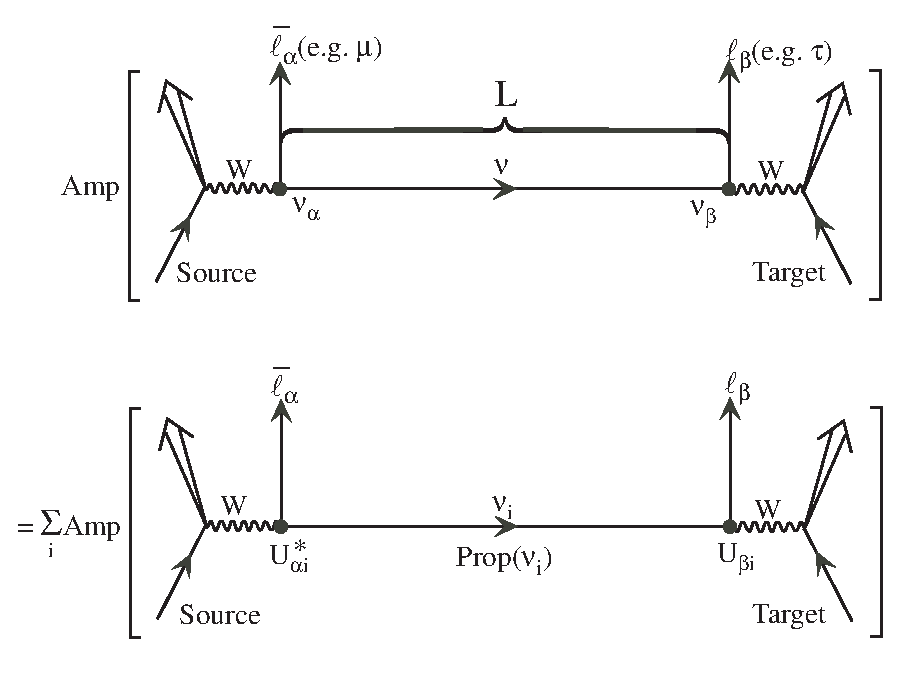
\includegraphics[width=0.98\textwidth]{images/Intro/SLAC_Fig1.eps}
  \caption[Neutrino flavour change (oscillation) in vacuum]{Neutrino
    flavour change (oscillation) in vacuum. “Amp” denotes an
    amplitude. Taken from~\cite{Kayser:2005cd}.}
  \label{fig:neutrinooscillationdiag}
\end{figure}

The oscillation relies on the hypothesis that the neutrino mass and
flavour states have the same momentum. These equations are developed
in the case of relativistic neutrino, which is true for all detectable
neutrinos\footnotemark.  It is worth noting that although this
derivation lacks physical motivation and robustness compared to a full
rigorous QFT approach, it leads to the exact same answer.

\footnotetext{The neutrinos have a mass smaller than few
  eVs~\cite{Troitsk}, and detectable neutrinos have energy greater
  than few hundreds of keVs~\cite{GALLEX1999}}

To show that neutrinos oscillate, one can start with the common
expressions of the flavours state as a function of the mass state via
the \Gls{PMNS} (Pontecorvo-Maki-Nakagawa-Sakata)
matrix~\cite{Pontecorvo:1967fh,Pontecorvo:1957cp,Bilenky:1978nj,Maki:1962mu}:

\begin{align}
  \colvec{
    \nu_e    \\
    \nu_\mu  \\
    \nu_\tau
  }
  &= \colvec{
    U_{e1} & U_{e2} & U_{e3}\\
  U_{\mu1} &U_{\mu2}  &U_{\mu3}\\
  U_{\tau1} &U_{\tau2}  &U_{\tau3}
                          }
  \colvec{
    \nu_1 \\
    \nu_2 \\
    \nu_3
  } \label{eq:pmnsugly}\\
  &=
  \colvec{
    1 & 0       & 0     \\
    0 & c_{23}  & s_{23} \\
    0 & -s_{23} & c_{23}
  }
  \colvec{
    c_{13}               & 0 & s_{13}e^{-i \delta_{\text{CP}}} \\
    0                    & 1 & 0                      \\
    -s_{13}e^{i \delta_{\text{CP}}} & 0 & c_{13}
  }
  \colvec{
    c_{12}  & s_{12} & 0 \\
    -s_{12} & c_{12} & 0 \\
    0      & 0      & 1
  }
  \colvec{
    1 & & \\
    & e^{-i\frac{\alpha_{21}}{2}} &\\
    & & e^{-i\frac{\alpha_{31}}{2}}\\
  }
  \colvec{
    \nu_1 \\
    \nu_2 \\
    \nu_3
  }                ,
  \label{eq:pmns}
\end{align}
which quantifies the massive content of the flavour neutrino $\nu_e$,
$\nu_\mu$ and $\nu_\tau$ according to their mass eigenstates $\nu_1$,
$\nu_2$ and $\nu_3$. Each $c_{ij}$ and $s_{ij}$ reads
$\cos\left(\theta_{ij}\right)$ and $\sin\left(\theta_{ij}\right)$
respectively, where $\theta_{ij}$ are the mixing
angles. $\delta_{\text{CP}}$ ($\alpha_{21}$, $\alpha_{31}$) are the
Dirac (Majorana) phases indicating \Gls{CP} (Charge Parity) violation.
Equation~\ref{eq:pmnsugly} is the general form for the \Gls{PMNS}
matrix, and Equation~\ref{eq:pmns} is a more elegant way to
parametrise it. Note that, in the absence of oscillations of the
active neutrinos to sterile neutrinos. Since there is no experimental
observations of oscillations to sterile neutrinos, these matrices
considered are unitary.

With Equation~\ref{eq:pmns}, one factorises in ``sectors'' the
oscillations according to the type of neutrino oscillation which are
observed. Hence, the first matrix relates to the ``atmospheric
sector,'' which, at first order, describes the oscillation of
$\nu_\mu\rightarrow\nu_\tau$. The third matrix describes the ``solar
sector'' that quantifies the oscillation of
$\nu_e\rightarrow\nu_\mu$. Finally, the second matrix is the ``cross
mixing'' matrix, which depends on the Dirac phase in its off-diagonal
terms. This phase encloses the difference in the oscillatory behaviour
between neutrinos and anti-neutrinos.

The calculation which leads to the conclusion that the neutrino of a
certain flavour oscillates to another during its propagation is now
quickly developed.

Supposing a neutrino of a defined flavour is created in space-time,
one can write:
\begin{equation}
  \label{eq:superposition}
  \ket{\nu_\alpha} = \sum_{k}U^{*}_{\alpha k} \ket{\nu_k} (\alpha = e,\mu,\tau),
\end{equation}
where \(\nu_\alpha\) are the flavour eigenstates and \(\nu_k\) are the
mass eigenstates. This is just another way of writing
Equation~\ref{eq:pmnsugly}. The term \(U^{*}_{\alpha k}\) is an
element of the mixing matrix. Next, the neutrino mass states are
orthogonal, so this leads to
\begin{equation}
  \braket{\nu_k|\nu_j}=\delta_{kj}
\end{equation}
and similarly for the flavour states:
\begin{equation}
  \braket{\nu_\alpha|\nu_\beta}=\delta_{\alpha\beta}.
\end{equation}

The massive states $\ket{\nu_k}$ are eigenstates of the Hamiltonian
operator $\mathcal{H}$:
\begin{equation}
  \mathcal{H}\ket{\nu_k}=E_k\ket{\nu_k},
\end{equation}
and, solving this equation, one reaches:
\begin{equation}
  \label{eq:schrodinger}
  \ket{\nu_k(t)} = \exp (-iE_k t)\ket{\nu_k}.
\end{equation}

Consider now a neutrino of flavour $\alpha$, that was created at
$t=0$, $\ket{\nu_\alpha(t=0)}$. This neutrino propagates in
space-time, using Equation~\ref{eq:schrodinger} and
\ref{eq:superposition}, one can write:
\begin{equation}
  \label{eq:prop} \ket{\nu_\alpha(t)} = \sum_k U_{\alpha
    k} \exp (-iE_kt)\ket{\nu_k},
\end{equation} for which, if $t=0$, $\ket{\nu_\alpha(t=0)} =
\ket{\nu_\alpha}$.

Note that it is possible to invert Equation~\ref{eq:superposition}:
\begin{equation}
  \label{eq:superpositioninvert} \ket{\nu_k}=\sum_\alpha U_{\alpha
k}\ket{\nu_\alpha},
\end{equation}
and that can be inserted into Equation~\ref{eq:prop}:
\begin{equation}
\ket{\nu_{\alpha}(t)}=\sum_{\beta=e,\mu,\tau}\left(\sum_{k}U^*_{\alpha
k}\exp\left(-iE_kt\right)U_{\beta k}\right)\ket{\nu_\beta}.
\end{equation}

Hence, for an arbitrary time $t$, one can see that the
$\ket{\nu_\alpha(t)}$ is a superposition of the states
$\ket{\nu_\beta}$. This means the neutrino created at $t=0$ is now a
composite state of the different flavour neutrinos. Consider now the
amplitude of the oscillation process
$\nu_\alpha\rightarrow \nu_\beta$,
$\mathcal{A}_{\nu_\alpha\rightarrow\nu_\beta}$:
\begin{align}
  \mathcal{A}_{\nu_\alpha\rightarrow\nu_\beta}(t) &= \braket{\nu_\beta|\nu_\alpha(t)}\\
                                                  &=\sum_kU^*_{\alpha k}U_{\beta k}\exp(-iE_kt),
\end{align}
which can be squared to get the probability of oscillation:
\begin{align}
  \mathcal{P}_{\nu_\alpha\rightarrow\nu_\beta} &= \left|\mathcal{A}_{\nu_\alpha\rightarrow\nu_\beta}\right|^2 \nonumber \\
                             &=\sum_{k,j}U^*_{\alpha k}U_{\beta k}U_{\alpha j}U^*_{\beta j}\exp\left(-i(E_k-E_j)t\right). \label{eq:prob}
\end{align}

Further simplification can be made to reach a simple equation. First,
the energy for any particle is given by:
\begin{equation}
  E_k=\sqrt{m_k^2+\vec{p}^{\,2}}
\end{equation}
and that can be simplified with a simple Taylor expansion for the case of
large momentum (i.e. relativistic particle):
\begin{equation}
  E_k\simeq |p|+\frac{m_k^2}{2|p|},
\end{equation}
which can be reinserted in the exponential term of Equation~(\ref{eq:prob}):
\begin{equation}
  E_k-E_j\simeq \frac{m_k^2-m_j^2}{2|p|}.
\end{equation}

In this equation, it is assumed that the momentum of the mass states
during the creation of the neutrino is the same, $p$. One can then
define $\Delta m_{kj}^2 = m_k^2-m_j^2$, and replace $|p|$ by $E$ since
the neutrinos are ultra-relativistic. Substituing everything in
Equation~(\ref{eq:prob}) leads to:
\begin{equation}
  \mathcal{P}_{\nu_\alpha\rightarrow\nu_\beta}=\sum_{k,j}U^*_{\alpha k}U_{\beta k}U_{\alpha j}U^*_{\beta j}\exp\left(-i(\Delta m_{kj}^2)t/(2E)\right).
\end{equation}

One further simplification comes from the fact that the neutrino are
propagating at almost the speed of light, $c$, which equates 1 in
natural units. So $t=L$, where $L$ is the distance of propagation of
the neutrino:

\begin{equation}
  \mathcal{P}_{\nu_\alpha\rightarrow\nu_\beta}=\sum_{k,j}U^*_{\alpha k}U_{\beta k}U_{\alpha j}U^*_{\beta j}\exp\left(-i(\Delta m_{kj}^2)L/(2E)\right).
\end{equation}

Finally, this probability can be simplified to:
\begin{align}
  \label{eq:oscilprob}
  \mathcal{P}_{\nu_\alpha\rightarrow\nu_\beta} =\delta_{\alpha\beta}&-4\sum_{k>j}\mathcal{Re}\left[U^*_{\alpha k}U_{\beta k}U_{\alpha j}U^*_{\beta j} \right]\sin^2\left(\frac{\Delta m^2_{kj}L}{4E}\right)  \nonumber \\
                                                                    &+2\sum_{k>j}\mathcal{Im}\left[U^*_{\alpha k}U_{\beta k}U_{\alpha j}U^*_{\beta j}\right]\sin\left(\frac{\Delta m_{kj}^2L}{2E}\right).
\end{align}

Note that the oscillation probability depends on terms of the form
$U^*_{\alpha k}U_{\beta k}U_{\alpha j}U^*_{\beta j}$ for which the
Majorana phases systematically cancel, which is why neutrino
oscillation experiments cannot detect these phases. These Majorana
phases can be determined via the detection of neutrinoless double beta
decay processes~\cite{Furry1939}.

In the case of \Gls{TK}, which measures electron neutrinos in a muon
neutrino beam of~600~MeV at a distance of 295~km, the oscillation
probability, Equation~\ref{eq:oscilprob},
becomes~\cite{Cervera:2000kp}:

\begin{align}
  \label{eq:numu-numu}
  \mathcal{P}_{\nu_\mu\rightarrow\nu_\mu} &= \mathcal{P}_{\bar{\nu}_\mu\rightarrow\bar{\nu}_\mu}\\
                                          &\simeq 1 - 4\cos^2\theta_{13}\sin^2\theta_{23}\left[1-\cos^2\theta_{13}\sin^2\theta_{23}\right]\sin^2\left(\frac{\Delta m^2_{32}L}{4E}\right), \nonumber
\end{align}
for the muon neutrino survival probability and
\begin{align}
  \mathcal{P}(\bbar{\nu}_{\mu} \rightarrow \bbar{\nu}_e) &\simeq \sin^2\theta_{23} \sin^22\theta_{13} \sin^2\left(\frac{\Delta m^2_{31} L}{4E}\right) \nonumber \\
                                                         &\bplus{-} \text{~}\frac{\sin2\theta_{12} \sin2\theta_{23}}{2\sin\theta_{13}} \sin\left(\frac{\Delta m^2_{21} L}{4E}\right) \times \sin^22\theta_{13} \sin^2\left(\frac{\Delta m^2_{31} L}{4E}\right) \sin\delta_{CP},
  \label{eq:numu-nue}
\end{align}
for the electron (anti-) neutrino appearance
probability. Figure~\ref{fig:oscillationprob} shows these oscillation
probabilities in the case of \Gls{TK} for typical values of the
parameters measured at \Gls{TK} (and reported in
Table~\ref{tab:oscillation_parameters}).

\begin{figure}[ht]
  \center
  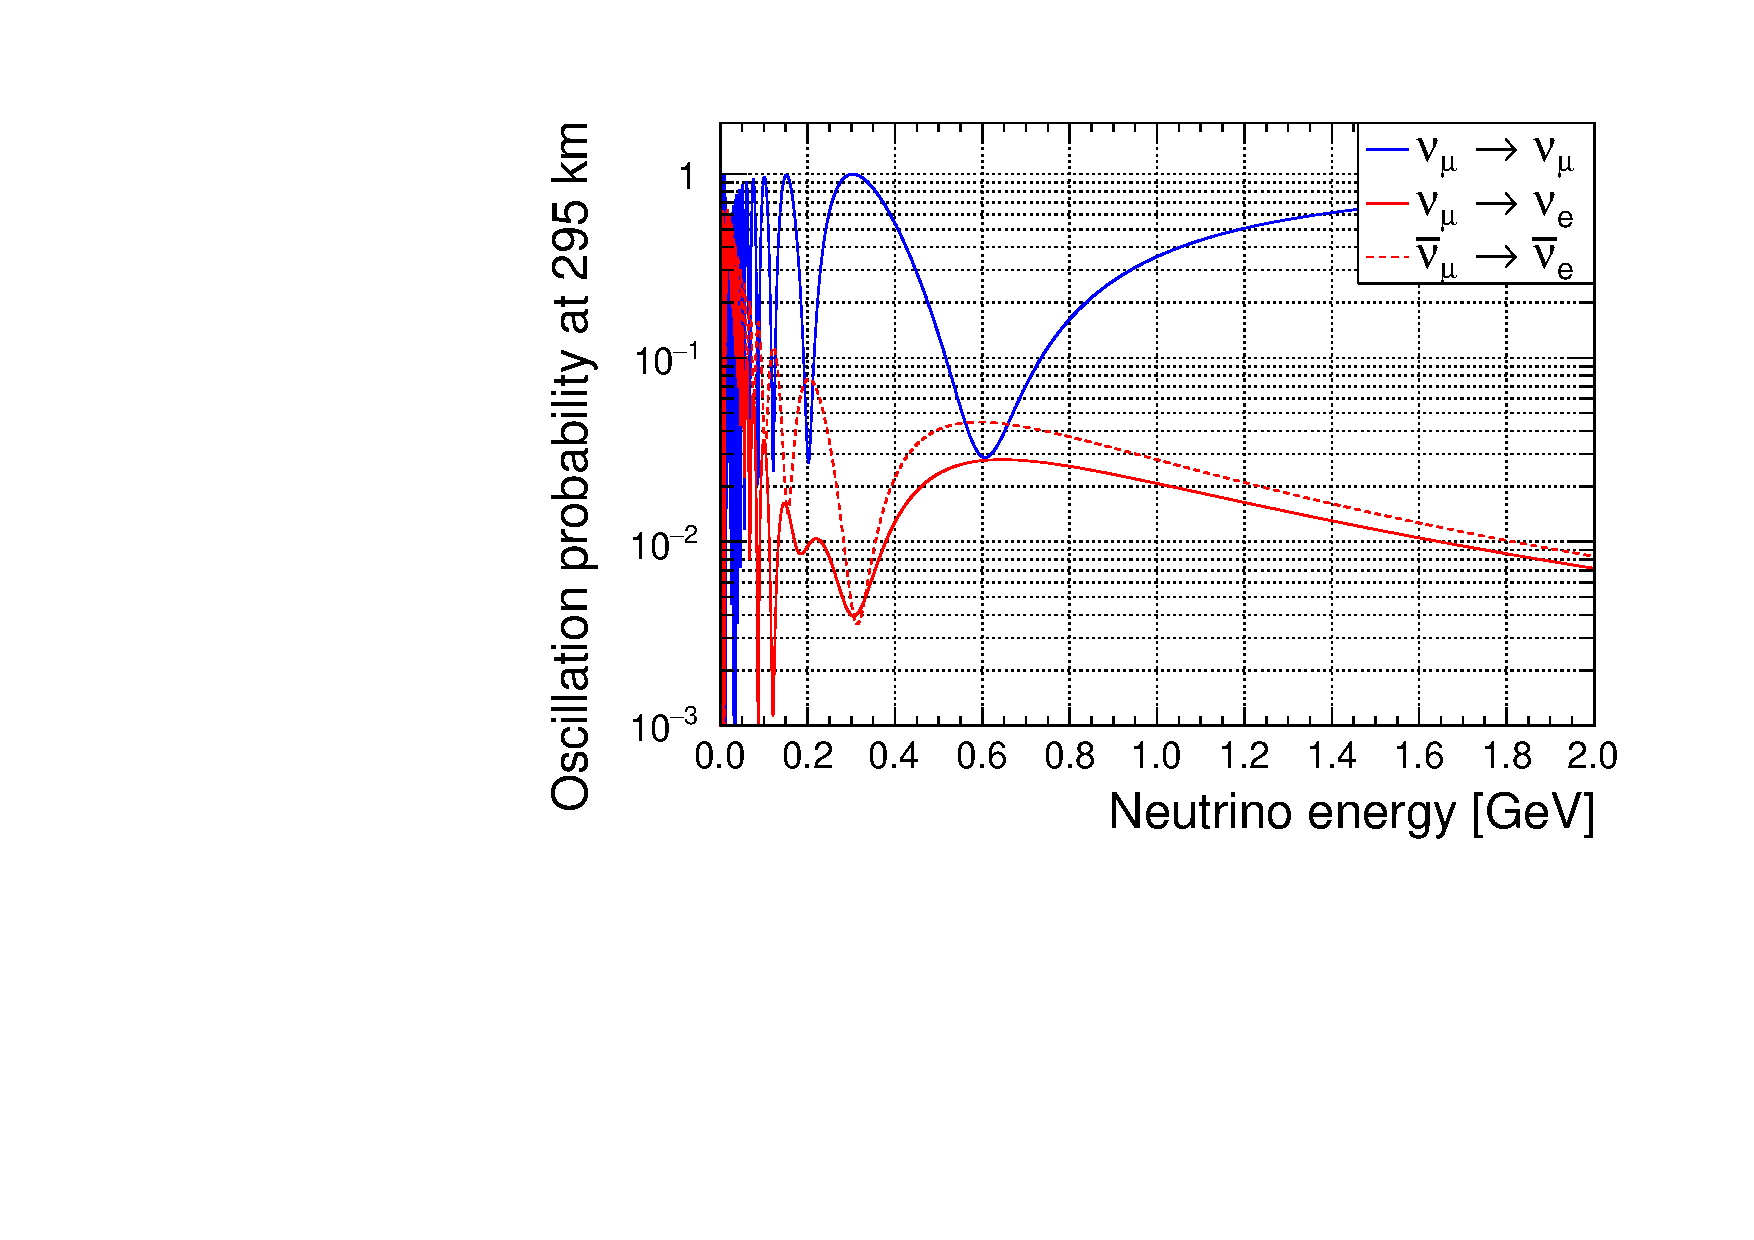
\includegraphics[width=0.8\textwidth]{images/Intro/Oscillation.pdf}
  \caption[Neutrino oscillation probability at T2K]{Neutrino
    oscillation probability at \Gls{TK}, for normal ordering,
    $\delta_{CP}=\pi/2$ and using the values given in
    Table~\ref{tab:oscillation_parameters}. Produced with
    Prob3++~\cite{prob3pp}.}
  \label{fig:oscillationprob}
\end{figure}


The Dirac phase, $\delta_{CP}$, is the last of parameter of the matrix
that remains to be measured. All the \Gls{PMNS} angles value are given
in Table~\ref{tab:oscillation_parameters}, along with the differences
of mass squared, $|\Delta m^2_{jk}|$. Note that this table
differentiates the normal and inverted ordering: this is because
neutrino oscillations are yet insensitive to the sign of the mass of
the atmospheric mass squared splitting. This can be seen in both
Equation~(\ref{eq:numu-numu}) and (\ref{eq:numu-nue}): the first,
dominant, term always appears squared
($\sin^2\left(\frac{\Delta m^2_{32}L}{4E}\right)$, for example), hence
experiments still do not have access to signs of $\Delta m_{31}$ and
$\Delta m_{32}$. Both hypotheses for the mass ordering are illustrated
in Figure~\ref{fig:ordering}. In the normal ordering case (left of the
figure), the mass states are ordered by increasing order:
$m_{\nu_1}<m_{\nu_2}<m_{\nu_3}$; in the inverted case (right of the
figure), the mass states are ordered in a different way:
$m_{\nu_3}<m_{\nu_1}<m_{\nu_2}$.

\begin{figure}[ht]
  \center
  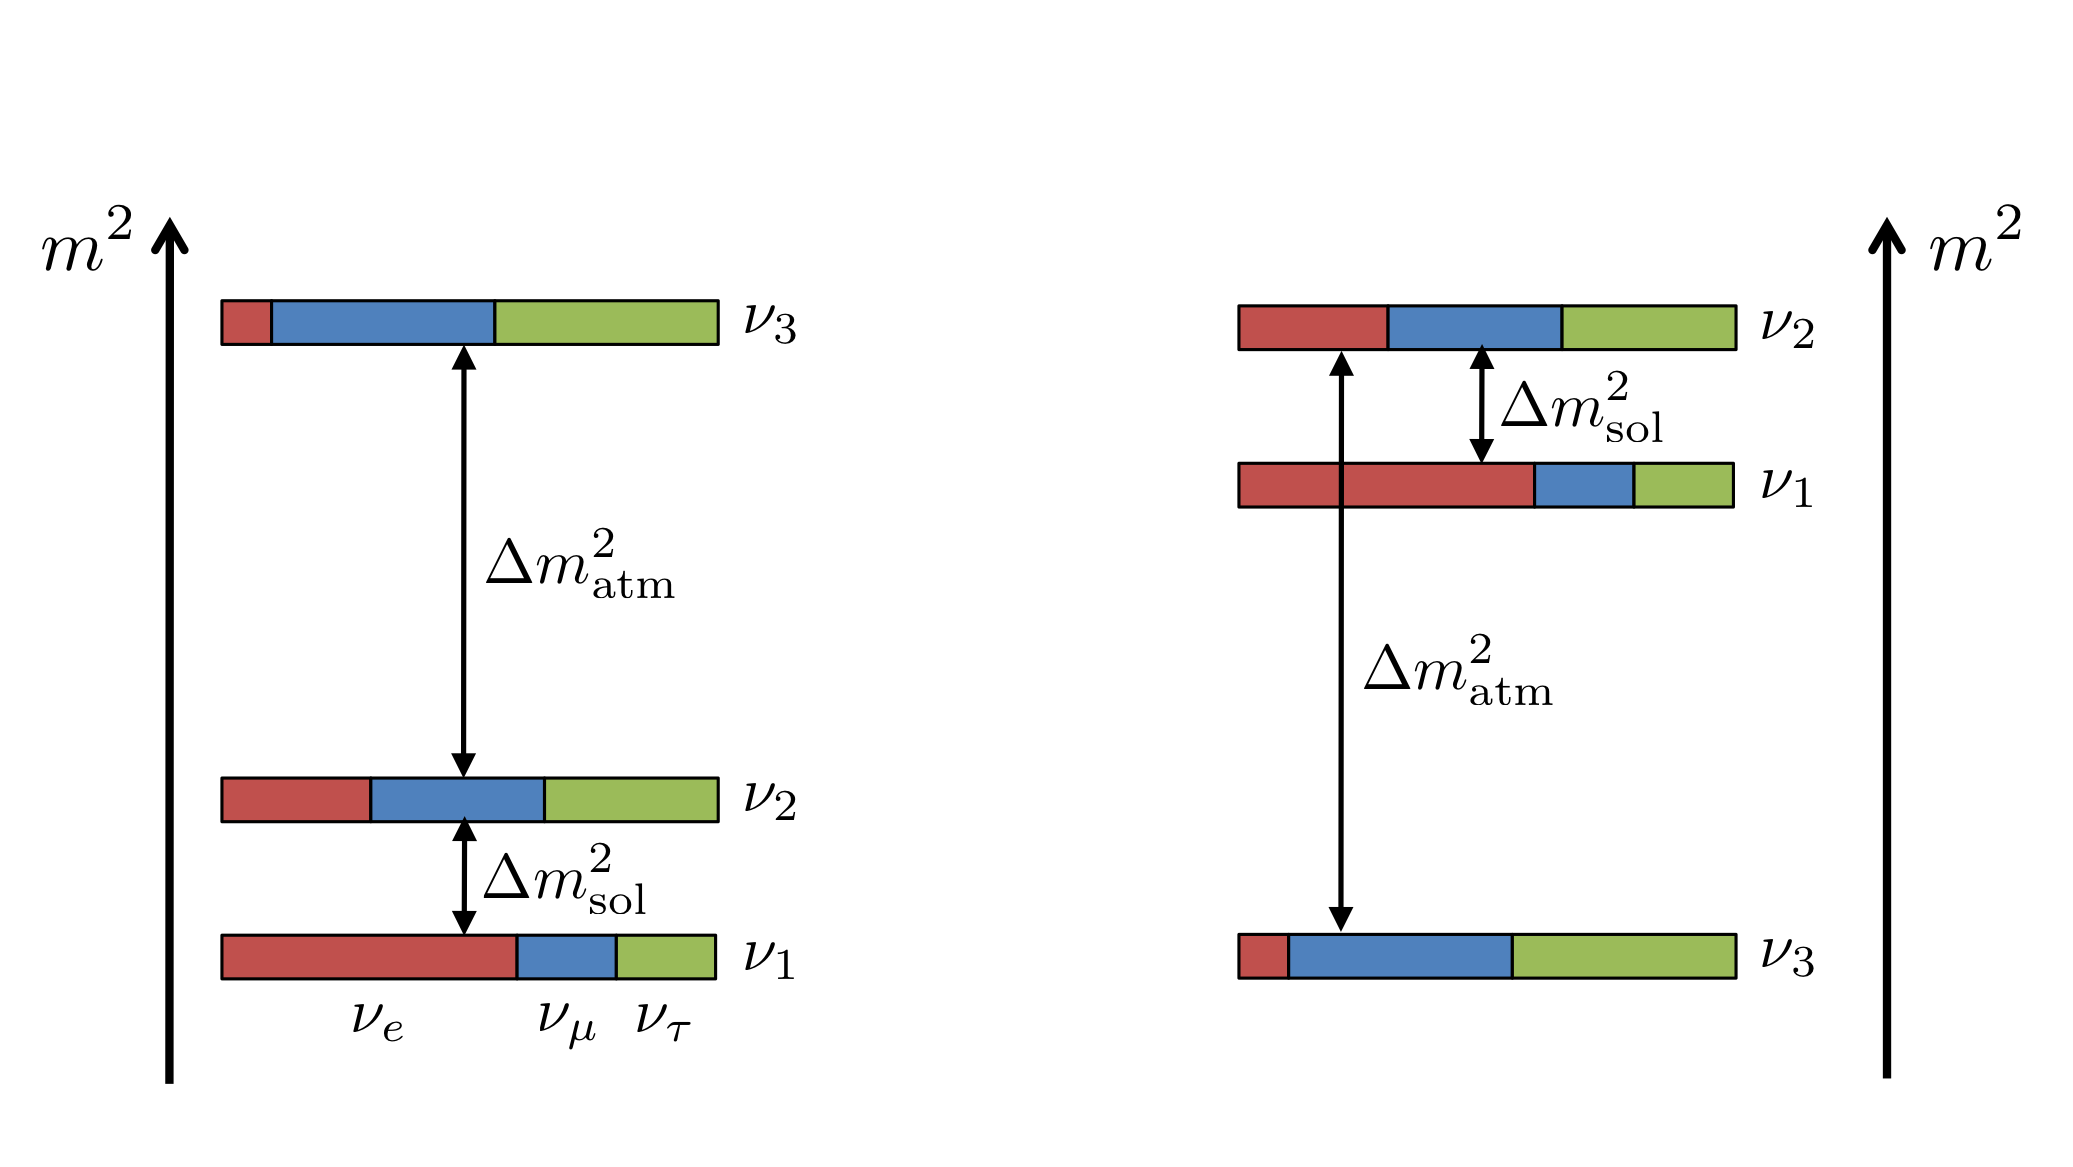
\includegraphics[width=0.8\textwidth]{images/Intro/mass-hierarchy.png}
  \caption[Possible neutrino mass ordering]{Possible neutrino mass
    ordering. \textbf{\textit{Left:}} Normal ordering
    case. \textbf{\textit{Right:}} Inverted ordering case. Reproduced
    from~\cite{massordering}}
  \label{fig:ordering}
\end{figure}





\begin{table}[ht!]
  \begin{adjustbox}{center}
    \begin{tabular}{llll}
      \toprule
      Parameter & Ordering & Best fit value& $3 \sigma$ range  \\
      \midrule%---------------------------------------------------------------------
      $\Delta m_{21}^2/10^{-5}~\mathrm{eV}^2 $ & NO, IO, Any & 7.37 & 6.93 -- 7.96 \\
      \midrule%---------------------------------------------------------------------
      $\sin^2 \theta_{12}/10^{-1}$        & NO, IO, Any & 2.97 & 2.50 -- 3.54 \\
      \midrule%---------------------------------------------------------------------
      $|\Delta m^2|/10^{-3}~\mathrm{eV}^2 $ & NO  & 2.525 & 2.411 -- 2.646 \\
                & IO  & 2.505 & 2.390 -- 2.624 \\
                & Any & 2.525 & 2.411 -- 2.646 \\
      \midrule%---------------------------------------------------------------------
      $\sin^2 \theta_{13}/10^{-2}$ & NO  & 2.15 & 1.90 -- 2.40 \\
                & IO  & 2.16 & 1.90 -- 2.42 \\
                & Any & 2.15 & 1.90 -- 2.40 \\
      \midrule%---------------------------------------------------------------------
      $\sin^2 \theta_{23}/10^{-1}$ & NO  & 4.25 & 3.81 -- 6.15 \\
                & IO  & 5.89 & 3.84 -- 6.36 \\
                & Any & 4.25 & 3.81 -- 6.26 \\
      \midrule%---------------------------------------------------------------------
      $\delta_{\text{CP}}/\pi$ & NO  & 1.38 & 0 -- 0.17 $\oplus$ 0.76 -- 2 \\
                & IO  & 1.31 & 0 -- 0.15 $\oplus$ 0.69 -- 2 \\
                & Any & 1.38 & 0 -- 0.17 $\oplus$ 0.76 -- 2 \\
      \bottomrule  
   \end{tabular}
   \end{adjustbox}
   \caption[Current neutrino oscillation parameters]{Neutrino
     oscillation parameters as described in the text, with their
     current best fit value and their $3\sigma$ range. This is shown
     for each mass ordering (``NO'': Normal Ordering ; ``IO'':
     Inverted Ordering), and for the absolute minimum with the mass
     ordering marginalised (``Any'' in the table).
     $\Delta m_{21}^2/10^{-5}~\mathrm{eV}^2 $ The first two parameters
     ($\Delta m_{21}^2/10^{-5}~\mathrm{eV}^2 $ and
     $\sin^2 \theta_{12}/10^{-1}$) are insensitive to mass
     ordering. $\Delta m^2$ is defined as $m_3^2 - (m^2_1+m^2_2)/2$,
     and $\Delta m_{21}^{2} = m^2_2-m^2_1$. Reproduced
     from~\cite{2017Capozzi}.}

\label{tab:oscillation_parameters}
\end{table}
\clearpage

%%% Local Variables:
%%% mode: latex
%%% TeX-master: Thesis
%%% End:


\section{Medium energy neutrino scattering physics}
\label{sec:crosssection}

This section describes the current state of the neutrino cross
sections for energies of order of $1$~GeV. Good knowledge of the
neutrino cross section is fundamental in neutrino accelerator
experiment, the introduction of this paragraph explains why. Then, a
summary of the knowledge is made for the nuclear model and the
following processes: charged-current quasi-elastic, resonant, coherent
pion production and deep inelastic scattering. Finally the known
differences between muon and electron (anti-) neutrino scattering are
explained.

\subsection{Introduction}
\label{subsec:xsecintro}
Neutrino cross section predictions are one of the major inputs for any
oscillation experiment; a way to see this is to analyse the equation
that leads to the number of events that are seen in a detector. In the
case of neutrinos, this is:
\begin{equation}
  \label{eq:nevents}
  N(l_\text{rec})=\Phi(E_\text{true})\times \left(1-P(E_\text{true})\right)\times
  \sigma(E_\text{true}, l_\text{true}, A) \times
  \epsilon(l_\text{true})_\text{det} \times R(l_\text{true},
  l_\text{rec})
\end{equation}
where:
\begin{itemize}[noitemsep,topsep=0pt]
\item $N(l_\text{rec})$ refers to the number of events reconstructed
  in a detector in a particular differential bin of a reconstructed
  quantity $l_\text{rec}$ (usually lepton momentum or angle),
\item $\Phi(E_{\text{true}})$ is the flux (which depends on the true energy
  of the neutrino, $E_{\text{true}}$),
\item $P(E_\text{true})$ is the oscillation probability (that also
  depends on the baseline and the oscillation parameters, as seen in
  the Section~\ref{sec:oscillation}),
\item $\sigma(E_\text{true}, l_\text{true}, A)$ is the cross section,
  where $A$ is the target nucleus,
\item $\epsilon(l_\text{true})_\text{det}$ is the detector efficiency,
\item and $R(l_\text{true}, l_\text{rec})$ is the migration matrix (or
  ``smearing matrix'') containing the detector effects to go from
  $l_\text{true}$ to $l_\text{rec}$.
\end{itemize}
Note that this is an approximated equation, since all these quantities
are generally convoluted, rather than simply multiplied.

In most accelerator neutrino oscillation experiments, two detectors
are used; one is next to the neutrino source and measures
$N(l_\text{rec})$ in the special case where the oscillation
probability is zero and the second detector, far from the neutrino
source, measures the same quantity with a non-trivial oscillation
probability.

From the near detector measurement, one can extract a data-driven
constraint on the flux and~/~or the cross section. There are different
ways of doing this:
\begin{itemize}[noitemsep,topsep=0pt]
\item via a direct fit to the flux and cross section as
  is done in \Gls{TK} (as will be seen in Chapter~\ref{chap:banff}),
\item or by directly correcting the true neutrino energy and thus
  modifying the flux ({\it \`a la}
  \Gls{NOvA}~\cite{PhysRevLett.118.231801}).
\end{itemize}

Whichever method is used, the neutrino flux is then extrapolated to
the far detector, which has access to the oscillation probability that
one wants to measure. In the case of \Gls{TK}, the flux and cross
section parameters become ``nuisance'' parameters and errors will be
constrained by the fit with data from the near detector. In the case
of \Gls{NOvA}, the flux has a reduced error based on what was observed
at the near detector.

Most of the time, the targets at the near and far detectors are chosen
to be the same or similar. Complications generally appear in the case
where acceptances are different between the near and the far
detectors. This leads to selecting events from different phase spaces
of the cross section in the two detectors, and it is generally not
trivial to extrapolate the cross section for the different phase
spaces. Similarly, the cross section depends on the neutrino energy,
therefore if the neutrino energy distribution changes due to the
baseline or the oscillations, the importance of the different
processes will change. To be able to make the extrapolation (near to
far) as described, one needs to precisely know the cross section and
create shape and normalisation systematic errors that encapsulate the
flux, acceptance and target differences between the near and the far
detector. The risk is to underestimate the cross section errors at the
far detector after over-constraining the cross section with the near
detector data. This is a constant source of challenges within the
\Gls{TK} experiment, which forces us to understand and use recent
cross section calculations.

In this context, precise knowledge of cross section is required to
reach acceptable fits of the near detector data. In the next sections,
the main processes for neutrino scattering are described in the
context of neutrinos energy from 500~MeV to a few GeV. Although not
explicitly described here, all the neutral current equivalent
reactions do exist, however, due to the complexity of detection
(absence of lepton) and lesser interest for oscillation analysis, data
is more sparse, and models are generally under constrained. The
analysis in this thesis is a good example of the challenges one faces
for measuring these cross sections.

\begin{figure}[ht]
  \center
  \vspace{1cm}

  \textbf{\textit{1)}}\hspace{1cm}\begin{fmffile}{feynmandiag/ccqe}
    \begin{fmfgraph*}(27,27)
      \fmfstraight
      % \fmftop{i2,o2}
      \fmfleft{i1,i2}
      \fmfright{o1,o2}
      % \fmfbottom{i1,o1}
      \fmf{fermion}{i2,v1,o2}
      \fmflabel{$\nu_l$}{i2}
      \fmflabel{$l^{-}$}{o2}
      \fmf{fermion}{i1,v2,o1}
      \fmflabel{$n$}{i1}
      % 
      \fmf{photon,label=$W$}{v1,v2}
      \fmflabel{$p$}{o1}
    \end{fmfgraph*}
  \end{fmffile} 
  \hspace{2cm}
  \textbf{\textit{2)}}\hspace{1cm}\begin{fmffile}{feynmandiag/mec}
    \begin{fmfgraph*}(27,27)
      \fmfstraight
      % \fmftop{i4,o4}
      \fmfleft{i1,i2,i3,i4,i5}
      \fmfright{o1,o2,o3,o4,o5}
      % \fmfbottom{i4,o4}      

      \fmf{fermion}{i5,v5,o5} % neutrion
      \fmf{photon,label=$W$}{v5,v4}
      \fmf{fermion,tension=2}{i2,v2} % interacting neutron
      \fmf{plain,tension=2}{v2,v4} % interacting neutron
      \fmf{fermion}{v4,o2} % interacting neutron
      \fmf{dashes,tension=0.,label=$\pi$}{v2,v1}
      \fmf{phantom}{v3,v4}
      \fmf{fermion,tension=2}{i1,v1} % spectator proton
      \fmf{plain,tension=2}{v1,v3} % spectator proton
      \fmf{fermion}{v3,o1} % spectator proton

      \fmflabel{$\nu_l$}{i5}
      \fmflabel{$n$}{i2}
      \fmflabel{$p$}{i1}

      \fmflabel{$l^{-}$}{o5}
      \fmflabel{$p$}{o2}
      \fmflabel{$p$}{o1}
      % \fmfstraight
    \end{fmfgraph*}
  \end{fmffile}
  \\
  \vspace{1cm}
  \textbf{\textit{3)}}\hspace{1cm}\begin{fmffile}{feynmandiag/respion}
    \begin{fmfgraph*}(27,27)
      \fmfstraight
      \fmftop{i2,o3}
      \fmfleft{i1,b2,b3,i2}
      \fmfright{o1,o2,o3}
      \fmfbottom{i1,o1}
      \fmf{fermion,tension=1.5}{i2,v1}
      \fmflabel{$\nu_l$}{i2}
      \fmf{fermion}{v1,o3}
      \fmflabel{$l^{-}$}{o3}
      \fmf{fermion,tension=1.7}{i1,v2}
      \fmflabel{$p$}{i1}
      % \fmfstraight
      \fmf{dbl_plain_arrow,label=$\Delta^{++}$,tension=2}{v2,v3}
      \fmf{photon,label=$W$}{v1,v2}
      \fmf{dashes,tension=1.5}{v3,o2}
      \fmflabel{$\pi^{+}$}{o2}
      \fmf{fermion}{v3,o1}
      \fmflabel{$p$}{o1}
    \end{fmfgraph*}
  \end{fmffile}
  \hspace{2cm} 
  \textbf{\textit{4)}}\hspace{1cm}\begin{fmffile}{feynmandiag/dis}
    \begin{fmfgraph*}(27,27)
      \fmfstraight
      % \fmftop{i4,o4}
      \fmfleft{i1,i2,i3,bi1,bi2,i4}
      \fmfright{o1,o2,bo1,o3,bo2,o4}
      % \fmfbottom{i1,o1}
      \fmf{fermion}{i4,v1,o4}
      \fmflabel{$\nu_l$}{i4}
      \fmflabel{$l^{-}$}{o4}
      \fmf{fermion}{i3,v2,o3}
      \fmf{photon,label=$W$,tension=0.5}{v1,v2}
      \fmf{fermion}{i2,o2}
      \fmf{fermion}{i1,o1}
      \fmflabel{$u$}{i1}
      \fmflabel{$u$}{i2}
      \fmflabel{$d$}{i3}
      \fmflabel{$u$}{o1}
      \fmflabel{$u$}{o2}
      \fmflabel{$u$}{o3}
    \end{fmfgraph*}
  \end{fmffile}
  \\
  \vspace{1cm}
  \textbf{\textit{5)}}\hspace{1cm}\begin{fmffile}{feynmandiag/coh}
    \begin{fmfgraph*}(27,27)
      \fmfstraight
      \fmftop{i2,o4}
      \fmfleft{i1,b2,b3,i2}
      \fmfright{o1,o2,o3,o4}
      \fmf{fermion}{i2,v1}
      \fmflabel{$\nu_l$}{i2}
      \fmf{fermion}{v1,o4}
      \fmflabel{$l^{-}$}{o4}
      \fmf{fermion,tension=1.5}{i1,v2}
      \fmflabel{$A$}{i1}
      % \fmfstraight
      \fmf{photon,label=$W$}{v1,v2}
      % \fmflabel{$Z^0$}{v1}
      \fmf{photon}{v2,o2}
      \fmflabel{$\pi^{+}$}{o2}
      \fmf{fermion}{v2,o1}
      \fmflabel{$A$}{o1}
    \end{fmfgraph*}
  \end{fmffile}
  \caption[Main Feynman diagrams contributing to the total cross
  section of neutrinos from 500~MeV to a few GeV]{Main Feynman
    diagrams contributing to the total cross section of neutrinos from
    500~MeV to a few GeV: \textbf{\textit{1)}} charged-current
    quasi-elastic (\Gls{CCQE}) \textbf{\textit{2)}} charged-current
    multi-nucleons (charged-current 2 particles-2 holes, \gls{2p2h});
    \textbf{\textit{3)}} charged-current resonant pion production;
    \textbf{\textit{4)}} charged-current deep inelastic scattering
    (\Gls{DIS}); \textbf{\textit{5)}} charged-current coherent pion
    production.}
  \label{fig:xsecs_diag}
\end{figure}

\begin{figure}[ht]
  \center
  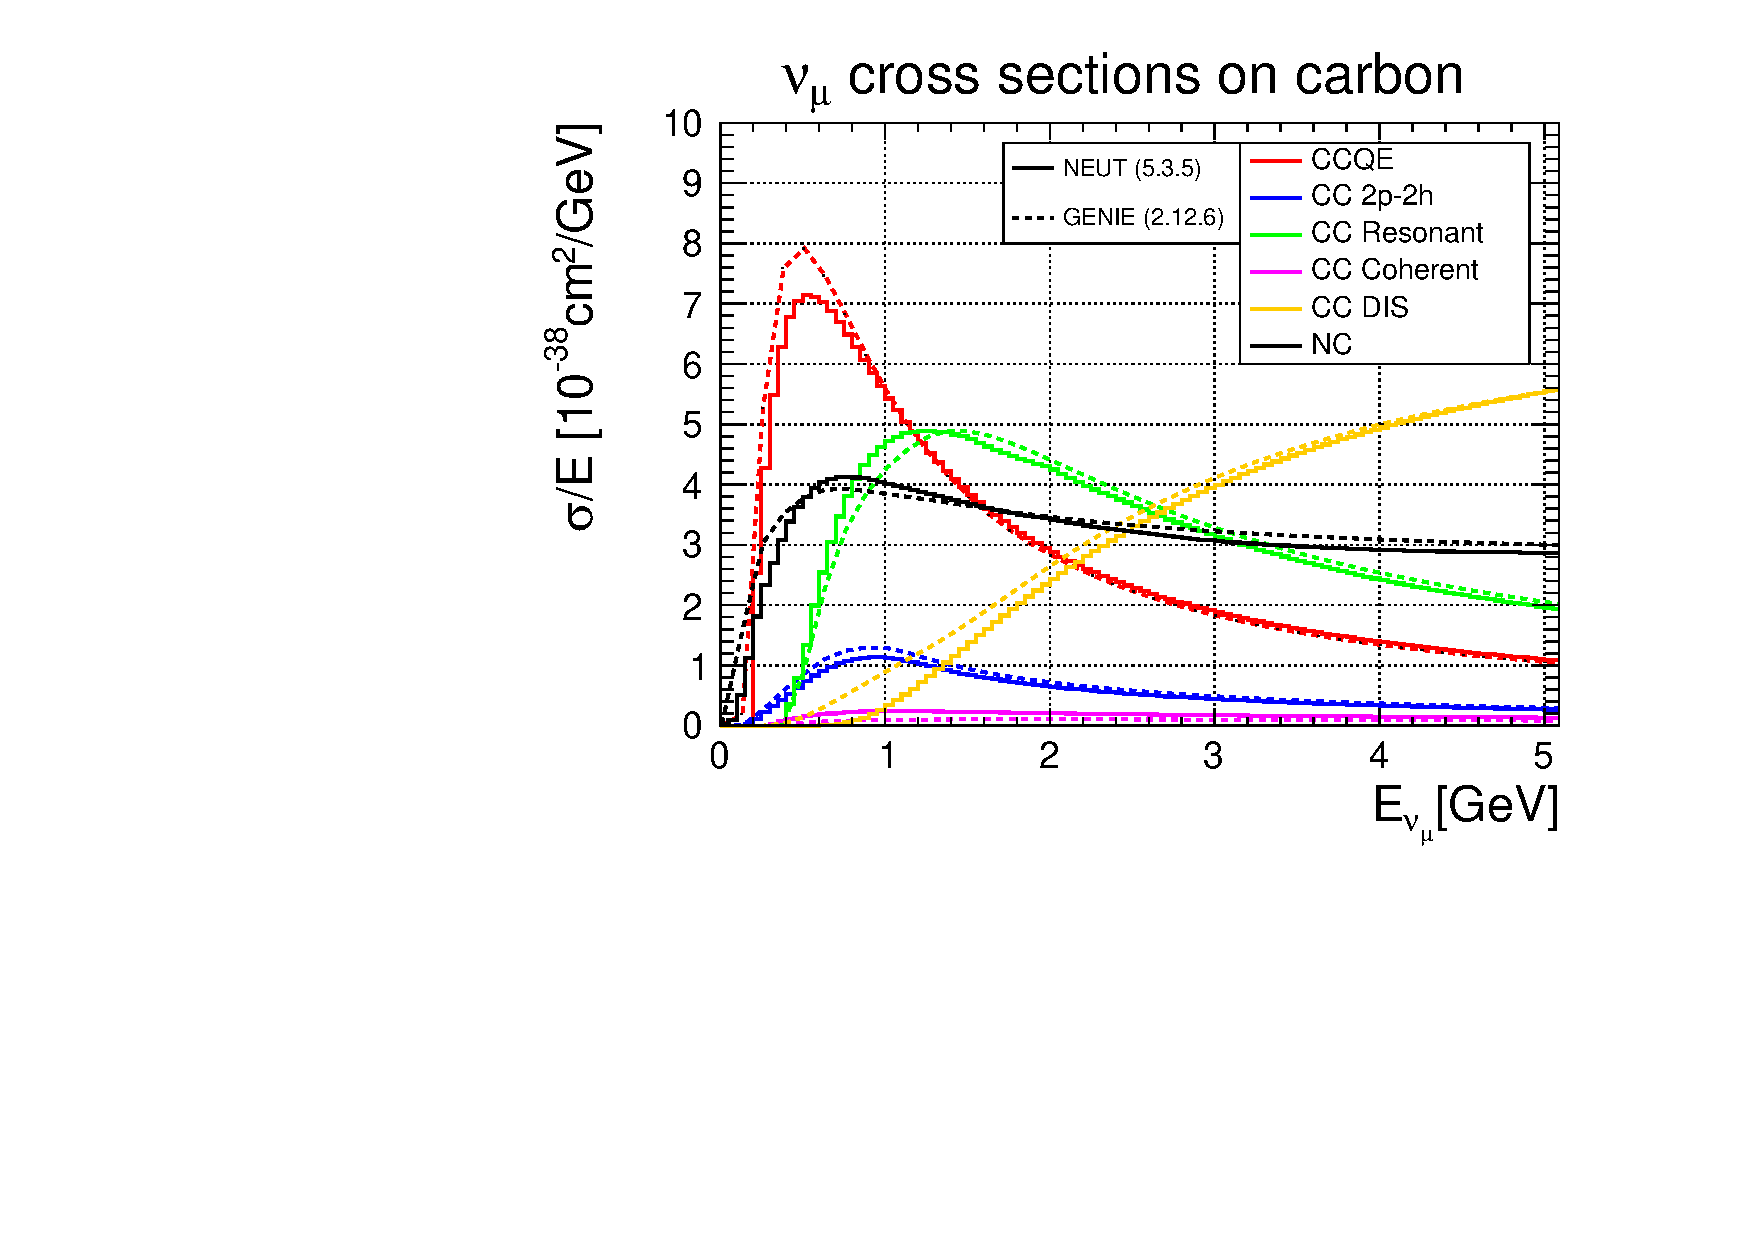
\includegraphics[width=0.7\textwidth]{images/Intro/cross_sections.pdf}
  \caption[Muon neutrino cross sections on carbon from GENIE and
  NEUT]{Muon neutrino cross sections on carbon from
    \Gls{GENIE}~\cite{GENIE1,GENIE2} and \Gls{NEUT}~\cite{NEUT}.}
  \label{fig:xsecs_plot}
\end{figure}

\subsection{Nuclear Model}
The nuclear model is purely related to the description of the nucleus,
it can be accessed via experiments such as electron scattering. One of
the most fundamental input to the nuclear model is the distribution of
momentum of the nucleons in the nucleus. There are several ways to
simulate this. The simplest of which is the Global Relativistic Fermi
Gas (\Gls{RFG}). In this model, the nucleons momentum simply follow a
Fermi distribution (the momentum of the nucleons is a quadratic
distribution up to the Fermi momentum, $p_F$), where the nuclear
matter is assumed to have a constant density, this is the default
model in \Gls{NEUT}, which is the neutrino interaction generator used
at \Gls{TK}.

The other model that was included in the \Gls{TK} simulations is the
Spectral Function (\Gls{SF}) model~\cite{Benhar}. In this model, all
the nucleon-nucleon interactions are factorised-out to produce a more
realistic distribution of the nucleon momentum in the nucleus. Note
that this model was significantly improved since its implementation in
the \Gls{NEUT} generator~\cite{Rocco:2016vyz}.

The \Gls{NEUT} \Gls{SF} models has proven to be insufficient to
predict \Gls{MINERVA} and \Gls{MiniBooNE} data~\cite{CallumFit}, so
the \Gls{RFG} model is used.

\subsection{Charged-Current Quasi-Elastic process}
\label{subsec:ccqe}
A Charged-Current Quasi-Elastic (\Gls{CCQE}) interaction is depicted
on the top left of Figure~\ref{fig:xsecs_diag}. In this process, a
(anti-) neutrino of a given flavour interacts with a single neutron
(proton) to create a negatively (positively) charged lepton of the
same flavour. These interactions can happen on free nucleon (hydrogen)
or nuclear target (carbon, oxygen), if the neutrino has enough energy
to create a charged lepton. The neutrino interacts via $W$-boson
exchange.

Since this is a two body process, momentum and energy conservation
laws can be used to reconstruct the energy of the neutrino. In the
case of a free nucleon, the reconstructed neutrino energy,
$E_\text{rec}$, is~\cite{MartiniERec}:
\begin{equation}
\label{eq:ereco}
E_{\text{rec}}=\frac{E_\text{l}-m_\text{l}^2/(2M)}
{1-\left(E_\text{l}-P_\text{l}\cos\left(\theta_\text{l}\right) \right)/M}
\end{equation}
where $E_\text{l}$ is the energy of the lepton (muon or electron),
$m_\text{l}$ is the lepton mass, $P_\text{l}$ its momentum,
$\cos\left(\theta_\text{l}\right)$ is the cosine of the lepton
scattering angle, and M is the mass of the struck nucleon (neutron for
neutrino and proton for anti-neutrino).

As can be seen in Figure~\ref{fig:xsecs_plot}, which shows the
neutrino cross section against its energy, the \Gls{CCQE} cross
section is largely dominant around 600~MeV, which is also the \Gls{TK}
peak energy. As will be described later, this is not a coincidence.

The formalism to calculate the value of the cross
section~\cite{LlewellynSmith} in the context of bubble chamber
experiments~\cite{ANLCCQE,BNLCCQE,CERNCCQE}. Most of the parameters
involved in the calculation of the cross section can be accessed via
electron scattering, however the cross section also depends on a
fundamental parameter which can only by accessed via neutrino
measurements, called the axial mass ($M_A^{QE}$).

The \Gls{CCQE} cross section is proportional to the following form
factor (so-called dipole form factor):
\begin{equation}
  \label{eq:ccqeff}
  F_A(Q^2) = \frac{g_A}{\left(1+\frac{Q^2}{M_A^{\text{QE~}2}}\right)^2}
\end{equation}
This form factor and $M_A^{QE}$ parameter are related to the spacial
extension of the nucleon for neutrino interactions by a inverse
Fourier transform. This has recently come into more focus as a dipole
form facbintor may not be justified for the neutrino
case~\cite{PhysRevD.93.113015,PhysRevD.92.113011}.

The description of the cross section quickly becomes more complicated
in the case of nuclear targets or even for
deuteron~\cite{SinghDeuteron}. In this case, corrections of various
kinds have to be applied~\cite{SmithMoniz,NievesCCinc}. Some of these
corrections are listed here:

\begin{itemize}
\item The nucleons have a binding energy in the nucleus, the
  consequence is that the excited nucleon after neutrino interaction
  has to have a over the Fermi energy to happen. If the excited
  nucleon does not go over this threshold, the event said to be Pauli
  blocked.
\item As was seen in the previous section, the nucleons move in the
  nucleus, the descriptions of the distribution of the nucleon
  momentum range from simple Global Relativistic Fermi Gas (\Gls{RFG})
  to more complex Spectral Functions~\cite{Benhar} or Local Fermi Gas
  (\Gls{LFG}).

  It is clear that depending on the nuclear model used, one will get
  different energy distributions for the initial state of the system
  just before the neutrino interaction. These models will produce
  different kinematics for the outgoing particle and ``Pauli block''
  different events.
\item The long range correlations has effect on $Q^2$ (which is the
  absolute value of the 4-momentum transfer squared): at low $Q^2$ the
  cross section is expected to be reduced; whereas it is enhanced at
  intermediate $Q^2$ and goes back to unity for
  $Q^2\rightarrow \infty $.  This correction, also refered as ``Random
  Phase Approximation'' (\Gls{RPA})~\cite{NievesCCinc} is due to the
  fact that the $W$-boson creates virtual particle-holes in the
  nuclear medium in which it is propagating.
\end{itemize}

It should be noted that most of our knowledge in the \Gls{CCQE} cross
section stems from bubble chamber
data~\cite{ANLCCQE,BNLCCQE,CERNCCQE}. Nuclear targets experiments such
as \Gls{MINERVA}~\cite{MinervaNuCCQE},
\Gls{MiniBooNE}~\cite{MiniBooNENuCCQE} and, in a lesser extent,
\Gls{TK}~\cite{T2KCCQE} and \Gls{K2K}~\cite{K2KCCQE} near detectors
data are still challenging to interpret. One of the reasons being that
these measurements cannot disentangle the multi-nucleon processes from
the pure \Gls{CCQE} contributions~\cite{CallumFit}. Indeed, all the
\Gls{CC}$0\pi$\footnote{\Gls{CC} with no pion in the final state
  measurements, as opposed to direct measurements of the \Gls{CCQE}
  measurements, includes events where pions are created in the nucleus
  but do not exit the nucleus, or events where several nucleons escape
  the nucleus.} measurements on nuclear targets show that the data is
higher than the one would get by only considering the \Gls{CCQE} cross
section. This hints towards the presence of another contribution.

\subsection{Multi-nucleon processes}
Multi-nucleon processes, also called ``np-nh'' for n-particles n-holes
(or even sometimes loosely referred as Meson Exchange Current
(\Gls{MEC})) are those processes where the neutrino interacts with a
correlated pair of nucleons. The cross section for these events to
happen is smaller than one for \Gls{CCQE} processes as can be seen in
Figure~\ref{fig:xsecs_plot}. They also are largely more complex to
calculate and to measure. This makes them one of the primary focuses
in the neutrino cross section community.

Due to their similarity with pure \Gls{CCQE} events, these events lead
to an enhancement to the total number of expected \Gls{CC}$0\pi$
events as explained earlier. An example of one of the many
contributing Feynman diagrams for this cross section is shown in top
right of Figure~\ref{fig:xsecs_diag}, where the similarity with
\Gls{CCQE} processes is clearer. Three main calculations for the
multi-nucleon cross section were done recently
in~\cite{MartiniNpNh1,MartiniNpNh2}, \cite{NievesNpNh1,NievesNpNh2}
and \cite{AmaroNpNh1,AmaroNpNh2}.

Note that despite the similarity in topology with the pure \Gls{CCQE}
processes, the reconstructed energy in
Equation~\ref{eq:ereco}~\cite{MartiniERec} does not hold for these
events since this is no longer a two body process.

np-nh events are by definition nuclear processes which can only be
accessed by modern neutrino experiments using a nuclear target, and
the corrections listed in the previous section need to be applied to
reliably calculate its cross section. Most of the knowledge on these
processes originates from experiments such as \Gls{K2K}~\cite{K2KCCQE}
and \Gls{MiniBooNE}~\cite{MiniBooNENuCCQE,MiniBooNEANuCCQE}, which
were the first to see the effect of these processes (enhancement of
the \Gls{CC}$0\pi$ cross section); these were followed a few years
later by \Gls{TK}~\cite{T2KCCQE}. More recently, the \Gls{MINERVA}
experiment released data which proves that our understanding of this
cross section is still very limited~\cite{minervaq3q0}. This
measurement shows that one needs to multiply the np-nh cross section
by a factor of two to fit the data. This is still a puzzle, which no
nuclear theorist has been able to explain yet.

The way to shed light on these processes will probably come from the
observation of the protons exiting the nucleus, with use of the
precise detectors in the Fermilab Short Baseline Neutrino
program~\cite{SBN,microboone}, although the theoretical calculations
of proton kinematics are still at their early
stage~\cite{MartiniProtonKine} (for example they are only available
for carbon and do not include interactions of the exiting protons with
the nuclear medium).



\subsection{Resonant processes}
\label{subsec:res}
\begin{figure}[ht]
  \center
  \hspace{1cm}\begin{fmffile}{feynmandiag/qsqw}
    \begin{fmfgraph*}(27,27)
      \fmfstraight
      \fmftop{i2,o3}
      \fmfleft{i1,b2,b3,i2}
      \fmfright{o1,o2,bo1,bo2,o3}
      \fmfbottom{i1,o1}
      \fmf{fermion,tension=1.5}{i2,v1}
      \fmflabel{$\nu$}{i2}
      \fmf{fermion}{v1,o3}
      \fmflabel{$l$}{o3}
      \fmf{fermion}{i1,v2}
      \fmflabel{$n/p$}{i1}
      \fmf{photon,label=$Z^0/W$}{v1,v2}
      \fmf{fermion,tension=0.5}{v2,o2}
      \fmflabel{$X, W_{inv}$}{o2}
      \fmf{fermion,tension=0.5}{v2,o1}
      \fmffreeze
      \fmfcmd{style_def marrowQ expr p = drawarrow subpath (1/4, 3/4) of p shifted 6 right
        withpen pencircle scaled 0.4; label.top(btex $Q^2$ etex, point 0.5 of p
        shifted 15 right shifted 6 down); enddef;}
      \fmf{marrowQ}{v1,v2}
    \end{fmfgraph*}
  \end{fmffile}
  \vspace{0.3cm}
  \caption[Illustration of the $Q^2$ and $W_{inv}$ quantities for a
  generic neutrino reaction]{Illustration of the $Q^2$ and $W_{inv}$
    quantities for a generic neutrino reaction. $l$ denotes a charged
    lepton or a neutrino of the same flavour as the incoming one
    ($\nu$), depending on whether the interaction is Charged-Current
    ($W$) or Neutral-Current ($Z^0$). The $X$ denotes any particle(s)
    of total energy $W_{inv}$ that has been generated by the boson
    interaction on a nucleon. In the case of a resonant interaction,
    the $X$ would be a nuclear resonance that decays into a pion or a
    photon, and a nucleon.}
  \label{fig:FeynmanQ2W}
\end{figure}

A Charged-Current Resonant (\Gls{CC}\Gls{RES}) process is illustrated
in the middle left of the Figure~\ref{fig:xsecs_diag}. In the case of
a resonant interaction, rather than interacting ``elastically'' with a
nucleon, the $W$-boson has enough energy to create a ``nuclear
resonance,'' which, in simple terms, can be seen as equivalent to
flipping the spin of a valence quark in the proton, and changing the
isospin of one or several of the quarks. The resonance usually
undergoes a strong decay by emitting of a pion and a nucleon. The
resonance created is a much more complex object than a simple Dirac
spinor and the calculation of the amplitudes of this cross section is
more involved mathematically than in the case of
\Gls{CCQE}~\cite{Rein1,Rein2}.

These \Gls{RES} cross sections are usually parametrised by a
double differential cross section of the form
$\frac{d^2\sigma}{dQ^2dW_{inv}}$, where $Q^2$ is the absolute value of
the 4-momentum transfer squared and $W_{inv}$ is the invariant mass of
the outgoing hadron system. These quantities are illustrated in
Figure~\ref{fig:FeynmanQ2W}.

Some additional corrections due to the nuclear environment have to be
taken into account for reliable cross section predictions. The main of
which are the Final State Interactions (\Gls{FSI}). These affect the
exiting pions and can change the topology of the events if a pion is
absorbed, for example. Another correction can be applied on the
resonance, since it can also scatter with a nucleon during its very
short life-time. This leads to processes such as pion-less delta
decays or a change in the decay width of the
resonance~\cite{Oset1987,Singh1998}.

Also, note that there exist several resonances ($\Delta_{1232}$ having
the lowest mass of them, and contributing the most to the amplitude)
and a non-resonant ``background''~\cite{Background} (where the nucleon
is used as a propagator between the interacting boson and the decay to
pion and nucleon). These different contributions produce the same
final states and the amplitudes for each of them needs to be added
coherently to correctly take into account interferences. These
interferences can significantly modify the topology of the single pion
events~\cite{Minoo}.

As it was the case for \Gls{CCQE}, most of the models are constrained
by the bubble chamber experiments~\cite{ANLPion,ANLNCPion,BNLPion},
although there is still some confusion in the compatibility between
these data sets~\cite{Wilkinson:2014yfa}. The
\Gls{MINERVA}~\cite{MINERvACCPion},
\Gls{MiniBooNE}~\cite{MiniBooNECC1PiP,MiniBooNECC1Piz,MiniBooNENCPi0},
\Gls{K2K}~\cite{K2KPion} and \Gls{TK} data are still a long way from
being understood within an unique framework.

\subsection{Deep Inelastic Scattering processes}
The Deep Inelastic Scattering (\Gls{DIS}) processes occur at higher
energies when the $W$-boson interacts with a single quark. The process
is illustrated in Figure~\ref{fig:xsecs_diag} (bottom right). In DIS
events, many pions are usually created.

This process can be calculated from first principles but relies on the
precise knowledge of the parton distribution functions, at low $Q^2$
and relatively high $x$\footnote{$Q^2$ is the momentum transfer of the
  probe to the target, and $x$ is defined as $\frac{Q^2}{2M\omega}$,
  where M is the target mass (if at rest) and $\omega$ is the energy
  transfer.\label{ftn:qsquare}} regions, for which scaling violations
occurs and DGLAP equations, which are used to extrapolate \Gls{PDF}
across $Q^2$, do not hold~\cite{DGLAP1,DGLAP2,DGLAP3,DGLAP4}.

Most of the data used for the \Gls{PDF} (Parton Distribution
Functions) fits come from \Gls{NuTEV}~\cite{nutev},
\Gls{CHORUS}~\cite{chorus} and \Gls{CDHSW}~\cite{CDHSW}. From these,
it is still unclear whether coupled \Gls{DIS}~/~nuclear effects such
as the \Gls{EMC} effect or the \gls{anti-shadowing} happen for
neutrino interactions. These phenomena are observed in \Gls{DIS}
electron scattering: it was shown that the nuclear cross section is
enhanced in certain regions of $x$ compared to the one of the free
nucleon. They have unclear theoretical explanations.

Some more recent data from \Gls{MINERVA}~\cite{Mousseau} is hinting
towards the same conclusion (absence of anti-shadowing effect).

For the hadronisation physics, it was recently noted that the
\Gls{HERMES} data~\cite{HERMES} could used to better predict some
basic quantities related to hadron
multiplicities~\cite{Katori:2014fxa}.

These processes need to be carefully studied in the context of higher
energy beams, such as the \Gls{DUNE}~\cite{DUNE1,DUNE2,DUNE3,DUNE4}
one, or \Gls{NOvA}~\cite{Ayres:2007tu} and atmospheric neutrino
experiments~\cite{Aartsen:2014oha}.

\subsection{Shallow Inelastic Scattering processes}
Between the \Gls{RES} and \Gls{DIS}, other processes called Shallow
Ineslastic Scattering processes can happen. This is refered
theoretically as the ``transition region.'' These processes are added
because the regions of validity of the \Gls{RES} and \Gls{DIS} cross
sections are disjoint. In practice, the problem is overcome by using
the continuum (background term) of the \Gls{RES} cross section and
ensuring continuity in the $W$ variable~\cite{GENIE1}.

Although these channels are very important in the context of
\Gls{NOvA} (because the neutrino energy distribution peaks at 2~GeV),
there are still little theoretical calculations. A last notable
reference is a two pions neutrino production calculation
in~\cite{Hernandez:2007ej}.

\subsection{Coherent pion production processes}
The coherent processes happen when the $W$-boson from the neutrino has
a very low momentum and cannot resolve individual nucleons inside the
nucleus~\cite{Rein:2006di,Berger:2008xs}. In that case, the boson
interacts with the whole nucleus. A pion is created from de-excitation
of the nucleus and critically, this pion does not undergo final state
interactions. Only recent nuclear data is sensitive to the coherent
pion production processes, historical measurements date from 1988 with
the experiments SKAT, BEBC, CHARM-II and
E632~\cite{Grabosch:1985mt,Allport:1988cq,Vilain:1993sf,Aderholz:1988cs},
that measured neutrino coherent pion production on neon. More modern
experiments also tried to measure the coherent interaction on plastic
scintillator, at the beginning unsuccessfully
(\Gls{K2K}~\cite{Hasegawa:2005td} and
\Gls{SciBooNE}~\cite{PhysRevD.78.112004}). The first charged-current
measurement on plastic scintillator was made by
\Gls{MINERVA}~\cite{Higuera:2014azj}, and was followed by
\Gls{TK}~\cite{Abe:2016fic}. \Gls{ArgoNeuT}~\cite{Acciarri:2014eit}
also measured these interactions on liquid argon.

\subsection{Electron neutrino cross sections}
\label{subsec:electronnu}
Electron neutrino cross sections have the same contributing Feynman
diagrams as the ones shown in Figure~\ref{fig:xsecs_diag}. There are
further differences expected since the fact that electrons have a
smaller mass than muons opens phase space when one compares muon
neutrino to electron neutrino cross sections. Further complications
arise for the so-called Second Class Current (\Gls{SCC}) and radiative
corrections~\cite{Day:2012gb}. The electron neutrino cross section in
these energies always suffers from having very low statistical power
(few events), since it is simpler to create an muon neutrino beam as
will be seen later (Section~\ref{sec:t2kbeamline}). The current
knowledge stems from bubble chamber experiments
(Gargamelle~\cite{Blietschau:1977mu}), \Gls{TK}~\cite{nueT2K} and
\Gls{MINERVA}~\cite{Wolcott:2015hda}. There has not been an exclusive
measurement of electron anti-neutrino cross section made on its own
yet.

\subsection{Anti-neutrino cross sections}
Anti-neutrino cross sections are also a challenge because their cross
section is about half of the neutrino ones. This happens because a
cancellation appears in the matrix element of the anti-neutrino cross
section due to the presence of the anti-neutrino.

Some experiments, such as \Gls{MiniBooNE} and \Gls{MINERVA} have been
exposed to anti neutrino beams and have made measurement of the
\Gls{CCQE} and \Gls{CC}1$\pi$ cross
sections~\cite{AguilarArevalo:2013dva,Fields:2013zhk,Aliaga:2015wva}.

\subsection{Neutral-Current processes}
All the cross sections described earlier have their equivalent in the
Neutral Current (\Gls{NC}) channel. However, it is much harder to
detect these processes due to the absence of a high energy lepton.

\subsubsection{Neutral-Current elastic process}
The \Gls{CCQE} equivalent is the \Gls{NC} elastic process (sometime
referred as \Gls{NCEl}), which only produces a single proton (or a
neutron) after neutrino interaction. As for \Gls{CCQE}, the
nucleon-level information mostly comes from bubble chamber
experiments~\cite{Ahrens:1986xe,Garvey:1992cg,Alberico:1998qw}.
% These measurements have been used to determine the strange form
% factors (so called $\Delta s$ factor of the proton), which can be
% accessed at $Q^2 \rightarrow 0$~\cite{Garvey:1993sg}; and the weak
% angle, $\sin^2\theta_{W}$.  More recently, the \Gls{MiniBooNE}
% collaboration used its data on oil target to measured the $\Delta s$
% parameter~\cite{AguilarArevalo:2010cx,AguilarArevalo:2013nkf},
% although there are now very strong concerns about the
% parametrisation at low $Q^2$ due to the \Gls{RPA} correction.

\subsubsection{Neutral-Current neutral pion processes}
Another channel of interest is the \Gls{NC}1\gls{piz}, which leads to
production of two photons via the \gls{piz} decay. In the case when
one of the photon has a low energy, it is very common to interpret
these events as electron neutrino interaction, since both of them
create electro-magnetic (\Gls{EM}) showers in the Cherenkov detectors.
Indeed, the photons, in the energy range of 100~MeV to 5~GeV interact
via Compton scattering and create electron~/~positron pairs. At
similar energies, electron loose energy by Cherenkov and
bremsstrahlung~\cite{PDG2014} processes. All these interactions
involve creation and excitation of electrons and positrons and
therefore create the same signal.

This was already a problem at \Gls{K2K} which used the water Cherenkov
Kamiokande detector as far detector. To overcome this problem, the
collaboration use its near $1$~ton Cherenkov detector was used to
measure this channel~\cite{Nakayama:2004dp}. \Gls{MiniBooNE} later
measured this same channel for neutrino and
anti-neutrino~\cite{AguilarArevalo:2009ww}. The equivalent coherent
process were also measured by the
\Gls{MiniBooNE}~\cite{AguilarArevalo:2008xs} and by the
\Gls{NOMAD}~\cite{KULLENBERG2009177} collaborations.

\subsubsection{Neutral-Current single photon processes}
\label{subsubsec:ncgprocesses}
The channel of interest of this thesis is the ``\Gls{NC} gamma,'' or
\nisp. In this process, a single photon is created after the neutrino
interaction. The phenomenology will be described in greater details in
a subsequent chapter (Chapter~\ref{chap:pheno}). Note that there is
currently no observation of this process. The only search that was
ever done was conducted in the \Gls{NOMAD}
detector~\cite{NOMADncg}. For the same reason as the one described in
the previous paragraph (similar photon and electron topology in
detectors), the interest in this channel is increasing.

\subsubsection{Neutral-Current diffractive processes}
Very recently, \Gls{MINERVA} reported an unexplained excess of neutral
pion-like events. Observations seem to hint towards the presence of a
diffractive channel on hydrogen atom~\cite{Wolcott:2016hws}. They have
the same topology as the coherent events (i.e. very forward). However,
a clear theoretical interpretation is still lacking. The observed
cross section is small
($0.26\pm0.02\text{(stat)}\pm0.08\text{(syst)}\times10^{39}$ on
hydrocarbon target~\cite{Wolcott:2016hws}). It should be noted that
these events are not in the neutrino interaction generators
\Gls{NEUT}~\cite{NEUT} and \Gls{GENIE}~\cite{GENIE1,GENIE2} used for
\Gls{TK} analyses.












\clearpage
\newpage
\blankpage

\chapter{The T2K Experiment}
\label{chap:t2k}

\begin{figure}[ht]
  \center
  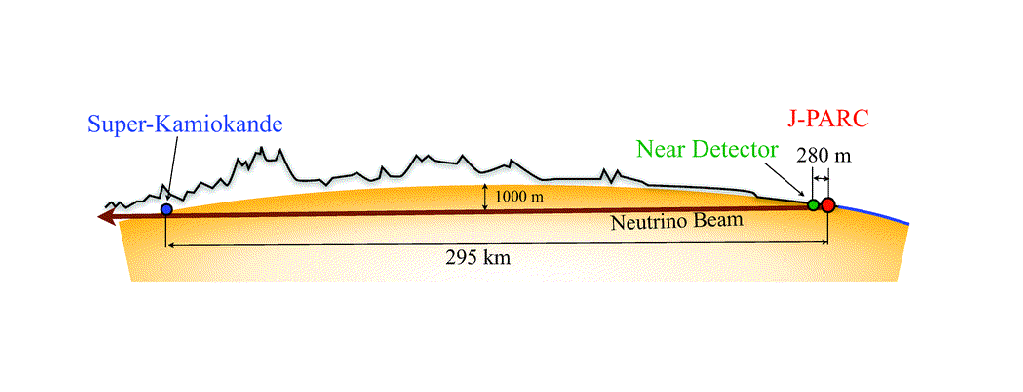
\includegraphics[width=0.98\textwidth]{images/t2k/journey_of_T2K_Neutrino-5.eps}
  \caption[Overview of the T2K experiment]{Overview of the
    \Gls{TK} experiment (not to scale). Taken from~\cite{T2K2011}.}
  \label{fig:t2k}
\end{figure}

The Tokai to Kamioka (\Gls{TK}) experiment~\cite{T2K2011}, represented
in Figure~\ref{fig:t2k}, was designed to measure
$\sin^2(2\theta_{13})$ via electron (anti-) neutrino (\gls{nue} and
\gls{anue}) appearance in a muon $\mbox{(anti-)}$ neutrino (\gls{numu}
and \gls{anumu}) beam~\cite{T2K2011}. Neutrino and anti-neutrino
measurements can lead to hints of a possible non-zero
$\sin(\Delta \delta_{\text{CP}})$ which would indicate violation of
Charge Parity (\Gls{CP}) in the lepton sector. This is one of the
remaining parameters of particle physics that has not been measured
yet. \Gls{TK} also measures $\sin^2(\theta_{23})$ via muon (anti-)
neutrino disappearance~\cite{Abe:2017vif}.

To do this, it uses an off-axis neutrino beam and a far detector,
Super-Kamiokande (\Gls{SK}), placed off-axis at $295$~km from the
Japan Proton Accelerator Research Complex (\Gls{JPARC}) and a beam
energy of $600$~MeV, such that the $\nu_\mu$ to $\nu_\mu$
disappearance probability is maximum; the peak energy also coincides
with the energy where the \Gls{CCQE} processes are the most likely to
happen.

Two other detectors (the Interactive Neutrino GRID, \Gls{INGRID} and
the off-axis Near Detector, \Gls{ND}) are located $280$~m away from
the target and are used for beam and cross section measurements.

In all this thesis, unless stated otherwise, the Z direction refers to
the direction between the target and the far detector (with the
positive direction being towards the far detector), the X direction is
the horizontal direction and Y is the vertical direction (positive Y
being upwards).

\section{T2K Beamline}
\label{sec:t2kbeamline}
The neutrino beam is created by impinging 30~GeV protons on a carbon
target at the \Gls{JPARC} facility in Tokai,
Japan~\cite{FluxT2K2013}. This produces pions and kaons that mainly
decay into muons and neutrinos, as can be seen in the listing in
Table~\ref{tab:nudecaymode}. In Figure~\ref{fig:oaeffect}, the beam
spectrum for different off-axis angles of the neutrino beam is shown.
This technique was developed in 1995 at BNL~\cite{AGS1993}.  The main
idea is to use the 2 body decay kinematics of the hadron to predict
the neutrino energy, which comes from considering the energy and
momentum conservations equation of a pion decaying to a neutrino and a
charged lepton:
\begin{equation}
  E_\nu = \frac{m_\pi^2 - m_\mu^2}{2(E_\pi - p_\pi\cos\theta_\nu)}.
  \label{eq:offaxis}
\end{equation}
Assuming that the parents of the neutrino are mainly pions of mass
$m_\pi$, energy $E_\pi$ and momentum $p_\pi$; they decay into a muon
of mass $m_\mu$ and a neutrino of energy $E_\nu$ and angle
$\theta_\nu$ with respect to the pion trajectory.

When one integrates the pion kinematics from the pion energy
distribution, it can be found that the energy distribution of the
neutrinos also becomes more peaked (smaller width of the distribution)
for increasing off-axis. This effect is visible in
Figure~\ref{fig:oaeffect}: increasing the off-axis angle of the
neutrinos reduces the peak energy of the neutrino flux and the width
of the neutrino energy distribution. At \Gls{TK}, the \gls{numu} beam
whose energy is centred at \energy when viewed from an off-axis angle
of \offaxis as seen on Figure~\ref{fig:oaeffect}. This angle was
optimised to maximise the disappearance probability of the muon
neutrino as can be seen in top of Figure~\ref{fig:oaeffect}.

\begin{figure}[ht]
  \begin{center}
    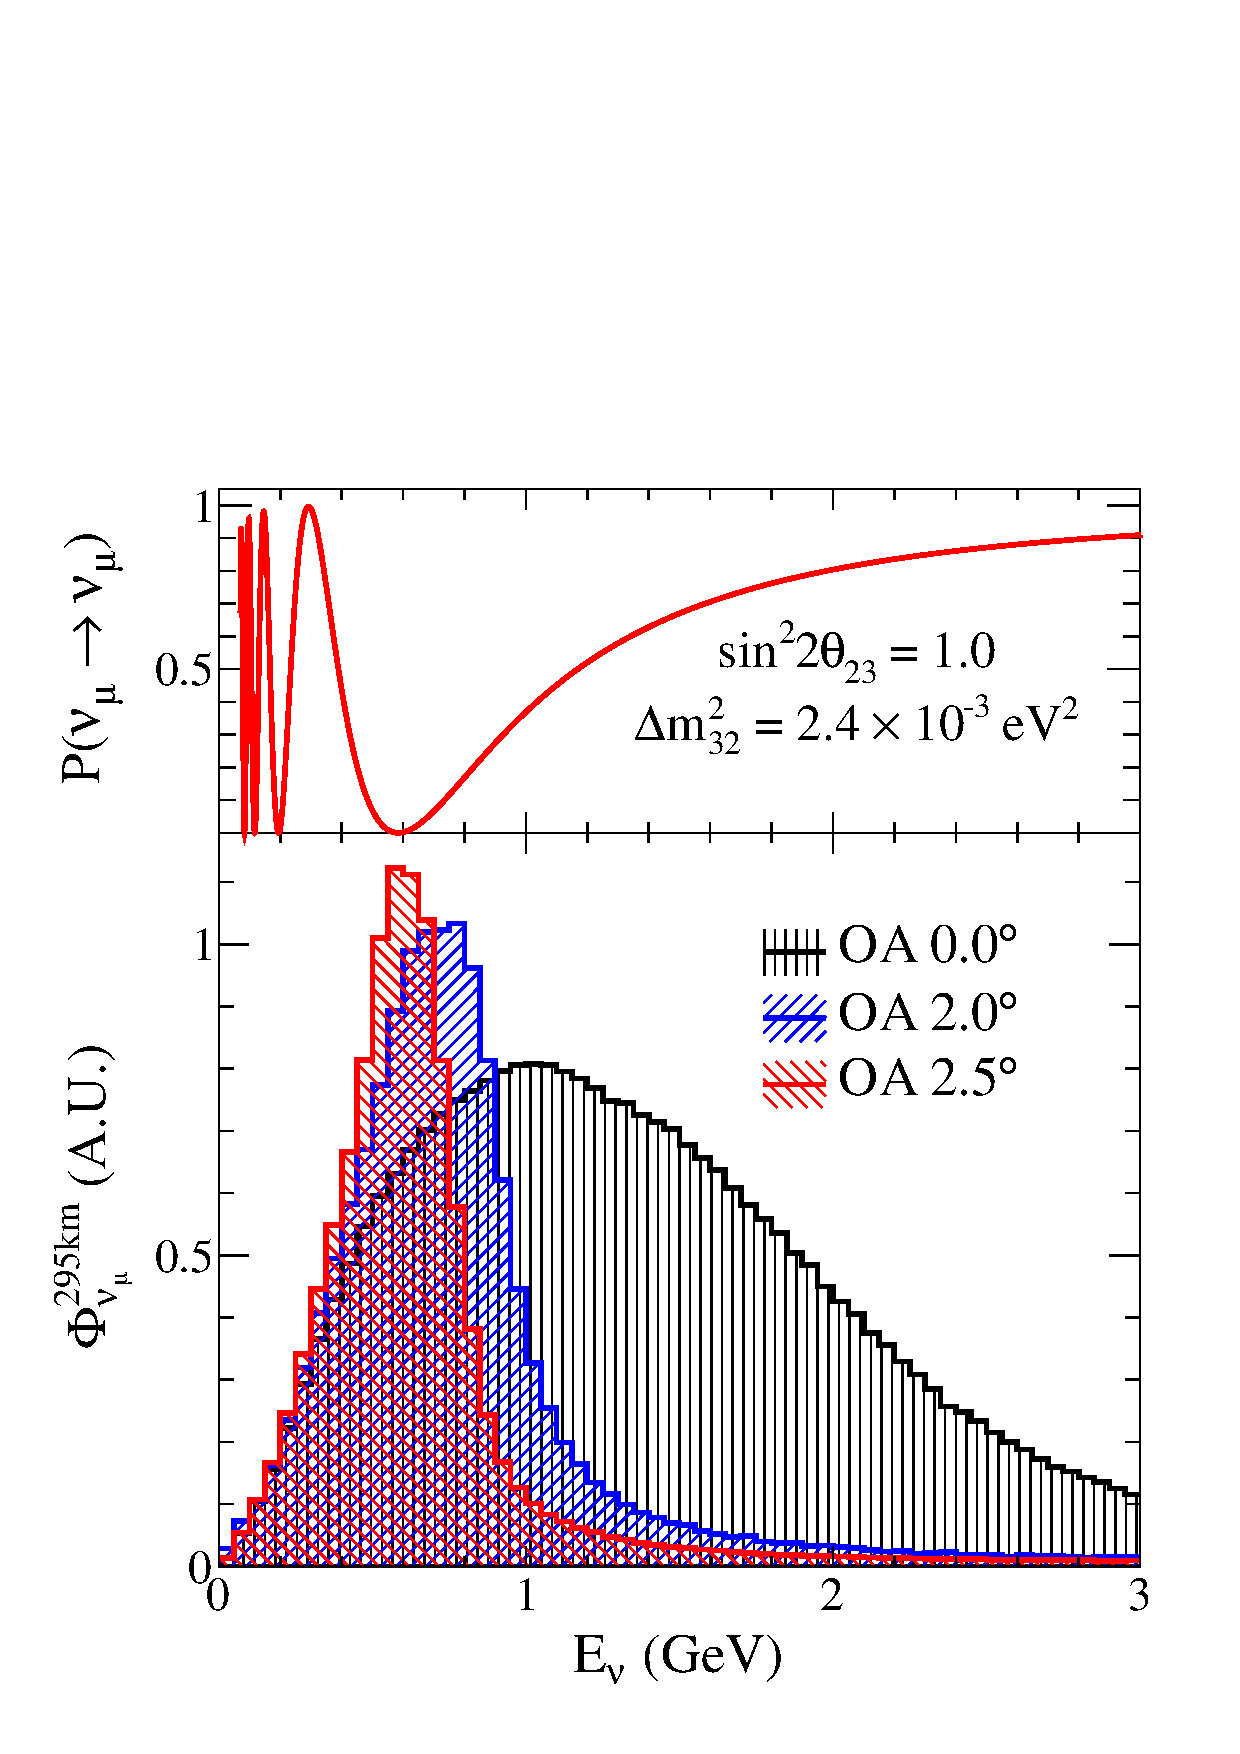
\includegraphics[keepaspectratio=true,width=0.58\textwidth]{images/t2k/oaeffect_flux.pdf}
    \caption[Muon neutrino survival probability assuming maximal
    mixing and $\Delta m^2_{32}=2.4\times 10^{-3}\text{~eV}^2$ at
    SK. Neutrino flux energy distribution for different off-axis at
    295~km]{\textbf{\textit{Top:}} Muon (anti-) neutrino survival
      probability at \Gls{SK} (295~km), against neutrino energy
      assuming maximal mixing ($\sin^22\theta_{23} = 1$) and
      $\Delta m^2_{32}=2.4\times
      10^{-3}\text{~eV}^2$. \textbf{\textit{Bottom:}} \Gls{TK}
      neutrino flux energy distributions for different off-axis
      angles. Taken from~\cite{FluxT2K2013}.}
    \label{fig:oaeffect}
  \end{center}
\end{figure}

\begin{table}[ht]
  \begin{center}
    \begin{tabular}{rlc}
      \toprule
      Particle & Decay products & Branching fraction ($\%$) \\
      \midrule
      $\pi^{+}$ & $\rightarrow \mu^{+}\nu_{\mu}$ & $99.9877$ \\
               & $\rightarrow e^{+}\nu_{e}$ &  $1.23\times10^{-4}$\\
      K$^{+}$ &  $\rightarrow \mu^{+}\nu_{\mu}$ & $63.55$ \\
               &  $\rightarrow \pi^{0}\mu^{+}\nu_{\mu}$ & $3.353$ \\
               &  $\rightarrow \pi^{0}e^{+}\nu_{e}$ & $5.07$ \\
      K$_L^{0}$ & $\rightarrow \pi^{-}\mu^{+}\nu_{\mu}$ & $27.04$ \\
               & $\rightarrow \pi^{-}e^{+}\nu_{e}$ & $40.55$ \\
      $\mu^{+}$ & $\rightarrow e^{+}\bar{\nu}_{\mu}\nu_{e}$ & $100$ \\
      \bottomrule
    \end{tabular}
    \caption[Neutrino-producing decay modes considered in T2K's flux
    simulation]{Neutrino-producing decay modes considered in
      \Gls{TK}'s flux simulation and their branching ratio in
      percentage.  Decay modes for \gls{anumu} and \gls{anue} are
      omitted in this table, but can be derived by taking the charge
      conjugate of the $\pi^{-}$, K$^{-}$ and $\mu^{-}$
      modes. Reproduced from~\cite{FluxT2K2013}.}
    \label{tab:nudecaymode}
  \end{center}
\end{table}

At \gls{JPARC}, the production of the neutrino beam is realised in 3
stages:
\begin{itemize}[noitemsep,topsep=0pt]
\item first, protons are accelerated in the \gls{JPARC} accelerator;
\item then, they are monitored and transported to the target in the
  primary beamline;
\item finally, once the protons hit the target, the hadrons produced
  are propagated in the secondary beamline.
\end{itemize}
The three parts leading to the creation of the neutrino beam are now
described.

\subsection{J-PARC accelerator}
\label{subsec:jparcaccelerator}
The \Gls{JPARC} accelerator consists of one linear accelerator
(\Gls{LINAC}) and two synchrotrons (\Gls{RCS} for Rapid Cycling
Synchrotron and \gls{MR} for Main Ring). The \Gls{LINAC} is 300~m long
and accelerates $H^-$ up to 181~MeV. These $H^-$ are converted to
protons by charge-stripping foils while entering the RCS. The protons
are then accelerated to 3~GeV, and then injected in the \Gls{MR} to be
accelerated to 30~GeV. At this point, 8 bunches are circulating in the
\Gls{MR}, and each of these contains roughly $3\times 10^{14}$
protons.  These 8 bunches are then ``kicked'' (i.e. deviated) by
magnets to go into the primary beamline. This process is repeated
every $2\sim 3$~seconds to create spills.  The time between two
bunches in the same spill is $\sim 600$~ns.  Short spills allow
efficient rejection of cosmogenic particles at the \Gls{ND} and
\Gls{SK}.

\subsection{Primary beamline}
\label{subsec:primarybeam}

\begin{figure}[ht]
  \center
  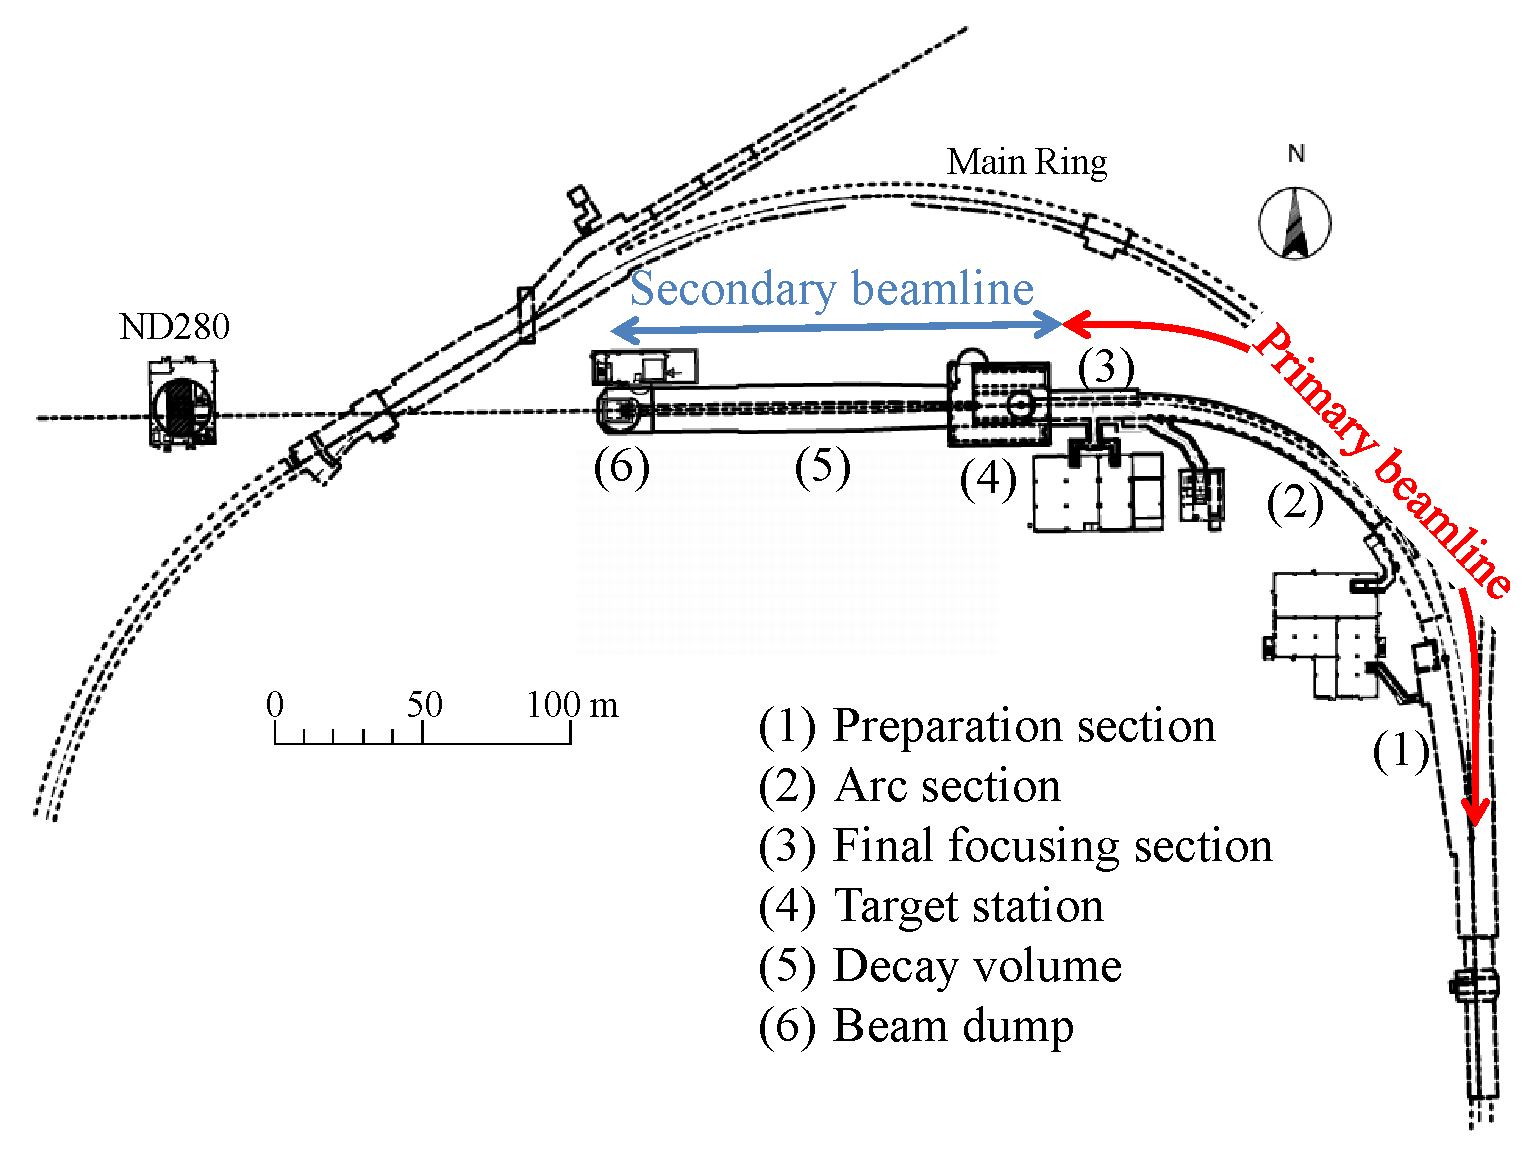
\includegraphics[width=0.6\textwidth]{images/t2k/beamline.eps} \\
  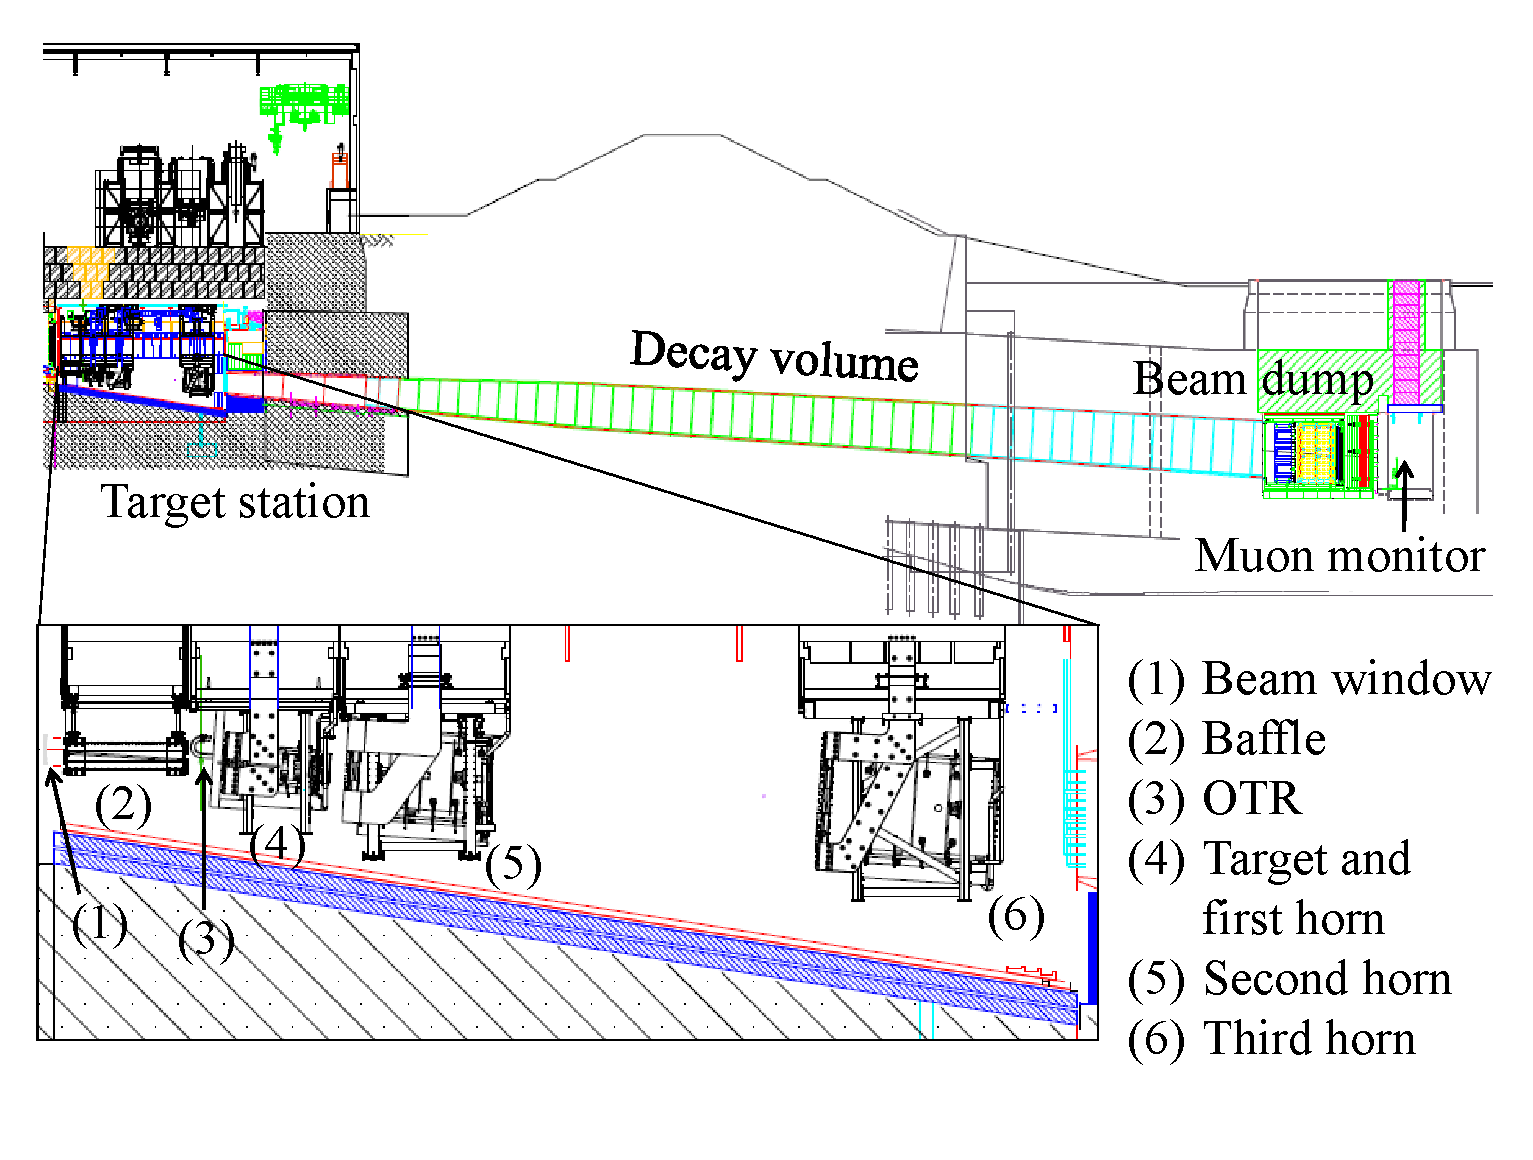
\includegraphics[width=0.6\textwidth]{images/t2k/beamline_sec.eps}
  \caption[Beamline and secondary beamline at
  J-PARC]{\textbf{\textit{Top:}} Beamline at
    \Gls{JPARC}. \textbf{\textit{Bottom:}} Secondary beamline. Taken
    from~\cite{FluxT2K2013}.}
  \label{fig:beamline}
\end{figure}

The whole beamline is represented on the left of
Figure~\ref{fig:beamline}. The primary beamline consists of a
preparation section of 54~m which contains eleven magnets (four
steering magnets, two dipole magnets, and five quadrupole magnets to
focus the beam), an arc-section of 147~m composed of fourteen
superconducting magnets to bend the beam by $\sim 80^{\circ}$, and a
final focusing section (37~m). This last section directs the beam
downwards and focuses the beam on the target; it contains ten magnets
(four steering magnets, two dipole magnets and four quadrupole
magnets).

The primary beamline is instrumented to monitor the proton intensity,
position, profile and losses.

The proton intensity stability measurement is done by five current
transformers (\Glspl{CT}) around the beam. Schematic representation of
a \Gls{CT} is given on the left of Figure~\ref{fig:ssem}.

\begin{figure}[ht]
  \center
  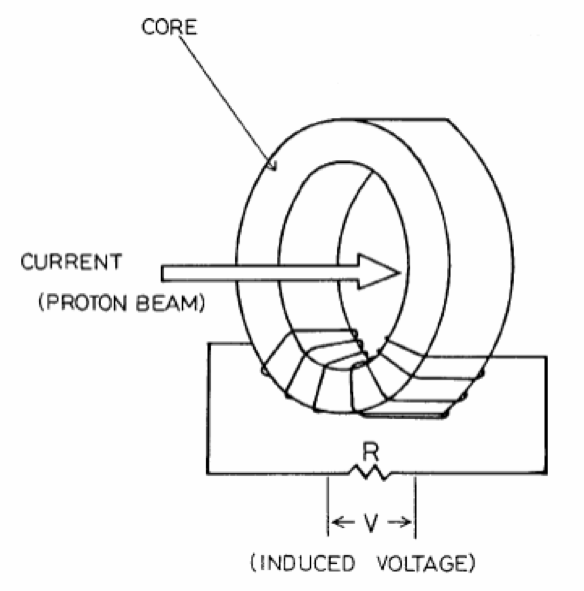
\includegraphics[width=0.6\textwidth]{images/t2k/ct.png} \\
  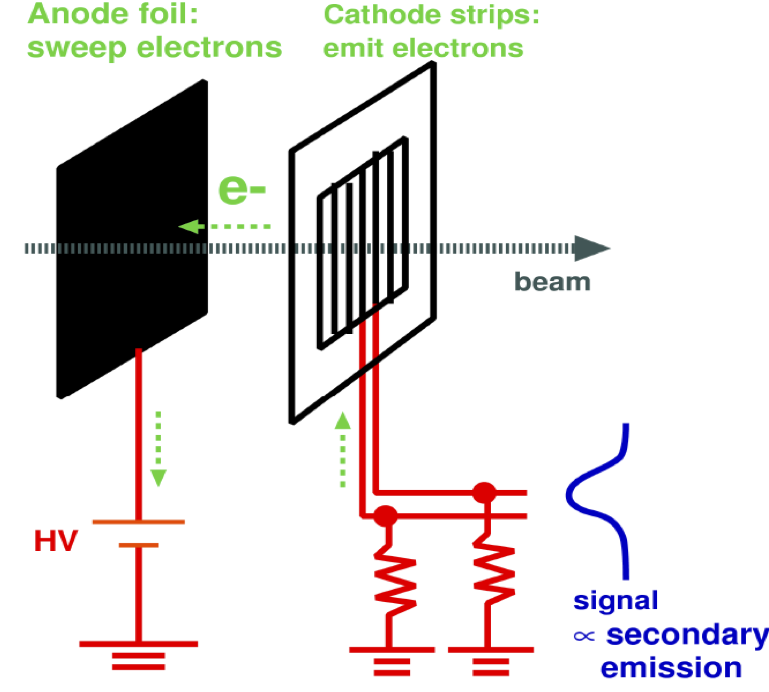
\includegraphics[width=0.6\textwidth]{images/t2k/ssem.png}
  \caption[Illustration of a CT and a SSEM]{\textbf{\textit{Top:}}
    Illustration of a \Gls{CT}. \textbf{\textit{Bottom:}} A
    \Gls{SSEM}. Taken from~\cite{Hartz}.}
  \label{fig:ssem}
\end{figure}

There are fourty Beam Loss Monitors (\Glspl{BLM}), which are gaseous
detectors around the beamline. They are able to detect protons
escaping from the beam which ionise the gas. The \Glspl{BLM} can
trigger an interlock which stops the operations of the beam if the
losses exceed a certain threshold value.

Nineteen \Glspl{SSEM} (Segmented Secondary Emission Profile Monitors)
are located in the beam pipe. They consist of strips oriented in the X
and Y directions placed in front of an anode foil; a bias voltage is
then applied between the strips and the anode. When the beam goes
through, it creates electrons on the strips that are accelerated to
the anode. This process generates a current on each strip directly
proportional to the number of protons crossing it. An illustration of
the device is given on the right of Figure~\ref{fig:ssem}. Because the
\Glspl{SSEM} are destructive of the proton beam and lead to
unacceptable beam loss, they are movable and are only used at specific
times, during the so-called ``beam tuning'' runs. In normal physics
runs, only the last \Gls{SSEM} is used.

Finally, twenty-one \Glspl{ESM} (Electro-Static Beam Position Monitor)
are located near the \Gls{SSEM} to measure the electrostatic shape of
the beam; these are capacitors which give access to the position of
the beam in the beam pipe.

\subsection{Secondary beamline}
\label{subsec:secondarybeam}
The most upstream components of the secondary beamline are in the
target station. It contains the \Gls{OTR} (Optical Transition
Radiation Monitor), which is a device composed of a foil that produces
radiation and fluorescent light when the beam crosses it.  This is
imaged using mirrors and a camera. This device has access to the beam
position and size before it hits the target, 280~mm downstream of it.

The target is a graphite cylinder. Its length is 91.4~cm and its
diameter 2.6~cm. The size and material have been carefully designed to
resist the heat wave generated by the high intensity proton bunches
impinging it. The target is surrounded by an inert helium vessel (15~m
in length, 4~m in width and 11~m in height).

The other parts of secondary beamline are downstream of the carbon
target, i.e. they manipulate and monitor the hadrons produced by the
proton collision on the target. This part is represented on the right
hand side of Figure~\ref{fig:beamline}.

Downstream of the target station, one finds a decay volume for the
hadrons. It is an empty 96~m long steel tunnel, which measures 1.4~m
wide upstream and 3.0~m wide downstream, whereas the height is
increased from 1.7~m to 5.0~m between the upstream and the downstream
part.

Finally, the beam dump is downstream of the decay tunnel. It is used
to stop the muons and the hadrons that have not decayed in the
tunnel. The MUon MONitor (MUMON) is placed just after the beam dump to
detect the muons going through.

Three magnetic horns are placed around the secondary beamline. The
first one is around the target station and serves to collect the
pions. The second and third ones focus the pions. In neutrino mode,
these horns operate at 250~kA and produce a magnetic field of up to
1.7~T (so-called Forward Horn Current, \Gls{FHC}). The current can be
reversed to focus negative pions and produce an anti-neutrino beam
(Reverse Horn Current, \Gls{RHC}). The effect of the horns is to
increase 17-fold the neutrino flux at the far detector. They also
provide better rejection of wrong sign hadrons which produce
background neutrinos for oscillation analysis, making them fundamental
parts of the \Gls{TK} experiment. The beam composition at the off-axis
near detector is shown in Table~\ref{tab:flavor_frac}.

\begin{table}[ht]
  \center
  \tabcolsep=0.11cm
  \begin{tabular}{lccccc}
    \toprule
    \multicolumn{2}{c}{Energy Range [GeV]} & $0$ to $1.5$ & $1.5$ to $3.0$ &  greater than $3.0$ & all \\ 
    \midrule
    Beam mode & Flavour & \multicolumn{4}{c}{Proportion: relative (total)} \\
    \midrule
    \multirow{4}{*}{Neutrino}
                                           & \gls{numu}  & $93.8\%   (84.9\%)$   & $81.7\%  (4.55\%)$   & $88.6\% (3.49\%)$  & $92.9\% $  \\
                                           & \gls{anumu} & $5.23\%   (4.74\%)$   & $14.1\%  (0.784\%)$  & $7.97\% (0.314\%)$ & $5.83\% $  \\
                                           & \gls{nue}   & $0.869\%  (0.786\%)$  & $3.44\%  (0.192\%)$  & $2.8\%  (0.11\%)$  & $1.09\% $  \\
                                           & \gls{anue}  & $0.0852\% (0.0771\%)$ & $0.787\% (0.0439\%)$ & $0.66\% (0.026\%)$ & $0.147\% $ \\
    \midrule
    \multirow{4}{*}{Anti-neutrino}
                                           & \gls{numu}  & $7.07\%  (6.53\%)$  & $32.7\% (1.68\%)$   & $42.4\% (1.09\%)$   & $9.3\% $   \\
                                           & \gls{anumu} & $92\%    (84.9\%)$  & $63.8\% (3.29\%)$   & $53.5\% (1.37\%)$   & $89.5\% $  \\
                                           & \gls{nue}   & $0.131\% (0.121\%)$ & $1.37\% (0.0705\%)$ & $2.07\% (0.0529\%)$ & $0.244\% $ \\
                                           & \gls{anue}  & $0.83\%  (0.766\%)$ & $2.17\% (0.112\%)$  & $1.97\% (0.0505\%)$ & $0.929\% $ \\
    \bottomrule
  \end{tabular}
  \caption[Fraction of the total flux by flavour]{Fraction of the
    total flux by flavour in bins of the neutrino energy when running
    in neutrino mode (run 4) and anti-neutrino mode (run 5) at the
    off-axis near detector (\Gls{ND}). The fractions in parentheses
    are relative to the total flux over all neutrino
    energies. Extracted from the neutrino flux prediction from the
    \Gls{TK} beam group~\cite{TomislavVladisavljevicFluxTuning2017}.}
  \label{tab:flavor_frac}
\end{table}

After simulation and including the constraints from the replica target
measurements at the NA61~/~SHINE
experiments~\cite{Abgrall:2011ae,Abgrall:2011ts,Abgrall:2015hmv}, the
flux uncertainty reaches $\sim8\%$ at the energy peak and the
different components of the flux can be estimated as a function of the
neutrino energy for neutrino and anti-neutrino modes, as can be seen
in Figures~\ref{fig:flux1} and \ref{fig:flux2}. This uncertainty is
expected to decrease as more data from NA61~/~SHINE are analysed.

\begin{figure}[ht!]
  \center
  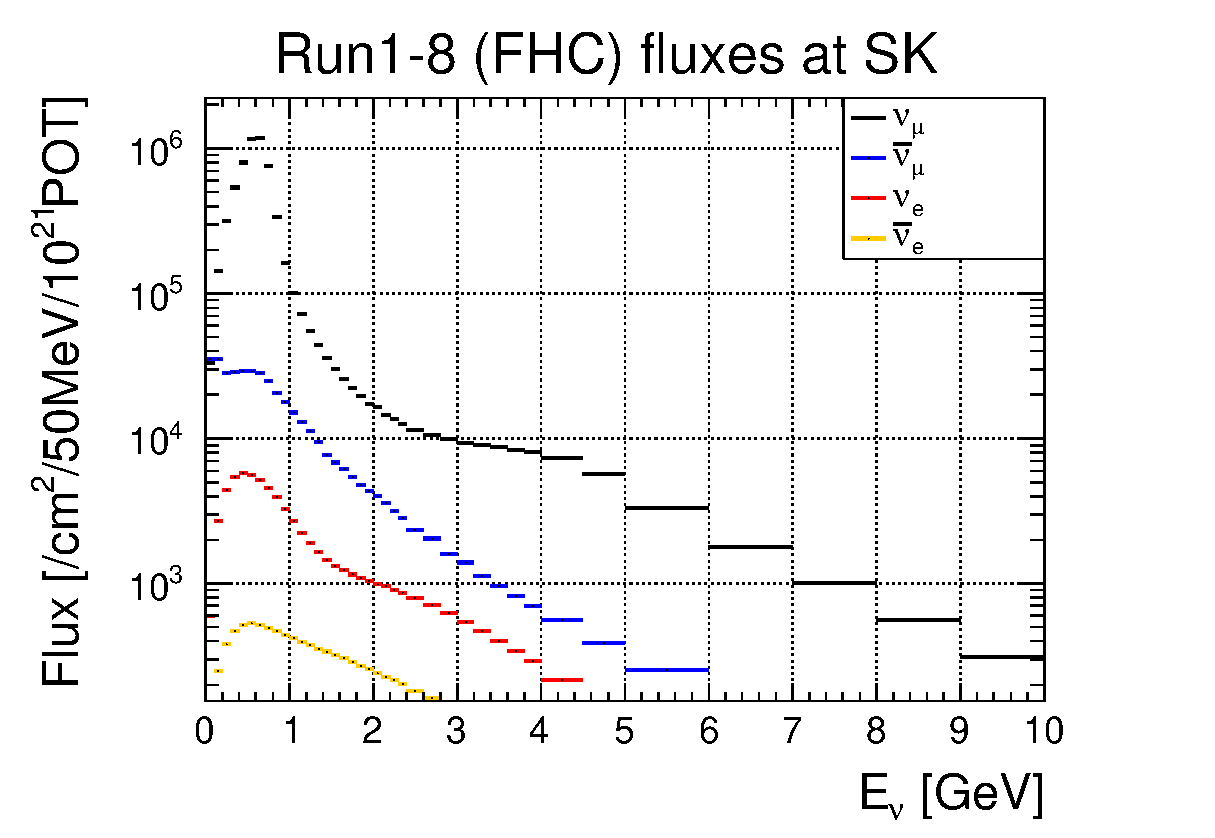
\includegraphics[width=0.6\textwidth]{images/t2k/SK_FHC_flux.eps} \\
  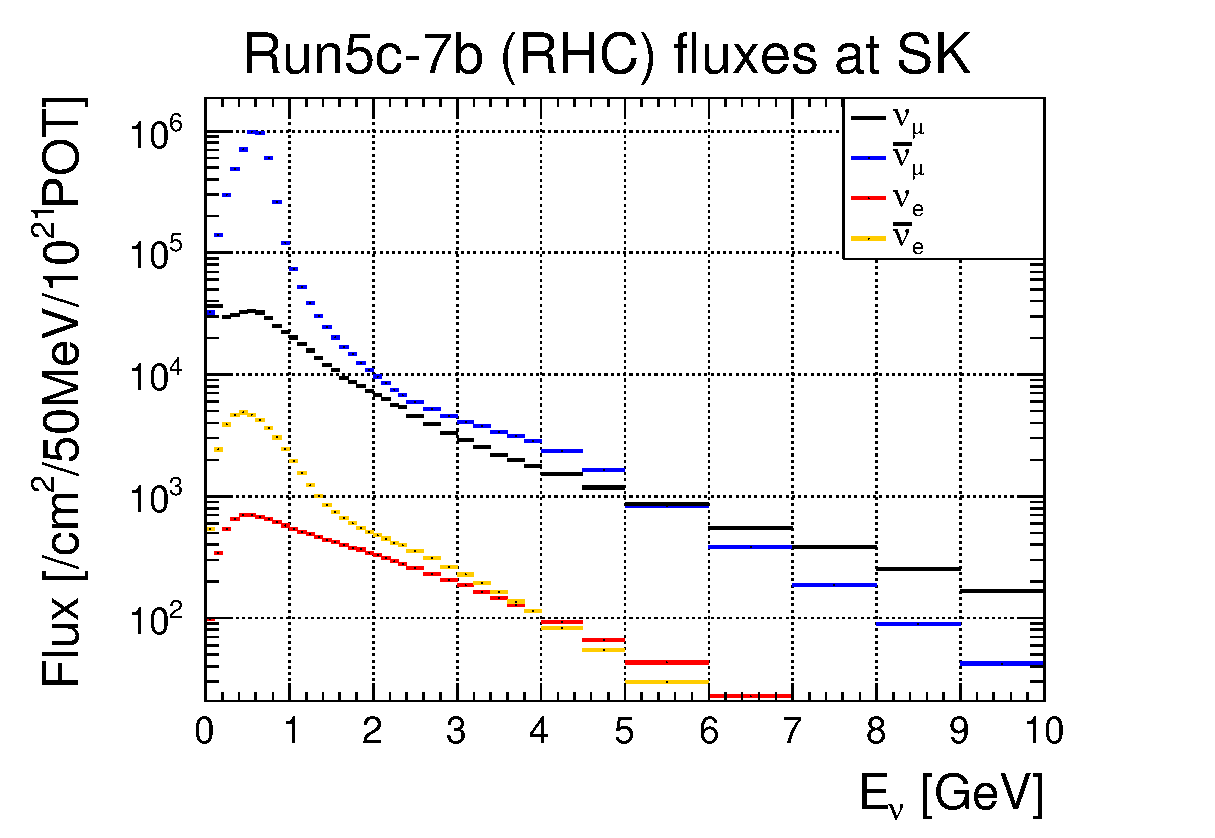
\includegraphics[width=0.6\textwidth]{images/t2k/SK_RHC_flux.eps}
  \caption[Neutrino flux prediction in (anti-) neutrino
  mode]{\textbf{\textit{Top:}} Neutrino flux prediction in neutrino
    mode. \textbf{\textit{Bottom:}} Neutrino flux in anti-neutrino
    mode. Extracted from the neutrino flux prediction and errors from
    the \Gls{TK} beam
    group~\cite{TomislavVladisavljevicFluxTuning2017,MarkHartzFluxUncertainty2017}.}
  \label{fig:flux1}
\end{figure}

\begin{figure}[ht!]
  \center
  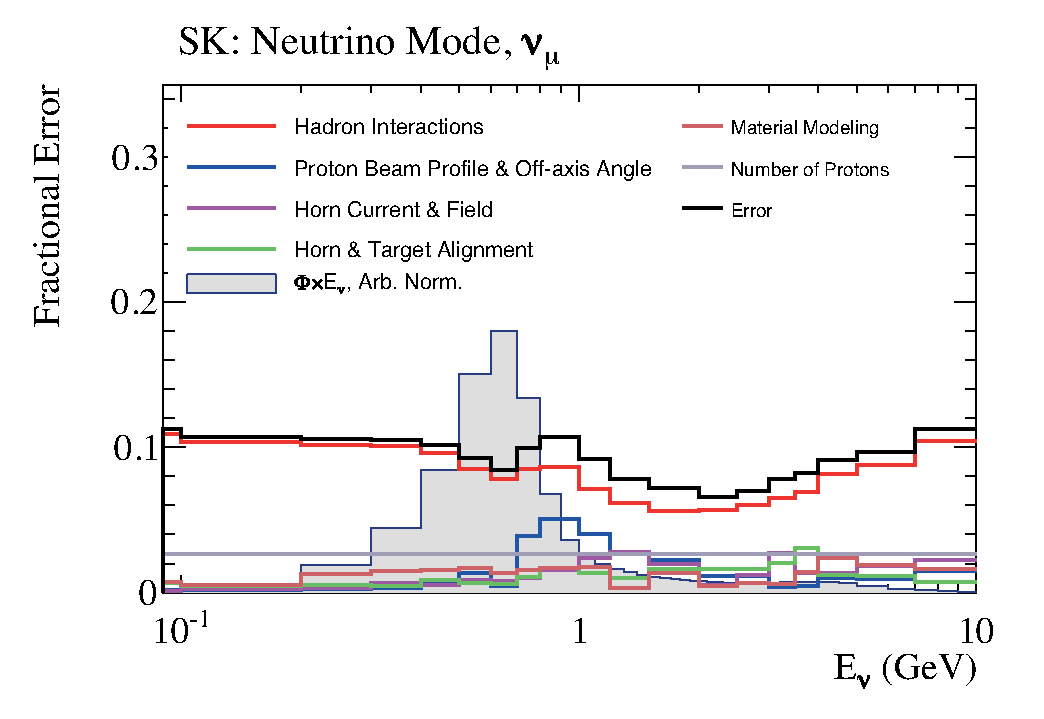
\includegraphics[width=0.6\textwidth]{images/t2k/SK_numode.eps} \\
  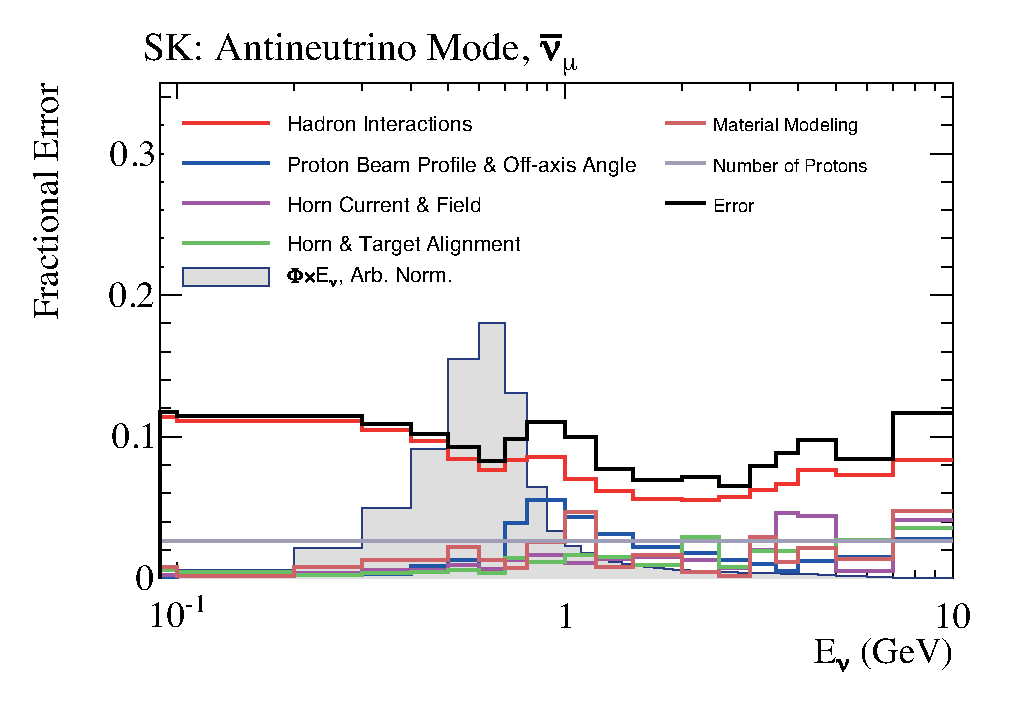
\includegraphics[width=0.6\textwidth]{images/t2k/SK_anumode.eps}
  \caption[Neutrino flux prediction errors in (anti-) neutrino
  mode]{\textbf{\textit{Top:}} Diagonal uncertainties on the
    \gls{numu} flux in neutrino mode at \Gls{SK}, overlaid with the
    neutrino rate (cross section times flux) \textbf{\textit{Bottom:}}
    Diagonal uncertainties on the \gls{anumu} flux in anti-neutrino
    mode at \Gls{SK}, overlaid with the neutrino rate. Extracted from
    the neutrino flux prediction and errors from the \Gls{TK} beam
    group~\cite{TomislavVladisavljevicFluxTuning2017,MarkHartzFluxUncertainty2017}.}
  \label{fig:flux2}
\end{figure}
\clearpage

\section{Near detectors}
\label{sec:neardetectors}
The near detector suite is composed of 2 detectors, \Gls{INGRID} and
\Gls{ND}. Both of them are in the so-called ``pit''
(Figure~\ref{fig:pit}). Their designs are described here.

\begin{figure}[ht]
  \center
  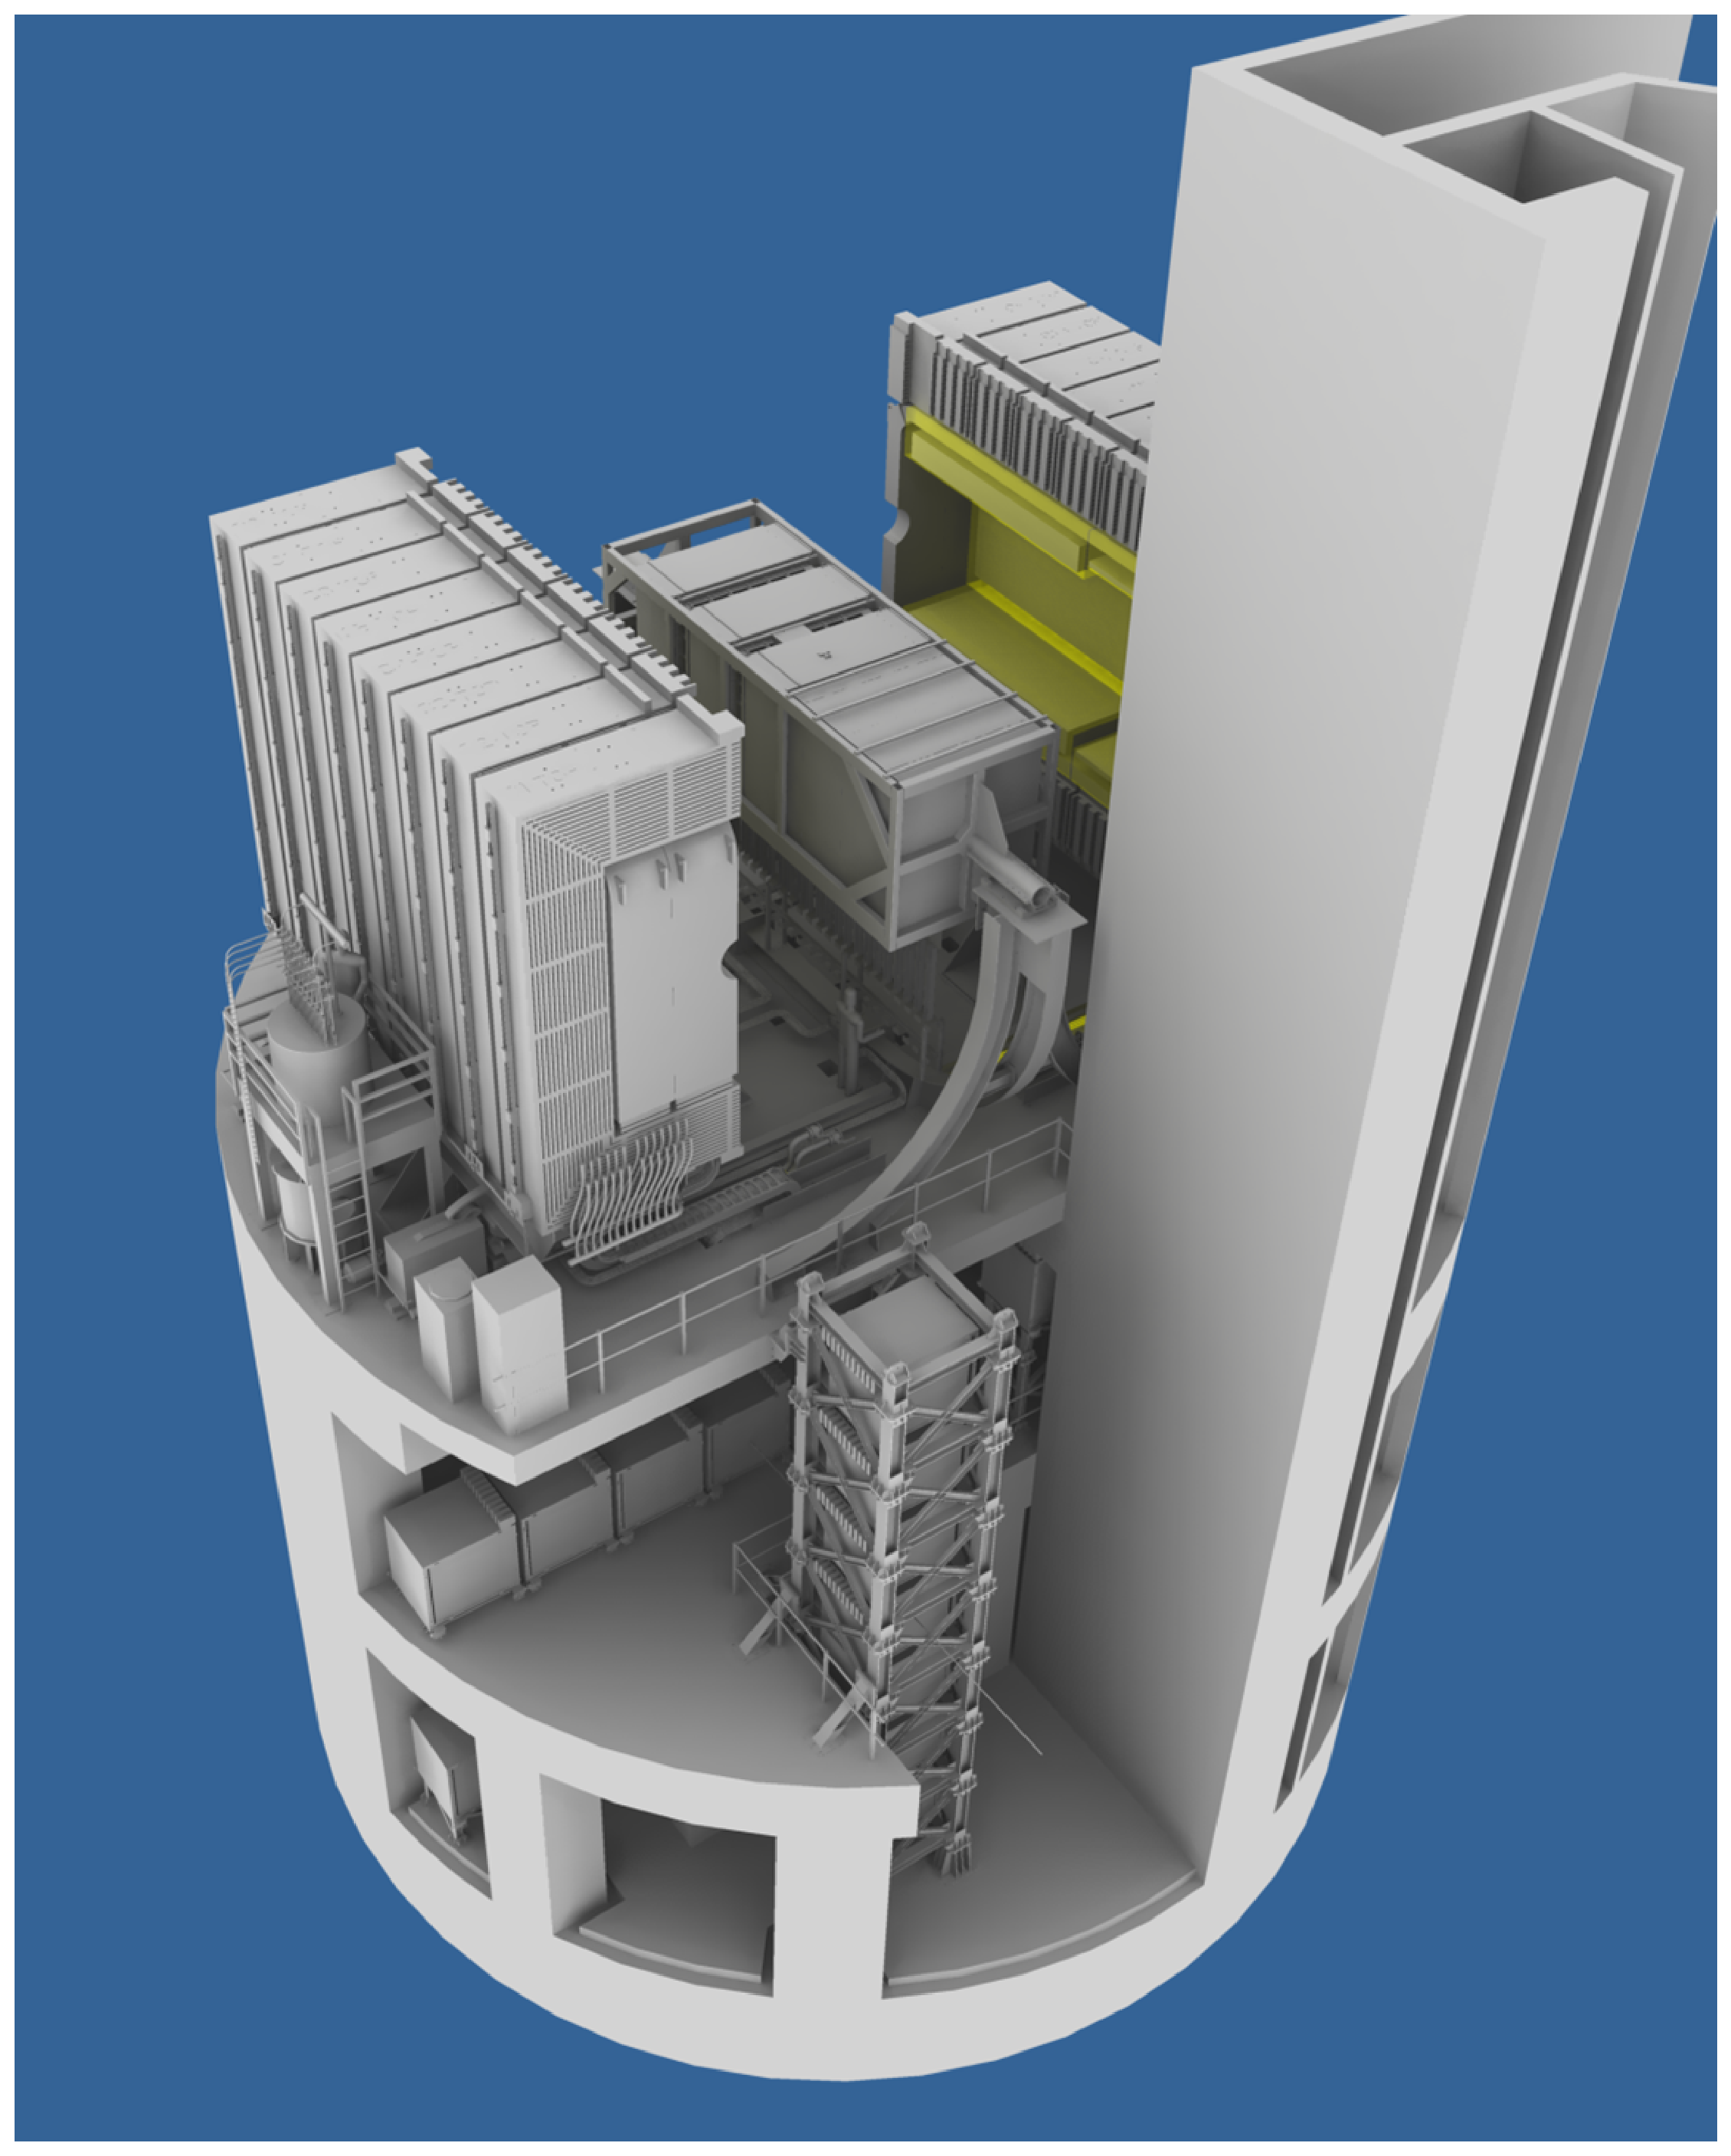
\includegraphics[width=0.48\textwidth]{images/t2k/ND280Pit.eps}
  \caption[Near detector complex]{Near detector complex of the
    \Gls{TK} experiment. On the top, the off-axis near detector at 280
    metres (\Gls{ND}) can be seen in open configuration; in the
    bottom, the Interactive Neutrino GRID (\Gls{INGRID}) cross
    structure can be seen. Taken from~\cite{T2K2011}.}
  \label{fig:pit}
\end{figure}

\subsection{Interactive Neutrino GRID}
\label{subsec:ingrid}
The \Gls{INGRID} (Interactive Neutrino GRID) detector is composed of
sixteen modules. They are placed in a cross structure as shown in
Figure~\ref{fig:INGRID}. The centre of the cross corresponds to the
centre of the beam. \Gls{INGRID}'s primary purpose is to monitor the
beam centre. A 10~cm precision is required to get a 0.4~mRad precision
in the direction of the beam which is an important input to know the
peak energy as shown earlier in Equation~\ref{eq:offaxis}.

\begin{figure}[ht]
  \center
  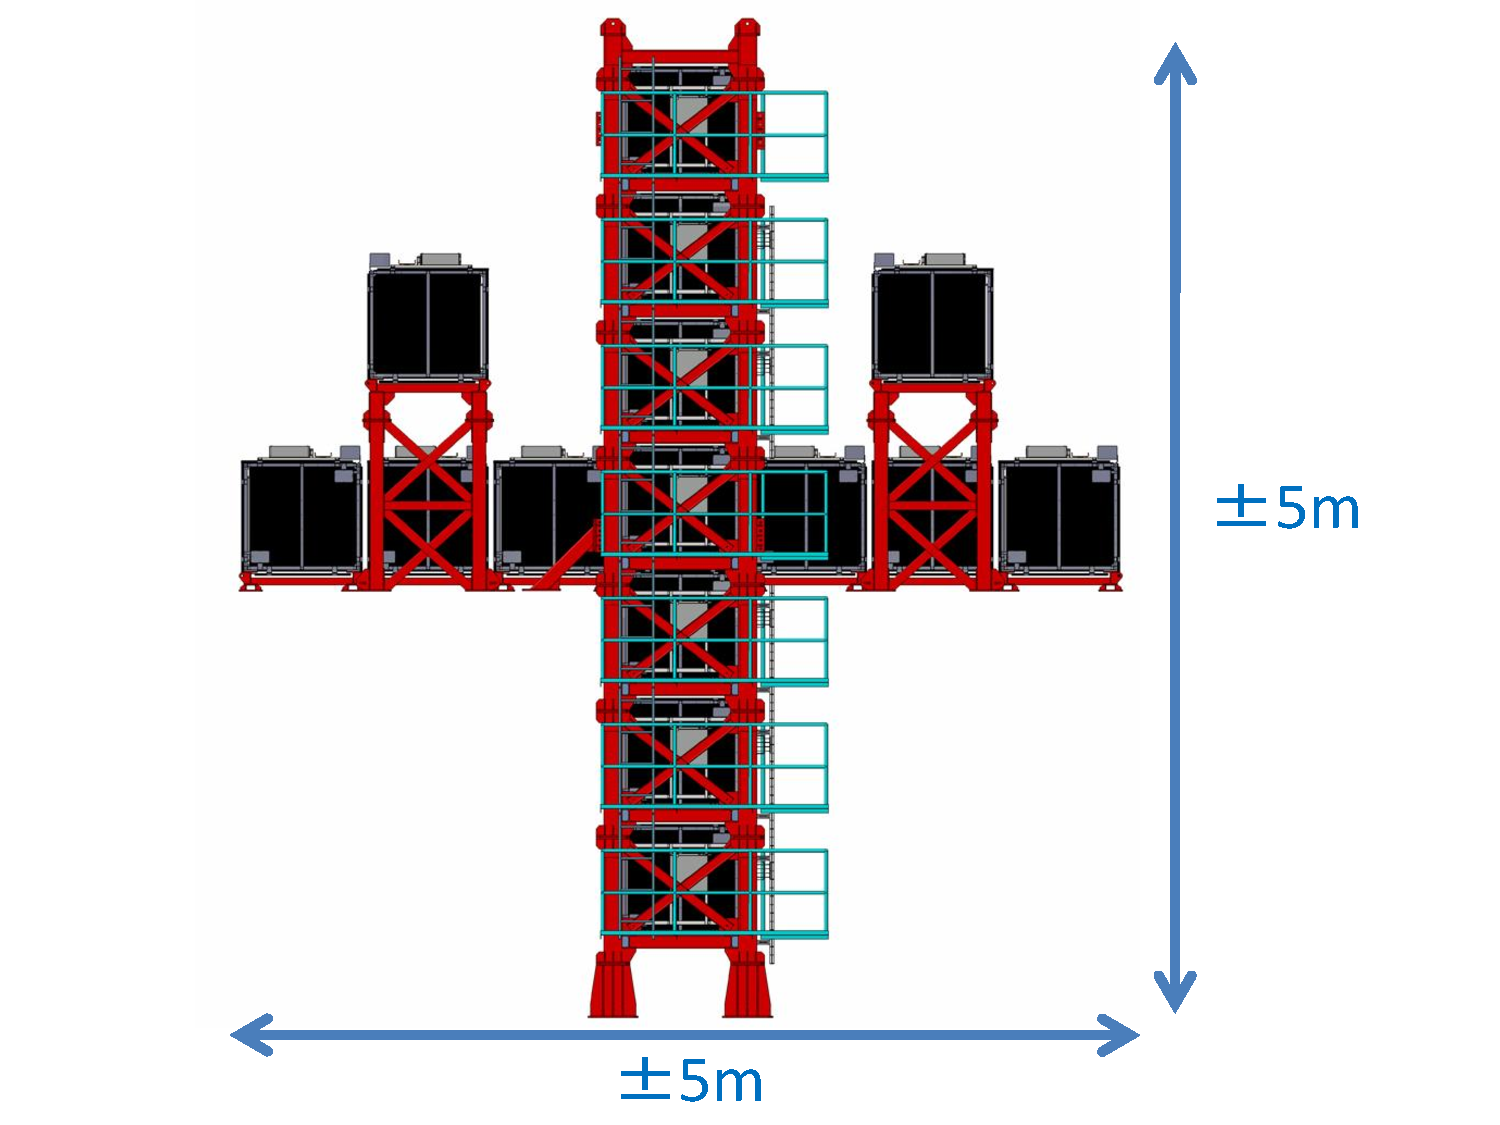
\includegraphics[width=0.48\textwidth]{images/t2k/ingrid.pdf}
  \caption[INGRID detector]{\Gls{INGRID} detector of the \Gls{TK}
    experiment. Taken from~\cite{T2K2011}.}
  \label{fig:INGRID}
\end{figure}

All the modules have the same design. They consist of nine iron layers
of $124 \times 124 \times 6.5\text{~cm}^{3}$ providing a total target
mass of 7.1~t for each module. These iron layers are alternated with
eleven scintillator layers.  Each one of these layers is made with
forty-eight bars oriented both in X and Y directions (perpendicular to
the beam axis). This cube is surrounded by a veto region made of
twenty-two scintillator bars oriented in the Z direction. All the
scintillators have a wavelength shifting fibre (\Gls{WSF}) going
through the centre to collect the light produced by the particles. The
scintillators are made of polystyrene doped with \Gls{PPO} and
\Gls{POPOP} (which emits UV light from charged particle and shifts the
light frequency to enhance the light absorption on the fibre,
respectively). They have a rectangular cross section of
$1.0 \times 5.0\text{~cm}$ and are co-extruded with reflective
material ($TiO_2$) to reflect escaping photons, thus reducing
cross-talk between bars and enhancing the photon collection yield on
the fibre.

In addition, a ``proton module'' was designed to study the protons
from \gls{numu} interactions. The difference with the other module is
that it has finer scintillator bars and no iron layer, which improves
the tracking capabilities for short proton tracks. It is located
between the two central modules.

The readouts were provided by the Hamamatsu company. They are
Multi-Pixel Photon Counters (\Glspl{MPPC}). These photosensors are
connected to the \Gls{WSF} which collects the light inside the
scintillators. This set-up provides the timing and the detected light
which are used to reconstruct the particles' trajectories, charge and
momentum.

\subsection{Multi-Pixel Photon Counter}
\label{subsec:mppc}
The Mutli-Pixel Photon Counters (\Glspl{MPPC}\footnote{\Gls{MPPC} is a
  trademark of Hamamatsu Photonics, the \Glspl{MPPC} used at the
  \Gls{TK} are the model S10362-13-050C~\cite{MPPC}.}, also referred
as Silicon photo-multiplier, \Gls{SiPM}) are elementary parts of the
near detectors at \Gls{TK}. They are used in all the scintillator
detectors and are the readout for the photons from the
\Gls{WSF}\footnote{of reference: Kuraray Y11 (200) S-35
  J-type~\cite{T2K2011}.}. A single \Gls{MPPC} measures
$1.3\times 1.3 \text{~mm}^2$ and contains 667 individual pixels. The
\Gls{MPPC} pixels are avalanche photodiodes.

In the Geiger regime, which is the one the \Gls{MPPC} are opperated
at, the output charge of the diode does not depend on the number of
the photoelectrons that have fired the pixel, and the output charge is
given by the simple relation:
\begin{equation}
  Q=C(V-V_{\text{BD}}),
\end{equation}
where $Q$ is the output charge, $C$ ($\simeq60\text{pF}$) is the
internal capacity of the diode and $V$ is the applied bias voltage and
$V_\text{BD}$, the breakdown voltage, which is around $70\text{V}$.
This set-up gives a gain of about $10^5\sim 10^6$ (nominally
$7.5\times 10^5$). Note that the breakdown voltage is dependent on the
ambient temperature (typically $50\text{~mV}/^\circ\text{C}$), so a
change of few degrees can significantly modify the gains. The value of
the gain has to be calibrated for each period of roughly constant
temperature.

Since the pixels have a binary response (0 or 1 depending if the pixel
was hit), this allows to count photo-electrons depending on the number
of fired pixels. The charge deposited in the scintillator bar is
roughly proportional to the number of pixels hit.

\subsection{Off-Axis Near Detector at 280 meters}
\label{subsec:nd280}
\begin{figure}[ht]
  \center
  \begin{overpic}[width=0.6\linewidth]                {./images/t2k/ND280Exploded-Text-White.eps}
    \put(55,55){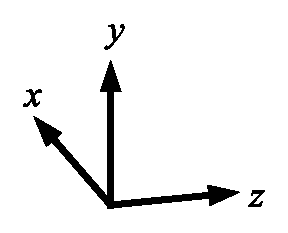
\includegraphics[width=0.12\linewidth]{./images/t2k/ND280-Coord-xyz.eps}}
    \put(0,20) {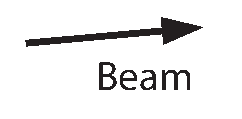
\includegraphics[width=0.1\linewidth ]{./images/t2k/ND280-Coord-Beam.eps}}
  \end{overpic}

  % 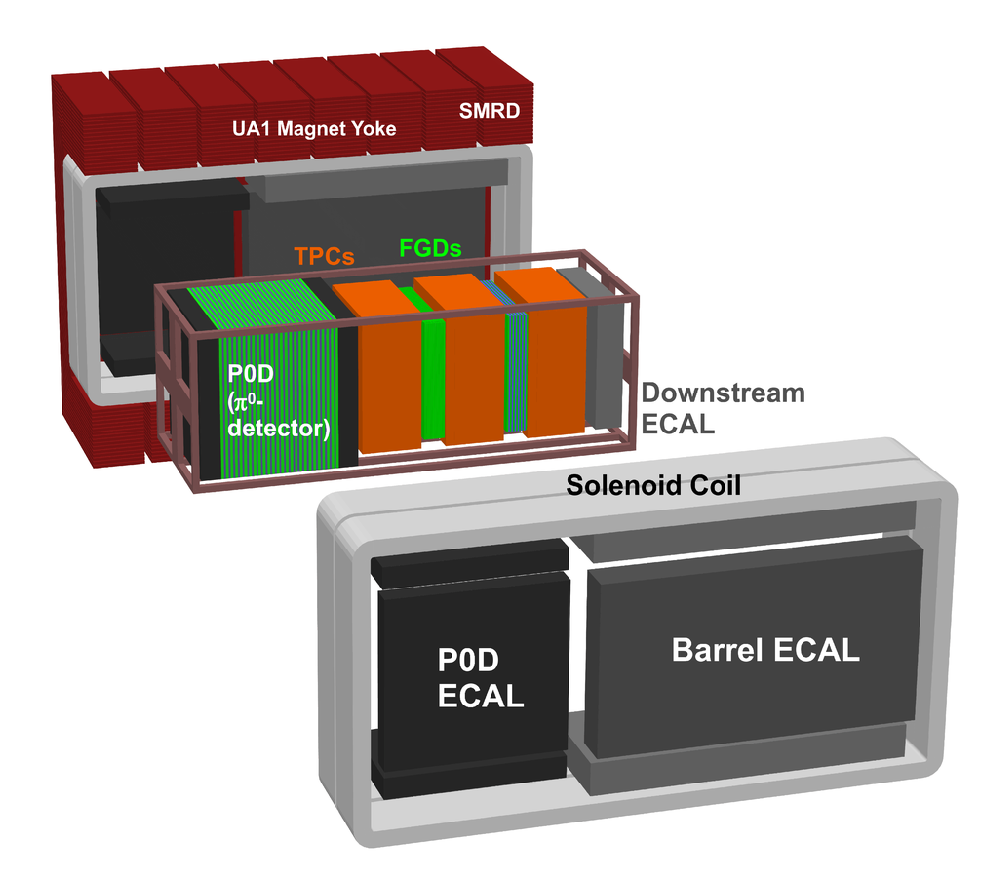
\includegraphics[width=0.68\textwidth]{images/t2k/ND280Exploded-Text-White.eps}
  \caption[Exploded view of the ND280]{Exploded view of the \Gls{ND}
    of the \Gls{TK} experiment, with its coordinate system and beam
    direction. Taken from~\cite{T2K2011}.}
  \label{fig:nd280}
\end{figure}

The off-axis Near Detector at 280 metres (\Gls{ND}), which is used in
the analyses described in this thesis, is a composite detector
enclosed in a magnet. The \Gls{ND} is illustrated on
Figure~\ref{fig:nd280}. It is placed at a $2.5^{\circ}$ off-axis angle
to have the closest neutrino energy distribution to the one in the far
detector. The description of the detector is made from the most
outward to inward regions and upstream to downstream, where upstream
refers to closest position to the target (left of
Figure~\ref{fig:nd280}).

\subsubsection{UA1 Magnet}
\label{subsubsec:magnet}
The magnet consists of aluminium coils circulating around the \Gls{ND}
as can be seen in light grey on Figure~\ref{fig:nd280}. They create a
horizontal dipole field of $0.2$~T. The return yoke (in red) and coils
were reused from the UA1 and the \Gls{NOMAD} experiments at CERN. The
yoke is composed of 2 C-shaped half yokes, that provide magnetic
insulation for the surrounding of the detector. The yoke is used as a
muon spectrometer and contain the magnetic field inside the inner
region of the detector due to their low saturation field. Both halves
are placed on rails that open to allow reach of the inner region. This
is visible in Figure~\ref{fig:pit}.

The magnetic field is a central part in the particle identification
with the Time Projection Chambers as will be shown later, so the field
was carefully calibrated in the whole detector before the inner parts
of the detector were placed inside it.

\subsubsection{Side Muon Range Detector}
\label{subsubsec:smrd}
The Side Muon Range Detector (\Gls{SMRD})~\cite{SMRD} is placed inside
the yoke and can identify escaping muons from neutrino interactions
inside the inner detector. It also serves as veto (or trigger) for
cosmic muons.  It is composed of 2008 scintillator bars with coarse
granularity ($7 \times 175 \times 875 \text{mm}^{3}$) oriented
horizontally and vertically.

\subsubsection{Pi~Zero Detector}
\label{subsubsec:p0d}
The Pi~Zero detector (\Gls{PD})~\cite{POD} is a scintillator detector
that was designed to measure the neutrino cross section of neutral
pion (\gls{piz}) production on water. As scintillator offers better
resolution than water, the idea is to have bags that can be filled
with water between the scintillator bars. One can make two
measurements: one with water in the bag and another one without
water. Both measurements can be used simultaneously to get a cross
section on water only.

The \Gls{PD} is made of fourty modules each containing 134 vertical
and 126 horizontal scintillator bars, alternating with brass as
depicted on Figure~\ref{fig:pod}. This set-up is realised to damp the
\Gls{EM} showers. The scintillator bars have very similar design to
the ones in the \Gls{INGRID} detector (\Gls{PPO} and \Gls{POPOP}
doped, coated with $TiO_2$, using a \Gls{WSF} and \Gls{MPPC} readout),
except their triangular cross section as can be seen in the insert of
Figure~\ref{fig:pod}. Their sizes are 33~mm at the base of the
triangle, 17~mm for the height, similarly to what was done for the
\Gls{MINERVA} neutrino experiment.

In the upstream and downstream parts of the \Gls{PD}, the water is
replaced by iron to contain the Electro-Magnetic (\Gls{EM}) showers.

\begin{figure}[ht]
  \center
  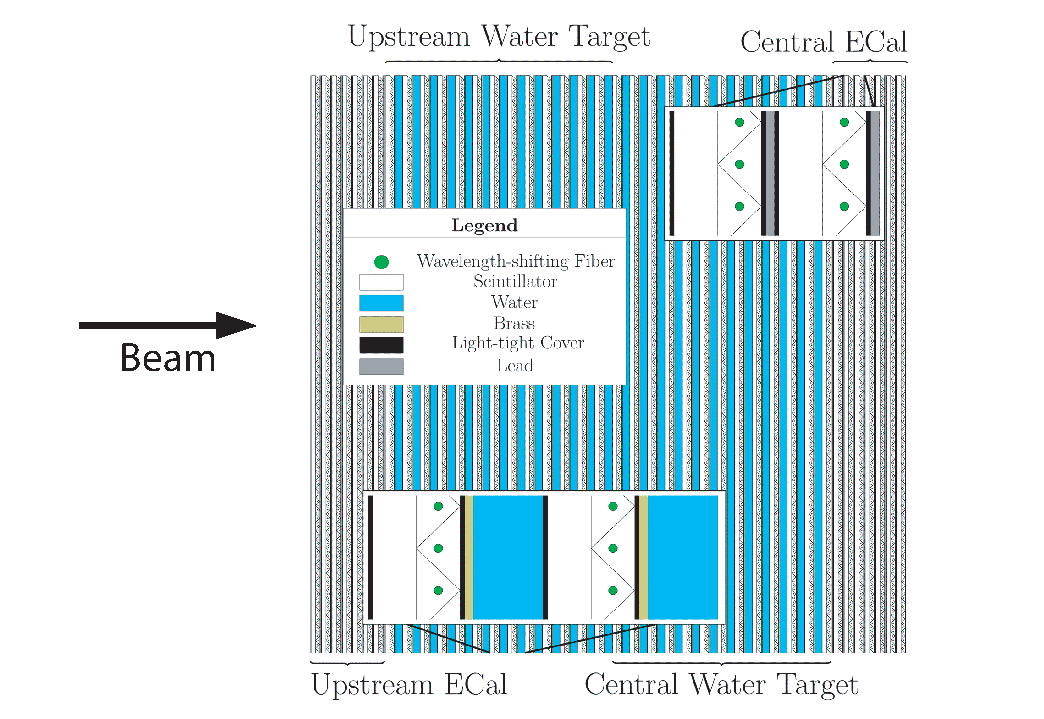
\includegraphics[width=0.6\linewidth]{images/t2k/p0d-schematic.eps}
  \caption[P0D of the ND280]{\Gls{PD} of the \Gls{ND} at the \Gls{TK}
    experiment. The neutrino beam is directed from the left to the
    right. Taken from~\cite{POD}.}
  \label{fig:pod}
\end{figure}

\subsubsection{Time Projection Chambers}
\label{subsubsec:tpc}
Going downstream from the \Gls{PD}, one finds the first Time
Projection Chambers (\Glspl{TPC})~\cite{TPC}. There are three
\Glspl{TPC} in what is loosely called the tracker region (composed of
the Fine Grained Detectors (\Glspl{FGD}) and \Glspl{TPC} region) of
the \Gls{ND}.

In the central part of the \Gls{TPC}, a cathode is polarised with a
strong negative voltage (-25~kV) which provides a drift field of
275~V/cm across the inner box.

The \Glspl{TPC} are filled with a mix of argon, $CF_4$ and
$i C_4H_{10}$ gas (where the $i$ stands for the ``iso'' isomer, which
means the molecule has a pyramidal configuration) at atmospheric
pressure.  This choice of pressure is to reduce the strains and
deflections on the side panels of the \Glspl{TPC}, as this would
distort the drift electric field in the chamber.  When a charged
particle enters the detector, it ionises the gas and the electrons,
typically a hundred electrons per cm are created in the gaseous argon
at atmospheric pressure. These ionisation electrons are drifted to a
charge detector (MicroMegas).  The drift time depends on the density
of the gas and is typically between $10-100~\mu\text{s}$.

The MicroMegas on the walls opposite to the cathode, record the
delayed pattern of the ionisation. A schematic view of a \Gls{TPC} is
shown in Figure~\ref{fig:tpc}. On each wall of the \Gls{TPC},
MicroMegas are aligned in 2 columns of 6 MicroMegas with a vertical
offset to avoid dead zones.  Each MicroMegas is composed of a Micro
Mesh Gaseous detector that amplifies the charge of the drifted
electron by applying a strong electric field ($\sim40\text{~kV/cm}$)
causing an electron avalanche (similar to an avalanche diode). The
MicroMegas amplifies the signal by a factor of about 2000. This gain
is inversely proportional to the pressure of the gas and thus the
current atmospheric pressure. The electrons from the cascade are then
read in the MicroMegas Pads, which is later called a hit. The size of
a MicroMegas is $342 \times 359 \text{~mm}^2$ and each of them is
meshed in a $36 \times 48$ array of pads, that have sizes of
$6.85 \times 9.65\text{~mm}^2$. This is the typical spatial resolution
for a charged particle crossing the detector.

The argon chamber is surrounded by another gas chamber filled with
carbon dioxide ($CO_2$) to insulate it electrically.

\begin{figure}[ht]
  \center
  %\includegraphics[width=0.6\textwidth]{images/t2k/tpc-eps-converted-to.pdf}
  \caption[Schematic view of the TPC in the ND280]{Schematic view of
    the \Gls{TPC} in the \Gls{ND}. Taken from~\cite{TPC}.}
  \label{fig:tpc}
\end{figure}

The \Gls{TPC} is a very precise detector that can be used for pointing
the particles and measuring their momentum in the magnetic field and
Particle IDentification (\Gls{PID}) by measuring the energy loss along
the trajectory ($dE/dx$) of the particle from the local curvature of
the trajectory in the magnetic field. This is visible in
Figure~\ref{fig:tpcdedx}, which shows the $dE/dx$ of the several
particles (positrons, anti-muons, positively charged pion and proton)
as measured in the \Gls{TPC} against their momentum.

\begin{figure}[ht]
  \center
  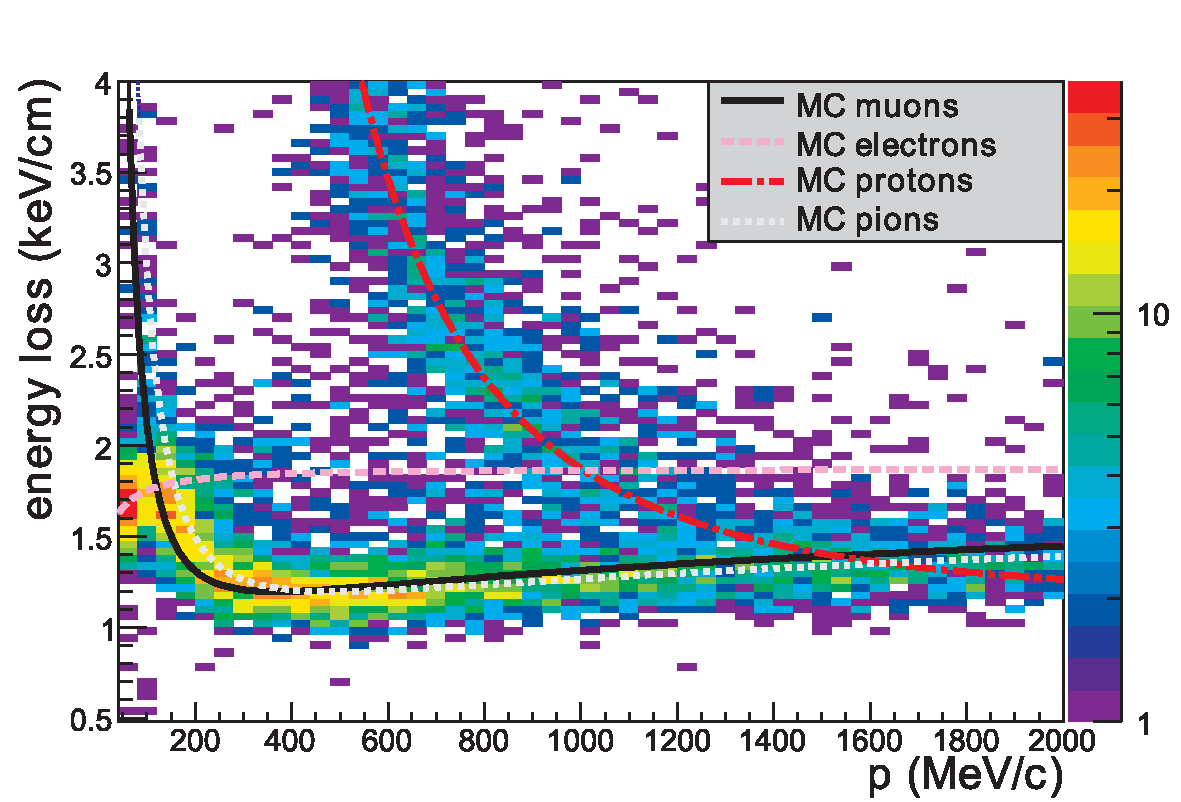
\includegraphics[width=0.6\textwidth]{images/t2k/dedx.pdf}
  \caption[TPC $dE/dx$ distributions for positively charged
  particles]{\Gls{TPC} $dE/dx$ for different ionising particles of
    positive charge in the \Gls{TPC}. Taken from~\cite{TPC}.}
  \label{fig:tpcdedx}
\end{figure}

\subsubsection{Fine Grained Detectors}
\label{subsubsec:fgd}
There are two Fine Grained Detectors (\Glspl{FGD})~\cite{FGD} in the
\Gls{ND}; they are placed in between the \Glspl{TPC}. Each \Gls{FGD}
is composed of scintillator bars which have small cross sections
($9.61 \times 9.61 \times 1864.3 \text{~mm}^3$). They are oriented in
the X and Y directions, alternately. Each scintillator bar has a
\Gls{WSF} in it and a \Gls{MPPC} associated at one end. It has the
same characteristics as those of the \Gls{INGRID} or \Gls{PD}.

When a Minimum Ionising Particle (\Gls{MIP}) enters one bar of the
\Gls{FGD}, it produces generally between ten to thirty photons. Most
of these enter the \Gls{WSF} and reach the \Gls{MPPC}. The
\Glspl{MPPC} amplifies the signal with a gain of about
$5\times 10^{5}$ to create a detectable charge.

Each of the thirty layers is composed of 192 bars, providing active
carbon target of 1.1~t. For the second \Gls{FGD}, six layers were
removed and filled with water to allow neutrino water cross section
measurement similar to what was described in \Gls{PD} section.

\subsubsection{Electromagnetic Calorimeter}
\label{subsubsec:ecal}
The whole \Gls{ND} tracker region (composed of the three Time
Projection Chambers and two Fine Grained Detectors) is surrounded by
an Electromagnetic Calorimeter (\Gls{ECal})~\cite{ECal}. This detector
was designed to measure \gls{piz} coming from neutrino interaction
inside the tracker region.

The \Gls{ECal} is composed of six modules surrounding the tracker
(\Gls{BrECal}, for barrel \Gls{ECal}) parallel to the Z direction, six
modules surrounding the \Gls{PD} (\Gls{P0DECal}) and another placed
after the third \Gls{TPC} (Downstream \Gls{ECal}, \Gls{DsECal}).  All
the \Gls{ECal} modules are made of scintillator bars. These bars have
a cross section of $4.0 \times 1.0 \text{~cm}^2$ and have with similar
specifications as the \Gls{PD}, \Gls{FGD} and \Gls{INGRID} bars. The
scintillator bars are alternated with lead layers to develop the
showers.

The \Gls{DsECal} is composed of thirty-four layers of lead alternated
with fifty layers of scintillator bars oriented in X and Y
directions. A similar design was made for the \Gls{BrECal}, with
thirty-one layers of lead.

The \Gls{P0DECal} is different because of the \Gls{PD} size and the
available space in the UA1 magnet. It only has five layers of lead and
six active layers of scintillator, all of which are oriented in the
same direction.

The \Gls{BrECal} and \Gls{DsECal} have an interaction length allowing
containment of all the showers
($\sim 10\text{X}_0$\footnote{$\text{X}_0$ is defined as the length
  for which an electron~/~photon has $sim 63\%$ chance to
  interact. This length is normalised by the density of the material
  its units are $\text{g} / \text{cm}^2$.}) whereas the \Gls{P0DECal}
cannot contain some of the showers due to its reduced size
($3.6 \text{X}_0$). The \Gls{P0DECal} was designed to veto external
particles.

Note that the \Gls{BrECal} and the \Gls{P0DECal} were placed in the
detector at the start of the run 2 of \Gls{TK}, over the summer 2011.


\section{The far detector: Super-Kamiokande}
\label{sec:sk}
The far detector (SuperKamiokande, \Gls{SK}) is located at 285~km away
from the graphite target at \Gls{JPARC}, in the Kamioka mine, on the
western cost of Japan~\cite{SK2003}. The mine is 1,000~m deep, under
the mount Ikenoyama, which is equivalent to roughly
2,700~m.w.e. (metre equivalent water).

The geometry of the detector is cylindrical (vertically), and the
vessel is made of stainless steel. A diagram of the detector is shown
in Figure~\ref{fig:sk}.  \Gls{SK} is composed of two coaxial cylinders
that define the inner volume and the outer volume. The inner detector
has a diameter of 33.8~m and the outer detector is 2~m wide. Its
height is 36.2~m. This provides a fiducial volume of 22.5~kton of
ultra-pure water.

\begin{figure}[ht]
  \center
  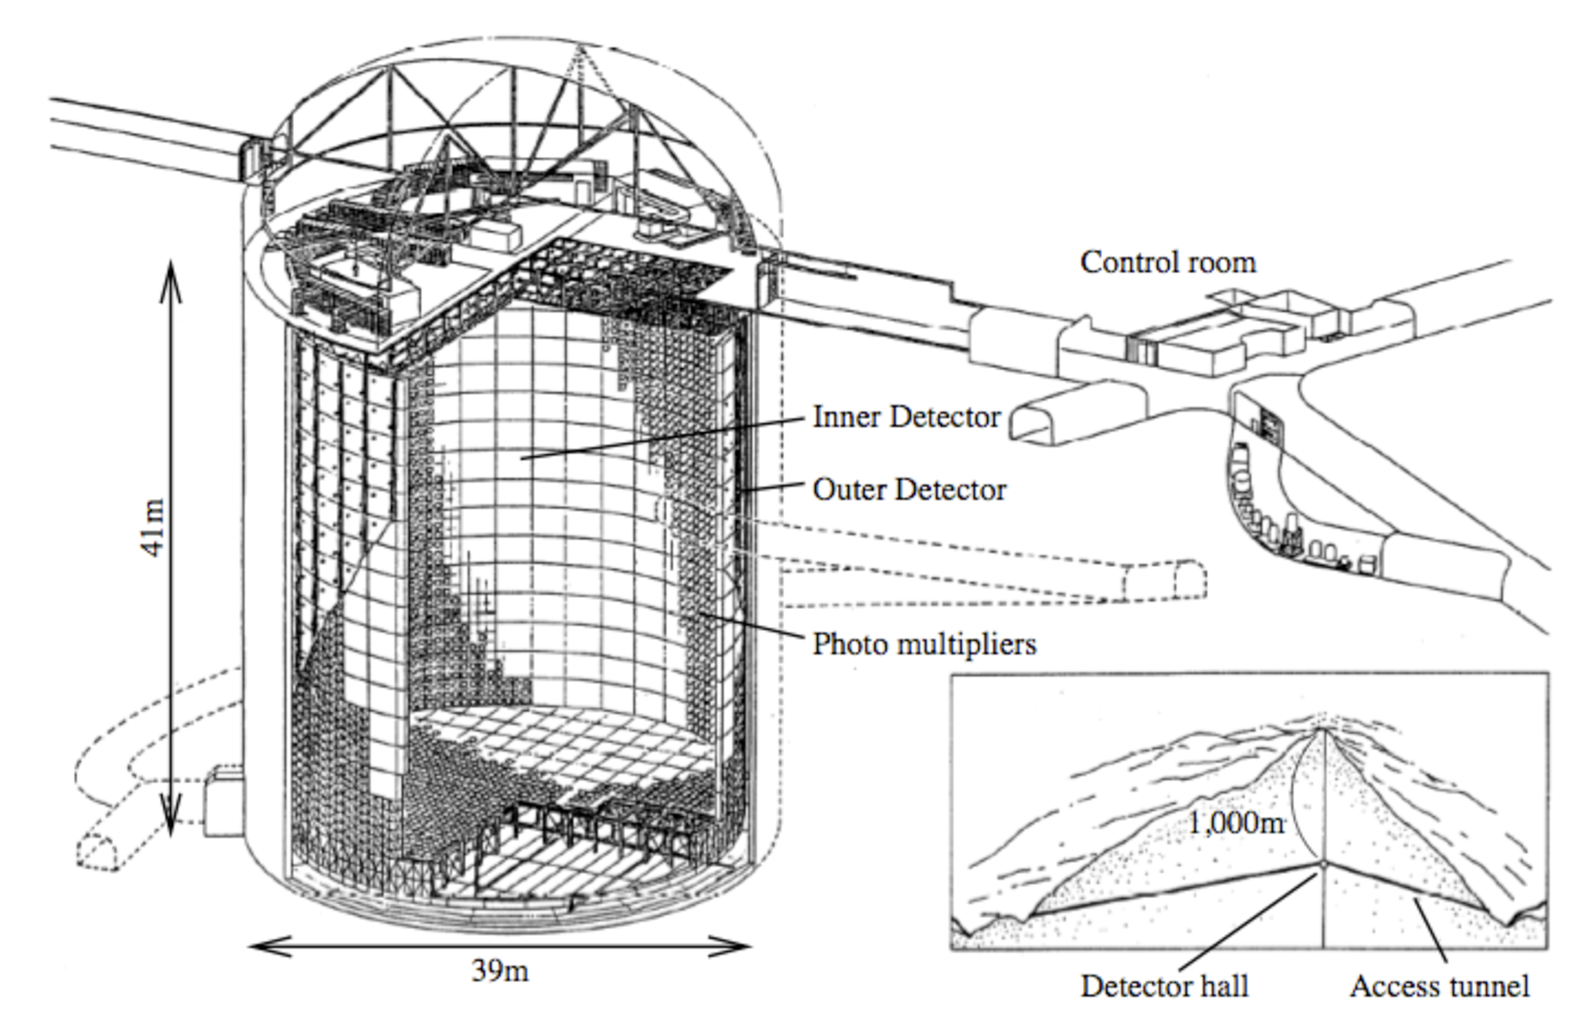
\includegraphics[width=0.8\textwidth]{images/T2K/SK_JHFDiagram.eps}
  \caption[SK detector]{Schematic view of the \Gls{SK} detector. Taken
    from~\cite{SK2003}.}
  \label{fig:sk}
\end{figure}

The inner detector is surrounded by 11,129 \Glspl{PMT} pointing
inwards of the detector, providing a 40\% photocoverage. The
\Glspl{PMT} detect the Cherenkov lights from charged particle after
neutrino interactions. There are also 1,885 \Glspl{PMT} pointing
outwards in the outer detector volume to veto events that happen
outside the detector. Each \Gls{PMT} can detect single photons. They
are sensitive to photons of wavelengths in the $350 - 500\text{~nm}$
range and the maximum quantum efficiency is reached for photons of
wavelength $\sim 400\text{~nm}$ (21~\% efficiency). The number of
photo-electrons is multiplied by a system of eleven dynodes of
Venetian blind type which are providing a gain of about $10^7$ when
operated at around $2~\text{kV}$, as is the case in
\Gls{SK}~\cite{SKPMT}.

Note that to produce Cherenkov light, a charged particle must
propagate at a velocity faster than the speed of light in the medium
it traverses. This means there is a threshold of energy for a particle
to be detected, which is given by $p>m/\sqrt{n^2-1}=m/1.27$, where $p$
and $m$ are the momentum and mass of the charged particle, and $n$ is
the refractive index of the medium, (1.3 in water).

In Figure~\ref{fig:cherenkov}, the signal produced by electrons and
muons from \Gls{TK} is shown. The somewhat simple design of the
detector allows a very efficient separation between muons and
electrons. Indeed, muons have a large mass ($105.6~\text{MeV}$) and
therefore propagate relatively straight in water. This is the reason
muons produce a clear Cherenkov ring on the \Gls{SK} wall. Electrons
on the other hand, because of their small mass, change direction and
produce \Gls{EM} showers when propagating (bremsstrahlung photons,
Compton scattering, pair production). They will produce a more poorly
defined (or ``fuzzier'') Cherenkov ring on the wall.

\begin{figure}[ht]
  \center
 % \includegraphics[width=0.8\textwidth]{images/T2K/numu_sk-eps-converted-to.pdf}\\
%  \includegraphics[width=0.8\textwidth]{images/T2K/nue_sk-eps-converted-to.pdf}
  \caption[Events observed at SK]{Events observed at
    \Gls{SK}. \textbf{\textit{Top:}} \gls{numu}
    candidate. \textbf{\textit{Bottom:}} \gls{nue} candidate. The
    Cherenkov light ring is ``fuzzier'' in the case of \gls{nue} due
    to multiple scatter of the electron. Both taken
    from~\cite{T2K2011}.}
  \label{fig:cherenkov}
\end{figure}

The detector can also detect delayed signals from Michel electrons and
detect charged current interaction with one charged pion in the final
state. In this case, if at least $30$ hits are detected
$100\text{~ns}$ after the primary trigger, a decay electron is
tagged. The electron neutrino \Gls{CC}1$\pi^\pm$ sample was introduced
for 2017 analyses~\cite{LastT2K}. It gives a higher statistical power
to the appearance signal and thus makes the \Gls{TK} experiment more
senstive to \Gls{CP} violation in the neutrion sector.






\clearpage
\newpage
\blankpage

\chapter{Electromagnetic Calorimeter data quality}
\label{chap:dataquality}


An additional task of monitoring the data quality of the
electromagnetic calorimeter was conducted during the PhD, this task is
described here. A good quality of data for the \Gls{ECal} is required
for the both analyses described in this thesis, as will be described
later. Both the analyses (Neutral Current single photon search and
\Gls{ND} electron (anti-) neutrino selection) use the \Gls{ECal} for
vetoing events and the \Gls{ND} electron (anti-) neutrino selections
uses the \Gls{ECal} for particle identification.

To ensure that the quality of the data is good for all the components
of the experiment, checks are realised by the beam, \Gls{ND} and
\Gls{SK} groups.  For the \Gls{ND}, each sub-detector is checked
individually by a data quality expert who produces monitoring plots
every week during the period of data taking and when the detector is
powered on. In the case of the \Gls{ECal}, the main quantities that
are checked are the timing, the gains, the pedestals and the event
rates, which are checked at the end of each run.

As shown in Section~\ref{subsubsec:ecal}, the \Gls{ECal} encompasses
different detectors in the \Gls{ND}. The readouts for these are all
separated into 12 Read-out Merger Modules (\Gls{RMM}) which are
collecting data from a total of 366 Trip-T Front-end Boards
(\Gls{TFB}). These \Glspl{TFB} are directly connected to each channels
(Multi-Pixel Photon counter, \Gls{MPPC}). Typically, the checks are
divided for each \Gls{RMM} and each of them is checked individually.

Once the normal operation has been established for all the
\Glspl{RMM}, a flag is uploaded to a SQL database which is later used
for processing the data. Each \Gls{RMM} is treated independently.  The
flag is a 12 bit field translated to decimal number which is assigned
between two timestamps. During the normal running of the \Gls{ECal},
the flag will be 0 (or 000 000 000 000 in the binary basis), whilst if
a \Gls{RMM} is not working normally the flag will be equal to
$2^{\text{RMM}}$. If several \Glspl{RMM} are not working properly then
the sum of these numbers will be the flag\footnote{For example, if
  \Gls{RMM}2, 3 and 11 were not working normally the bit field will
  be: 100 000 001 100, which translates to $2^{11}+2^{3}+2^{2}=2060$
  in the decimal basis.}

This task has been carried out for the 12 \Glspl{RMM} of the
\Gls{ECal} during two years. For the purpose of clarity, only the run
7 \Gls{RMM}0 data (which is the 2016 data of half of the
\Gls{DsECal}), is shown in this section, unless stated otherwise.

In the first section, the beam timing monitoring is explained; then
the monitoring of gain and pedestal are described. Finally, the
stability of event rates is demonstrated in the last section. This
section shows that the \Gls{RMM}0 of the \Gls{ECal} (and more
generally the whole \Gls{ECal}) has produced good and usable data for
run~7 data-taking period.


\section{Beam timing}
\label{sec:beamtiming}

The reconstruction good timing of the hits in the detector are
required to be able to match the track between the \Gls{ND}
sub-detectors. Knowledge of the beam timing in the \Gls{ECal} relies
on the offsets introduced by the electronics, which can be simulated.

In Figure~\ref{fig:beamtiming}, one can see some examples of timing
distributions. In this figure, one clearly sees the bunch structure of
the beam.

The blue bands are the \Gls{ECal} reset windows between each bunch. It
can happen that the high voltage fluctuates and introduces some
variations in the beam timing profile. For run 7, this has been very
rare and it is believed that all the fluctuations in these histograms
are due to changes in the configuration of the beam itself rather than
in the \Gls{ECal}. For other runs, it was noted that fluctuations
could happen if the power supply of a \Gls{RMM} changes, or if a
mistake is introduced in the cabling of the \Gls{RMM} while
maintaining the detector.

\begin{figure}[ht]
  \begin{adjustbox}{center}
    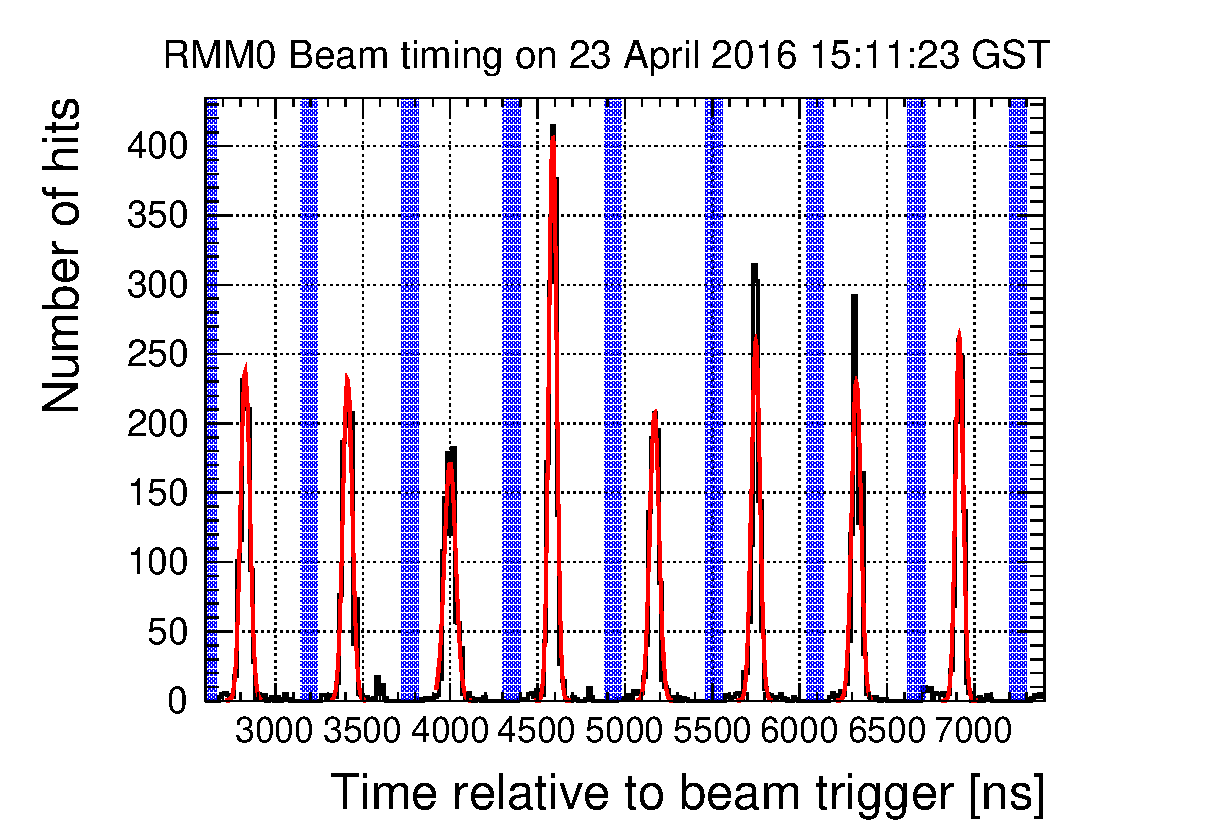
\includegraphics[width=0.48\textwidth]{images/DataQuality/BeamTimingDetail.eps}
    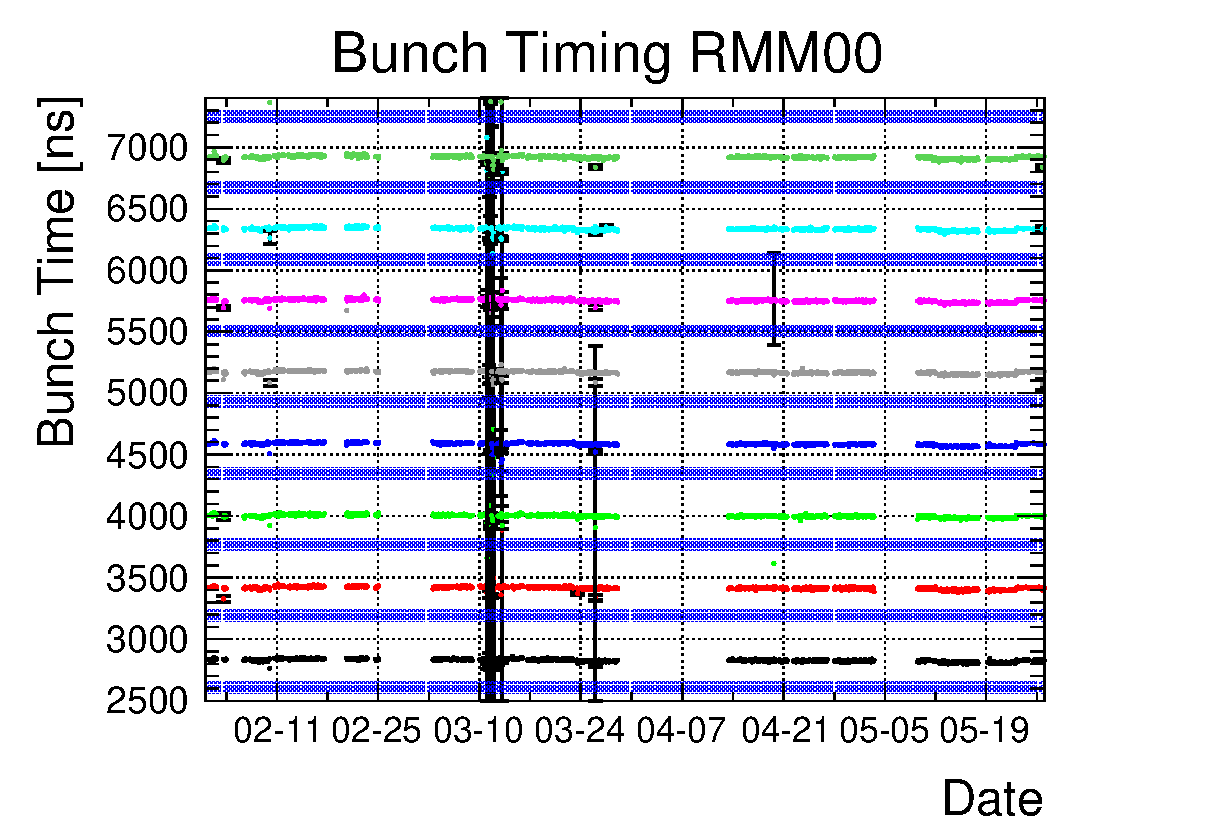
\includegraphics[width=0.48\textwidth]{images/DataQuality/BeamTimingRun7.eps} 
  \end{adjustbox}
  \caption[Run 7 beam timing data of the ECal]{\textbf{\textit{Left:}}
    Beam timing data (black) for \Gls{RMM}0 fitted by 8 Gaussian
    curves (red). \textbf{\textit{Right:}} Mean of the Gaussian fits
    over extended period for the run 7. Note that all the points with
    a large error are points for which the Gaussian fit did not
    converge properly as there were too few points to fit. The
    \Gls{ECal} reset window are in blue on both figures.}
  \label{fig:beamtiming}
\end{figure}

The check consists of producing figures such as the one on the right
of Figure~\ref{fig:beamtiming} every week, and checking that all the
points are aligned. Any deviation from constant beam timing has to be
explained and flagged accordingly.

\section{Gain and Pedestal of the MPPC}
\label{sec:gainped}

The \Gls{ECal} gains for each channel are also checked every
week. Fast and large gain variations are not desirable as they make
the calibration more complex, and can be indicative of a problem with
the \Gls{ECal} or its power supply. The \Gls{ADC}\footnote{ADC: Analog
  to Digital Converter} counts of each channel can be used to
calculate the pedestal and gain values. To do that, the \Gls{ADC}
counts are stored in a histogram over a period which corresponds to
about 20 minutes (usually 500 events). An example of the histogram is
shown in Figure~\ref{fig:DPT} for a longer period.  In this histogram,
the first peak corresponds to having no hit in the \Gls{MPPC} and is
called the pedestal. The pedestal is the \Gls{ADC} value when nothing
happens in the detector. One could manually set the pedestal value to
be read $0$ in the \Gls{ADC}, however this is not preferable because
the \Gls{ADC} is not linear in this region. The second peak
corresponds to the \Gls{ADC} output when one photo-electron fires one
pixel. The difference between the first two peaks provides a direct
measurement of the single photo-electon response, i.e. the number of
\Gls{ADC} counts for each detected photo-electron. This single
photo-electron response can be use to calculate the gain.

\begin{figure}[ht]
  \begin{adjustbox}{center}
    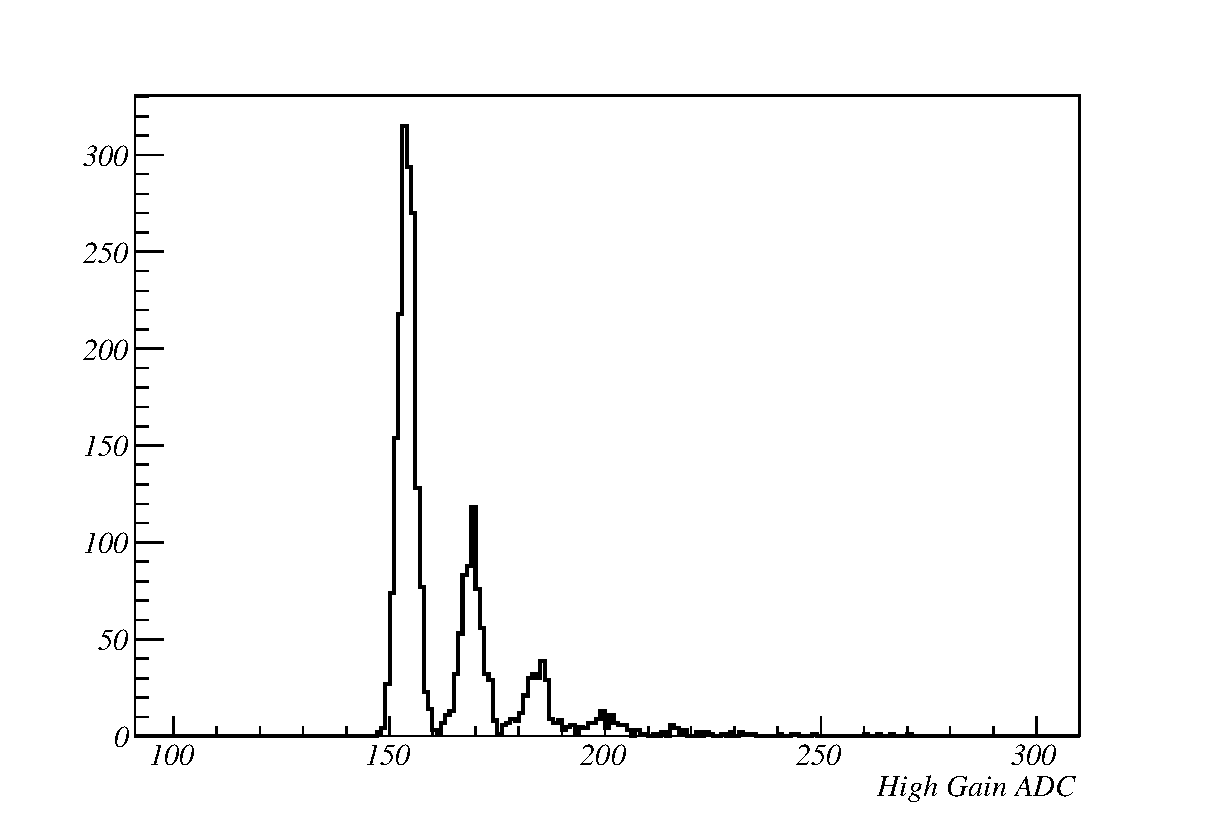
\includegraphics[width=0.8\textwidth]{images/DataQuality/highgainraw.eps}
  \end{adjustbox}
  \caption[A DPT high gain channel histogram, ECal ADC readings
  showing the first, second, third and fourth photo-electon peaks]{Few
    \Gls{ECal} \Gls{ADC} readings for the high gain channel, this
    figure is called a \Gls{DPT} (Data Processing Task) histogram. The
    histograms are realised by the processing nodes (\Gls{TFB}) by
    using the data from all the Trip-T detectors connected to the
    \Gls{TFB} during a period of around 20~min (500 events). On this
    figure, the first, second, third and fourth photo-electron peaks
    are visible from left to right. Such histograms are used during
    the calibration of the detectors. Taken from~\cite{T2KCalib}.}
  \label{fig:DPT}
\end{figure}


Every week, the value of the pedestal and gain are checked. Note that
on top of the built-in \Gls{MPPC} gain (of about $10^6$ as shown in
Subsection~\ref{subsec:mppc}), there are two electronic gain channels:
\begin{itemize}[noitemsep,topsep=0pt]
\item a high gain channel, where $1$~\Gls{PEU}\footnote{PEU: Pixel
    Equivalent Unit, is the raw value in pC of the charge detected by
    the \Gls{MPPC}.} is encoded in $\sim 10$~\Gls{ADC} counts. This
  value can be seen in the difference between the two first peaks of
  Figure~\ref{fig:DPT},
\item and a low gain channel, where a $1$~\Gls{PEU} is encoded in
  $\sim 1$~\Gls{ADC} counts.
\end{itemize}
This provides two sets of measurements relevant for many detected
photo-electrons, for the low gain channel; and few photo-electrons for
the high gain channel. For the low gain, the pedestal and the first
photo-electron peak are superimposed, and hence the equivalent of
Figure~\ref{fig:DPT} for the low gain channel would only have one
peak. This means the only gain that can be easily monitored is the
high gain. It is also the most sensitive one.

To produce the weekly plots used for the monitoring, on
Figures~\ref{fig:gain} and \ref{fig:ped}, a reference value of the
gain is taken every time calibration is done (typically once every
week). Then, the difference between the gain and the reference is
``histgrammed'' over the week for all the channels. The same procedure
is applied for the high and low pedestal. The differences should be
under 0.5 in absolute value (red line).

As for the beam timing, any deviation from the allowed regions should
be understood and flagged accordingly. Since the gain are dependant on
the temperature (see Section~\ref{subsec:mppc}), it is very common
that abrupt changes of temperature cause the gain to change to
unacceptable values. This generally happens after a long shutdown,
when the \Glspl{RMM} boards are cold, when the magnet is being closed
or when the magnetic field is turned off of on. Additionally, extreme
weather variations can cause unwanted gain variations. ``Turn-on''
effects are visible on Figures~\ref{fig:gain} and \ref{fig:ped}, where
the gain and pedestal value change abruptly in the beginning of the
run or after the winter shutdown.

\begin{figure}[ht]
  \begin{adjustbox}{center}
    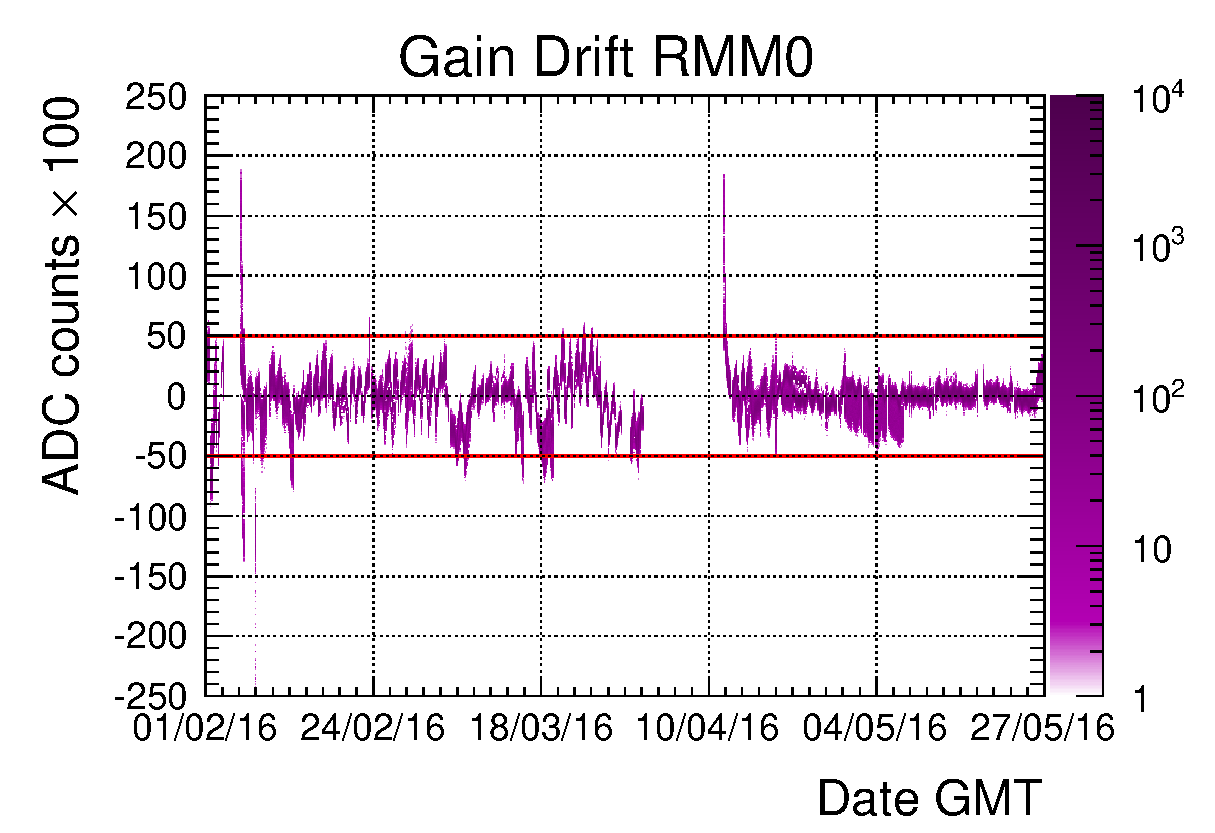
\includegraphics[width=0.58\textwidth]{images/DataQuality/gaindrift.eps}
  \end{adjustbox}
  \caption[Run 7 ECal RMM0 gain drifts]{\Gls{ECal} \Gls{RMM}0 gain
    drifts over run 7.}
  \label{fig:gain}
\end{figure}


\begin{figure}[ht]
  \begin{adjustbox}{center}
    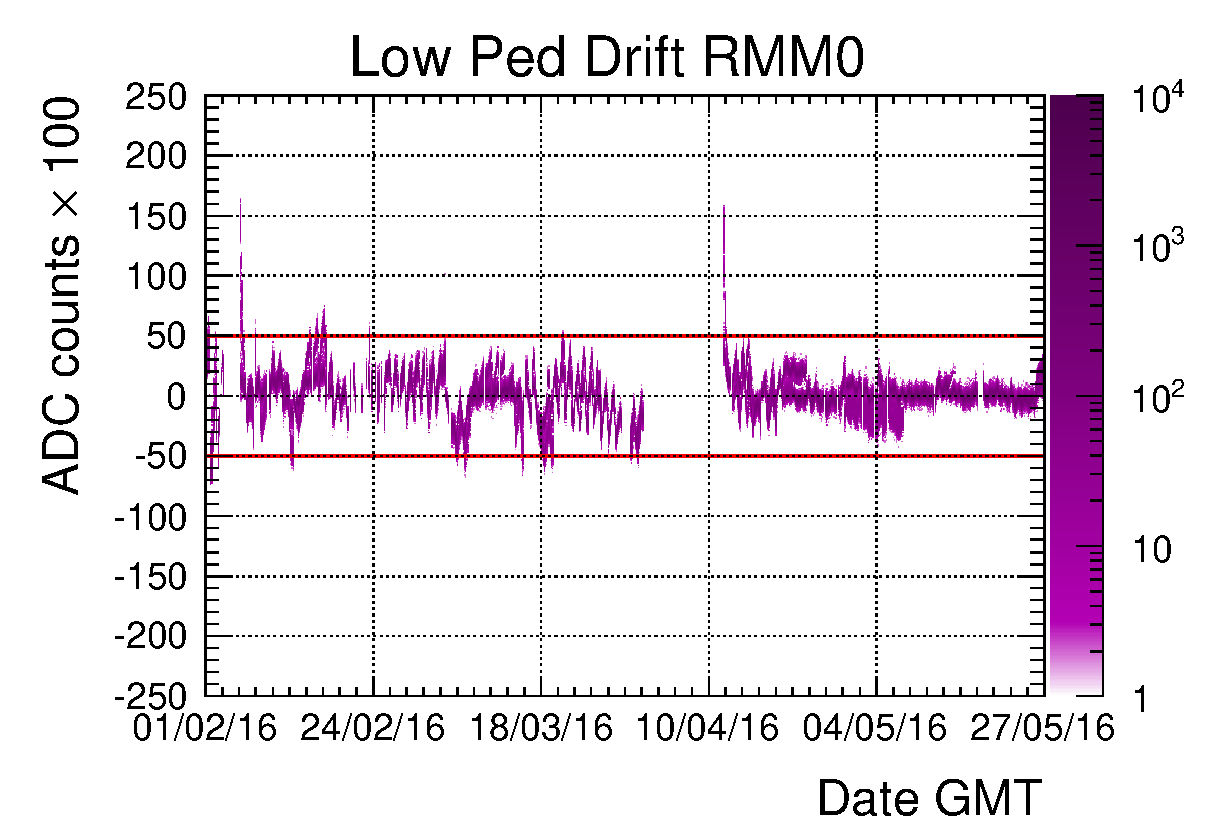
\includegraphics[width=0.48\textwidth]{images/DataQuality/lowped.eps} 
    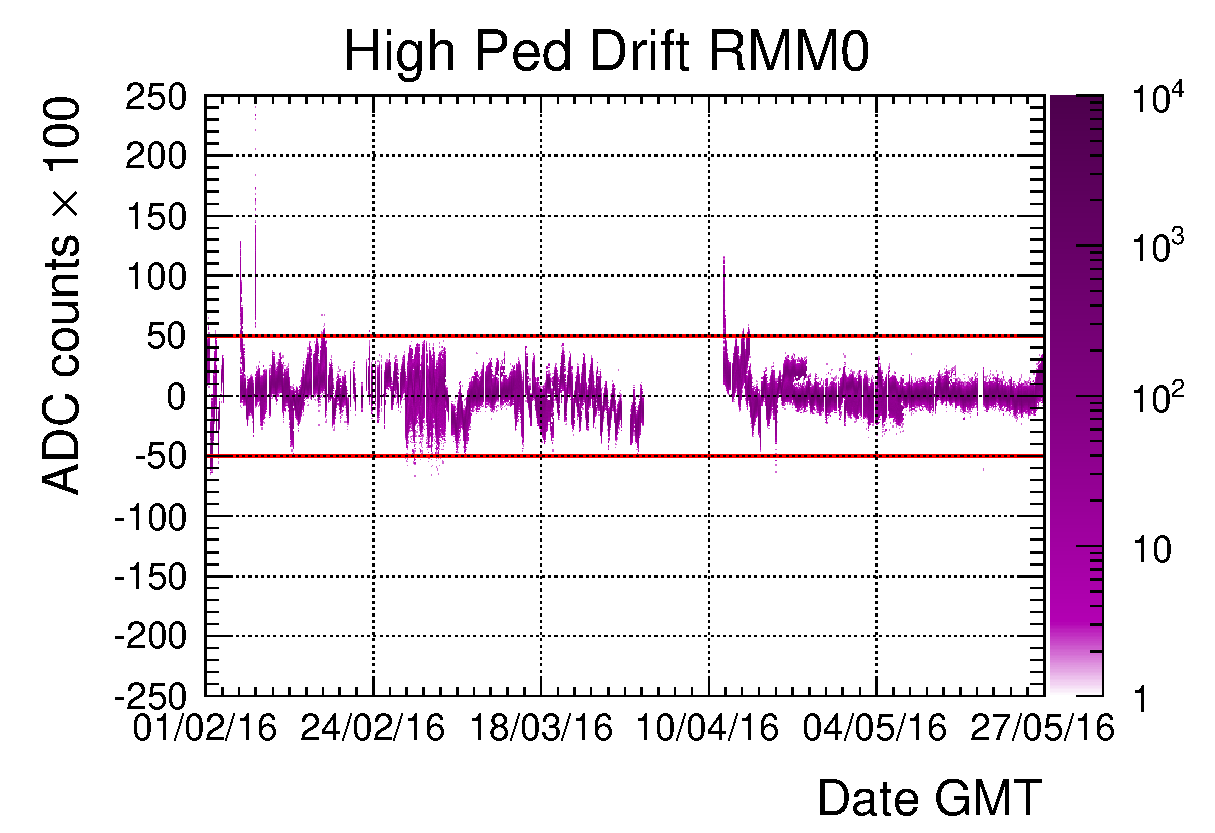
\includegraphics[width=0.48\textwidth]{images/DataQuality/highped.eps}
  \end{adjustbox}
  \caption[Run 7 ECal pedestal drifts]{\Gls{ECal} \Gls{RMM}0 pedestal
    drifts over run 7. \textbf{\textit{Left:}} Low
    pedestal. \textbf{\textit{Right:}} High pedestal.}
  \label{fig:ped}
\end{figure}

\section{Event rates}
\label{sec:eventrate}
Another final check that is realised consists in checking the event
rate of the \Gls{ECal}.  This is done once at the end of the run. To
do this, a simple cluster algorithm is run on the data. One can then
normalise the number of reconstructed clusters by the number of
\Gls{POT} (Protons on Target). If the \Gls{ECal} runs normally, this
number should be constant over time. Some changes can happen if the
horn current is modified (if the horn current increases, for example,
more neutrinos are going to be focused and reach the \Gls{ECal} thus
increasing the event rate). Similarly, if the horn polarity is
reversed, the fraction of neutrinos and anti-neutrinos reaching the
\Gls{ECal} will be different and will lead to different event
rates.

The result for run 7 is shown in Figure~\ref{fig:eventrate} (in this
figure, all the \Glspl{RMM} cluster\footnote{A cluster is defined here
  as at least three hits (i.e. at least one detected photo-electron
  for three different bars), in adjancent bars, in a time window of
  $30\text{~ns}$. The cluster is expanded from the highest detected
  charge to neighboring bars. Note that for physics purpose, the
  number of required hits is seven, which is an additional security to
  noise clusters.} rates are summed). One can see that the event rate
for anti-neutrino mode is smaller than in neutrino mode. This happens
because the both the anti-neutrino flux and cross section are much
smaller than the in the neutrino case. As can be seen, some problems
happened around mid-April, when the part of the \Gls{BrECal} was
turned off due to a cooling issue.

\begin{figure}[ht]
  \begin{adjustbox}{center}
    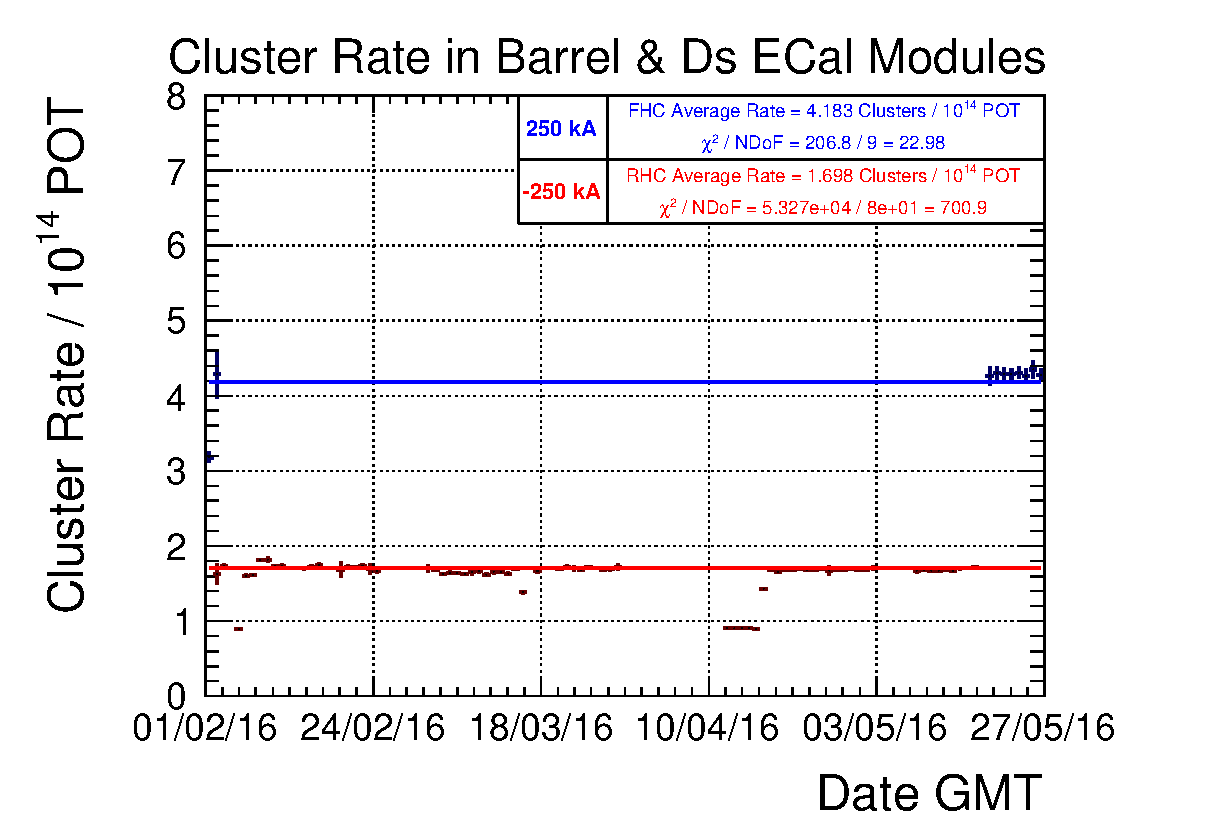
\includegraphics[width=0.7\textwidth]{images/DataQuality/ClusterRates.eps} 
  \end{adjustbox}
  \caption[Run 7 ECal cluster rate]{Cluster rate for all the
    \Gls{ECal} during run 7, during which the horn polarity was
    positive (\Gls{FHC}, in blue) and negative (\Gls{RHC}, in red).}
  \label{fig:eventrate}
\end{figure}


\section{Summary}
\label{sec:dqsummary}
From the three sections developed in this chapter, it is clear that
the \Gls{ECal} of the \Gls{ND} delivers good and usable
data. Monitoring the data quality is a fundamental step during the
data-taking periods which ensures fast feedback and diagnostic of the
problem to the expert in charge of the maintenance of the
detector. This is critical as the \Gls{TK} collaboration has to make
sure that all the allocated beam time of the experiment can be used
for physics analysis and thus address any hardware issue as fast as
possible. The \Gls{ECal} data has found many use for \Gls{ND} analyses
(high angles~\cite{TN310,TN348}, \Gls{ECal} as target
analyses~\cite{DomBrailsford2016}) which includes the two analyses
described in this thesis (\Gls{NCg} and electron (anti-) neutrino
selections).





\clearpage

\chapter{Neutrino Neutral Current single photon phenomenology}
\label{chap:pheno}

This section covers the description of the ``\Gls{NC} gamma'', or
single photon neutrino-production processes in more details. There is
no data that can constrain the cross section calculations that have
been made up to now, however some models are more theoretically
motivated than others. There are two main reasons why the \Gls{NCg}
interactions have an importance in the accelerator neutrino physics:
\begin{itemize}[noitemsep,topsep=0pt]
\item The background in the so-called \Gls{MiniBooNE} low-energy
  excess~\cite{MBexcess2009,AnuMiniBooNE2013}: This excess was
  discovered in the electron (anti-) neutrino samples of the
  \Gls{MiniBooNE} Cherenkov detector. \Gls{NCg} processes are one of
  the background for the electron (anti-) neutrino samples. The
  presence of these processes with cross section enhanced by a factor
  of 2.7 could explain this excess~\cite{MBexcess2009}.
\item The background for search for \Gls{CP} violation at \Gls{TK} or
  \Gls{NOvA}: Similarly to the \Gls{MiniBooNE} analyses, \Gls{NCg}
  events are one of the background for electron (anti-)
  neutrinos. From the last \Gls{TK} result~\cite{LastT2K}, it is clear
  that this background is already a problem.
\end{itemize}

The reason \Gls{NCg} events systematically are present in the electron
(anti-) neutrino samples was developed earlier, it is because the
photons and electrons produce the same signal in Cherenkov detectors
(see Section~\ref{subsubsec:ncgprocesses}).

Firstly, the models leading to these events are described, then the
generator implementation of the models are explained. Accurate
modeling of the \Gls{NCg} processes becomes increasingly important as
statistics in the electron sample increase and therefore the
statistical uncertainty on these becomes smaller. All the available
predictions (from generators and different theories) are summarised in
Figure~\ref{fig:integratedncg} for the integrated cross sections and
Figure~\ref{fig:diffncg} for simple one-dimensional differential cross
sections.

\begin{figure}[ht]
  \center
  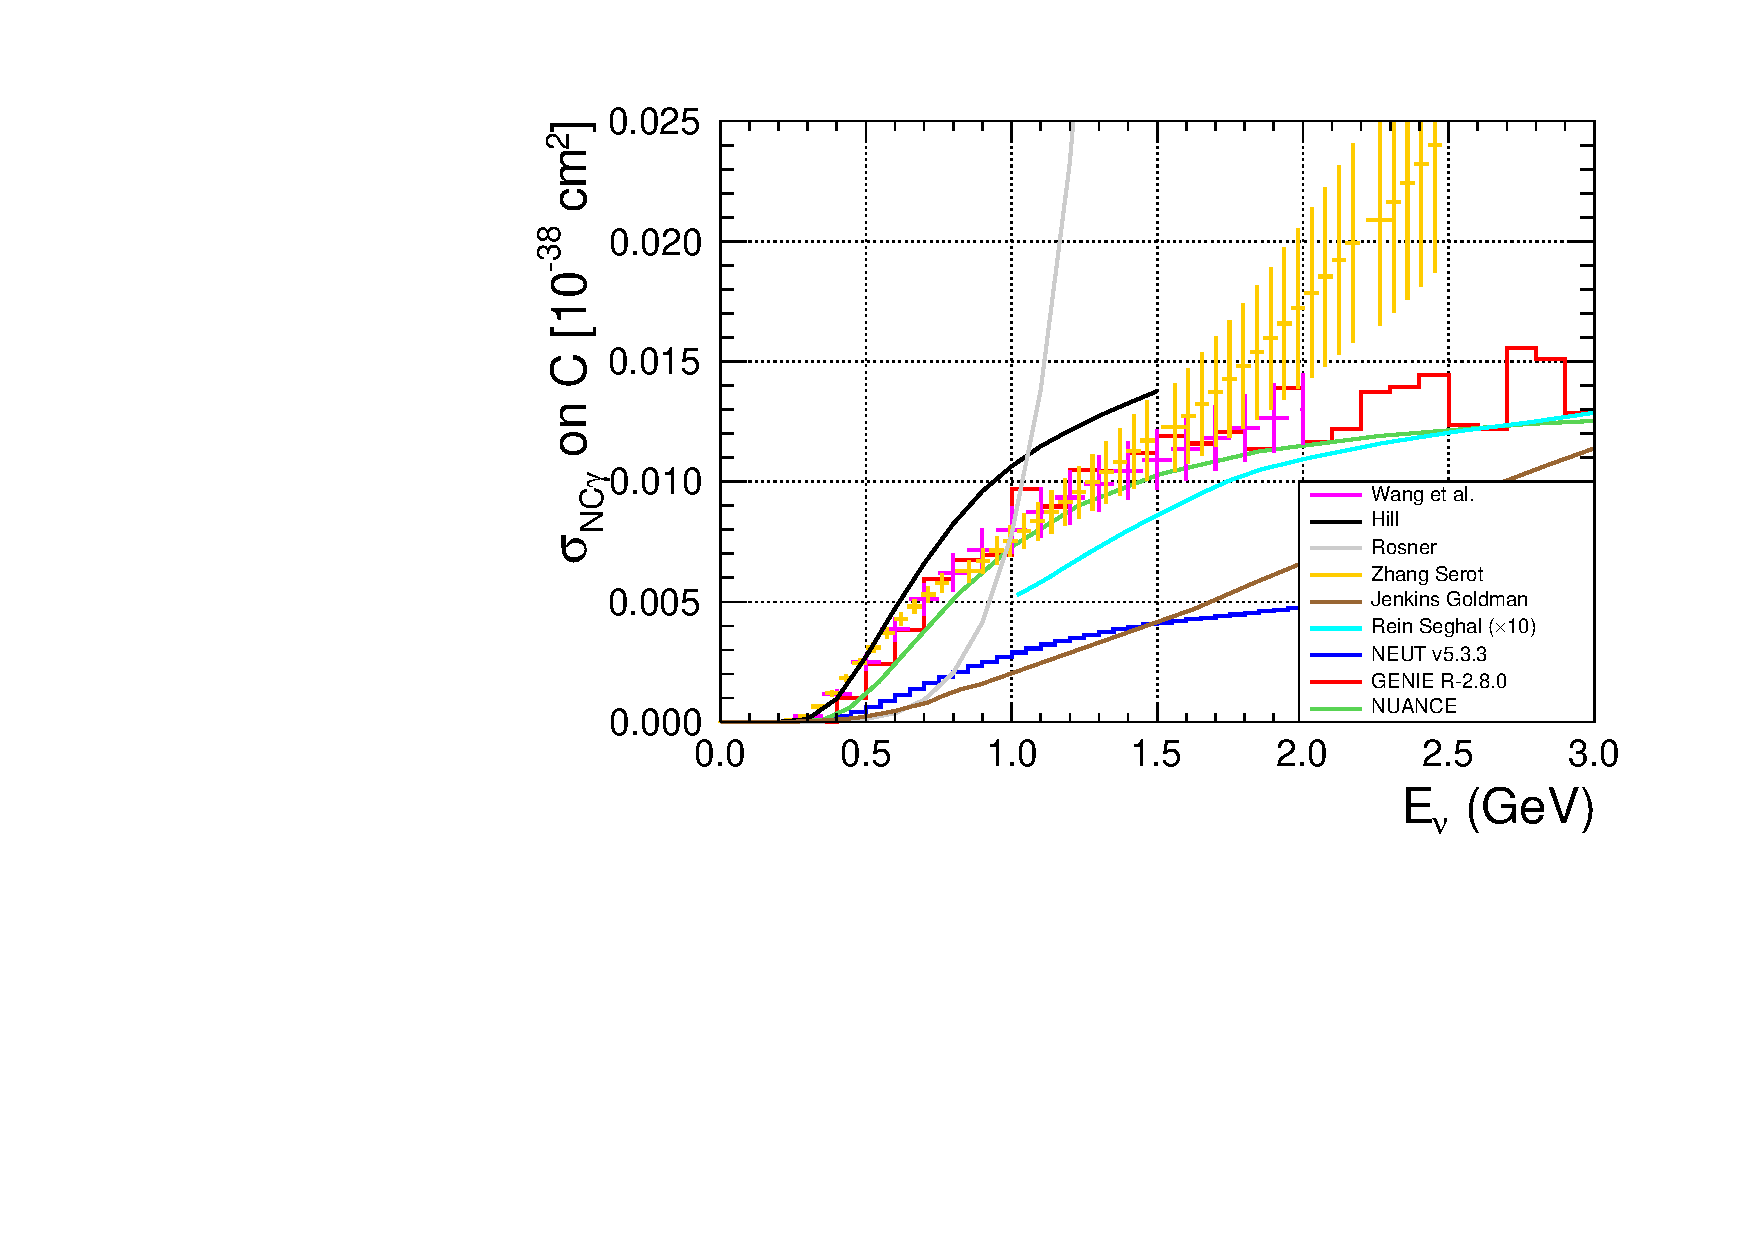
\includegraphics[width=0.68\textwidth]{images/Pheno/NCG_integrated.pdf}
  \caption[Integrated cross section for neutrino single photon
  production on carbon]{Integrated cross section for neutrino single
    photon production on carbon, based on the theoretical work from:
    Wang~et~al.~\cite{Alvarez2014}, Hill~\cite{Hills2007},
    Rosner~\cite{Rosner2015}, Zhang~et~al.~\cite{Serot2012}, Jenkins
    Goldman~\cite{Jenkins}, Rein Seghal~\cite{ReinCohGamma}. The
    following are neutrino interaction generators:
    \Gls{NEUT}~\cite{NEUT}, \Gls{GENIE}~\cite{GENIE1,GENIE2} and
    \Gls{NUANCE}~\cite{nuance}. Figure based on~\cite{Garvey:2014exa}
    (Figure~43).}
  \label{fig:integratedncg}
\end{figure}

\begin{figure}[ht]
  \center
  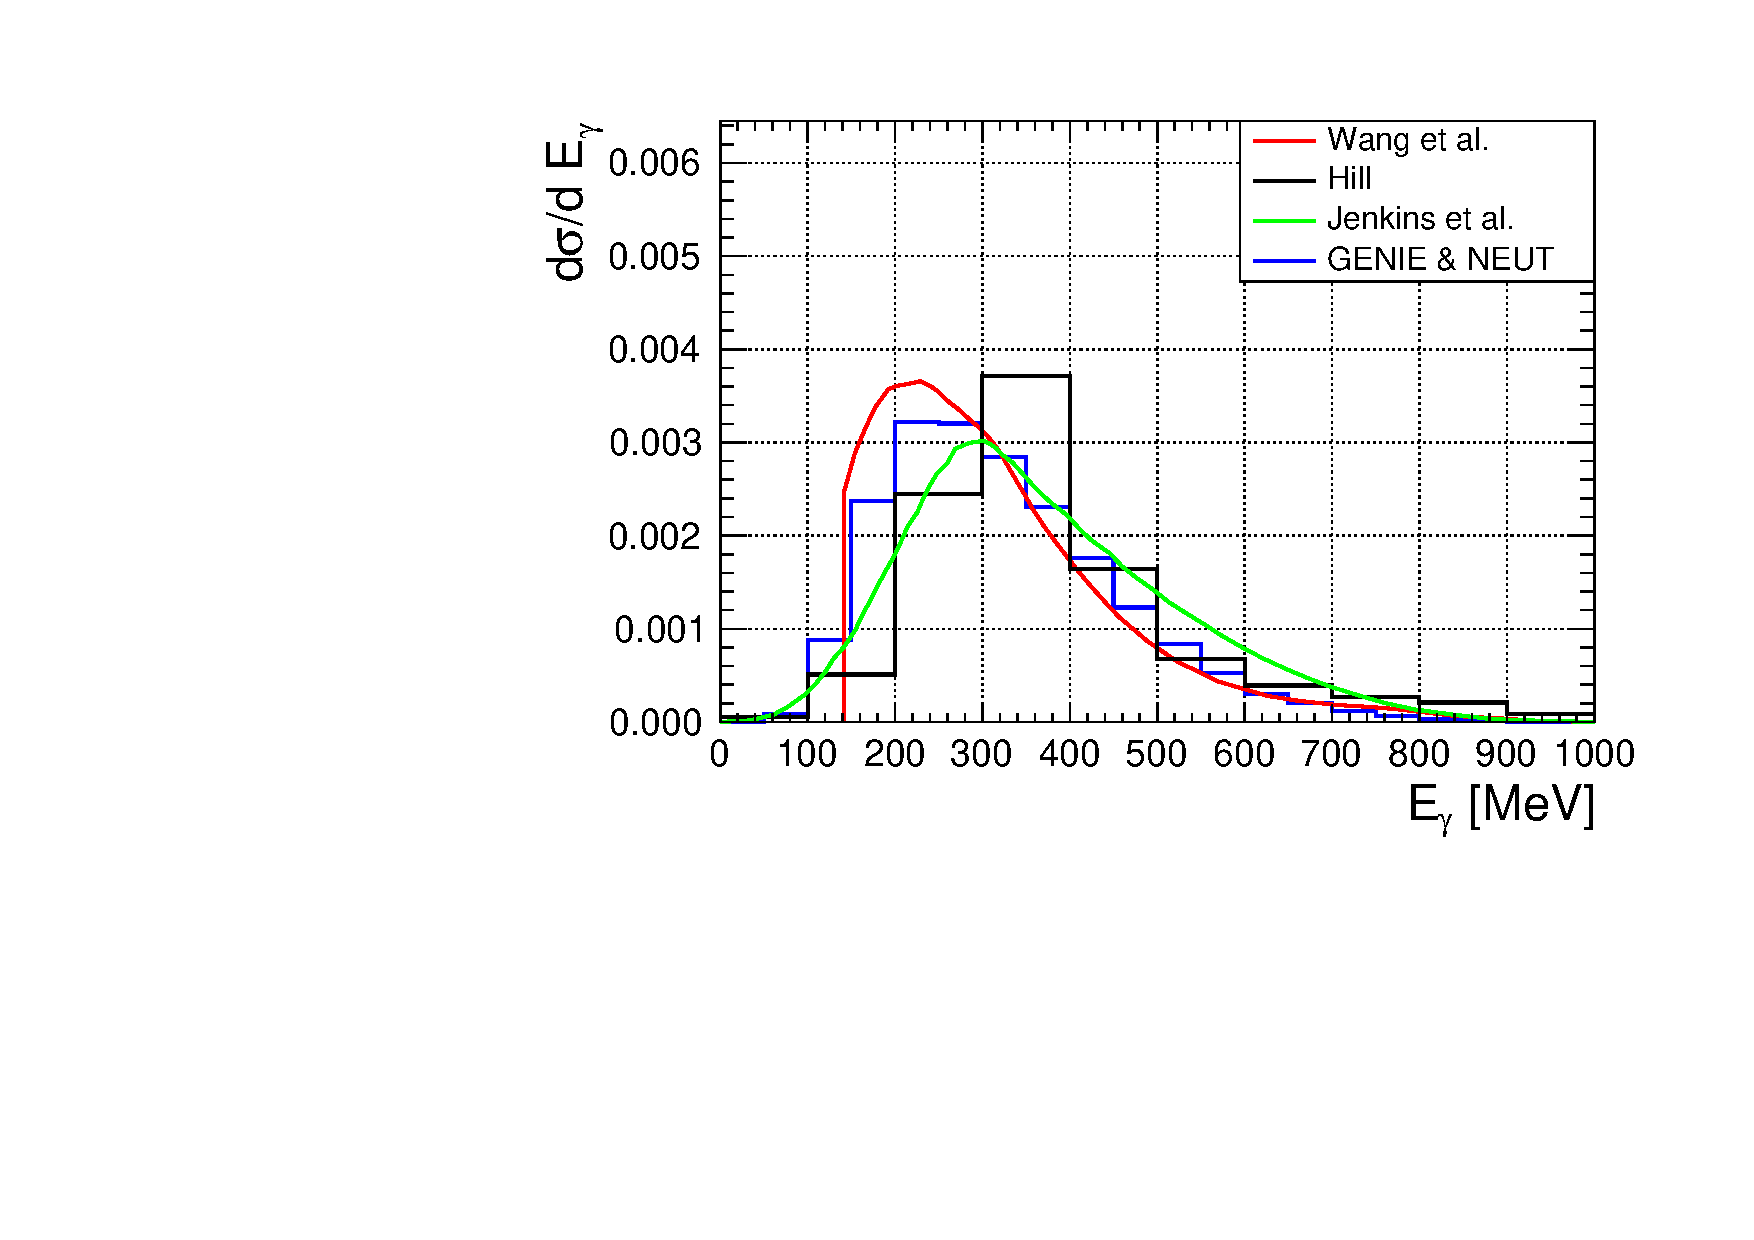
\includegraphics[width=0.7\textwidth]{images/Pheno/NCG_Diff_ene.pdf}
  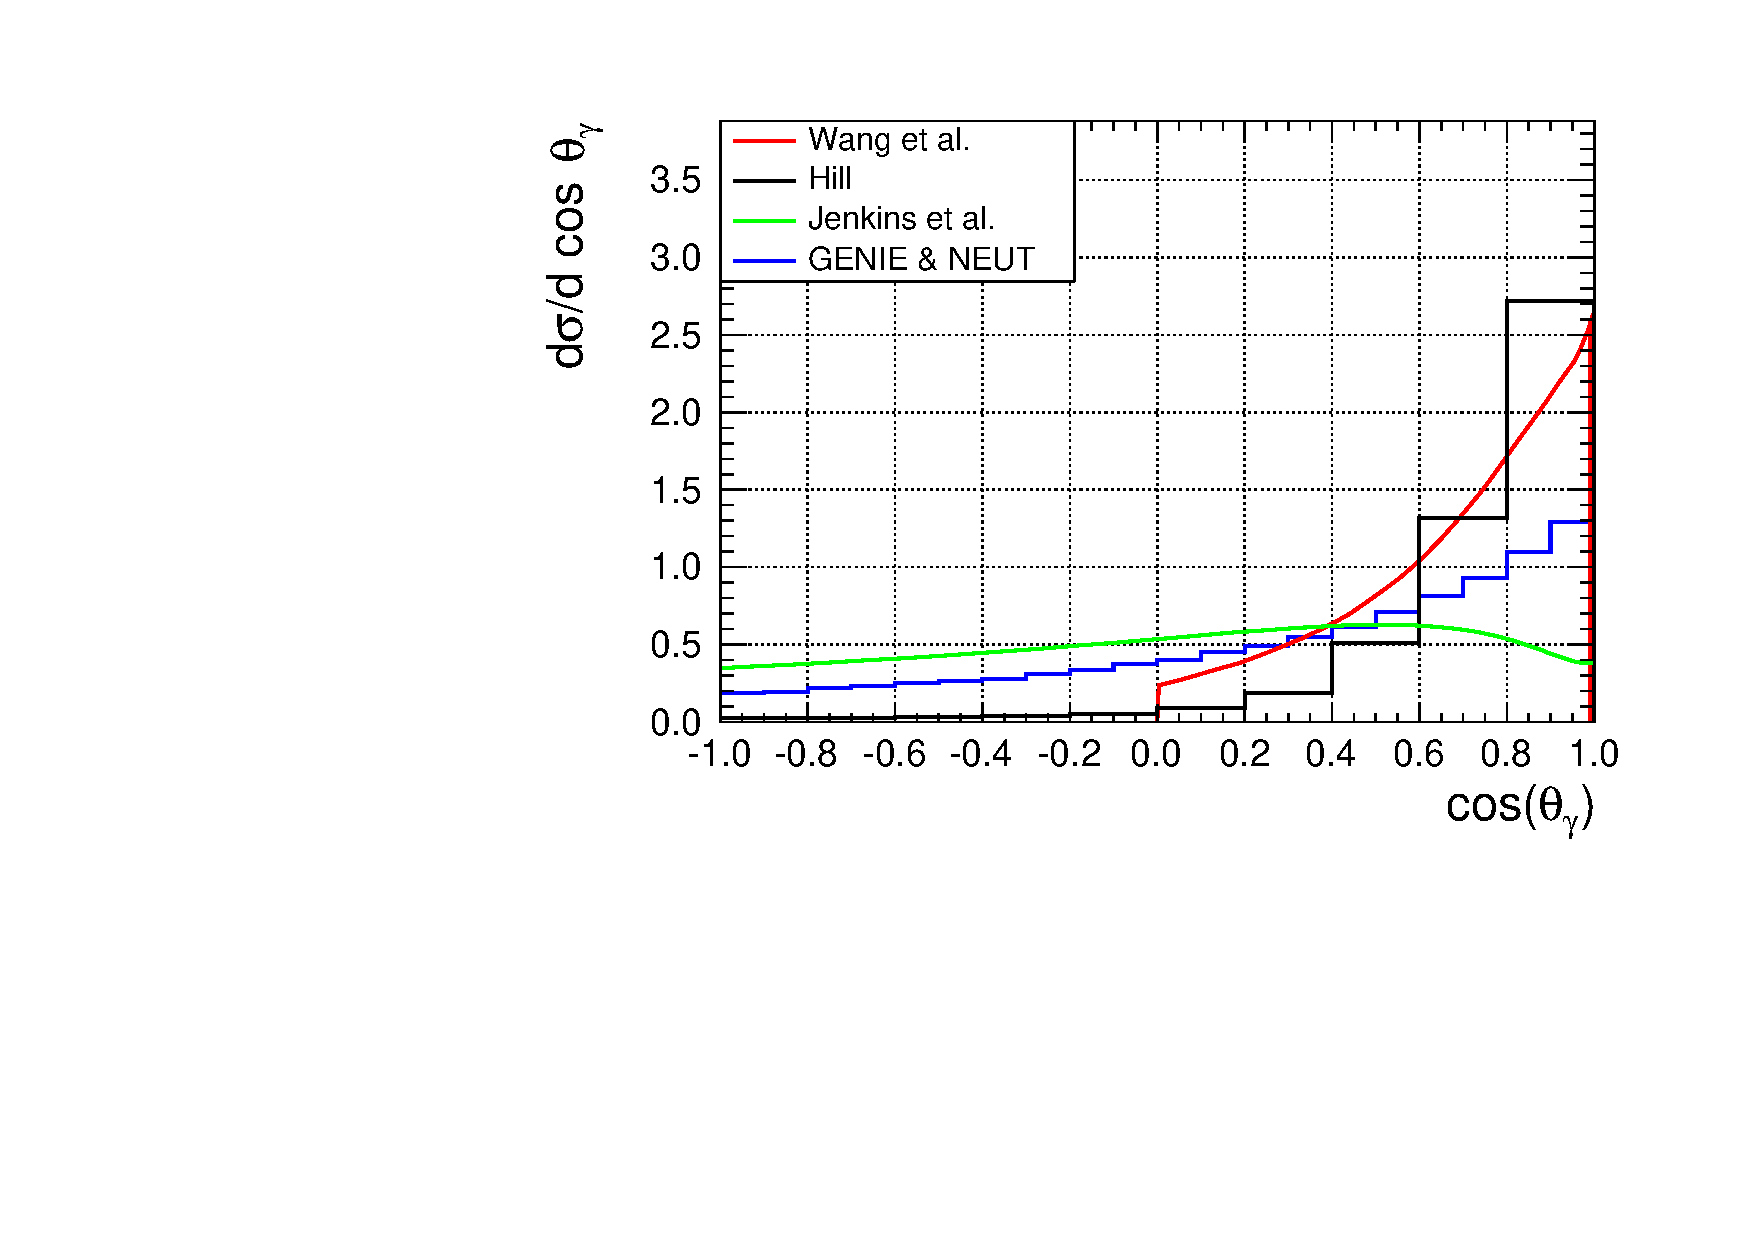
\includegraphics[width=0.7\textwidth]{images/Pheno/NCG_Diff_cos.pdf}
  \caption[Differential cross sections for a 1~GeV neutrino single
  photon production on carbon]{Differential cross sections for a
    $1$~GeV neutrino single photon production on
    carbon. \textbf{\textit{Top:}} Differential cross section in
    photon energy. \textbf{\textit{Bottom:}} Differential cross
    section in photon angle (right), based on the theoretical work
    from: Wang~et~al.~\cite{Alvarez2014}, Hill~\cite{Hills2007},
    Jenkins Goldman~\cite{Jenkins}, \Gls{NEUT}~\cite{NEUT}. The
    following are neutrino interaction generators:
    \Gls{GENIE}~\cite{GENIE1,GENIE2}. All the distributions have been
    normalised to unit area. The \Gls{NEUT} and \Gls{GENIE}
    distributions are almost identical, so only the \Gls{NEUT}
    distribution was kept for clarity.}
  \label{fig:diffncg}
\end{figure}
\clearpage

\section{Models}
\label{sec:models}

Figure~\ref{fig:FeynmanDiagramNCG} shows the Feynman diagrams that are
used in recent
calculations~\cite{Alvarez2014,Hills2007,Rosner2015,Serot2012,Jenkins,ReinCohGamma}. All
the models use a resonant production model based on the chiral
description of the nucleus, except the Rein and Sehgal model which
only has the coherent contribution. Note that this is a different
model to the one that is implemented in the generators.

The model in~\cite{Alvarez2014} carefully estimates the
background~/~$\Delta$~/~higher resonances interferences by adding
coherently all the amplitudes of the Feynman diagrams in
Figure~\ref{fig:FeynmanDiagramNCG} (contribution 1 to 6). The model in
\cite{Hills2007} takes into account a the $\Delta$ contribution (1 in
the figure), and an additional anomalous countribution (9 in the
figure) All the known effects due to the nuclear medium are also taken
into account.  Figure~\ref{fig:diffncg} shows the differential one
dimensional cross section available for the \Gls{NCg}.

\begin{figure}[ht]
  \center
  \textbf{\textit{1)}}\hspace{1cm}\begin{fmffile}{feynmandiag/directdelta}
    \begin{fmfgraph*}(27,27)
      \fmfstraight
      \fmftop{i2,o3}
      \fmfleft{i1,b2,b3,i2}
      \fmfright{o1,o2,o3}
      \fmfbottom{i1,o1}
      \fmf{fermion,tension=1.5}{i2,v1}
      \fmflabel{$\nu$}{i2}
      \fmf{fermion}{v1,o3}
      \fmflabel{$\nu$}{o3}
      \fmf{fermion,tension=1.7}{i1,v2}
      \fmflabel{$n/p$}{i1}
      % \fmfstraight
      \fmf{dbl_plain_arrow,label=$\Delta$,tension=2}{v2,v3}
      \fmf{photon,label=$Z^0$}{v1,v2}
      \fmf{photon,tension=1.5}{v3,o2}
      \fmflabel{$\gamma$}{o2}
      \fmf{fermion}{v3,o1}
      \fmflabel{$n/p$}{o1}
    \end{fmfgraph*}
  \end{fmffile} 
  \hspace{2cm}
  \textbf{\textit{2)}}\hspace{1cm}\begin{fmffile}{feynmandiag/indirectdelta}
    \begin{fmfgraph*}(27,27)
      \fmfstraight
      \fmftop{i2,o4}
      \fmfleft{i1,b2,b3,i2}
      \fmfright{o1,o2,o3,o4}
      \fmfbottom{i1,o1}
      \fmf{fermion,tension=2}{i2,v1}
      \fmflabel{$\nu$}{i2}
      \fmf{fermion}{v1,o4}
      \fmflabel{$\nu$}{o4}
      \fmf{fermion,tension=3}{i1,v2}
      \fmflabel{$n/p$}{i1}
      % \fmfstraight
      \fmf{dbl_plain_arrow,label=$\Delta$}{v2,v3}
      \fmf{photon}{v1,v3}
      % \fmflabel{$Z^0$}{v1}
      \fmf{photon,tension=1.4}{v2,o3}
      \fmflabel{$\gamma$}{o3}
      \fmf{fermion,tension=3}{v3,o1}
      \fmflabel{$n/p$}{o1}
      \fmffreeze
      \fmf{phantom,label.dist=0,label=$Z^0$}{v1,o3}
    \end{fmfgraph*}
  \end{fmffile}

  \vspace{1cm}
  \textbf{\textit{3)}}\hspace{1cm}\begin{fmffile}{feynmandiag/directother}
    \begin{fmfgraph*}(27,27)
      \fmfstraight
      \fmftop{i2,o3}
      \fmfleft{i1,b2,b3,i2}
      \fmfright{o1,o2,o3}
      \fmfbottom{i1,o1}
      \fmf{fermion,tension=1.5}{i2,v1}
      \fmflabel{$\nu$}{i2}
      \fmf{fermion}{v1,o3}
      \fmflabel{$\nu$}{o3}
      \fmf{fermion,tension=1.7}{i1,v2}
      \fmflabel{$n/p$}{i1}
      % \fmfstraight
      \fmf{dbl_plain_arrow,label=$N^*$,tension=2}{v2,v3}
      \fmf{photon,label=$Z^0$}{v1,v2}
      \fmf{photon,tension=1.5}{v3,o2}
      \fmflabel{$\gamma$}{o2}
      \fmf{fermion}{v3,o1}
      \fmflabel{$n/p$}{o1}
    \end{fmfgraph*}
  \end{fmffile}
  \hspace{2cm} 
  \textbf{\textit{4)}}\hspace{1cm}\begin{fmffile}{feynmandiag/indirectother}
    \begin{fmfgraph*}(27,27)
      \fmfstraight
      \fmftop{i2,o4}
      \fmfleft{i1,b2,b3,i2}
      \fmfright{o1,o2,o3,o4}
      \fmfbottom{i1,o1}
      \fmf{fermion,tension=2}{i2,v1}
      \fmflabel{$\nu$}{i2}
      \fmf{fermion}{v1,o4}
      \fmflabel{$\nu$}{o4}
      \fmf{fermion,tension=3}{i1,v2}
      \fmflabel{$n/p$}{i1}
      % \fmfstraight
      \fmf{dbl_plain_arrow,label=$N^*$}{v2,v3}
      \fmf{photon}{v1,v3}
      % \fmflabel{$Z^0$}{v1}
      \fmf{photon,tension=1.4}{v2,o3}
      \fmflabel{$\gamma$}{o3}
      \fmf{fermion,tension=3}{v3,o1}
      \fmflabel{$n/p$}{o1}
      \fmffreeze
      \fmf{phantom,label.dist=0,label=$Z^0$}{v1,o3}
    \end{fmfgraph*}
  \end{fmffile}

  \vspace{1cm}
  \textbf{\textit{5)}}\hspace{1cm}\begin{fmffile}{feynmandiag/directnucleon}
    \begin{fmfgraph*}(27,27)
      \fmfstraight
      \fmftop{i2,o3}
      \fmfleft{i1,b2,b3,i2}
      \fmfright{o1,o2,o3}
      \fmfbottom{i1,o1}
      \fmf{fermion,tension=1.5}{i2,v1}
      \fmflabel{$\nu$}{i2}
      \fmf{fermion}{v1,o3}
      \fmflabel{$\nu$}{o3}
      \fmf{fermion,tension=1.7}{i1,v2}
      \fmflabel{$n/p$}{i1}
      % \fmfstraight
      \fmf{fermion,label=$n/p$,tension=2}{v2,v3}
      \fmf{photon,label=$Z^0$}{v1,v2}
      \fmf{photon,tension=1.5}{v3,o2}
      \fmflabel{$\gamma$}{o2}
      \fmf{fermion}{v3,o1}
      \fmflabel{$n/p$}{o1}
    \end{fmfgraph*}
  \end{fmffile}
  \hspace{2cm} 
  \textbf{\textit{6)}}\hspace{1cm}\begin{fmffile}{feynmandiag/indirectnucleon}
    \begin{fmfgraph*}(27,27)
      \fmfstraight
      \fmftop{i2,o4}
      \fmfleft{i1,b2,b3,i2}
      \fmfright{o1,o2,o3,o4}
      \fmfbottom{i1,o1}
      \fmf{fermion,tension=2}{i2,v1}
      \fmflabel{$\nu$}{i2}
      \fmf{fermion}{v1,o4}
      \fmflabel{$\nu$}{o4}
      \fmf{fermion,tension=3}{i1,v2}
      \fmflabel{$n/p$}{i1}
      % \fmfstraight
      \fmf{fermion,label=$n/p$}{v2,v3}
      \fmf{photon}{v1,v3}
      % \fmflabel{$Z^0$}{v1}
      \fmf{photon,tension=1.4}{v2,o3}
      \fmflabel{$\gamma$}{o3}
      \fmf{fermion,tension=3}{v3,o1}
      \fmflabel{$n/p$}{o1}
      \fmffreeze
      \fmf{phantom,label.dist=0,label=$Z^0$}{v1,o3}
    \end{fmfgraph*}
  \end{fmffile}

  \vspace{1cm}
  \textbf{\textit{7)}}\hspace{1cm}\begin{fmffile}{feynmandiag/pionex}
    \begin{fmfgraph*}(27,27)
      \fmfstraight
      \fmftop{i2,o4}
      \fmfleft{i1,b2,b3,i2}
      \fmfright{o1,o2,o3}
      \fmfbottom{i1,o1}
      \fmf{fermion}{i2,v1}
      \fmflabel{$\nu$}{i2}
      \fmf{fermion}{v1,o4}
      \fmflabel{$\nu$}{o3}
      \fmf{fermion}{i1,v3}
      \fmflabel{$n/p$}{i1}
      % \fmfstraight
      \fmf{photon,label=$Z^0$}{v1,v2}
      \fmf{dashes,label=$\pi^0/\omega^0/\rho^0$}{v2,v3}
      % \fmflabel{$Z^0$}{v1}
      \fmf{photon}{v2,o2}
      \fmflabel{$\gamma$}{o2}
      \fmf{fermion}{v3,o1}
      \fmflabel{$n/p$}{o1}
    \end{fmfgraph*}
  \end{fmffile}
  \hspace{2cm} 
  \textbf{\textit{8)}}\hspace{1cm}\begin{fmffile}{feynmandiag/contact}
    \begin{fmfgraph*}(27,27)
      \fmfstraight
      \fmftop{i2,o4}
      \fmfleft{i1,b2,b3,i2}
      \fmfright{o1,o2,o3}
      \fmfbottom{i1,o1}
      \fmf{fermion}{i2,v1}
      \fmflabel{$\nu$}{i2}
      \fmf{fermion}{v1,o4}
      \fmflabel{$\nu$}{o3}
      \fmf{fermion,tension=1.5}{i1,v2}
      \fmflabel{$n/p$}{i1}
      % \fmfstraight
      \fmf{photon,label=$Z^0$}{v1,v2}
      % \fmflabel{$Z^0$}{v1}
      \fmf{photon}{v2,o2}
      \fmflabel{$\gamma$}{o2}
      \fmf{fermion}{v2,o1}
      \fmflabel{$n/p$}{o1}
    \end{fmfgraph*}
  \end{fmffile}

  \vspace{1cm}
  \textbf{\textit{9)}}\hspace{1cm}\begin{fmffile}{feynmandiag/anomaly}
    \begin{fmfgraph*}(27,27)
      \fmfstraight
      \fmftop{i2,o4}
      \fmfleft{i1,b2,b3,i2}
      \fmfright{o1,o2,o3}
      \fmfbottom{i1,o1}
      \fmf{fermion}{i2,v1}
      \fmflabel{$\nu$}{i2}
      \fmf{fermion}{v1,o4}
      \fmflabel{$\nu$}{o3}
      \fmf{fermion}{i1,v3}
      \fmflabel{$n/p$}{i1}
      % \fmfstraight
      \fmf{photon,label=$Z^0$}{v1,v4}
      \fmf{dashes,label=$\omega^0$}{v5,v3}
      % \fmflabel{$Z^0$}{v1}
      \fmf{photon}{v6,o2}
      \fmf{fermion,tension=0.5}{v4,v5,v6,v4}
      \fmflabel{$\gamma$}{o2}
      \fmf{fermion}{v3,o1}
      \fmflabel{$n/p$}{o1}
    \end{fmfgraph*}
  \end{fmffile}
  
  \caption[Feynman diagrams contributing to the neutrino production of
    a single photon]{Feynman diagrams contributing to the neutrino production of
    a single photon:
    \textbf{\textit{1)}} Direct $\Delta$ excitation.
    \textbf{\textit{2)}} Crossed $\Delta$ excitation.
    \textbf{\textit{3)}} Direct heavy resonance excitation.
    \textbf{\textit{4)}} Crossed heavy resonant excitation.
    \textbf{\textit{5)}} Direct nucleon excitation (or
    ``background'').
    \textbf{\textit{6)}} Crossed nucleon excitation.
    \textbf{\textit{7)}} Meson exchange.
    \textbf{\textit{8)}} Contact.
    \textbf{\textit{9)}} Anomaly mediated.}
  \label{fig:FeynmanDiagramNCG}
\end{figure} 

\clearpage

\section{Generators}
\label{sec:generator}
The two main generators (\Gls{NEUT}~\cite{NEUT} and
\Gls{GENIE}~\cite{GENIE1,GENIE2}) used for accelerator and atmospheric
neutrino experiments use a similar way to treat the \Gls{NCg}
processes. They rely on the ``standard'' Rein and Seghal resonance
production from neutrino interaction~\cite{Rein1}. As was the case in
the \Gls{RES} section~(\ref{subsec:res}), the cross sections are
computed via a differential $\frac{d^2\sigma}{dQ^2dW_{inv}}$
calculation. Note that these are free nucleon calculations. The only
nuclear effects taken into account are the Fermi momentum of the
struck nucleon and the Pauli blocking, and the final state effects for
the outgoing nucleons. The photon does not undergo final state
interactions, unlike a typical pion production. One of the main
differences between \Gls{NEUT} and \Gls{GENIE} is the fact that the
\Gls{NEUT} adds all the resonance contributions at the amplitude
level, thus considering all the interferences between
them. \Gls{GENIE} adds all the contributions incoherently.

The main problem with \Gls{GENIE} and \Gls{NEUT}'s approach is that
the invariant mass has no effect on the decays branching ratios of the
resonance. This is quite counter-intuitive since there is, a priori,
no restriction on the lower limit for the invariant mass, which could
be smaller than the mass of a pion and a nucleon, and would therefore
lead to an enhancement of the ``NC gamma'' cross section in this
region of phase space. This problem was overcome in
\Gls{NUANCE}~\cite{nuance}, the generator used for the \Gls{MiniBooNE}
experiment, where the branching ratio was manually changed for small
$W$.

The other main problem is the absence of coherent effects in the
generators, which is a contribution of around $10~\%$ to the total
cross section that has been neglected.

Finally, it was noted that a bug was present in \Gls{NEUT}: the
branching ratios were wrong and producing 1/2 of the expected cross
section~\cite{Kendall2015}. This is visible in
Figure~\ref{fig:integratedncg}. Note that this bug marginally impacts
the differential cross section and therefore has a no effect on the
result discussed in this thesis. This is because \Gls{NEUT} is only
used to calculate the efficiency of the \Gls{NCg} events as will be
discussed in a subsequent chapter.



\section{Summary}
\label{sec:phenosummary}
In this chapter, the predictions of the models leading to the
neutrino-production of single photons are shown and explained. The
conclusion is that the cross section for such events is much smaller
than the cross section of dominant processes in \Gls{TK}
(\Gls{CCQE}). The \Gls{NCg} cross section is roughly three orders of
magnitude smaller than the one of \Gls{CCQE} at 1~GeV.

The absence of any measurement for \Gls{NCg} processes leads to high
uncertainties in the theoretical predictions and it is impossible to
conclude which model is more suitable.















\clearpage

\chapter{Single photon selection}
\label{chap:select}

\input{T2K-TN-254/selection.tex}

\clearpage

\chapter{Systematic uncertainties}
\label{chap:syst}
In this chapter, the systematic uncertainties relevant for neutrino
induced single photon production are detailed.

The systematic uncertainties are divided according to their
sources. Similarly to most of the \Gls{ND} cross section analysis,
they reduce to flux (Section~\ref{sec:fluxsyst}), cross section
(Section~\ref{sec:xsecsyst}) and detector (Section~\ref{sec:detsyst})
systematic errors. Additionally, the statistical uncertainty and the
efficiency uncertainty are also taken into account.

However, given the scale of the contamination of events that happened
outside the Fiducial Volume (\Gls{OOFV}) of the \Gls{FGD}1 and the
expected differences which arise for the systematic uncertainty when
considering neutrino interaction happening in the \Gls{FGD}1 and the
rest of the detector, the two backgrounds systematic uncertainties are
independently motivated.

Finally, all the systematic uncertainties are combined and summarised
in Section \ref{sec:totaluncertainty}.

\clearpage

\section{Flux systematic uncertainties}
\label{sec:fluxsyst}

The flux systematic error accounts for the uncertainty one has in
predicting the flux of neutrinos. The uncertainty was propagated using
a code called \texttt{\Gls{JReWeight}} (see instructions and
references in \cite{t2kreweight}), which changes the relative
importance of the selected events based on the neutrino energy and
according to the relative uncertainty as shown in
Figure~\ref{fig:fluxsystematics}. Note that these errors are very
correlated; although there are 100 bins of energy for the neutrino,
after decomposition of the covariance matrix, only seven parameter
eigenvalues are greater than $1\%$, which indicates that the flux
error can been parametrised by only few parameters. These are, by
decreasing order of importance:
\begin{itemize}[noitemsep,topsep=0pt]
\item the proton interaction error, which are constrained by the
  NA61~/~SHINE
  experiments~\cite{Abgrall:2011ae,Abgrall:2011ts,Abgrall:2015hmv},
\item the beam characteristic (profile, intensity, direction) which
  are characterised {\it in situ}, as shown in
  Section~\ref{sec:t2kbeamline},
\item the survey of material around the target station,
\item the horn current and positions.
\end{itemize}

\begin{figure}[ht]
  \center
  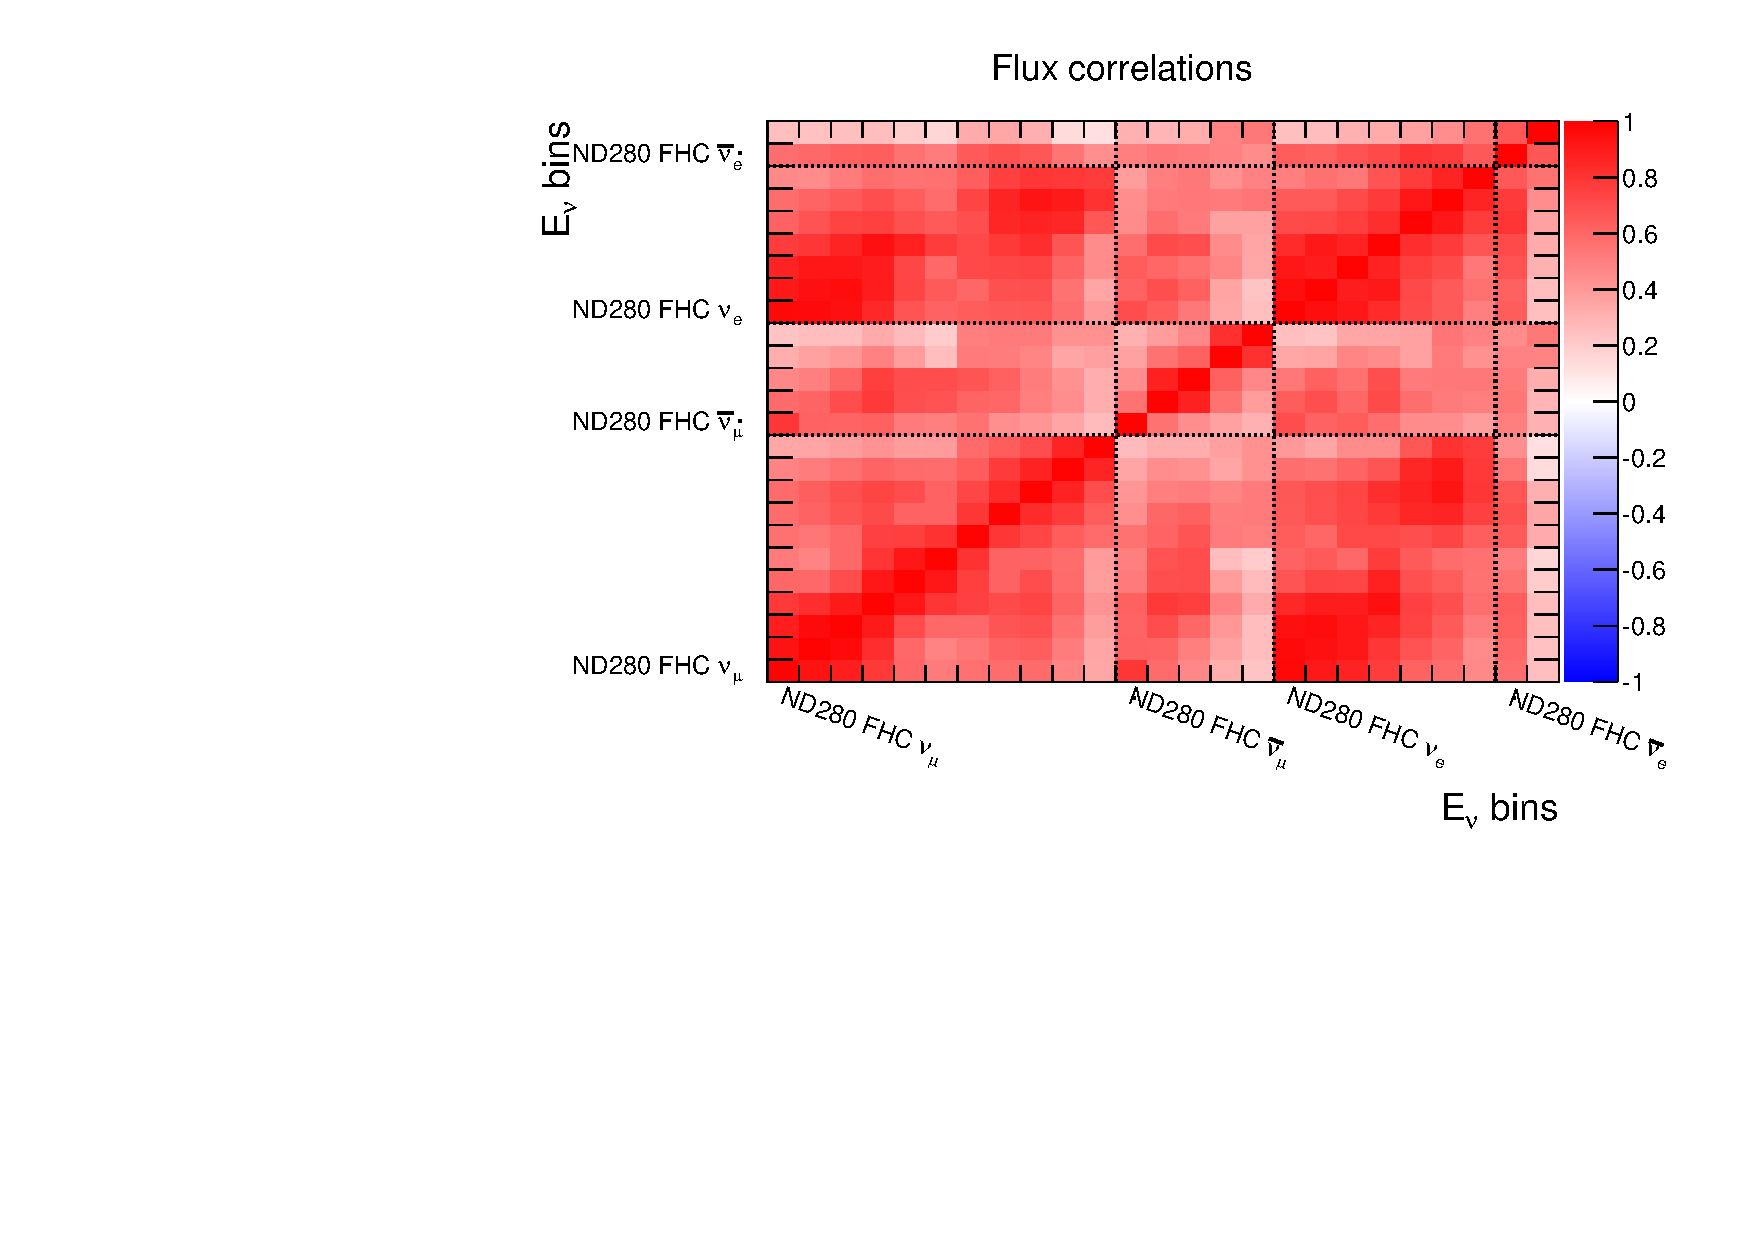
\includegraphics[width=0.8\textwidth]{T2K-TN-254/images/systematics/Flux.pdf} \\
  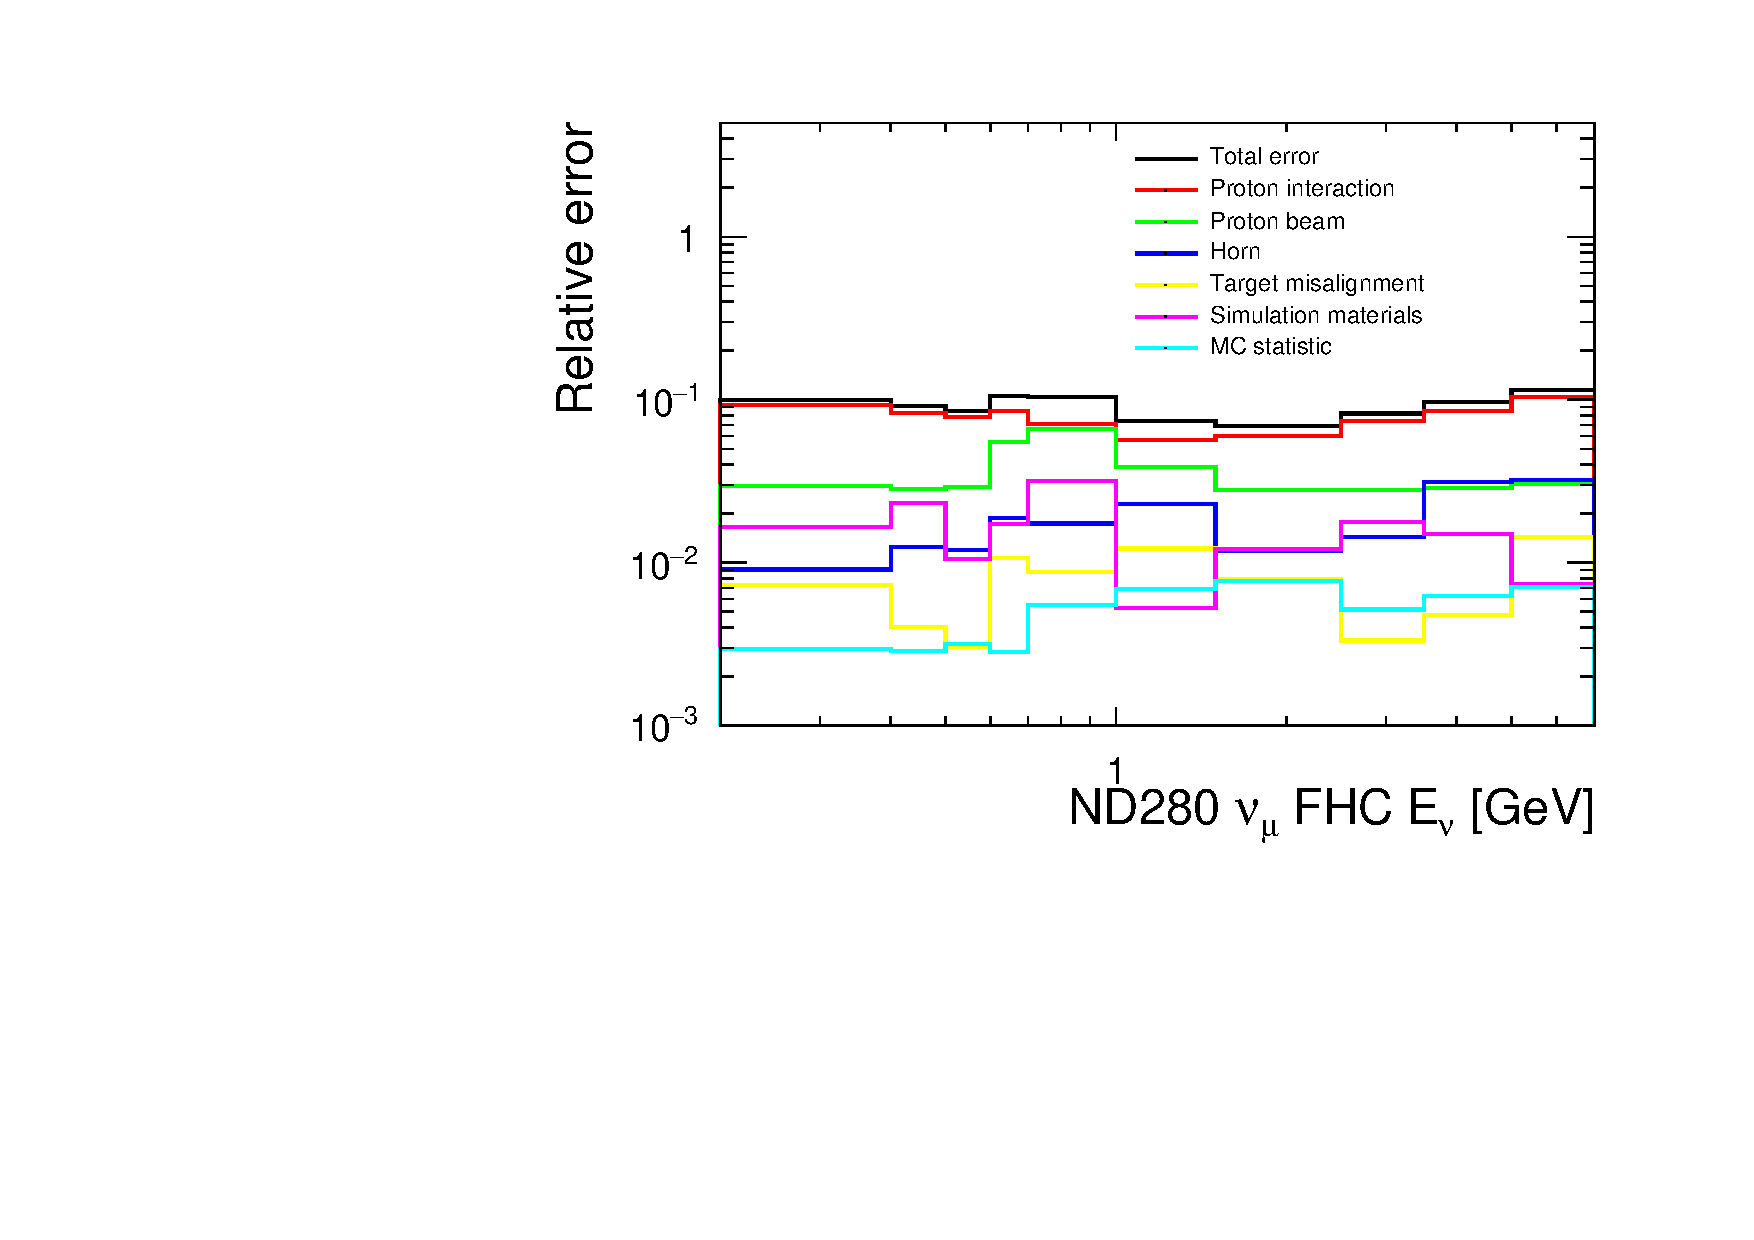
\includegraphics[width=0.8\textwidth]{T2K-TN-254/images/systematics/DiagError.pdf}
  \caption[T2K flux uncertainty and correlations across true energy
  bins in at ND280 and at SK]{\textbf{\textit{Top:}} The \Gls{TK} flux
    uncertainty correlations across true energy bins in for \Gls{ND}
    and \Gls{SK}, while running in \Gls{FHC} and \Gls{RHC} modes, for
    \Gls{numu}, \Gls{anumu}, \Gls{nue} and \Gls{anue}.
    \textbf{\textit{Bottom:}} The diagonal uncertainty for \Gls{numu}
    neutrinos in \Gls{FHC} at the \Gls{ND}. Both extracted from
    \Gls{TK} beam working group
    inputs~\cite{TomislavVladisavljevicFluxTuning2017,MarkHartzFluxUncertainty2017}.}
  \label{fig:fluxsystematics}
\end{figure}

As can be seen in Figure~\ref{fig:fluxsystematics}, the flux
uncertainty is expected to be around $10\%$.

Note that the flux uncertainty was constructed for \Gls{FGD} neutrino
interactions. The photons, on the other hand, can come from regions
far from the \Gls{FGD} central region. Following what was done in
\cite{MarkScott2013}, the conclusion was that the error should not be
increased by more than $5\%$ for \Gls{ECal} interactions. The increase
of the error is considered negligible compared to other effects taken
into account here.

Another motivation for not inflating the flux error is that the
photons do not come from very far from the tracker region, as can be
seen in Appendix~\ref{app:oofvphoton}. The conversion length of the
photons in the \Gls{ECal} ($10.4\text{~cm}$) is much shorter than for
a standard scintillator ($41.1\text{~cm}$), so it is not expected
that the \Gls{OOFV} neutrino interactions come from far regions such
as the \Gls{SMRD}.

The \Gls{PDF} (for Probability Density Function) of the number of
selected events is shown in Figure~\ref{fig:fluxsystematicspdf}.

\begin{figure}[ht]
  \begin{adjustbox}{center}
    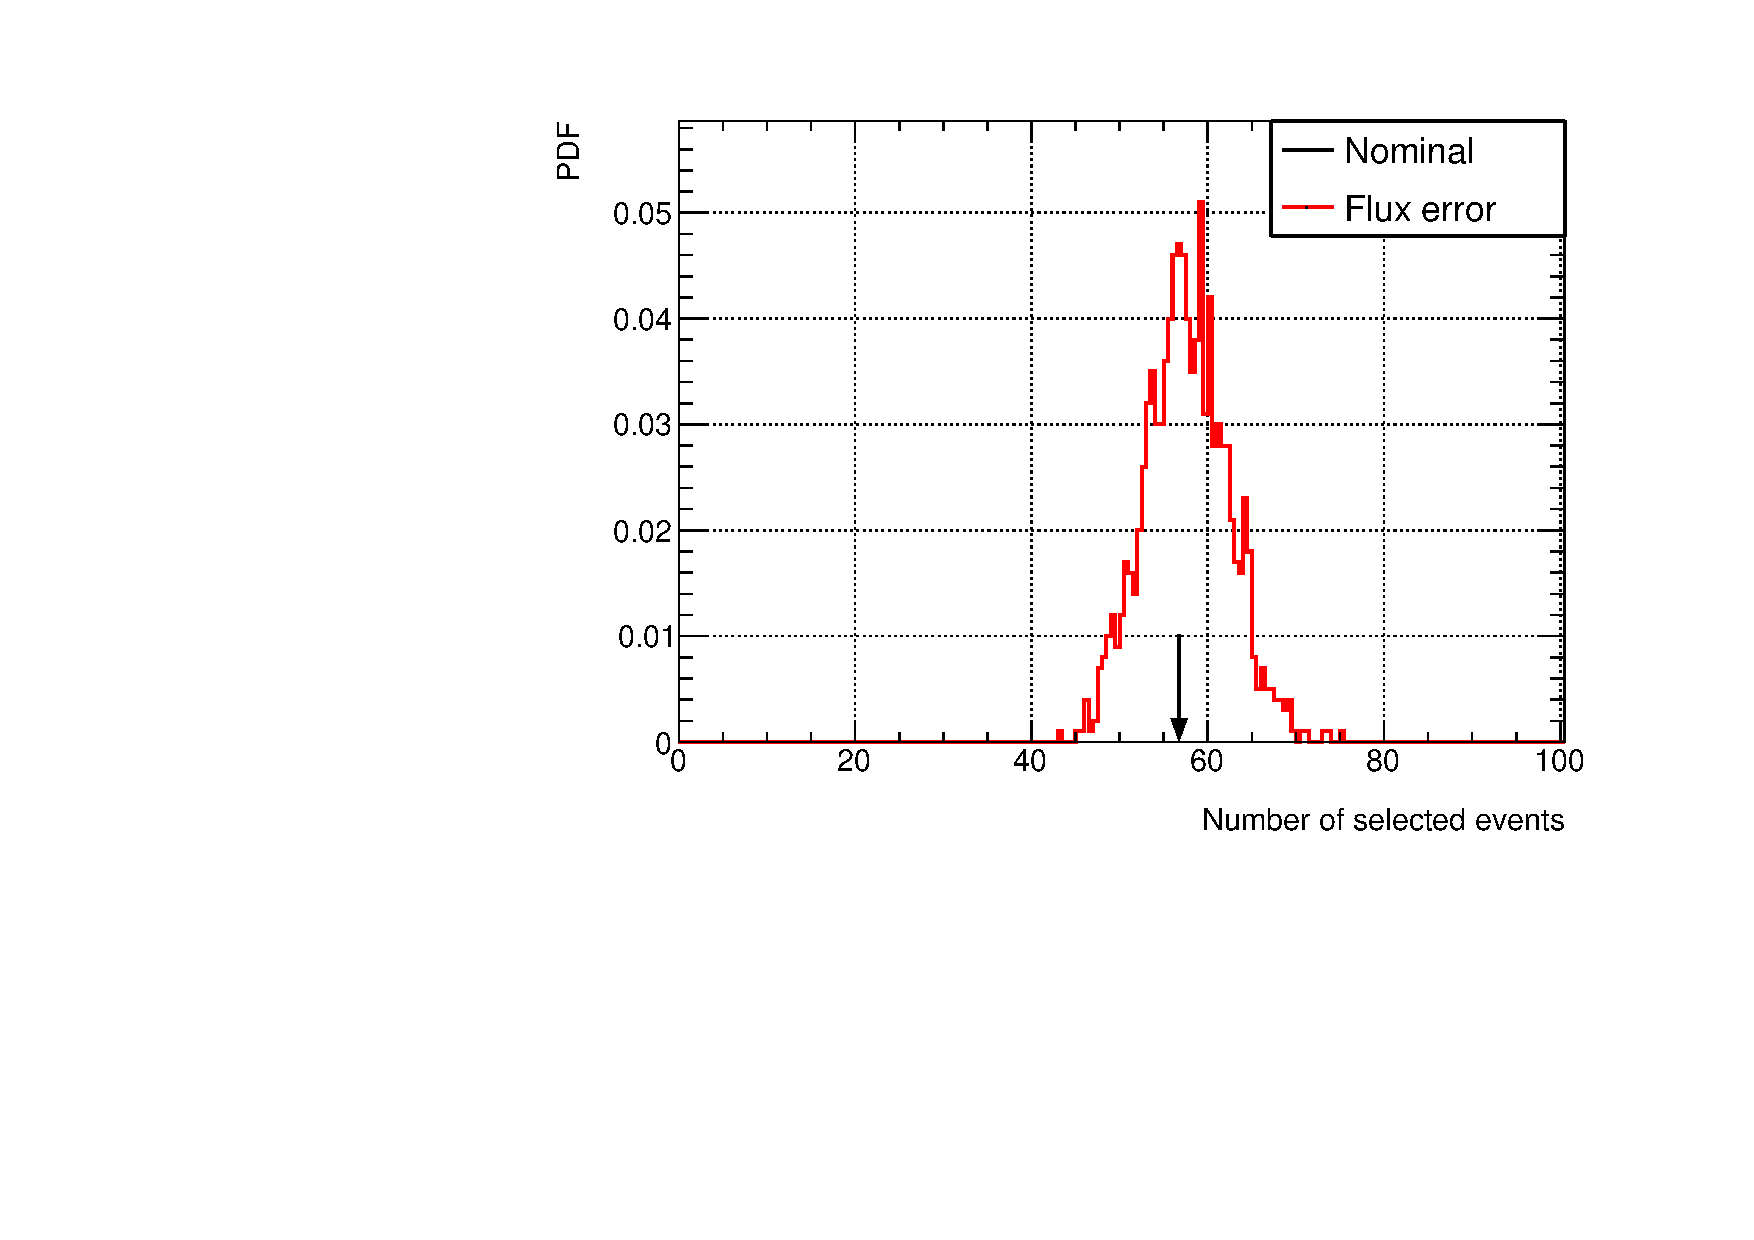
\includegraphics[width=0.8\textwidth]{images/NCg/Flux.pdf} 
  \end{adjustbox}
  \caption[Effect of the flux uncertainty on the number of selected
  events]{Effect of the flux uncertainty on the number of selected
    events. The nominal central value for \Gls{MC} is indicated by the
    arrow.}
  \label{fig:fluxsystematicspdf}
\end{figure}


%%% Local Variables:
%%% mode: latex
%%% TeX-master: "Thesis"
%%% End:
\clearpage

\section{Cross section systematic uncertainties}
\label{sec:xsecsyst}

The cross section uncertainties were propagated using the
\texttt{\Gls{T2KReWeight}} package~\cite{t2kreweight}, which modifies
the relative importance of the neutrino events based on a change of the
underlying cross section model.

\subsection{Cross section uncertainty on primary processes}
\label{subsec:primaryprocessuncertainty}
In this section, the cross section uncertainties on primary processes
are explained. The main background of the analysis comes from \gls{piz}
\Gls{NC} \Gls{RES} (resonant) interactions. There are a lot of vetoes
in the selection which remove muons from charged current interactions
and the second decay photons from the \Gls{piz}. All the cross section
systematic errors propagated are the same as those that were recently
used for the near detector fits supporting the oscillation analysis
in~\cite{Abe:2017vif} and in Chapter~\ref{chap:banff}.

Even if the \Gls{CCQE} processes are dominant at \Gls{TK} energies,
their impact on the analysis is minimal, since they only contribute
marginally to the selection of events as can be seen in
Table~\ref{tab:reaction}, standard cross section errors were
nevertheless propagated and will be explained here.

\subsubsection{Free nucleon resonant interaction uncertainties}
\label{subsubsec:freeres}
There are three uncertainties related to the \Gls{RES}
interactions. All of them are parameters of the Rein and Sehgal
model~\cite{Rein1,Rein2}.

\paragraph{Resonant axial mass}
This parameter controls the axial mass ($M_A^{\text{RES}}$). This is
one of the fundamental inputs for the cross section calculation
related to the form factor. \Gls{TK} now uses a new form factor
compared to the original one from Rein and Sehgal, which has the
form~\cite{PhysRevD.77.053001}:
\begin{equation}
  \label{eq:ffres}
  \sigma_{\text{RES}} \propto  C^A_5(Q^2)=\frac{C^A_5(0)}{\left(1+\frac{Q^2}{\left.M_A^{\text{RES}}\right.^2}\right)^2}.
\end{equation}
Where the linear dependence of the neutrino cross section
($\sigma_{\text{RES}}$) to the axial form factor ($C^A_5$) is made
explicit. In this equation, $M_A^{\text{RES}}$ is the axial mass
(which is the equivalent for \Gls{RES} cross section to the \Gls{CCQE}
$M_A^{\text{QE}}$ described in Section~\ref{subsec:ccqe}), and $Q^2$
(see Footnote~\ref{ftn:qsquare} on page~\pageref{ftn:qsquare}) is the
momentum transfer.

\paragraph{Resonant axial form factor at \texorpdfstring{$Q^2=0$}{TEXT}}
In Equation~\ref{eq:ffres}, the parameter $C^A_5(0)$ is also an
uncertainty, which acts on the total normalisation of the \Gls{RES}
events.

\paragraph{Isospin 1/2 background} The background component refers to
the non-resonant component contribution of the cross section as
described in Section~\ref{subsec:res}.

\paragraph{Tuning and uncertainty}
Several tunings of these parameters are done using different
combinations of the available data (bubble chamber), and using
channels that are sensitive or not to the background
term~\cite{TN315}.

The errors used are listed in Table~\ref{tab:reserror}.

\begin{table}[ht]
  \begin{adjustbox}{center}
    \begin{tabular}{cccccc}
      \toprule
      Parameter & Value & Error & \multicolumn{3}{c}{Correlation} \\
                &       &       & $M_A$   & $C_5^A$ & $I_{1/2}$ \\
      \midrule
      $M_A$     & 1.07  & 0.15  & $1$     & $-0.83$ & $-0.01$   \\
      $C_5^A$   & 0.96  & 0.15  & $-0.83$ & $1$     & $-0.31$   \\
      $I_{1/2}$ & 0.96  & 0.40  & $-0.01$ & $-0.31$ & $1$       \\
      \bottomrule
    \end{tabular}
  \end{adjustbox}
  \caption[Neutrino RES error used in the analysis]{Neutrino \Gls{RES}
    errors used in the analysis, reproduced from~\cite{TN315}.}
  \label{tab:reserror}
\end{table}

\subsubsection{Nuclear resonant interaction uncertainty, the
  \Gls{MiniBooNE} \texorpdfstring{$NC1\pi^{0}$}{TEXT} fits}
\label{subpar:miniboonefits}
Due to the relative importance of \Gls{piz} in the analysis, it was
decided to add additional parameters to properly deal with the
uncertainties coming from these events where a \piz was created. It
should be noted that most of these backgrounds are from resonant
interactions and single \Gls{piz} production as can be seen in the
previous section
(Tables~\ref{tab:reaction}~and~\ref{tab:topo}). Furthermore, in
Figures~\ref{fig:pizeff1}~and~\ref{fig:pizeff2}, one can see that the
efficiency in selecting these \Gls{piz} from resonant interactions is
not flat.  Therefore, any uncertainty on the \Gls{piz} background that
creates a shape difference in the pion kinetic space is expected to
have a significant importance in the overall systematic error
budget. These parameters are relevant since none of the previously
described parameters has the ability to change the pion momentum
distribution. This can be seen in Figure~\ref{fig:currenterrors},
where the neutral pion (\Gls{piz}) measurement was from
\Gls{MiniBooNE}~\cite{AguilarArevalo:2009ww} and compared to the
\Gls{NEUT} prediction and errors.

Based on this study, two parameters were re-introduced from cross
section parametrisation (identical to the ones used in Section B.3
of~\cite{T2KLong}). The reason is that the errors on the pion
kinematics produced by the cross section parameter described earlier
do not cover all the data points and a shape discrepancy can be
seen. Note that all the plots and studies were realised with the
newly-released \Gls{NUISANCE}~\cite{NUISANCE2017}.

The \Gls{TK} pion model (which is the Rein and Sehgal
model~\cite{Rein1,Rein2} with the parameters: axial mass,
normalisation of the form factor and isoscalar background free) is
fitted using the bubble chamber data, and the reasons why this
under-coverage could happen are multiple: for example a problem with
\Gls{FSI}, but also the Pion-less Delta decay or any other nuclear
effects (such as the one discussed in the Section~\ref{subsec:res})
that makes the extrapolation from a single nucleon to nuclear target
wrong. Note that all the parameters described above are designed to
act on the leading muon kinematics in the Charged Current resonant
channels.

In most of the extended models that deal with resonant interactions in
nuclear media, the modifications that arise are dependent on the
momentum of the resonance (Delta width), so a parameter that modifies
the shape of the $W$ distribution is a fairly natural way to account
for differences arising from nuclear correction. The parameters as
function of $Q^2$ have more impact on the leading lepton. If one looks
at the pion momentum, these parameters are acting as normalisation and
cannot change the shape of the pion momentum.

For the purpose of the analysis, the \Gls{MiniBooNE} \Gls{NC}\gls{piz}
momentum distribution~\cite{AguilarArevalo:2009ww} was fitted using
the Delta width and position of the Breit-Wigner distribution.

In the \Gls{MiniBooNE} fits, the normalisation of the data is left
free as most of the existing bubble chamber data are already
constraining the normalisation of the nucleon level resonant processes
and were explicitly tuned to accommodate other \Gls{MiniBooNE}
\Gls{CC} and \Gls{NC} measurement normalisations~\cite{TN315}.

Similarly, the \Gls{FSI} (for which the systematic error effects are
not displayed in any of the plots in this section) can also change the
normalisation (but not the shape of the pion momentum). This is
because it is not simple to code a reweighting scheme which changes
the shape of the kinematics of the pions when they undergo the
\Gls{FSI}. Therefore, given that the normalisation of the data is a
convolution of a number of non trivial parameters, it was chosen to
leave the normalisation free, and the aim of this fit is solely to be
able to reproduce \Gls{MiniBooNE} pion kinetical shape with sensible
errors.

After doing the fit, one gets the result for the parameters listed in
Table~\ref{tab:fitresult}. In this case, only the two Delta parameters
were fitted, while the other parameters were fixed at their initial
tuned values.

\begin{table}[ht]
  \begin{adjustbox}{center}
    \begin{tabular}{ccc}
      \toprule
      Parameter & Prior & Uncertainty \\
      \midrule
      $\Delta$ mass mean  & -0.002 & 0.004 \\
      $\Delta$ mass width & -0.26  & 0.14  \\
      \bottomrule
    \end{tabular}
  \end{adjustbox}
  \caption[MiniBooNE $p_{NC\pi^{0}}$ shape-only fit
  result]{\Gls{MiniBooNE} $p_{NC\pi^{0}}$ shape-only fit result.}
  \label{tab:fitresult}
\end{table}

The plots in Figure~\ref{fig:miniboonepostfit} show the error coverage
one gets after generating toy with the errors from
Table~\ref{tab:fitresult} and the all the standard errors
from~\cite{TN193}. The Figure~\ref{fig:miniboonepostfitcoh} shows the
same distribution with an increased \Gls{NC} coherent uncertainty from
$30\%$ to $100\%$. This was done to try to accommodate data~/~\Gls{MC}
differences in the forward region, which is expected to be purer in
coherent interactions as illustrated on
Figure~\ref{fig:miniboonebreakdown}.


\begin{figure}[ht]
  \center
  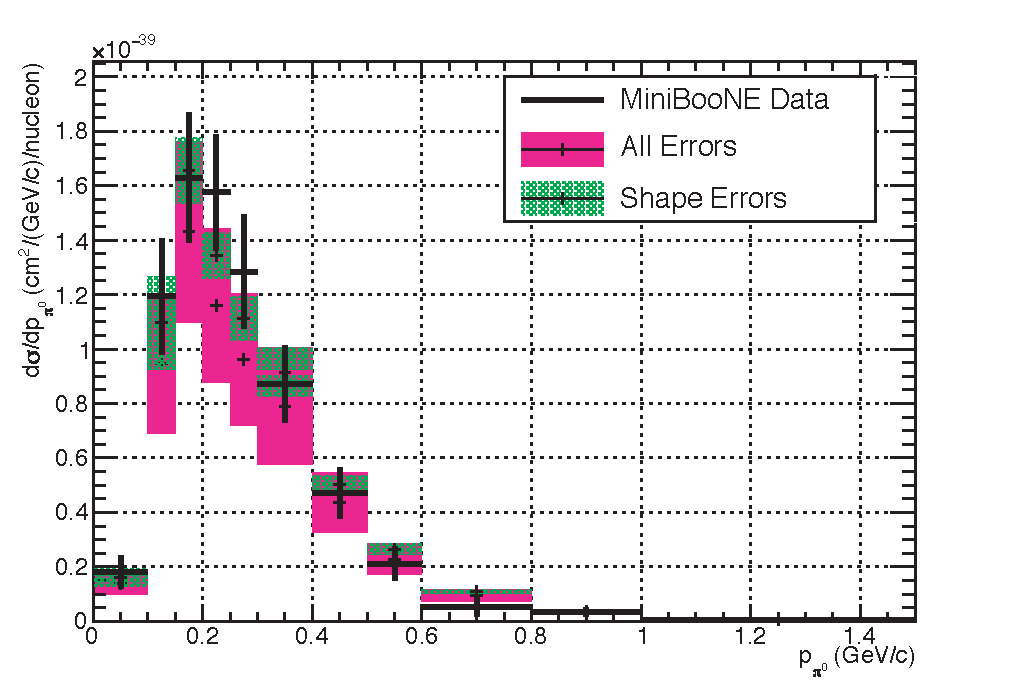
\includegraphics[width=0.8\textwidth]{T2K-TN-254/images/systematics/MB_NC1Pi0_pPi0_nu_curr_good.pdf}\\ %%
  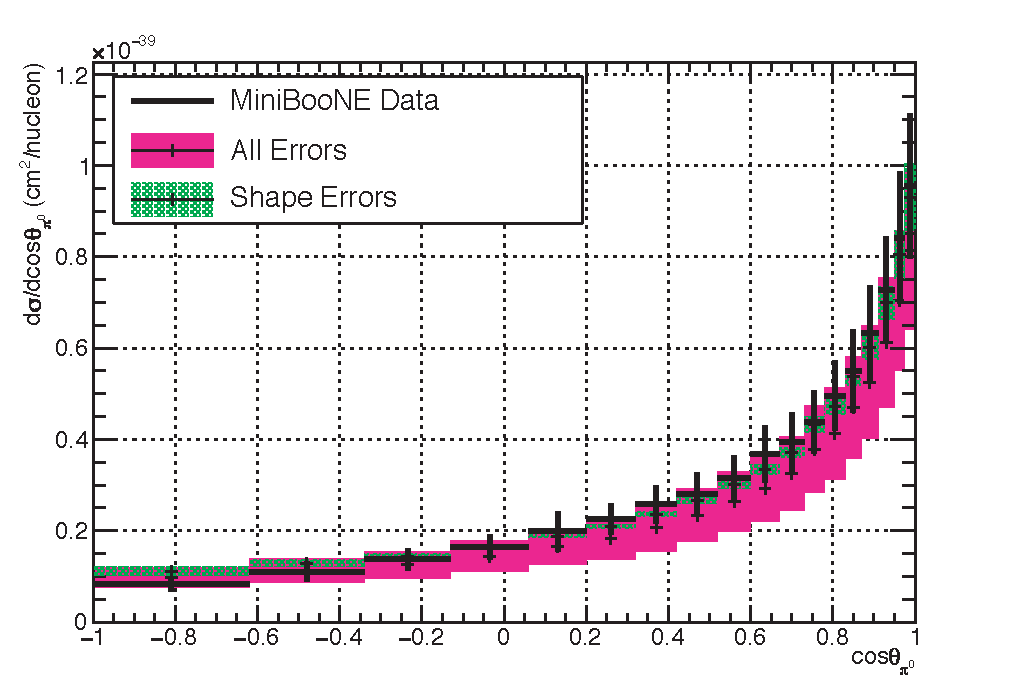
\includegraphics[width=0.8\textwidth]{T2K-TN-254/images/systematics/MB_NC1Pi0_ctPi0_nu_curr_good.pdf} %%
  \caption[MiniBooNE error coverage from current
  parametrisation]{\Gls{MiniBooNE} error coverage from standard
    parametrisation~\cite{TN315} (Table~\ref{tab:reserror}). The black
    line shows the \Gls{MiniBooNE} neutrino mode \Gls{NC}\gls{piz}
    data~\cite{AguilarArevalo:2009ww}, magenta boxes \Gls{NEUT}
    predictions with errors, overlayed green boxes are shape only
    variations from \Gls{NEUT}. \textbf{\textit{Top:}} Pion momentum
    distribution. \textbf{\textit{Bottom:}} Pion angular
    distribution.}
  \label{fig:currenterrors}
\end{figure}

\begin{figure}[ht]
  \center
  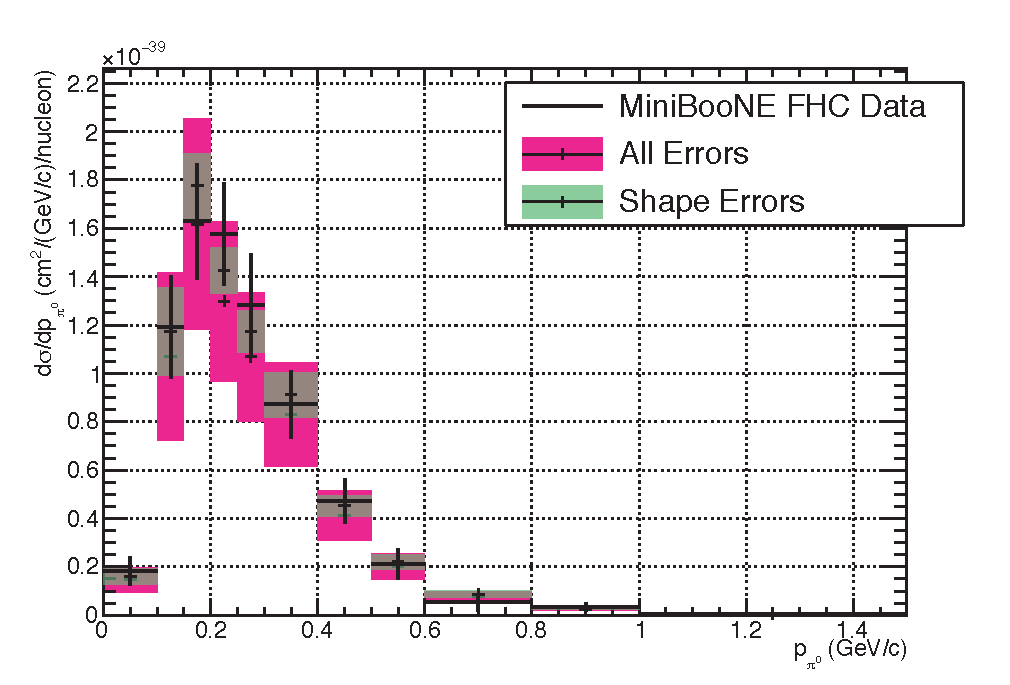
\includegraphics[width=0.8\textwidth]{T2K-TN-254/images/systematics/MB_NC1pi0_1Dppi0_fhc_nu_1WShape_good.pdf}\\ %%
  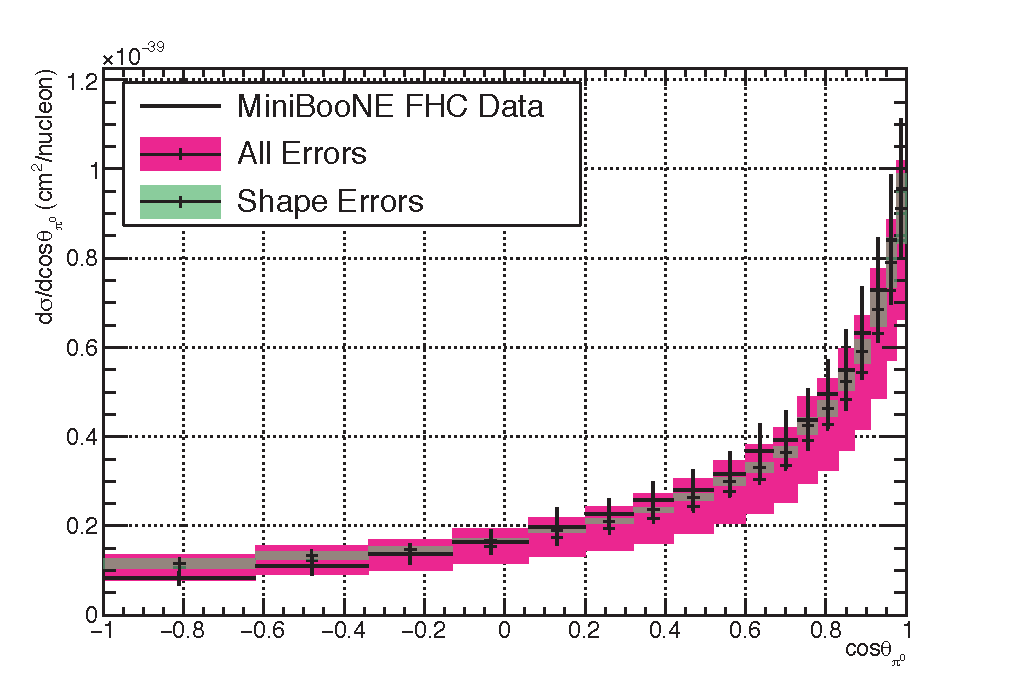
\includegraphics[width=0.8\textwidth]{T2K-TN-254/images/systematics/MB_NC1pi0_1Dcospi0_fhc_nu_1WShape_good.pdf} %%
  \caption[MiniBooNE error coverage using the fitted
  errors]{\Gls{MiniBooNE} error coverage using the fitted errors from
    standard parametrisation~\cite{TN315} (Table~\ref{tab:reserror})
    and $W$-shape error (Table~\ref{tab:fitresult}). The black line
    shows the \Gls{MiniBooNE} neutrino mode \Gls{NC}\gls{piz}
    data~\cite{AguilarArevalo:2009ww}, magenta boxes \Gls{NEUT}
    predictions with errors, overlayed green boxes are shape only
    variations from \Gls{NEUT}. \textbf{\textit{Top:}} Pion momentum
    distribution. \textbf{\textit{Bottom:}} Pion angular
    distribution.}
  \label{fig:miniboonepostfit}
\end{figure}


\begin{figure}[ht]
  \center
  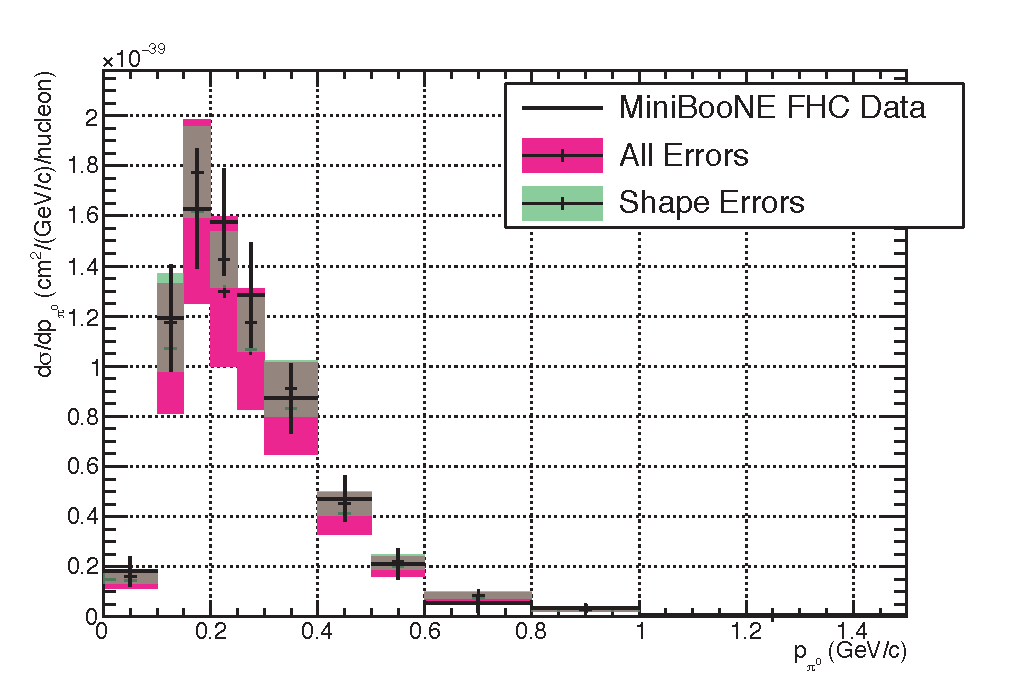
\includegraphics[width=0.8\textwidth]{T2K-TN-254/images/systematics/MB_NC1pi0_1Dppi0_fhc_nu_1WShape_highNCCoh_good.pdf} \\ %%
  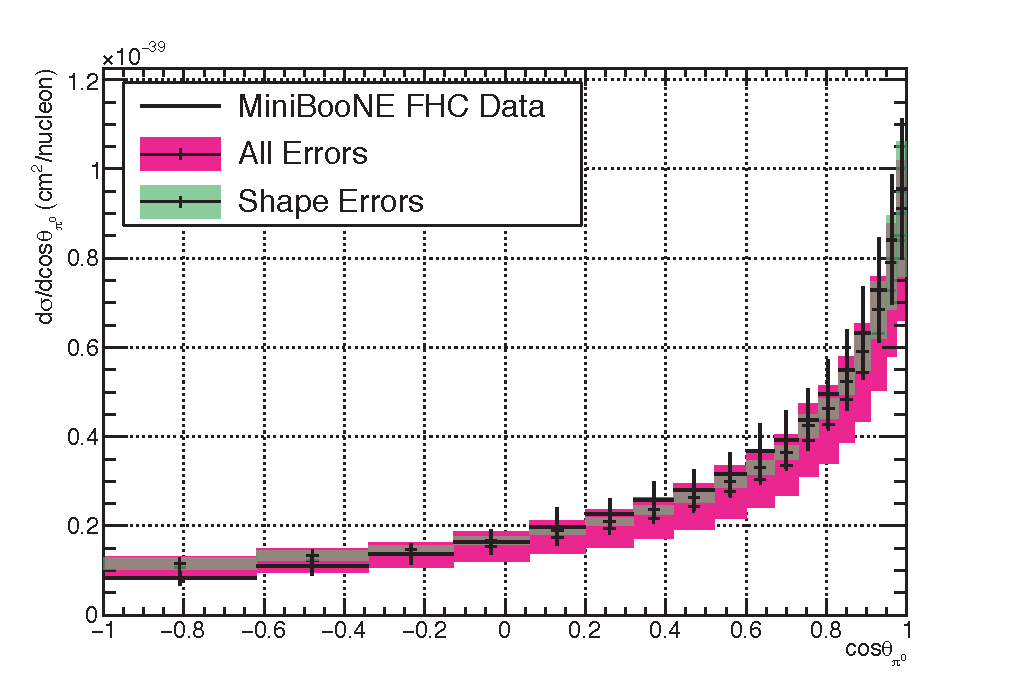
\includegraphics[width=0.8\textwidth]{T2K-TN-254/images/systematics/MB_NC1pi0_1Dcospi0_fhc_nu_1WShape_highNCCoh_good.pdf} %%
  \caption[MiniBooNE error coverage using the fitted errors and an
  additional error for NC COH events]{\Gls{MiniBooNE} error coverage
    using the fitted errors from standard parametrisation~\cite{TN315}
    (Table~\ref{tab:reserror}) and from $W$-shape error
    (Table~\ref{tab:fitresult}) with a $100\%$ error on \Gls{NC}
    coherent interaction The black line shows the \Gls{MiniBooNE}
    neutrino mode \Gls{NC}\gls{piz} data~\cite{AguilarArevalo:2009ww},
    magenta boxes \Gls{NEUT} predictions with errors, overlayed green
    boxes are shape only variations from
    \Gls{NEUT}. \textbf{\textit{Top:}} Pion momentum
    distribution. \textbf{\textit{Bottom:}} Pion angular
    distribution.}
  \label{fig:miniboonepostfitcoh}
\end{figure}

\begin{figure}[ht]
  \center
  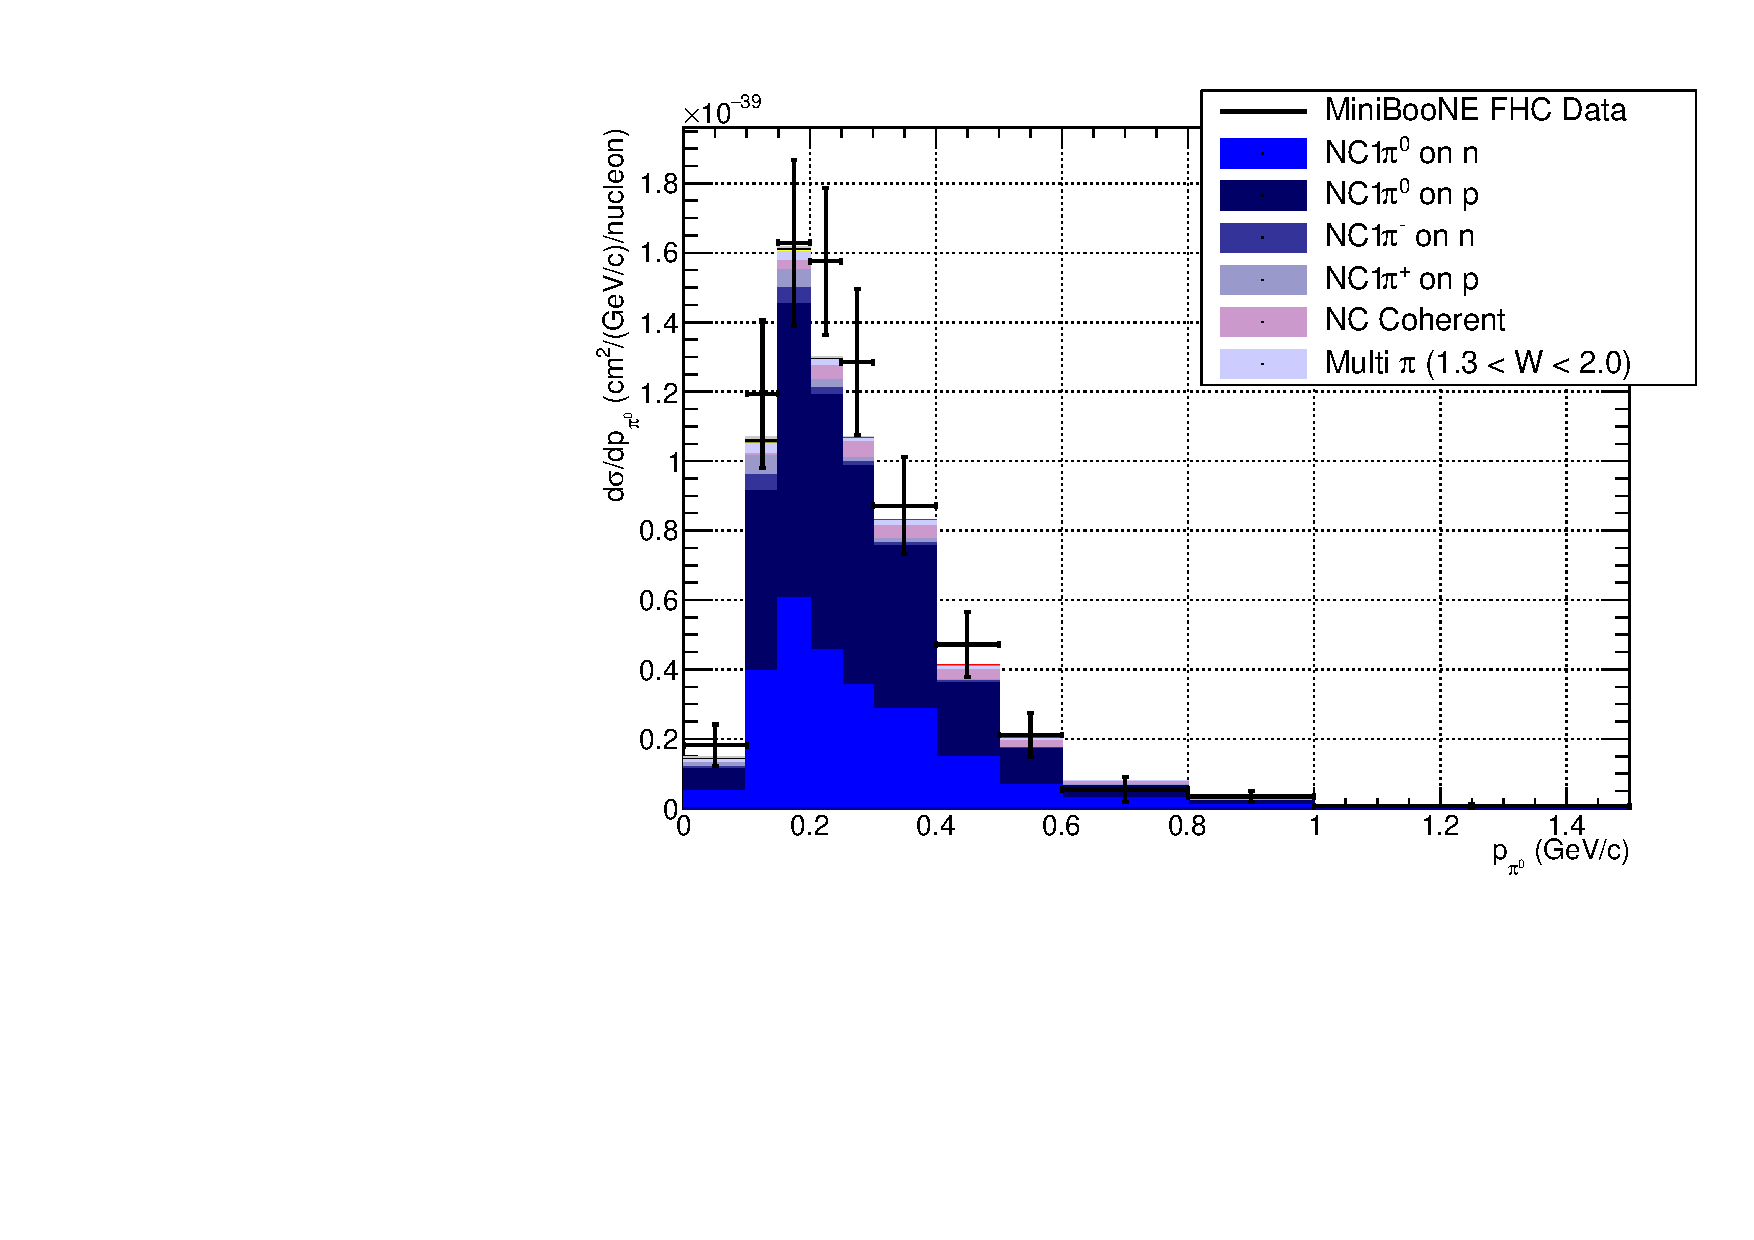
\includegraphics[width=0.8\textwidth]{T2K-TN-254/images/systematics/MB_NC1Pi0_comp_ppi.pdf} %%
  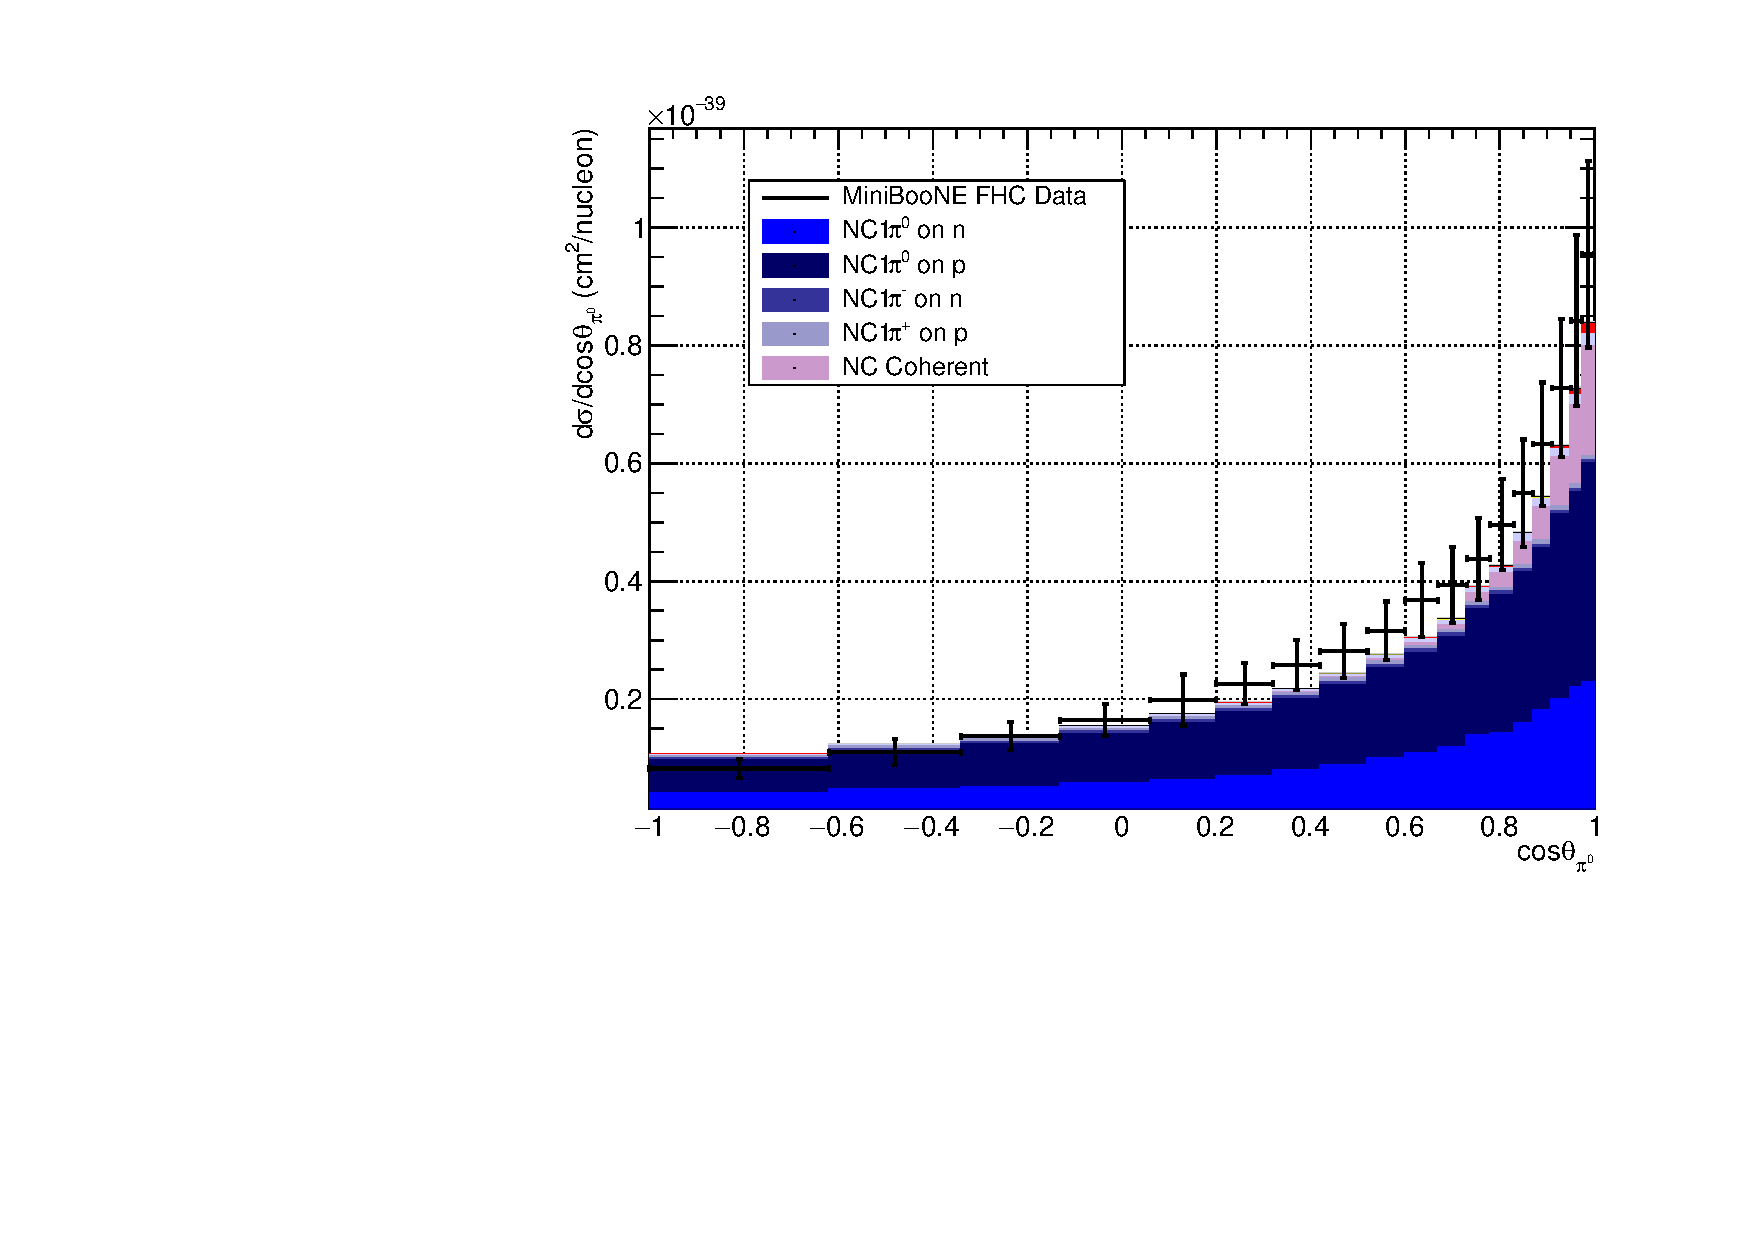
\includegraphics[width=0.8\textwidth]{T2K-TN-254/images/systematics/MB_NC1Pi0_comp_cospi.pdf} %%
  \caption[MiniBooNE NC$\pi^0$ differential
  distribution]{\Gls{MiniBooNE} \Gls{NC}\gls{piz} differential
    distribution, top: $p_{\pi^{0}}$, bottom:
    $\cos(\theta_{\pi^{0}})$, broken down by \Gls{NEUT} reaction
    modes, the central values and are the same as for
    \ref{fig:miniboonepostfitcoh}.}
  \label{fig:miniboonebreakdown}
\end{figure}

In the case of the \Gls{OOFV} background interactions, they mostly are
from \Gls{RES} interactions, as can be seen in
Tables~\ref{tab:reaction}~and~\ref{tab:target}. The same effects as
described before are also valid so one could wonder if having a carbon
measurement is enough. However, given that there is no
\Gls{NC}\gls{piz} measurement on target other than carbon (and Argon
with \Gls{ArgoNeuT}~\cite{Acciarri:2015ncl}) where the \Gls{piz}
kinematics are available, and the size of the detector error, it was
considered that the differences in uncertainty between carbon and
other nuclear targets should be negligible and thus the uncertainties
described above were applied to the \Gls{OOFV} interactions.

\clearpage

\subsubsection{Relativistic Fermi Gas parameters}
The \Gls{RFG} model is dependent on two fundamental parameters. Both
of them can be determined via electron
scattering~\cite{Alvarez-Ruso:2017oui}.

The first parameter is the Fermi momentum, this quantity is determined
by the width of the elastic peak. The second parameter is the binding
energy, which is determined by the position of the elastic peak. This
quantity corresponds to the energy needed to extract a nucleon from
the Fermi sea.

Unfortunately, even with very accurate electron scattering
measurements, it is hard to find values for these two parameters which
can explain all the electron scattering data~\cite{TN315}, indicating
a deficiency in the model.

The values and uncertainties that are used at \Gls{TK} are listed in
Table~\ref{tab:rfgerror}

\begin{table}[ht]
  \begin{adjustbox}{center}
    \begin{tabular}{cccc}
      \toprule
      Parameter & Value (carbon) & Value (oxygen) & Error \\
      \midrule
      Fermi momentum $p_F$ & $217\text{~MeV}$ & $225\text{~MeV}$ & $31\text{~MeV}$ (flat prior)\\
      Binding energy $E_B$ & $25\text{~MeV}$  & $27\text{~MeV}$  & $9\text{~MeV}$  (flat prior)\\
      \bottomrule
    \end{tabular}
  \end{adjustbox}
  \begin{center}
    \caption[Neutrino RFG errors]{Neutrino \Gls{RFG} errors used
      in the oscillation analysis, reproduced from~\cite{TN315}}
    \label{tab:rfgerror}
  \end{center}
\end{table}

Note that decreasing the $E_B$ parameter ``opens up'' parameter space
(as more events are allowed), and creating a reweighting scheme for
these parameters is not a trivial problem and can lead to significant
bias~\cite{TN315}.

\subsubsection{CCQE Form factor}
Based on bubble chamber data~\cite{ANLCCQE,BNLCCQE,CERNCCQE}, the
\Gls{CCQE} form factor error that is used for the propagation is
$5.8$~\%.

\subsubsection{Multi nucleons}
A $29.5$~\% normalisation uncertainties is assumed for multi-nucleons
events, this comes from analysis from the
\Gls{MINERVA}~\cite{MinervaNuCCQE} and
\Gls{MiniBooNE}~\cite{MiniBooNENuCCQE} experiments.

\subsection{Electron neutrino error}
\label{subsec:electnuerror}
The traditional error for the electron neutrino cross section error is
parametrised as an error on the ratio
$\frac{\sigma_{\text{CC~inc~}\nu_e}}{\sigma_{\text{CC~inc~}\nu_\mu}}$
and similarly for anti-neutrinos. This is admitted to be of the order
of $3\%$, with a $50\%$ correlation for neutrino and anti-neutrino
based on studies in~\cite{Day:2012gb}.

\subsection{Other cross section uncertainty}
\label{subsec:othercrosssection}
Other uncertainties were propagated on the \Gls{DIS} and \Gls{COH}
events. In the case of \Gls{DIS} and \Gls{SIS} events, the scheme is
to reweight the normalisation of the events with an error of the form:
\begin{equation}
  \label{eq:diserror}
  \delta_{\sigma}=\frac{0.4}{E_\nu}
\end{equation}

Which gives an error of $10\%$ at $4$~GeV as was observed
in~\cite{Adamson:2009ju}.

The \Gls{NC} and \Gls{CC} \Gls{COH} events have a normalisation error
of $100\%$ as explained in the previous section.

\subsection{Final State Interactions}
\label{subsec:fsiuncertainty}
Final state interactions denote all the hadron interactions in the
nucleus that happen after the primary neutrino interaction. For
example, if a resonant process happens and creates a pion, this pion
is inside the nucleus and can reinteract in the nucleus. The effect of
the \Gls{FSI} is to generally change the topology of the event (bias
towards lower energy for the pion, absorption of the pion, charge
exchange). However, as discussed earlier, these changes in the shape
have no error (only a normalisation error). For each \Gls{NEUT}
interaction channel of the pion inside the nucleon, an uncertainty is
computed. All the parameters and errors are given in the
Table~\ref{tab:fsiuncertainty}.

\begin{table}[ht]
  \center
  \begin{tabular}{lc}
    \toprule
    Systematic & Relative uncertainty \\
    \midrule
    Pion absorption             & $50\%$  \\
    Low energy charge exchange  & $50\%$  \\
    Low energy quasi elastic    & $50\%$  \\
    Inelastic scattering        & $50\%$  \\
    High energy charge exchange & $30\%$  \\
    High energy quasi elastic   & $30\%$  \\
    \bottomrule
  \end{tabular}
  \caption[FSI parameters and uncertainties]{\Gls{FSI} parameters and
    uncertainties.}
  \label{tab:fsiuncertainty}
\end{table}

For this analysis, the ``16 throws'' method was used. The idea is that
it is sufficient to use sixteen different parameter sets for the
\Gls{FSI} parameters to estimate the systematic error from
\Gls{FSI}. These parameter sets have been detailed in~\cite{TN108} and
are reproduced in Table~\ref{tab:16throws}. The effect of applying
this reweighting is shown in Figure~\ref{fig:fsierror}.

\begin{table}[ht]
  \center
  \begin{tabular}{cccccccc}
    \toprule
    Set & \multicolumn{6}{c}{Parameters} \\ 
        & \multicolumn{2}{c}{Quasi elastic} & Inelastic & Pion       & \multicolumn{2}{c}{Charge exchange}\\
        & LowE  & HighE         & scattering& absorption & LowE &  HighE\\ \midrule
    Nominal  & 1.0  & 1.8   & 1      & 1.1   & 1.0  & 1.8    \\ \midrule
    15 & 0.6  & 1.1   & 1.5    & 0.7   & 0.5  & 2.3    \\
    16 & 0.6  & 1.1   & 1.5    & 0.7   & 1.6  & 2.3    \\
    17 & 0.7  & 1.1   & 1.5    & 1.6   & 0.4  & 2.3    \\
    18 & 0.7  & 1.1   & 1.5    & 1.6   & 1.6  & 2.3    \\
    19 & 1.4  & 1.1   & 1.5    & 0.6   & 0.6  & 2.3    \\
    20 & 1.3  & 1.1   & 1.5    & 0.7   & 1.6  & 2.3    \\
    21 & 1.5  & 1.1   & 1.5    & 1.5   & 0.4  & 2.3    \\
    22 & 1.6  & 1.1   & 1.5    & 1.6   & 1.6  & 2.3    \\ \midrule
    23 & 0.6  & 2.3   & 0.5    & 0.7   & 0.5  & 1.3    \\
    24 & 0.6  & 2.3   & 0.5    & 0.7   & 1.6  & 1.3    \\
    25 & 0.7  & 2.3   & 0.5    & 1.6   & 0.4  & 1.3    \\
    26 & 0.7  & 2.3   & 0.5    & 1.6   & 1.6  & 1.3    \\
    27 & 1.4  & 2.3   & 0.5    & 0.6   & 0.6  & 1.3    \\
    28 & 1.3  & 2.3   & 0.5    & 0.7   & 1.6  & 1.3    \\
    29 & 1.5  & 2.3   & 0.5    & 1.5   & 0.4  & 1.3    \\
    30 & 1.6  & 2.3   & 0.5    & 1.6   & 1.6  & 1.3    \\ \bottomrule
  \end{tabular}
  \caption[The ``16 throws'' parameter sets of the FSI parameters]{The
    ``16 throws'' parameter sets of the \Gls{FSI} parameters.}
  \label{tab:16throws}
\end{table}

\begin{figure}[ht]
  \center
  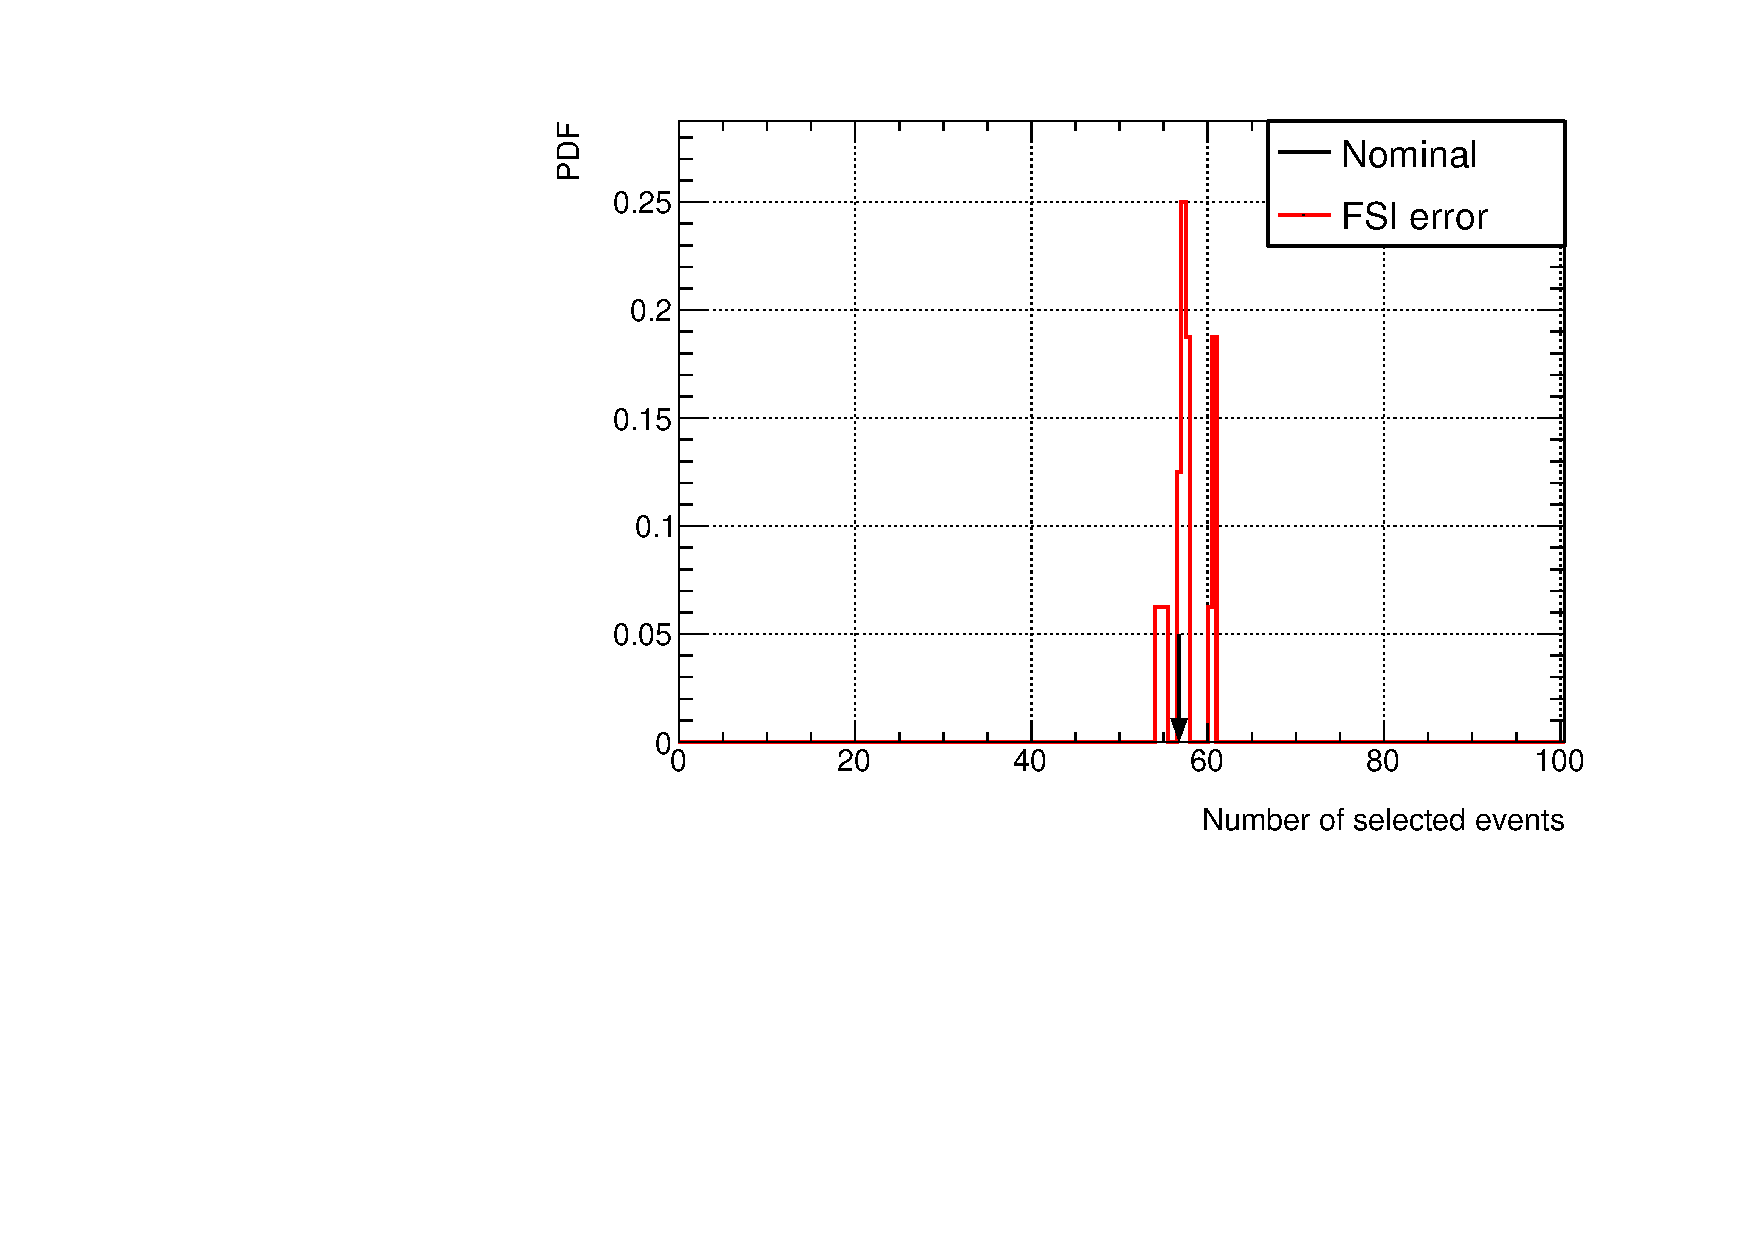
\includegraphics[width=0.8\textwidth]{images/NCg/FSI.pdf} 
  \caption[Effect of the pion FSI uncertainty on the number of
  selected events]{Effect of the pion \Gls{FSI} uncertainty on the
    number of selected events, using the ``16 throws method''. The
    nominal central value is indicated by the arrow.}
  \label{fig:fsierror}
\end{figure}

Some interactions creating these \Gls{piz} are on heavy elements, such
as the one on the aluminium of the support structure or the lead of
the \Gls{ECal}. Additionally, some interactions on the brass in the
\Gls{PD} can occur.

For the \Gls{FSI}, the \Gls{NEUT} program is used to predict the
pion-nuclear cross section on heavy targets and compared with the
available pion scattering data. A subset of these comparisons is shown
in Figure~\ref{fig:fsiheavy}, which comes from~\cite{FSITalk}, where
all of them are available. Most of the data points lie within the
current error budget, so the errors were not inflated. There is
currently no shape uncertainty for the \Gls{FSI}, and since the
\gls{piz} momentum efficiency is not flat (as can be seen in
Figures~\ref{fig:pizeff1}~and~\ref{fig:pizeff2}), this could lead to
an effect similar to the one described earlier with the Delta mass
parameter. However, \Gls{FSI} shape reweighting will not be done on an
acceptable timescale for the scope of this work; it was therefore
assumed that the normalisation error is sufficient to cover the error.


\begin{figure}[ht]
  \center
  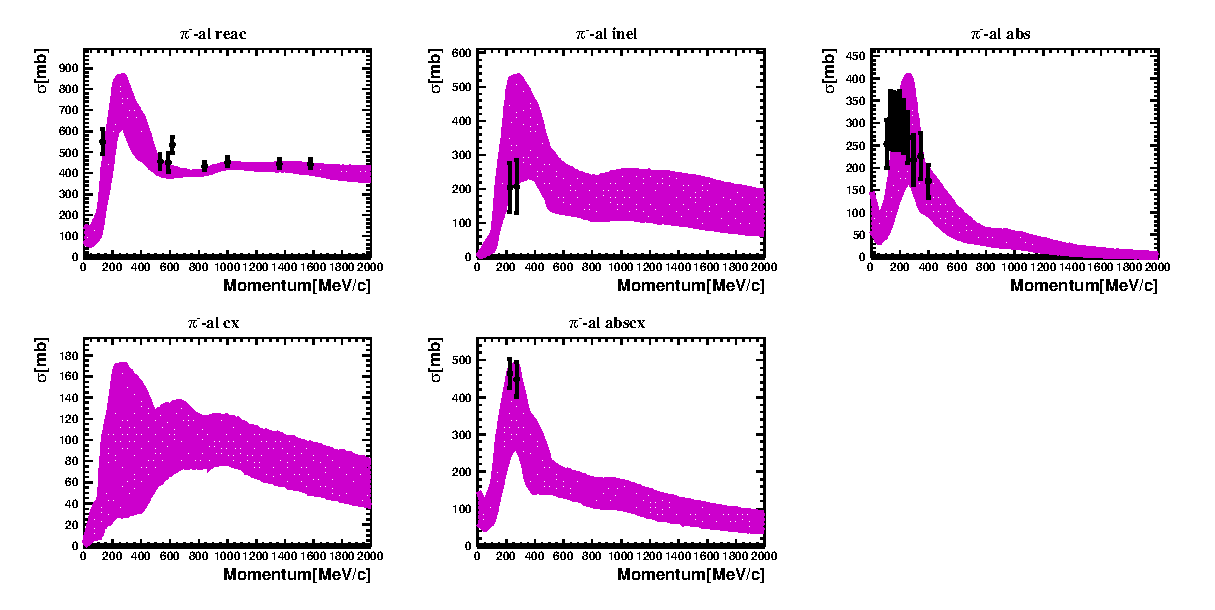
\includegraphics[width=0.9\textwidth]{T2K-TN-254/images/systematics/al_piM_all.eps}
  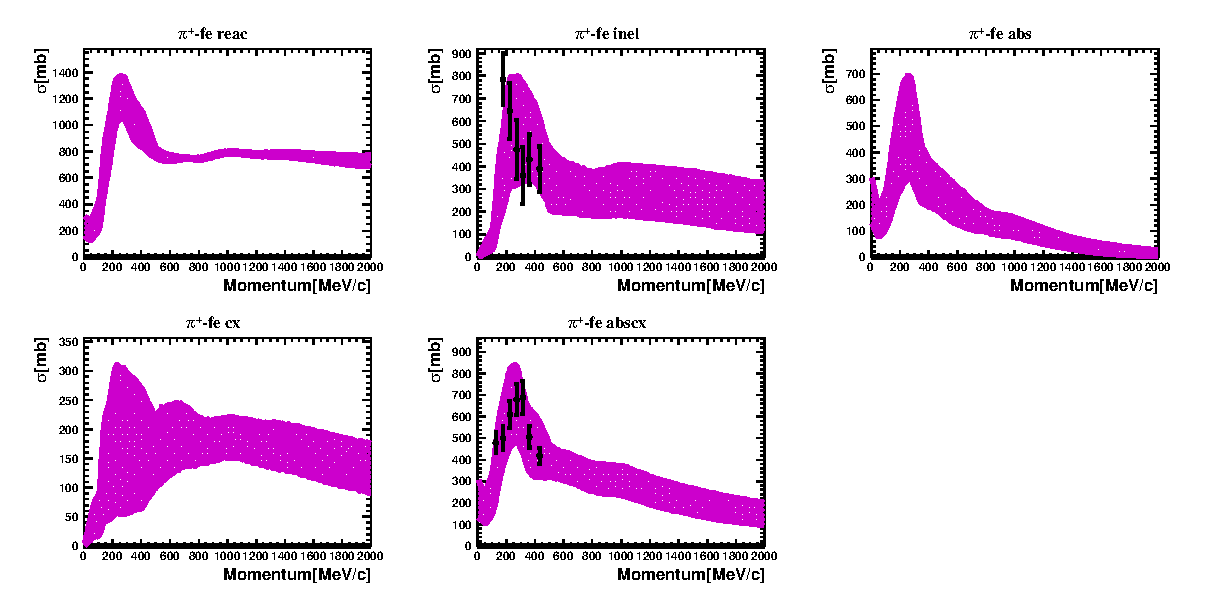
\includegraphics[width=0.9\textwidth]{T2K-TN-254/images/systematics/fe_piP_all.eps} 
  \caption[Comparison of pion scattering data to NEUT prediction and
  uncertainty]{Comparison of pion scattering data to \Gls{NEUT}
    prediction and uncertainty.  \textbf{\textit{Top five:}}
    Negatively charged pion on aluminium.  \textbf{\textit{Bottom
        five:}} Positively charged pion on iron.  From~\cite{FSITalk},
    for references, see in Table~(5.1) of~\cite{TN033}.}
  \label{fig:fsiheavy}
\end{figure}
\clearpage

\subsection{Effects on the selection}

The effects from the nucleon level pion production uncertainties are
shown in Figure~\ref{fig:infvpiproduncertainty}, which shows the
effects on the number of selected events for \Gls{FGD}1 \Gls{FV}
events only. Note that the \Gls{NC} coherent weight distribution shows
a spike at 45 events which corresponds to no coherent events in the
selection. Since the uncertainty is a Gaussian function centred at one
with an error of one; this is expected to happen 16\% of the time.

\begin{figure}[ht]
  \begin{adjustbox}{center}
    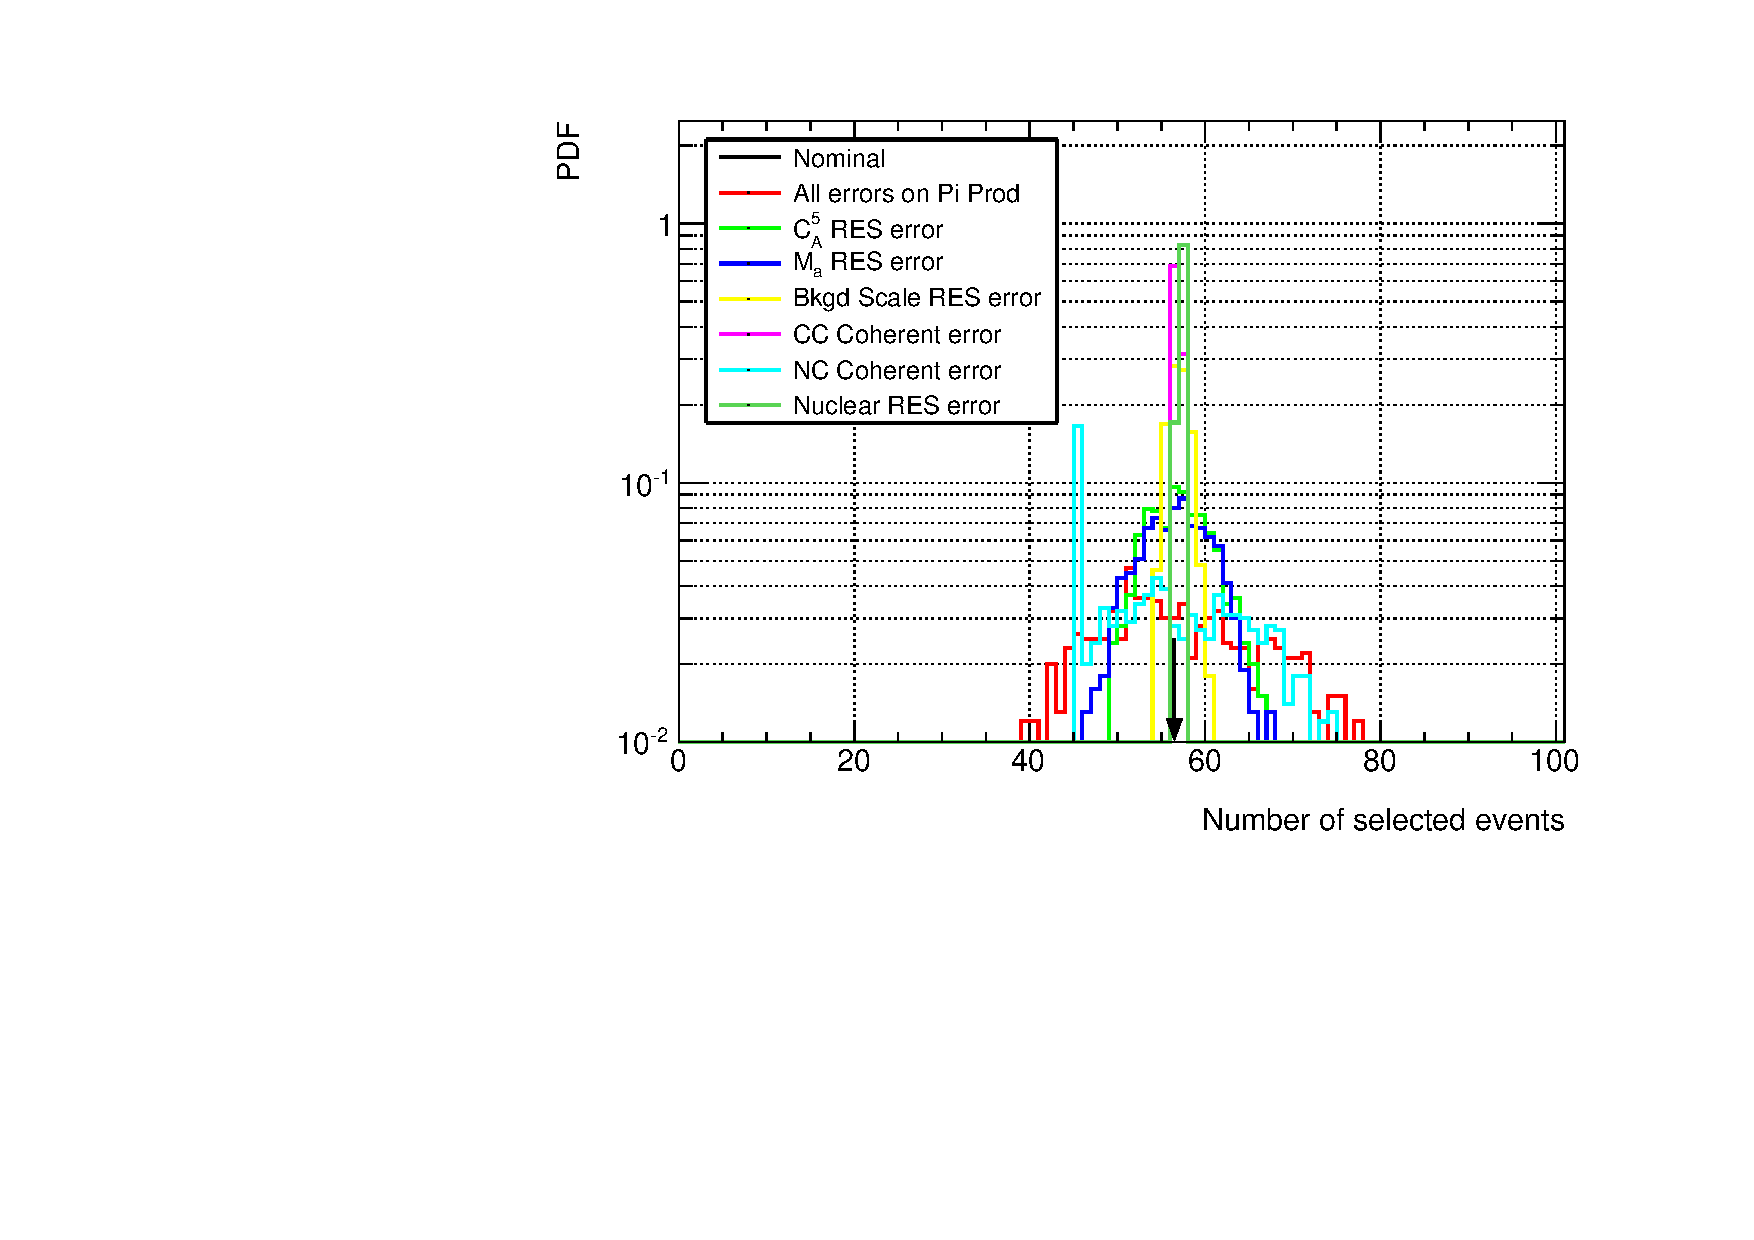
\includegraphics[width=0.8\textwidth]{images/NCg/PiProd.pdf} 
  \end{adjustbox}
  \center
  \caption[Effects of the pion resonant cross section uncertainties on
  the number of selected events]{Effects of the pion resonant cross
    section uncertainties on the number of selected events. The
    nominal central value is indicated by the black arrow.}
  \label{fig:infvpiproduncertainty}
\end{figure}

The other \Gls{CCQE} and \gls{nue} cross section errors effects are
shown in Figure~\ref{fig:infvotheruncertainty}.

\begin{figure}[ht]
  \center
  \includegraphics[width=0.8\textwidth]{images/NCg/Other_Jon.pdf} 
  \caption[Effects of the DIS (CC and NC), CCQE, CC coherent and nue
  cross section uncertainty on the number of selected events]{Effects
    of the \Gls{DIS} (\Gls{CC} and \Gls{NC}), \Gls{CCQE}, \Gls{CC}
    coherent and \gls{nue} cross section uncertainty on the number of
    selected events. The nominal central value is indicated by the
    arrow.}
  \label{fig:infvotheruncertainty}
\end{figure}


%%% Local Variables:
%%% mode: latex
%%% TeX-master: Thesis
%%% End:

\clearpage

\section{Detector systematic uncertainties}
\label{sec:detsyst}

The motivation for each of the detector uncertainty is detailed here.
There are three ways of implementing the \Gls{ND} detector systematic
uncertainties in \Gls{TK}, the first ones are called ``variation
systematics'', where the physical quantity (momentum and \Gls{TPC}
\Gls{PID} pull) that is being measured is changed according to the
effect of the systematic; another type controls the normalisation of a
whole class of events (so-called ``normalisation-like systematics'')
and finally, ``efficiency-like systematics'' which control, on an
event by event basis the weight of an event. All the uncertainties
that comes from detector effects are described here.

\subsection{Variation systematic uncertainties}

\subsubsection{The momentum scale uncertainty}
\label{subsec:momscale}
The magnetic field has an absolute error of $0.57\%$ that gets
directly propagated on the momentum of the particle~\cite{TN212}.

\subsubsection{The magnetic~/~electric field uncertainty}
\label{subsubsec:bfield}
The magnetic and electric field uncertainty~\cite{TN212} comes from
the fact that both the fields are not uniform in the \Gls{TPC}. This
is due to the presence of various equipment around the \Gls{TPC} or
the \Gls{TPC} case itself which produce fringe fields. In general, the
magnetic field and these fringe fields make the drift electrons from
the ionisation travel in a line which is not straight, which makes the
reconstruction more complicated. Some corrections can be applied at
the reconstruction level to take this effect into account, but there
is still a systematic uncertainty which has applied to the
reconstructed momentum.

On the cathode, some ``dots'' can be illuminated by lasers to produce
photo-electrons. These electrons drift until the readout plane, and
one can estimate the error on the corrections by calculating distance
from the reconstructed position of the dots to their real position.
This leads, at the analysis level, to an uncertainty on the momentum
of the particle.

\subsubsection{The momentum resolution uncertainty}
\label{subsec:momresol}
The \Gls{TPC} momentum resolution~\cite{TN212} was computed with
through going tracks that are reconstructed in multiple
\Glspl{TPC}. This systematic uncertainty aims at characterising the
intrinsic momentum resolution of the \Glspl{TPC}. The presence of
intermediate \Glspl{FGD} complicates the error calculation, as one
needs to correct for momentum loss in them. The uncertainty is
propagated on $1 / p_T$ where $p_T$ is the transverse momentum of the
particle (where transverse means orthogonal to the $Z$ direction, in
the $ZY$ plane). The uncertainty is around $10^{-4}$ for a
$500\text{~MeV}$ particle. This uncertainty is directly propagated on
the momentum of the particle.

\subsubsection{The \Gls{TPC} \Gls{PID} uncertainty}
\label{subsec:tpcpid}
The \Gls{PID} quantities that are used are the pulls, defined from the
$dEdx$ as shown in Equation~(\ref{eq:tpcpull}). To get an uncertainty
on these quantities, the pull is calculated for control samples on a
subset of the data available. This is then compared to the expected
\Gls{MC} distribution. In this case, the control sample is a photon
sample (electron~/~positron pairs with an invariant mass and good
\Gls{TPC} quality requirements). One obtains distributions similar to
the one shown in Figure~\ref{fig:tpcsyst} and can compare the width
and position of the Gaussian distributions which are used as
systematic uncertainties. In Figure~\ref{fig:tpcsyst}, on the right,
each of the data and \Gls{MC} distributions (in blue and green
histograms, respectively) are fitted with Gaussian functions (blue and
green curves). The \Gls{MC} predictions are then shifted to overlap
with the data by moving the mean of the Gaussian function for \Gls{MC}
and its spread, thus producing a correction that has to be applied to
the nominal \Gls{MC}.

The systematic uncertainty comes from the errors on the parameters of
the Gaussian functions, which is retrieved from the fit.

This is repeated for different momentum bin, particle type and, if the
statistics are sufficient, run period and \Gls{TPC} (in practice, this
split can only be realised for muons)~\cite{TN212}.

\begin{figure}[ht]
  \center
  \includegraphics[width=0.48\textwidth]{T2K-TN-254/images/corrections/nopidcor_lowMom.eps}
  \includegraphics[width=0.48\textwidth]{T2K-TN-254/images/corrections/pidcorr_lowMom_fit.pdf}
  \caption[PID pull for electrons (or positrons) of momentum smaller
  than $200$~MeV]{\textbf{\textit{Left:}} \Gls{PID} pull for electrons
    (or positrons) of momentum smaller than $200$~MeV.
    \textbf{\textit{Right:}} \Gls{PID} pull Gaussian fits for data
    (blue) and \Gls{MC} (green).}
  \label{fig:tpcsyst}
\end{figure}


\subsection{Efficiency systematic uncertainties}
The efficiency systematic errors are applied to the events and in
general are applied to both the pair and main tracks, unless stated
otherwise.

\subsubsection{The \Gls{TPC} cluster efficiency uncertainty}
\label{subsec:tpccluster}
The \Gls{TPC} cluster efficiency uncertainty~\cite{TN212} is applied
because there is a cut on the number of nodes the tracks creates in
the \Gls{TPC} (track quality cut). Note that clusters are horizontal
or vertical hits that are joined together (see the step~2 in the
\Gls{TPC} paragraph in Section~\ref{subsubsec:reconstruction}). This
was computed by comparing the number of nodes of muon data control
samples to its equivalent in the \Gls{MC}. These control samples are a
subset of a \Gls{CC} inclusive selection and cosmic muons
triggers. The selections are run without the \Gls{TPC} track quality
and the ratios
\begin{align}
  &\frac{\epsilon_\text{Data}}{\epsilon_\text{MC}} \label{eq:effcorrection}\\
  &\text{and~}\frac{\epsilon_{\text{MC}}-\epsilon_{\text{Data}}}{\epsilon_{\text{MC}}}\label{eq:efferror}
\end{align}
are computed (in these equations, $\epsilon$ indicate the data and
\Gls{MC} efficiency). It was then found that shifts one has to apply
to the \Gls{MC} (first ratio) and error (second ratio) are both the
order of one per mil.

\subsubsection{The \Gls{TPC} track efficiency uncertainty}
\label{subsubsec:tpctrack}
The \Gls{TPC} track efficiency uncertainty~\cite{TN212} characterises
the error one gets by solely requiring the presence of a track in the
\Gls{TPC}. Rather than cluster efficiency, this error is related to
the presence of a full reconstructed object as explained in the
\Gls{TPC} paragraph of Section~\ref{subsubsec:reconstruction} (step
3). The error is computed with through-going muons which cross several
detectors. The data and \Gls{MC} comparison for such sample show that
there is no unexpected behaviour in the all \Glspl{TPC} and that the
uncertainty does not depend on the momentum, position and number of
track crossing them. The error is around $0.5\%$ for a single track
entering the \Gls{TPC}2.

\subsubsection{The \Gls{TPC}~/~\Gls{FGD} matching efficiency uncertainty}
\label{subsubsec:tpcfgdmatch}
The \Gls{TPC}~/~\Gls{FGD} matching efficiency uncertainty~\cite{TN212}
arises because the tracks in the selection have to be reconstructed as
a single object. Note that, even though there is no explicit
requirement for the Pair Track to be in the \Gls{FGD} (only a distance
specification is made), there is a priori, no requirement to apply
this error for cases where the Pair Track does not use the
\Gls{FGD}. However this was considered to be a marginal effect that
happens only if the Main Track is next to the \Gls{TPC}, on the edge
of the \Gls{FGD}, so it was applied regardless of the topology of the
Pair Track.

The efficiency was computed using through-going muons crossing
different \Glspl{TPC}, and found to be exactly $100\%$ (i.e. no track
that enter the \Gls{TPC} from the \Gls{FGD} are missed, and vice
versa). Recalling that the \Gls{FGD}1 \Gls{FV} extends to the last
layer downstream, right next to the \Gls{TPC}2, and that only two bars
are removed in the upstream direction, this is maybe not
surprising. To assign the error, it was decided that the \Gls{TPC} /
\Gls{FGD} matching could fail if a track leaves only two hits in the
\Gls{FGD} (i.e. it is very close to its edge) and therefore the hit
efficiency is used as the error, which in this case is equal to about
$0.8\%$.

\subsubsection{The \Gls{TPC}~/~\Gls{ECal} matching efficiency uncertainty}
\label{subsubsec:tpcecalmatch}
It was found recently that the \Gls{ECal}'s representation in the
\Gls{MC} was few millimetres away from its real position. Therefore
there could be a mismatch between the probability in reconstructing a
particle in the \Gls{ECal} which came from the \Gls{TPC} in data and
\Gls{MC}. This could affect the \Gls{ECal} veto since there is a
requirement for the selected veto object to not be one of the two
tracks. An uncertainty is therefore applied on the \Gls{MT} of
\Gls{PT} when they enter the \Gls{ECal}. The uncertainty which is
propagated on these tracks is of the order of $5\%$~\cite{TN279}.

\subsubsection{Charge Identification uncertainty}
\label{subsubsec:chargeid}
The charge identification is a fundamental input to the analysis,
since it relies on the selection of two tracks of opposite charge.
The error that is used is determined from the control samples which
have a muon traversing several \Glspl{TPC}~\cite{TN212}. One can then
compare the probability to incorrectly swap the charge between data
and \Gls{MC}. The error decreases with the number of \Gls{TPC} the
particle traverses; in the worst case, when the track is reconstructed
in two \Glspl{TPC}, and each one reconstructs a different charge, the
uncertainty is of $2\%$.  The error is propagated on the inverse
transverse momentum as in the case of the momentum resolution.

\subsection{Normalisation uncertainties}
These uncertainties are applied to a whole class of events based on
their topologies, it generally does not rely on the detector
efficiencies themselves, but rather on other effects such as the cross
section (for the pion and proton secondary interaction), the mass
uncertainties (for the photon secondary interactions and the \Gls{FGD}
mass), or the presence of additional events (pile up uncertainties).

\subsubsection{\Gls{FGD} mass uncertainty}
\label{subsec:fgdmass}
The \Gls{FGD} has a mass uncertainty of $0.6\%$, which comes from the
uncertainty in size of its bars and the hole for the
fibre~\cite{TN212}.

\subsubsection{The pile up and sand uncertainties}
\label{subsec:pileup}
The pile up uncertainty comes from the fact that vetoes are present in
the selection. Indeed, additional ``\gls{sand}'' events that comes
from the sand around the \Gls{ND} can reach the detector and trigger
the veto of the selection. In the interest of time and space, these
events are not included in the standard ``\gls{magnet} \Gls{MC}''
(i.e. events that are in happening the volume enclosed by the \Gls{ND}
magnet) that is used for the analysis, they are added separately. The
problem is then, since these ``\gls{sand}'' events are added
separately on top of the simulation, how to see their effect on the
vetoes? For example, if a ``\gls{magnet}'' event is selected and
passes the selection, and if there was a ``\gls{sand}'' in the same
time, one would expect to select fewer events. Hence the name, the
magnet and sand events are ``piled up.''

The way to overcome this is by calculating a pile up correction and
uncertainty. For that, the strategy is to run a selection which only
has the vetoes, and comparing the data to the sum of the \gls{magnet}
\Gls{MC} and \gls{sand} \Gls{MC}. The vetoes are added in the same
order as in the selection.

Note that the \gls{sand} events have an intrinsic uncertainty of
$10\%$, which comes from the simulation of the surroundings of the
\Gls{ND}, the flux uncertainty and the cross section.

Upon assigning the pile up correction, the strategy is to modify the
normalisation of the whole selection based on the \gls{sand} trigger
rate one gets. The error is either the data~/~\Gls{MC} difference, or
the \gls{sand} error if it is greater than the former. All the errors
and corrections are listed in Table~\ref{tab:pileup}, note that the
correction is dependent on the run, since the \Gls{MR} power increases
and produces different yields in the vetoes due to the expected
increase in \gls{sand} interaction and thus pile up.

\begin{table}[ht]
  \center
  \begin{tabular}{cccc}
    \toprule
    Veto & Run & Correction & Systematic uncertainty \\
    \cmidrule(r){1-4}
    \multirow{6}{*}{\Gls{TPC} muon rejection} & 2A  & 0.992 & 0.009 \\
         & 2W  & 0.993 & 0.007 \\
         & 3AB & 0.994 & 0.009 \\
         & 3AC & 0.991 & 0.009 \\
         & 4A  & 0.989 & 0.010 \\
         & 4W  & 0.990 & 0.010 \\
    \cmidrule(r){1-4}                        
    \multirow{6}{*}{\Gls{TPC} Veto} & 2A  & 0.995 & 0.008 \\
         & 2W  & 0.996 & 0.007 \\
         & 3AB & 0.996 & 0.008 \\
         & 3AC & 0.994 & 0.009 \\
         & 4A  & 0.992 & 0.010 \\
         & 4W  & 0.994 & 0.010 \\
    \cmidrule(r){1-4}                        
    \multirow{6}{*}{\Gls{PD} Veto} & 2A  & 0.928 & 0.009 \\
         & 2W  & 0.936 & 0.008 \\
         & 3AB & 0.937 & 0.009 \\
         & 3AC & 0.920 & 0.010 \\
         & 4A  & 0.897 & 0.012 \\
         & 4W  & 0.906 & 0.010 \\
    \cmidrule(r){1-4}
    \multirow{6}{*}{\Gls{ECal} Veto} & 2A  & 0.9989 & 0.0006 \\
         & 2W  & 0.9983 & 0.0007 \\
         & 3AB & 0.9991 & 0.0007 \\
         & 3AC & 0.9979 & 0.0008 \\
         & 4A  & 0.9974 & 0.0008 \\
         & 4W  & 0.9967 & 0.0010 \\

    \bottomrule
  \end{tabular}
  \caption[Pile up corrections and systematic uncertainties used in
  the analysis]{Pile up corrections and systematic uncertainties used
    in the analysis.}
  \label{tab:pileup}
\end{table}

Finally, as no \gls{sand} event enters the actual selection, they thus
lead to no additional uncertainty.

\subsubsection{The pion secondary interaction uncertainty}
\label{subsec:pionsec}
The pion secondary interaction uncertainty~\cite{TN212} is a weight
error that is propagated on the events which have charged pions in
them. A secondary interaction happens when this pion reinteracts with
some of the detector material, rather than losing energy by ionisation
in the detector.

There are a lot of channels in which a charged pion can interact, but
the most important in the context of this analysis is the charge
exchange channel, where a pion goes from being a charged pion to a
neutral pion after interaction with a nucleus. Unfortunately, the
\Gls{MC} model that was implemented in the \Gls{ND} simulations
(Bertini model~\cite{WRIGHT2015175}) was found to very poorly describe
the available data at \Gls{TK}
energies~\cite{TN125,TN325,Ashery:1981tq} ($200\text{~MeV}$);
therefore a correction factor was included in the cross section for
charged pions. The error on the above mentioned
data~\cite{Ashery:1981tq} was also propagated to the weight to be able
to get an uncertainty on the secondary pion interaction. Note that
these are completely uncorrelated with the \Gls{FSI} errors as
described earlier; correlating the pion secondary interaction and the
\Gls{FSI} will constitute an improvement for the next generation of
analyses at the \Gls{ND}.

\subsubsection{The proton secondary interaction uncertainty}
\label{subsec:protonsec}
The proton secondary interaction probability uncertainty~\cite{TN212}
is propagated if the \Gls{MT} or \Gls{PT} is a proton. This happens if
the \Gls{PID} did not work properly, for example. The low energy
protons have a probability of interacting with the scintillator in the
\Gls{FGD} and can reinteract in it. A very conservative error of
$10\%$ is applied for the proton interactions.

\subsubsection{The photon secondary interaction uncertainty}
\label{subsec:photonsec}
\input{T2K-TN-313/systematicsoofv.tex}

\subsubsection{Out of fiducial volume reconstruction uncertainty}
\label{subsec:recooofv}
This uncertainty is propagated because the \Gls{MT} and \Gls{PT} are
selected inside the \Gls{FV} of the detector. This was based on work
from~\cite{TN098}. It can happen that the tracks come from outside the
fiducial volume but are reconstructed inside if for example there was
a failure to detect a hit in the outer layers of the \Gls{FGD}, or a
hard scatter in the \Gls{FGD} that somehow confuses the
reconstruction. These can sometime have a large uncertainty ($30$ to
$50\%$) depending on the topology of the track.


\subsection{Summary of the detector uncertainties}
\label{subsec:detsystsummary}

Table~\ref{tab:detectoruncertaintyinfv} gives a summary of the overall
effects of all the detector errors. Note that in this table, the
positive and negative errors are determined using the \Gls{HPD}
(Highest Posterior Density) method\footnote{The following method was
  used to calculate the error of a distribution:
  \begin{itemize}[noitemsep,topsep=0pt]
  \item Find the mode of the distribution, which is now referred as
    $N_\text{event}^\text{mode}$,
  \item Create an interval for which the \Gls{PDF} is constant and
    contain the $68\%$ of the total distribution,
  \item Read off the values corresponding to the number of events (on
    the X axis) the positive and negative values are called
    $N_\text{event}^{\pm}$,
  \item Use the values
    $\frac{\left|N_\text{event}^\text{mode} -
        N_\text{event}^\pm\right|}{N_\text{event}^\text{mode}}$ as the
    positive and negative relative uncertainties. \label{ftn:hpd}
  \end{itemize}
}. Note that this method is quite sensitive to the number of toy
thrown and the binning chosen for the computation.

Figure~\ref{fig:detectorsystematicsinfv} shows the \Gls{PDF} of the
selected event after propagation of the detector errors.

\begin{table}[ht]
  \center
  \begin{tabular}{ll}
    \toprule
    Systematic & Relative uncertainty \\
    \midrule
    \multicolumn{2}{l}{Weight errors} \\
    \midrule
    Charge identification efficiency         & 0.002  \\
    \Gls{TPC} cluster efficiency             & 0.000009\\
    \Gls{TPC} track efficiency               & 0.011  \\
    \Gls{TPC}~/~\Gls{FGD} matching efficiency& 0.006  \\
    \Gls{TPC}~/~\Gls{ECal} matching efficiency & $< 0.00001$  \\
    \Gls{FGD} mass                           & 0.043  \\
    Secondary interaction pion               & 0.046  \\
    Secondary interaction proton             & 0.026  \\
    Secondary interaction photon             & $\pm^{0.41}_{0.15}$  \\
    Reconstructed \Gls{OOFV}                 & 0.061  \\
    \Gls{ECal} pile up                       & 0.0004 \\
    Muon rejection pile up                   & 0.0004  \\
    \Gls{PD} pile up                         & 0.006  \\
    \Gls{TPC} pile up                        & 0.005  \\
    \midrule
    \multicolumn{2}{l}{Variation errors} \\
    \midrule
    Magnetic field      & 0.009 \\
    Momentum scale      & 0.022 \\
    Momentum resolution & 0.025 \\
    \Gls{TPC} \Gls{PID} & 0.019 \\
    \midrule
    Total & $\pm^{1.24}_{0.20}$ \\
    \bottomrule
  \end{tabular}
  \caption[Detector uncertainties for the selected events]{Relative
    detector uncertainties for the events that pass the selection.}
  \label{tab:detectoruncertaintyinfv}
\end{table}

\begin{figure}[ht]
  \center
  \includegraphics[width=0.8\textwidth]{images/NCg/Det.pdf} 
  \caption[Effect of the detector uncertainty on the number of
  selected events]{Effect of the detector uncertainty on the number of
    selected events. The nominal central value is indicated by the
    arrow.}
  \label{fig:detectorsystematicsinfv}
\end{figure}


%%% Local Variables:
%%% mode: latex
%%% TeX-master: "Thesis"
%%% End:

\clearpage

\section{Total uncertainty}
\label{sec:totaluncertainty}


\subsection{Statistical uncertainty}
\label{subsec:statuncertainty}
To account for statistical uncertainty, the data normalisation was
thrown according to a Poisson distribution of parameter the number
events expected. Similarly, for the \Gls{MC} statistic uncertainty,
same procedure was applied without any weight nor correction or
tuning. Doing this, one finds that the relative statistical
uncertainty is \datastaterror for the data, and \mcstaterror for the
\Gls{MC}. The effect on the selected events is shown in
Figure~\ref{fig:statuncertainty}.

\begin{figure}[ht]
  \begin{adjustbox}{center}
    \includegraphics[width=0.8\textwidth]{images/NCg/stat.pdf}
  \end{adjustbox}
  \caption[Effect of all the statistical uncertainties on the number
  of selected events]{Effect of all the statistical uncertainties
    (data and \Gls{MC}) on the number of selected events. The nominal
    central value is indicated by the arrow.}
  \label{fig:statuncertainty}
\end{figure}

\subsection{Efficiency uncertainty}
\label{subsec:effuncertainty}
The efficiency also has an systematic error associated to it. To get
it, the statistical uncertainty on the number of events selected after
all the cuts is computed (simply the square root of the number of
event divided by the number of event selected).  To do this, a very
high \Gls{POT} of \Gls{NCg} events have been generated
($6.5\times 10^{24}$ \Gls{POT}).

\subsection{Combination of asymmetric error}
\label{subsec:combinationerror}
To combine all the systematic errors and get a toy distribution
allowing a proper treatment of the very asymmetric detector error that
was discussed in the previous sections, a ``discrete convolution
method'' was proposed, this method is now described.

All the independent errors were thrown, including the Poisson
statistical uncertainty of the data and MC. In a standard cross
section analysis where all the errors that are Gaussian, the errors
are then added in quadrature and get the number of event at 90\%
\Gls{CL}, $N_\text{events}^{90\%CL}$, by integrating:
\begin{equation}
\label{eq:integral}
0.90 = \int^{N_\text{events}^{90\%\text{CL}}}_{-\infty}\text{Gauss}\left(\mu = N_\text{events}^\text{nominal}, \sigma \right) dN_\text{events},
\end{equation}
where $N_\text{events}^\text{nominal}$ is the nominal number of events
after all the correction and tuning, and $\sigma$ is the total
uncertainty on this number after summing all the independent errors in
quadrature.

Note that the assumption that one can add the errors in quadrature is
central in this method. However, it cannot be applied for asymmetric
errors as is the case in this analysis.

Rather than adding the errors in quadrature, the ratios
$N_\text{events}^\text{toy} / N_\text{event}^\text{nominal}$ were
computed for each toy and for each uncertainty source. To get the
total \Gls{PDF} (Probability Distribution Function) of the number of
selected events, one just has to multiply all these ratios with each
other:
\begin{equation}
\label{eq:toycombination}
N_\text{events}^\text{toy} = N_\text{event}^\text{nominal} \times \prod_{i = \text{source}}\prod_{j = \text{toy}}
\frac{N_\text{events}^{\text{toy} i,j}}{N_\text{events}^\text{nominal}},
\end{equation}
where $i$ denotes the source of the uncertainty (it can be detector,
flux, \Gls{FSI}, cross section, data or \Gls{MC} statistics), and $j$
is the particular toy. In practice, the number of toy experiments
grows exponentially with the number of source of systematic errors,
therefore the systematic uncertainties with Gaussian behaviour (flux,
cross section, \Gls{FSI}, data and \Gls{MC} statistics) were added in
quadrature and used to generate 1000 toy experiments to combine with
the asymmetric detector uncertainty as described earlier.

\subsection{Effect of all uncertainties}
When combining the uncertainties as described in the previous section,
one obtains the distribution shown in Figure~\ref{fig:allsyst}.

\begin{figure}[ht]
  \begin{adjustbox}{center}
    \includegraphics[width=0.8\textwidth]{images/NCg/All.pdf}
  \end{adjustbox}
  \caption{Effect of all the uncertainties in the total number of
    selected events.}
  \label{fig:allsyst}
\end{figure}

Note, that as can be seen in Figure~\ref{fig:detectorsystematicsinfv},
the detector systematic uncertainties introduce a relatively large
bias towards higher number of events. This bias gets propagated on the
total systematic uncertainty distribution (``All errors'' on
Figure~\ref{fig:allsyst}), but not on the other distributions (cross
section errors, \Gls{FSI}, flux). This is why the error on pion
production \Gls{PDF} seems to extend towards lower number of events
than the one with all the errors. It was checked that appling the same
bias to the pion production error gives shifts the pion production
error \Gls{PDF} under the one with all the errors.

\subsection{\texorpdfstring{Motivation of the $\varphi_\text{photon}$ cut}%
  {Motivation of the photon phi cut}}
\label{subsec:downwardphotons}

An interesting feature is exhibited in Appendix~\ref{app:mass}, for
bottom-originated events, there is a higher uncertainty than for the
rest of the selection (Table~\ref{tab:oofvmasserror}). Since the
pointing capabilities of the \Gls{FGD}1 is reasonably good for event
coming from all the directions (see Appendix~\ref{app:rec}), one can
restrict the phase space to events originated from the top and the
side directions. This is done with a simple cut on the $\varphi$ angle
of the reconstructed photon direction.  The effect of adding this
phase space cut is shown in Figure~\ref{fig:detectorphi}.

However, such a cut would have an impact too drastic on the efficiency
and on the statistics of the selected events. So, rather than removing
all the events from the downward direction, the cut was optimised. To
do that, the only uncertainties of interest are the detector
systematic errors and the data statistical error. Similarly, the
efficiency is going to decrease if one removes too many events from
downward. The optimisation of this cut was performed by minimising its
value by minimizing the value $N_\text{Signal}/\epsilon$

In this ratio, $N_\text{Signal}$ is the difference between the 90\%
upper \Gls{CL} of the number of \Gls{MC} events and the nominal number
of events (which essentially gives an idea of the uncertainty) and
$\epsilon$ is the efficiency. The Figure~\ref{fig:optimisationphi}
motivates the chosen value of $\varphi_\text{cut} = 36^{\circ}$. This
value is then translated for the excluded angles
$\varphi_{\text{photon}}$:

\begin{align}
  -90^{\circ} - \varphi_{\text{cut}} / 2 &< \varphi_{\text{photon}} < -90^{\circ} + \varphi_{\text{cut}} / 2 \\
  -108^{\circ} & <  \varphi_{\text{photon}} < -72^{\circ}.
\end{align}

All the errors are depicted in Figure~\ref{fig:allsystphi} and
summarised in Table~\ref{tab:AllErrorPhiCut} after this cut (called
$\varphi_\text{photon}$ cut from now on). Note that in this table, the
positive and negative errors are determined using the \Gls{HPD}
(Highest Posterior Density) method (see Footnote~\ref{ftn:hpd} on
page~\pageref{ftn:hpd}). As explained earlier, this method is quite
sensitive to the number of toy thrown and the binning chosen for the
computation. For example, it fails in giving a reasonable answer for
the \Gls{COH} cross section error, since the highest probability is at
the edge of its \Gls{PDF}. Therefore, only the detector and the total
errors have been computed using this method.

\begin{figure}[ht]
  \begin{adjustbox}{center}
    \includegraphics[width=0.8\textwidth]{T2K-TN-254/images/systematics/QuantilePhiBTZ.pdf} 
  \end{adjustbox}
  \caption[PDF of the selected number of events from the detector
  uncertainties after the azimuthal cut ($\varphi > 0$)]{\Gls{PDF} of
    the selected number of events from detector uncertainties
    (including the \Gls{OOFV} one) after the azimuthal cut
    ($\varphi > 0$). The nominal central value is indicated by the
    arrow.}
  \label{fig:detectorphi}
\end{figure}

\begin{figure}[ht]
  \begin{adjustbox}{center}
    \includegraphics[width=0.8\textwidth]{T2K-TN-254/images/systematics/Optimisation.pdf} 
  \end{adjustbox}
  \caption[Optimisation of the $\varphi$ cut]{Optimisation of the
    $\varphi$ cut, showing the contribution of the data statistic,
    detector systematic errors and efficiency on
    $N_\text{Signal}/\epsilon$, which is proportional to the cross
    section limit.}
  \label{fig:optimisationphi}
\end{figure}

\begin{figure}[ht]
  \begin{adjustbox}{center}
    \includegraphics[width=0.8\textwidth]{T2K-TN-254/images/systematics/QuantilePhi.pdf} 
  \end{adjustbox}
  \caption[PDF of the selected number of events from the detector
  uncertainties after the optimised azimuthal cut (with events
  satisfying $-108^{\circ} < \varphi_{\text{photon}} < -72^{\circ}$
  excluded)]{\Gls{PDF} of the selected number of events from the
    detector uncertainties after the optimised azimuthal cut (with
    events satisfying
    $-108^{\circ} < \varphi_{\text{photon}} < -72^{\circ}$ excluded).
    The nominal central value is indicated by the arrow. The $90\%$
    quantile of the \Gls{MC} is also shown.}
  \label{fig:allsystphi}
\end{figure}

\begin{table}[ht]
  \begin{adjustbox}{center}
    \begin{tabular}{lc}
      \toprule
      Systematic error &Relative uncertainty \\ 
      \midrule
      Statistical error on Data (expected) & $\pm 0.14$ \\ 
      Statistical error on Data (observed) & $\pm 0.16$ \\ 
      Statistical error on \Gls{MC}        & $\pm 0.032$ \\ 
      \midrule
      Detector errors                      & $\pm^{0.27}_{0.17}$\\ 
      \midrule
      $C_{A}^{5}$ \Gls{RES} error              &$\pm0.078$ \\ 
      $M_{a}$ \Gls{RES} error                 &$\pm0.089$ \\ 
      Background scale \Gls{RES} error        &$\pm0.023$\\ 
      Nuclear \Gls{RES} ($\Delta$ mass) error &$\pm0.002$\\ 
      \midrule                                
      All errors on single pion production    &$\pm0.20$\\ 
      \midrule
      \Gls{CCQE} errors        & $\pm 0.003 $\\ 
      \Gls{CC}\Gls{nue} error  & $\pm 0.006 $\\ 
      \Gls{DIS} error          & $\pm 0.012 $\\ 
      \Gls{CC} \Gls{COH} error & $\pm 0.001 $\\ 
      \Gls{NC} \Gls{COH} error & $\pm 0.163 $\\ 
      Other \Gls{NC} error     & $\pm 0.032 $\\ 
      \midrule
      All cross section errors (except single pion production) & $\pm 0.036$\\ 
      \midrule
      Flux error & $\pm 0.082$\\ 
      \midrule
      \Gls{FSI} error & $\pm 0.037$\\
      \midrule
      Efficiency error & $\pm 0.0985$ \\
      \midrule
      All errors (except efficiency) & $\pm^{0.33}_{0.23}$ \\ 
      \bottomrule
    \end{tabular}
  \end{adjustbox}
  \caption[Summary of all the errors after the $\varphi$ angle
  cut]{Summary of all the errors after the $\varphi$ angle cut using
    the \Gls{HPD} method.}
  \label{tab:AllErrorPhiCut}
\end{table}


\subsection{Conclusion}
In this section, the importance of each systematic uncertainty and its
effect on the number of selected events were shown. In the case of a
analysis which aims to set a limit, careful characterisation of the
systematic uncertainties is primoridial. This is because the limit is
directly proportional to the total systematic errors (at least in the
case of Gaussian errors). All the asymmetric errors were added
coherently via the described method of discrete convolution. The main,
dominant, error is the detector uncertainty. This error is mitigated
by adding a cut on the reconstructed azimuthal angle of the photon and
removing the photons that comes from under the \Gls{ND}, which have a
large propagation error.

%%% Local Variables:
%%% mode: latex
%%% TeX-master: "Thesis"
%%% End:

\clearpage


%%% Local Variables:
%%% mode: latex
%%% TeX-master: "Thesis"
%%% End:

\clearpage

\chapter{Results}
\label{chap:result}
\section{Monte Carlo sensitivity}
\input{T2K-TN-254/extraction.tex}
\section{Data result}
\input{T2K-TN-254/data.tex}
\section{Discussion}
\input{T2K-TN-254/conclusion.tex}

\clearpage
\newpage
\blankpage

\chapter{Fitting the ND280 samples to constrain oscillation analysis
  systematic errors with electron samples}
\label{chap:banff}



\section{Introduction}
\label{sec:banffintroduction}

In this section, the \Gls{ND} inclusive electron (anti-) neutrino
samples and the \Gls{ND} muon (anti-) neutrino samples in \Gls{RHC}
are used in the context of oscillation analysis. This was never
realised previously on \Gls{TK}. This study has three goals, two of
which are related to the electron (anti-) neutrino appearance samples
at \Gls{SK} in light of the search for \Gls{CP} violation in the
neutrino sector. The other goal is related to the muon (anti-)
neutrino disappearance measurement at \Gls{TK}. These goals are:
\begin{itemize}[noitemsep,topsep=0pt]
\item The consolidation of the result for \Gls{CP} violation by moving
  from a theory-driven electron neutrinos cross section uncertainty to
  an equivalent data-driven uncertainty.
\item An overall the reduction of systematic uncertainties related to
  the electron (anti-) neutrinos appearance samples at \Gls{SK}: as
  will be shown in this chapter, the data result can be improved
  simply by collecting more data, as opposed to the theory-driven
  error.
\item Finally, this study can be used for testing the single pion
  model in the anti-neutrino sector. This has some importance in the
  oscillation in the atmospheric sector using the anti-neutrino
  disappearance samples.
\end{itemize}

In the second section, the oscillation analysis strategy is
explained. Then, the framework for characterising the oscillation
analyses systematic uncertainties with the \Gls{ND} is described, and
the samples used in the fit are described. In the subsequent sections,
the expected sensitivity and the data result are shown. Finally, the
propagation of the sensitivity to the \Gls{CP} violation allowed
region is shown.


\section{The TK oscillation analysis strategy}
\label{sec:oscillationanalysis}
In this section, the strategy for the oscillation analyses in \Gls{TK}
is explained. There are three main analyses on \Gls{TK} that produce
the oscillation parameter results. Two of them use a semi-frequentist
approach and aim to produce confidence intervals on oscillation
parameters, and run a fit over them and the nuisance parameters.
These two analyses are called ``\gls{p-theta}'' and
``\Gls{VALOR}''~\cite{VALOR}, both of them use a
Minuit2~\cite{James:1975dr} log-likelihood fit. The other one uses a
Markov-Chain Monte Carlo (\Gls{MCMC}) to sample over the parameter
space; it is called ``\Gls{MaCh3}''~\cite{MACH3}. It is a fully
Bayesian analysis and produces credible intervals on neutrino mixing
parameters.

The fact that the oscillation analyses are repeated by different
groups allows validation and comparisons of the result.

These analyses use the multiple inputs from different \Gls{TK}
groups. The inputs are listed here:
\begin{itemize}
\item The beam group provides the absolute flux histograms (such as
  the one shown in Figure~\ref{fig:flux1}), the flux covariance matrix
  which encloses all the systematic errors on these histograms (see
  Figure~\ref{fig:flux2} and Section~\ref{sec:fluxsyst}) and the flux
  tuning which is, as described in Section~\ref{fig:beamline},
  determined from {\it in situ} measurements of the beam and
  additional hadron production data from
  NA61~/~SHINE~\cite{Abgrall:2011ae,Abgrall:2011ts,Abgrall:2015hmv}.
\item The neutrino interaction working group (\Gls{NIWG}) provides a
  parametrisation for the cross section and ``prefit'' systematic
  errors on each of the nuisance parameter of interest. These
  generally rely on the use of external data sets and fit such as the
  one described in~\cite{CallumFit}, discussions with theorists, and
  phenomenology work done within \Gls{TK}.
\item The \Gls{ND} data, which is used before the main oscillation fit
  to constrain the flux and cross section systematic
  uncertainties. Traditionally, the \Gls{ND} data that was used for
  the fits was restricted to the \Gls{numu} and \Gls{anumu} data,
  however the aim of this analysis is to include samples sensitive to
  the background \Gls{nue} flux (which represent around $1\%$ of the
  neutrino at the flux peak) to constrain cross section and flux
  parameters. Fitting these parameters with such samples can introduce
  anti-correlation between flux and cross section parameters (i.e. at
  constant number of \Gls{nue} in the \Gls{ND}, if the flux increases,
  the cross section has to decrease).
\item The \Gls{SK} \Gls{CCQE}-like \gls{numu}, \gls{nue}, \gls{anumu}
  and \gls{anumu} samples, and the \Gls{nue} \Gls{CC}$1\pi^+$ sample.
\end{itemize}

Note that the statistical power of the data from the \Gls{ND} is much
larger than the one from \Gls{SK}. This means that \Gls{ND} data
uncertainty is largely dominated by systematic uncertainties, whereas
the \Gls{SK} data uncertainty is mostly statistical (especially for
the appearance samples, the \gls{nue} and \gls{anue} samples),
although this is becoming less and less true as \Gls{TK} data is being
collected.

For all the three oscillation analyses, the first step is to fit the
\Gls{ND} data to constrain flux and cross section parameters. Once an
acceptable fit ($p_\text{value} > 5\%$) is reached, it is considered
that the parametrisation is sufficient for an oscillation fit and the
errors are propagated to \Gls{SK}.

There are other mechanisms to check that the parametrisation is
sufficient under significant change of cross section model, called
fake data, but these are beyond the scope of the analysis that is
presented here.

In this section, the focus is on the \Gls{ND} fits that are used in
oscillation analyses. This step is essential to reduce the systematic
uncertainties on the cross section and neutrino flux.


\section{Beam and Near Detector Fit Framework}
\label{sec:BANFF}
The software framework used for this is called \Gls{BANFF}. It
performs a Minuit2~\cite{James:1975dr} fit and minimises the Poisson
logarithmic likelihood with extra $\chi^2$ penalty terms for the
systematic error. They are defined as follows:

\begin{align}
  \label{eq:likelihood}
  -2\ln(\mathcal{L}) &= 2 \sum_{i=0}^{\text{N bins}}N^{p}_{i}(\vec{b},\vec{x},\vec{d})-N^{d}_{i}
                       +N^{d}_{i}\ln[N^{d}_{i}/N^{p}_{i}(\vec{b},\vec{x},\vec{d})] \\
                     &+\sum_{k,l=0}^{E_{\nu}\text{~bins}}\Delta b_{k}(V^{-1}_\text{beam})_{k,l}\Delta b_{l} \nonumber \\
                     &+\sum_{m,n=0}^{\text{xsec param}}\Delta x_{m}(V^{-1}_\text{xsec})_{m,n}\Delta x_{n} \nonumber \\
                     &+\sum_{i,j=0}^{\text{N bins}}\Delta d_{i}(V^{-1}_{\text{det}})_{i,j}\Delta d_{j},\nonumber 
\end{align}
where $\mathcal{L}$ is the total likelihood (note that
$-2\ln(\mathcal{L})$ can be approximated to a $\chi^2$ function for
sufficient statistics), $i$ and $j$ are the bin numbers for the
reconstructed quantities $p_\text{lepton}$ (momentum of the leading
lepton) and $\cos(\theta_\text{lepton})$ (cosine of the angle between
the neutrino direction and the leading
lepton). $N^{p}_{i}(\vec{b},\vec{x},\vec{d})$ is the number of
expected events in the $i^{\text{th}}$ bin, which depends on
$\vec{b}$, the beam weight, which encloses the action of the flux
systematic uncertainties on the events; $\vec{x}$, the cross section
weight, which parametrises the effect of the cross section systematic
uncertainties and $\vec{d}$, the detector weight, which parametrises
the detector uncertainty in each reconstructed bin. $N^d_i$ is the
number of events seen in the $i^{\text{th}}$ bin.

$V_\text{beam}$, $V_\text{xsec}$ and $V_\text{det}$ represent the
covariance matrices of the flux, cross section and detector systematic
uncertainties, respectively. They respectively correlate: the number
of neutrinos in each true energy bin in the case of the flux, the
cross section parameters, and the number of events in each
reconstructed bin. $\Delta b$, $\Delta x$, $\Delta d$, are the
variations of the beam, cross section and detector parameters with
respect to their nominal values, respectively.

\section{Samples used}
\label{sec:samples}
The samples that are used are \Gls{ND} ``tracker'' samples (i.e. they
do not include the analyses where the \Gls{PD} is used as a
target). These analyses are divided according to their topology,
detector (\Gls{FGD} 1 or 2) and whether the neutrino beam is running
in neutrino mode (\Gls{FHC}) or anti-neutrino mode
(\Gls{RHC}). Twenty-eight binned samples are used in the fit. The
first six samples have not changed compared to previous analyses:
\begin{itemize}[noitemsep,topsep=0pt]
\item 3 \Gls{numu} \Gls{CC} selections in \Gls{FGD}1 in \Gls{FHC}: 1
  muon + 0 pion; 1 muon + 1 positively charged pion; 1 muon +
  everything else;
\item 3 \Gls{numu} \Gls{CC} selections in \Gls{FGD}2 in \Gls{FHC}: 1
  muon + 0 pion; 1 muon + 1 positively charged pion; 1 muon +
  everything else.
\end{itemize}
The remaining samples are new selections that have been used for the
first time in this fit:
\begin{itemize}[noitemsep,topsep=0pt]
\item 3 \Gls{anumu} \Gls{CC} selections in \Gls{FGD}1 in \Gls{RHC}: 1
  anti-muon + 0 pion; 1 anti-muon + 1 negatively charged pion; 1
  anti-muon + everything else;
\item 3 \Gls{anumu} \Gls{CC} selections in \Gls{FGD}2 in \Gls{RHC}: 1
  anti-muon + 0 pion; 1 anti-muon + 1 negatively charged pion; 1
  anti-muon + everything else;
\item 3 \Gls{numu} \Gls{CC} selections in \Gls{FGD}1 in \Gls{RHC}: 1
  muon + 0 pion; 1 muon + 1 positively charged pion; 1 muon +
  everything else;
\item 3 \Gls{numu} \Gls{CC} selections in \Gls{FGD}2 in \Gls{RHC}: 1
  muon + 0 pion; 1 muon + 1 positively charged pion; 1 muon +
  everything else;
\item Inclusive \Gls{nue} \Gls{CC} selection in \Gls{FGD}1 in
  \Gls{FHC};
\item Inclusive \Gls{nue} \Gls{CC} selection in \Gls{FGD}2 in
  \Gls{FHC};
\item Inclusive \Gls{anue} \Gls{CC} selection in \Gls{FGD}1 in
  \Gls{RHC};
\item Inclusive \Gls{anue} \Gls{CC} selection in \Gls{FGD}2 in
  \Gls{RHC};
\item Inclusive \Gls{nue} \Gls{CC} selection in \Gls{FGD}1 in
  \Gls{RHC};
\item Inclusive \Gls{nue} \Gls{CC} selection in \Gls{FGD}2 in
  \Gls{RHC};
\item Photon sample in \Gls{FGD}1 selection in \Gls{FHC};
\item Photon sample in \Gls{FGD}2 selection in \Gls{FHC};
\item Photon sample in \Gls{FGD}1 selection in \Gls{RHC};
\item Photon sample in \Gls{FGD}2 selection in \Gls{RHC}.
\end{itemize}

For previous iterations of these fits~\cite{TN324}, the \Gls{RHC} were
using a different categorisation, and had a split between \Gls{numu}
\Gls{CC} with one or several tracks (so-called ``\Gls{CC} 1-track''
and ``\Gls{CC} n-tracks''). The electron samples had never been used
in the these fits. However, they are used in \Gls{NOvA}
analyses~\cite{PhysRevLett.118.231801}).

The remainder of this section covers the description of the samples
used and how they are selected. Firstly, the amount of \Gls{POT} that
is used is shown. Then, the selections are broadly described. The
binning used is detailed in Appendix~\ref{app:binning}.

\subsection{Run periods and Proton On Target}
\label{subsec:pot}
The data sets used correspond to the data collected with the \Gls{ND}
when all the sub-detectors are in place (excluding run~1), up to
summer 2017, all the corresponding \Gls{POT} is listed in
Table~\ref{tab:POTBANFF}. Note that the year 2017 data was only
partially calibrated (so called ``\gls{pc1}''), which is different
from all the rest of the data which was fully calibrated
(``\gls{rdp},'' for real data processing). The \Gls{ECal} run~8 data
was not fully calibrated at the time this document was written. This
has an impact on the \Gls{nue} selections which are using the
\Gls{ECal} for \Gls{PID}, as will be explained in the next section, so
the run~8 data was not used for the electron neutrino
selections. However, this has no impact on the muon neutrinos
selections, so this data was used for these selections.

\begin{table}[ht]
  \begin{adjustbox}{center}
    \begin{tabular}{llllll}
      \toprule
      \multirow{2}{*}{Runs} & \multicolumn{5}{c}{POT}\\
                            & Data & \multicolumn{2}{l}{\Gls{magnet} \Gls{MC} (ratio)} & \multicolumn{2}{l}{\Gls{sand} \Gls{MC} (ratio)} \\
      \midrule
      2a  (\Gls{FHC}) & $3.59\times 10^{19}$ & $9.24\times 10^{20}$&$(0.0389)$ & $3.71\times 10^{19}$&$(0.968)$ \\
      2w  (\Gls{FHC}) & $4.34\times 10^{19}$ & $1.2 \times 10^{21}$&$(0.036) $ & $4   \times 10^{19}$&$(1.08) $ \\
      3ba (\Gls{FHC}) & $2.17\times 10^{19}$ & $4.45\times 10^{20}$&$(0.0488)$ & $2.35\times 10^{19}$&$(0.923)$ \\
      3ca (\Gls{FHC}) & $1.36\times 10^{20}$ & $2.63\times 10^{21}$&$(0.0519)$ & $1.31\times 10^{20}$&$(1.04) $ \\
      4a  (\Gls{FHC}) & $1.78\times 10^{20}$ & $3.5 \times 10^{21}$&$(0.0509)$ & $1.74\times 10^{20}$&$(1.02) $ \\
      4w  (\Gls{FHC}) & $1.64\times 10^{20}$ & $1.89\times 10^{21}$&$(0.0868)$ & $1.6 \times 10^{20}$&$(1.03) $ \\
      5w  (\Gls{RHC}) & $4.35\times 10^{19}$ & $2.3 \times 10^{21}$&$(0.0189)$ & $9.07\times 10^{19}$&$(0.479)$ \\
      6ba (\Gls{RHC}) & $1.27\times 10^{20}$ & $1.42\times 10^{21}$&$(0.0898)$ & $3.42\times 10^{20}$&$(0.373)$ \\
      6ca (\Gls{RHC}) & $5.08\times 10^{19}$ & $5.28\times 10^{20}$&$(0.0963)$ & $1.05\times 10^{20}$&$(0.485)$ \\
      6da (\Gls{RHC}) & $7.75\times 10^{19}$ & $6.88\times 10^{20}$&$(0.113) $ & $1.58\times 10^{20}$&$(0.491)$ \\
      6ea (\Gls{RHC}) & $8.51\times 10^{19}$ & $8.59\times 10^{20}$&$(0.0991)$ & $1.75\times 10^{20}$&$(0.485)$ \\
      7w  (\Gls{RHC}) & $2.44\times 10^{20}$ & $3.37\times 10^{21}$&$(0.0723)$ & $5.04\times 10^{20}$&$(0.484)$ \\
      8a  (\Gls{FHC}) & $4.15\times 10^{20}$ & $3.63\times 10^{21}$&$(0.114) $ & $4.04\times 10^{20}$&$(1.03) $ \\
      8w  (\Gls{FHC}) & $1.58\times 10^{20}$ & $2.64\times 10^{21}$&$(0.0598)$ & $1.61\times 10^{20}$&$(0.98) $ \\
      \midrule
      Total \Gls{FHC} & $1.15\times 10^{21}$ & $1.69\times 10^{22}$&$(0.0684)$ & $1.13\times 10^{21}$&$(1.02) $ \\ 
      Total \Gls{RHC} & $6.7 \times 10^{20}$ & $9.16\times 10^{21}$&$(0.0732)$ & $1.37\times 10^{21}$&$(0.487)$ \\ 
      \bottomrule
    \end{tabular}
  \end{adjustbox}
  \caption[POT and POT ratios (data~/~MC) used for the 2018 BANFF
  analysis]{\Gls{POT} and \Gls{POT} ratios (data~/~\Gls{MC}) used for
    the \Gls{BANFF} 2018 analysis, note that the run~8 data is only
    partially calibrated (\gls{pc1}).}
  \label{tab:POTBANFF}
\end{table}

\subsection{Muon (anti-) neutrino  description}
\label{subsec:muonneutrinoselection}
All the muon selections rely on the identification of a muon starting
in the \Gls{FGD}1 or 2. Based on the topology of the remaining
particles, the event is then tagged as ``\Gls{CC} 0 pion,'' ``\Gls{CC}
1 pion'' or ``\Gls{CC} other,'' depending upon the presence of a
detected pion in the selection. Note that, other than the
reconstructed charge of the particle, the selections are identical in
\Gls{FHC} and \Gls{RHC} and for the anti-neutrino equivalent.
\begin{itemize}[noitemsep,topsep=0pt]
\item The ``\Gls{CC} 0 pion'' selections mostly contain \Gls{CCQE}
  events, but can also have some events where a pion was created
  inside the nucleus (such as resonant events) and was absorbed by the
  nucleus through \Gls{FSI}.
\item The ``\Gls{CC} 1 pion'' selections contain events where a
  positive pion was tagged, in general, this selection is dominated by
  \Gls{RES} and \Gls{COH} events, but some \Gls{CCQE} events can enter
  if the ejected proton from the interaction creates a pion through
  \Gls{FSI}.
\item The ``\Gls{CC} other'' selections are all the remaining events,
  which are mostly \Gls{DIS} and \Gls{SIS} events. All the wrong sign
  \Gls{TPC} pions can also be present.
\end{itemize}

The event selection and cuts are illustrated in
Figure~\ref{fig:flowchart}. Each cut is quickly detailed. For a more
complete description, see~\cite{TN152,TN212}.

\begin{figure}[ht]
  \center
  \includegraphics[width=0.8\textwidth]{images/BANFF/FlowCharSelection.pdf} \\
  \caption[The flow chart for the $\nu_\mu$ CC multi-pion
  selections]{The flow chart for the \Gls{numu} \Gls{CC} multi-pion
    selections, from~\cite{TN152}.}
  \label{fig:flowchart}
\end{figure}


\subsubsection{Data quality flag and Bunching}
These cuts are identical to the ones given in the description in
Section~\ref{sec:cutflow}.

\subsubsection{Total multiplicity cut quality and fiducial cut}
These cuts are the same as the ``Cut 1'' and ``Cut 2'' in
Section~\ref{subsec:photonselection}

\subsubsection{Backwards-going tracks and TPC veto}
It happens that tracks starting from the upstream layers of the
\Gls{FGD}1 are reconstructed as backward going tracks, especially if
the muon undergoes a hard scatter in the \Gls{FGD}1 and is
reconstructed as two tracks. To overcome this problem, an upstream
\Gls{TPC} veto was designed and if a track starts at less than
$150$~mm upstream from the main muon track, it is
rejected. Additionally, for \Gls{FGD}2 selections, if the track starts
or ends in the \Gls{FGD}1, the event is rejected.

\subsubsection{Broken track cut}
This cut was made to remove events where the reconstruction failed and,
rather than a single muon reconstructed, a short track is
reconstructed in the \Gls{FGD} and another one is reconstructed in the
last layers of the \Gls{FGD} and \Gls{TPC}. The cut therefore removes
events where a track starts in the last two layers of the \Gls{FGD} in
the downstream direction and has another isolated \Gls{FGD} track.

\subsubsection{Muon Particle Identification}
The \Gls{PID} relies on the \Gls{TPC}. If the reconstructed momentum
is smaller than $500$~MeV, then the track has to satisfy the relation:

\begin{equation}
  L_{MIP} = \frac{L_{\mu} + L_{\pi}}{1-L_p} >0.8.
\end{equation}

Then, to remove proton and pions, all the tracks have to satisfy:
\begin{equation}
  L_{\mu} > 0.05
\end{equation}

In the above equations, $L$ is the likelihood related to the \Gls{PID}
of the particle $i$ by the following equation:

\begin{equation}
  L_i = \frac{e^{-\pi_{i,\text{PID}}^2}}{\sum_l e^{-\pi_{l,\text{PID}}^2}},
  \label{eq:tpcpidlike}
\end{equation}

where $\pi_{l,\text{PID}}$ is defined in Equation~(\ref{eq:tpcpull})
and based on the difference between the expected and the measured
$dE/dx$ of the particle. The index $l$ runs over the particles:
proton, electron, muon and pion.

\subsubsection{Pion tag}
All the remaining tracks in the events are checked to create a pion
tag. They are required to start in the same \Gls{FGD} and bunch. If
the track has more than $18$ \Gls{TPC} hit\footnote{i.e. the particle
  has triggered at least $18$ MicroMegas.} and has a positive charge,
a \Gls{TPC} \Gls{PID} is realised as such:

\begin{align*}
  L_{MIP} &= \frac{L_{\mu}+L_{\pi}}{1-L_p} > 0.8 \text{~if~} p < 500 \text{~MeV/c}\\
  L_{\pi} &> 0.3 \text{~for all the tracks.} 
\end{align*}

If a track satisfies this requirement, it is tagged as a \Gls{TPC}
pion. The same quantities can be constructed for electron, positron,
proton and pion. The events containing \Gls{TPC} tracks are sorted as
indicated in the Figure~\ref{fig:flowchart}.

For a track to be tagged as a ``Michel electron'' (which, within
\Gls{TK}, means a decay electron from a charged pion or charged muon),
the requirement is to have a deposition of at least $200$
photo-electrons in the \Gls{FGD}, after the end of bunch timing
window.

Finally, the \Gls{FGD} \Gls{PID} can be realised on short pion tracks.
In that case, the track must be fully contained in the \Gls{FGD} and,
using a similar definition of the pull, as in
Equation~(\ref{eq:tpcpull}), based on the $dE/dx$ of the particle and
the energy deposited in the \Gls{FGD}, one can make a cut on its value
(in this case, $-2<\pi_{\pi \text{FGD PID}} < 2.5$).

\subsection{Electron (anti-) neutrino selections}
\label{subsec:electronneutrinoselections}
The electron (anti-) neutrino selections are now described. The
selections are aimed to select all electron (anti-) neutrino samples
and do not depend on the presence of charged pions or additional
tracks in the event. For more details on the selections, the reader
can refer to~\cite{TN282}. Future development of the selections will
probably involve the usage of more advanced event categorisation
techniques, and machine learning.  However this is still in
development within the \Gls{TK} collaboration as this introduces
complex model dependencies, in a context where the neutrino generators
have some known deficiencies (which will be covered in the following
of this chapter) and sometimes use several models that are
theoretically incompatible\footnote{This is sometime called the
  ``Frankenmodel'' in \Gls{TK}.}. The complexity of the selection
highlights the difficulty of selecting and measuring the electron
neutrino in accelerators neutrino experiments.

\subsubsection{Data quality flag, Bunching and Fiducial volume cut}
This cut is identical to the first cut of the \Gls{numu} selections.

\subsubsection{Track quality cut}
This cut is different from the one that was described before, since
the \Gls{PID} cut is more advanced and it uses the
\Gls{ECal}. Therefore, if the track does not enter the \Gls{ECal}, the
number of \Gls{TPC} nodes should be $36$; if it does, this number is
$18$.

\subsubsection{Electron \Gls{PID} cut}
\label{subsubsec:electronpid}
The electron \Gls{PID} is rather complicated, due to the presence of
the proton, from \Gls{numu} interactions. This happens predominantly
in the case of the anti-electron neutrino selections because the
$dE/dx$ of positron and proton are overlapping (this is visible in the
right of Figure~\ref{fig:tpc}). In Figure~\ref{fig:NuEPID}, one can
see the flow chart for the electron \Gls{PID}.

\begin{figure}[ht]
  \center
  \includegraphics[width=0.8\textwidth]{images/BANFF/NuEPID.pdf} \\
  \caption[The flow chart for the $\nu_e$ PID]{The flow chart for the
    (anti-)\Gls{nue} \Gls{CC} inclusive selections \gls{PID},
    from~\cite{TN282}.}
  \label{fig:NuEPID}
\end{figure}

In Figure~\ref{fig:NuEPID}, one can see that if the track does not
enter the \Gls{ECal} (green boxes), there are three \Gls{TPC}
\Gls{PID} cuts that have been satisfied. They are the following:
\begin{itemize}[noitemsep,topsep=0pt]
\item $-1<\pi_{e, \text{PID}} < 2$,
\item $\pi_{\mu, \text{PID}} \notin \left[-2.5;2.5\right]$
\item and $\pi_{\pi, \text{PID}} \notin \left[-2.5;2.5\right]$.
\end{itemize}

In the case where the track enters the \Gls{ECal}, it must have a
momentum greater than $300$~MeV to be correctly reconstructed in the
\Gls{ECal}. Firstly, the track is required to satisfy a relaxed
\Gls{TPC} \Gls{PID} ($-2<\pi_{e,\text{PID}} < 2.5$). Then,
according to the momentum of the track, the \Gls{ECal} can be used to
provide a \Gls{PID}:
\begin{itemize}[noitemsep,topsep=0pt]
\item The track is tagged as an electron if: (1), the track has a
  momentum greater than $1000$~MeV (2), the \Gls{ECal} reconstructed
  energy is greater than $1100$~MeV and (3), the shower is fully
  contained in the \Gls{ECal}.
\item In the case where one of the conditions above is not satisfied,
  the \Gls{PID} quantity \Gls{MIPEM}\footnote{The \Gls{MIPEM} quantity
    is an \Gls{ECal} reconstructed variable related to the topology of
    the particle. It is the discriminator of a boosted decision tree
    on the \Gls{ECal} object variables. This tree was trained electron
    and muon particle guns, and therefore aims at differentiating
    \Gls{MIP}-like object and \Gls{EM} showers.} has to be greater
  than 0.
\end{itemize}

Another special case is when the track was selected in the
\Gls{FGD}2. In that case, it was noted that there are still many muons
after the selection, therefore another cut was made using a combined
variable of \Gls{TPC} and \Gls{ECal} which is defined as $E-p$. This
variable has to be greater than $-2000$~MeV for the event to pass the
selection.

\subsubsection{Second \Gls{TPC} \Gls{PID}}
\label{subsubsec:secondtpcpid}
If the track is from \Gls{FGD}1 and propagates until the \Gls{TPC}3,
then another \Gls{PID} is realised with it:
\begin{itemize}[noitemsep,topsep=0pt]
\item in the case of electron neutrino selection, the requirement is
  $-2.5<\pi_{e, \text{PID}} < 2.5$;
\item in the case of electron anti-neutrino selection, the requirement
  is $-3<\pi_{e, \text{PID}} < 3$, but is only applied in the region
  where the proton $dE/dx$ overlaps (positron momentum between $600$
  and $1650$~MeV).
\end{itemize}

\subsubsection{Proton \Gls{PID}}
In the case of electron anti-neutrino selection, there is still a
large contamination of protons for track of momentum greater than
$600$~MeV.  Another hybrid \Gls{TPC}~/~\Gls{ECal} variable is
therefore constructed ($E/p$), and the following requirements are
made:
\begin{itemize}[noitemsep,topsep=0pt]
\item if $p<1650$~MeV, $E/p > 0.65$,
\item if $p>1650$~MeV, $E/p > 0.15$,
\end{itemize}
Then, another \Gls{ECal} \Gls{PID} cut is made on the quantity
\Gls{EMHIP}\footnote{Similar to \Gls{MIPEM}, this variable is the
  discriminator variable of a boosted decision the tree on the
  \Gls{ECal} object variable. This tree was trained on a proton and
  electrons particle guns and therefore aims at differentiating
  hadronic-like object and \Gls{EM} showers.}. This variable has to be
negative.

\subsubsection{\Gls{TPC} veto}
This cut is the same as the one described in
Section~\ref{subsec:muonneutrinoselection}, except the difference
in distance is $100$~mm rather than $150$~mm.

\subsubsection{Photon veto}
One of the problem with these samples is the presence of a large
photon background in the first bins of the electron (or positron)
momentum, this background has very similar characteristics to the one
observed in Chapter~\ref{chap:select}. This is the reason why a
constraint from the photon sample was introduced to reduce the
uncertainty on these backgrounds.

If there is a second track of opposite charge, with a number of
\Gls{TPC} nodes greater than $18$, and a \Gls{PID} satisfying:
$-3<\pi_{e, \text{PID}} < 3$, and if the system's invariant mass
(Equation~(\ref{eq:invariantmass})) is smaller than $100$~MeV, and
starts at a distance smaller than $100$~mm, the event is rejected.

\subsubsection{\Gls{PD}, \Gls{P0DECal} and \Gls{FGD}1 veto}
If there is any upstream activity in the \Gls{PD} or \Gls{P0DECal},
the event is rejected. If the event was in \Gls{FGD}2, any activity in
the \Gls{FGD}1 results in the vetoing of the event.

\subsubsection{\Gls{ECal} veto}
The \Gls{ECal} veto aims at rejecting the \Gls{OOFV} events. However,
it is applied differently from the one described in
Section~\ref{subsec:singlephotonselection}, due to the complexity of
the \Gls{ECal} \Gls{PID} as described before. In this case, only
upstream events are vetoed, and the selected event is rejected if an
object starts at a distance greater than $100$~mm in the upstream
direction.

\subsubsection{FGD2 shower}
\label{subsubsec:fgd2shower}
This cut is only applied to electron anti-neutrino selection which
have tracks of momentum greater than $600$~MeV. Positrons coming from
\Gls{FGD}1 can shower in the \Gls{FGD}2, and produce several tracks in
the \Gls{TPC}3.

Note that this cut is realised since there is still a large proton
contamination in this sample. Firstly, the track is required to go the
\Gls{FGD}2, then, the number of matched tracks from
\Gls{FGD}1-\Gls{TPC}2 has to be greater than \Gls{FGD}2-\Gls{TPC}3
matched tracks.

The criteria on the number of \Gls{FGD}2-\Gls{TPC}3 tracks are applied
and the event is rejected if:
\begin{itemize}[noitemsep,topsep=0pt]
\item There are two or less \Gls{FGD}2-\Gls{TPC}3 tracks in the proton
  momentum region ($600 < p < 1650$), or one or less
  \Gls{FGD}2-\Gls{TPC}3 tracks in high energy region ($p > 1650$~MeV),
  as the high energy tail is less contaminated with the proton
  background.
\item Only applied to tracks where the second \Gls{TPC} \Gls{PID} has
  not been applied: in the proton momentum region ($600 < p < 1650$),
  if there is at least one secondary \Gls{FGD}1-\Gls{TPC}2 track and
  there are three or less \Gls{FGD}2-\Gls{TPC}3 tracks. This cut is
  applied to reduce reconstruction effects (such as the
  \Gls{FGD}-\Gls{TPC} matching failures) and deals with secondary
  tracks showering in \Gls{FGD}2.
\end{itemize}

\section{Systematic uncertainties}
\label{subsec:systematicsbanff}
In this analysis, the errors are the parameters of interest, however
this is a Bayesian analysis, therefore they have some prefit values
and errors, which enclose the ``best guesses'' for these values. Each
of them is detailed here, starting with the flux, then the cross
section and finally the detector systematic uncertainties.

\subsection{Flux error}
\label{subsec:fluxsyst}
The description of this systematic error can be found in
Section~\ref{sec:fluxsyst}.

\subsection{Cross section error}
\label{subsec:xsecsystccqe}
The cross section systematic errors evaluations are relying on the use
of external data sets. In this section, only the parameters related to
the \Gls{CCQE}-like events that have not already been used in
Section~\ref{sec:xsecsyst}\footnote{Two marginal differences ought to
  be noted, the parameter controlling the $\Delta$ resonance mass is
  not used here, since it is more related to the ``hadronic side'' or
  the interaction and the pion momentum distributions; and the
  \Gls{NC} \Gls{COH} uncertainty is $30\%$ (the \Gls{CC} is still
  $100\%$).} are described.


\subsubsection{Long range correlations}
\label{subsubsec:lrc}
The long range correlations refer to the one of the corrections listed
in Section~\ref{subsec:ccqe}, their effects is on the $Q^2$ quantity:
at low $Q^2$ the cross section is expected to be reduced; whereas it
is enhanced at intermediate $Q^2$ and goes back to unity for
$Q^2\rightarrow \infty $. This can be seen in Figure~\ref{fig:BeRPA},
which shows the central value and error envelope
from~\cite{NievesCCinc}.

\begin{figure}[ht]
  \center
  \includegraphics[width=0.6\textwidth]{images/BANFF/erpa_20percent_combined_throws}
  \caption[BeRPA corrections and errors]{The \Gls{BeRPA}
    corrections and errors, from Nieves et al.~\cite{NievesCCinc}
    (black solid line for the central value and dotted line for the
    error) and the ones used in \Gls{TK} (black data points for the
    central value and grey band for the error, as shown in
    Table~\ref{tab:BeRPA}); from~\cite{TN315}.}
  \label{fig:BeRPA}
\end{figure}

For \Gls{TK} analysis, the effects are parametrised through a weight
which takes $Q^2$ as a parameter and is called the e\Gls{RPA} (for
effective Random Phase Approximation). Since a simple parametrisation
via polynomials led to complex correlations between its parameters,
the formalism was developed in a Bernstein polynomial basis (and the
correction is therefore referred as \Gls{BeRPA} within \Gls{TK}). The
weighting function is defined as:

\begin{equation*}
  \label{eq:BeRPA}
  f(Q^2) = 
  \begin{cases}
    A(1-\frac{Q^2}{U})^{3} + 3B(1-\frac{Q^2}{U})^{2}\left(\frac{Q^2}{U}\right) + 3p_{1}(1-\frac{Q^2}{U})\left(\frac{Q^2}{U}\right)^{2} + C\left(\frac{Q^2}{U}\right)^{3}, & Q^2 < U \\
    1 + p_{2}\exp(Q^2p(-D(Q^2-U)), & Q^2 > U,
  \end{cases}
\end{equation*}
where $A$, $B$, $C$ and $p_1$ are the normalisation parameters of each
Bernstein polynomial. $U$ is the value for which the parametrisation
becomes exponential for which $D$ is the damping parameter.  Note that
continuity between the two parts of this equation leads to a non
trivial relation between the parameters:

\begin{align*}
  \label{eq:BeRPAcont}
  p_{1} &= C + \frac{UD(C-1)}{3}\\
  p_{2} &= C - 1
\end{align*}

The fit to the \Gls{RPA} corrections from~\cite{NievesCCinc} and an
{\it ad hoc} choice of errors are listed in Table~\ref{tab:BeRPA}.

\begin{table}[h!]
  \center
  \begin{tabular}{ccc}
    \toprule
    Parameter & Nominal value & Uncertainty \\ 
    \midrule
    $A$ &  $0.59$ & $20\%$ \\
    $B$ &  $1.05$ & $20\%$ \\
    $C$ &  $1.13$ & $15\%$ \\
    $D$ &  $0.88\text{~GeV}^2$ & $40\%$ \\
    $U$ &  $1.20\text{~GeV}^2$ & fixed \\
    \bottomrule
  \end{tabular}
  \caption[Nominal values and uncertainties for the five BeRPA
  parameters]{Nominal values and uncertainties for the five
    \Gls{BeRPA} parameters. Note that $U$ should not be varied and no
    uncertainty is provided. All the parameters must be positive and
    are uncorrelated between them. Reproduced from~\cite{TN315}.}
  \label{tab:BeRPA}
\end{table}


\subsubsection{Multi nucleons error parametrisation}
As can be seen in Figure~\ref{fig:xsecs_plot} (which shows integrated
neutrino cross section on carbon as function of energy), multi nucleon
processes are expected to have a major impact on oscillation analyses
at \Gls{TK}~\cite{MartiniERec}. The normalisation and shape of the
cross section can be changed within the \Gls{BANFF}. The
normalisations are changed based on the (anti-) neutrino type
(\gls{numu}, \gls{anumu}, \gls{nue} and \gls{anue}) and target (carbon
or oxygen).

Since the multi nucleon cross section can be separated into two
components, the Delta resonance and the \gls{2p2h} contributions, the
shape uncertainty is determined by running the code from Nieves et
al.~\cite{NievesCCinc} with the contributions seperately and adopting
a reweighting scheme that takes care of the interferences between them
(note that the total cross section is maintained constant to avoid
interfering with the other normalisation parameters). The illustration
of the shape change is shown in Figure~\ref{fig:2p2herror}. The
reweighting scheme is done in three dimensions: neutrino energy,
momentum and energy transfer ($E_\nu$, $q_3$ and $q_0$, respectively).

\subsubsection{CCQE and multi nucleon errors}
The \Gls{CCQE} form factor extracted from bubble chamber
data\cite{ANLCCQE,BNLCCQE,CERNCCQE} does not reproduce \Gls{TK}
data. Similarly this applies to the Fermi momentum in the nucleus and
the multi-nucleon errors derived from
\Gls{MiniBooNE}~\cite{MiniBooNENuCCQE} and
\Gls{MINERVA}~\cite{MinervaNuCCQE}, experiments. Therefore, there is
no prior for these quantities.

\begin{figure}[ht]
  \begin{adjustbox}{center}
    \begin{tabular}{cc}
      \includegraphics[width=0.48\textwidth]{images/BANFF/neutrino_carbon_0.png} &\\
      \includegraphics[width=0.48\textwidth]{images/BANFF/neutrino_carbon_m3.png}&\includegraphics[width=0.48\textwidth]{images/BANFF/neutrino_carbon_p3.png}
    \end{tabular}
  \end{adjustbox}
  \begin{center}
    \caption[Effect of change in the multi nucleon parameters]{Effect
      of change in the multi nucleon parameters for $q_3$, $q_0$, for
      all the \Gls{ND}. \textbf{\textit{Top:}}
      Nominal. \textbf{\textit{Bottom left:}} $-1\sigma$ variation.
      \textbf{\textit{Bottom right:}} $+1\sigma$ variation.
      From~\cite{TN315}.}
    \label{fig:2p2herror}
  \end{center}
\end{figure}

\subsubsection{Final state interaction error}
Unlike what is described in Section~\ref{subsec:fsiuncertainty}, the
\Gls{FSI} uncertainty is parametrised as continuous parameters, which
allows to simply fit them. Note that the \Gls{FSI} parameters are not
propagated to \Gls{SK} and therefore are purely nuisance
parameters. The systematic error are the same as what was described in
Section~\ref{subsec:fsiuncertainty}.

\subsubsection{Electron neutrino error}
The error described in Section~\ref{subsec:electnuerror} is smaller
than the errors that are found when measuring the electron neutrino
cross sections (let alone the electron anti-neutrinos!). It seems that
this theory-driven approach is a fairly dangerous way of estimating
the error on the \Gls{CP} violation signal. For this analysis, the
errors are inflated to the somewhat arbitrary 140\% (and no
correlation) which is well beyond the expected sensitivity of the
electron neutrino samples. For example, the fact that the electron
neutrino has a smaller mass opens different areas of the parameter
space in very low $Q^2$ regions, for example.

\subsubsection{Prefit correlation matrix}
Finally, the prefit correlations are shown in
Figure~\ref{fig:asimovprefitxsec}. This correlation matrix is created
``by hand,'' using {\it ad hoc} correlations. For example, in the case
of \Gls{2p2h}-shape on carbon and oxygen, the correlation is $50\%$
based on discussions with theorists~\cite{NievesCorrelations}. Some of
the other correlations come from data, namely the resonant parameters
correlations come from bubble chamber data analysis, and the \Gls{FSI}
parameters ones come from pion scattering data analysis. For the rest
of the \Gls{CCQE} parameters, no correlations are assumed, this is
because \Gls{TK} is very sensitive to the these processes and usually
produces a bad fit if correlations are included in the prefit
matrix. This means that the \Gls{TK} data is not compatible with the
\Gls{MiniBooNE} and \Gls{MINERVA} data within our models.

Note that, as mentioned in the previous section and visible in the
Figure~\ref{fig:asimovprefitxsec}, the correlation between the
$\nu_{e}/\nu_{\mu}$ and its equivalent in for anti-neutrino has been
set to zero.

\begin{figure}[ht]
  \center
  \includegraphics[width=0.9\textwidth,page=3]{images/BANFF/OutputAsimov_matrices.pdf}\\
  \begin{center}
    \caption[The prefit error correlations for the cross section
    uncertainties]{The prefit error correlations for the cross section
      uncertainties.}
    \label{fig:asimovprefitxsec}
  \end{center}
\end{figure}

\subsection{Detector, Monte Carlo statistics and 1p1h error}
As for the \Gls{FSI}, the detector errors are ``nuisance'' parameters
and are not propagated to \Gls{SK}. The error is parametrised using a
covariance matrix. This covariance matrix is built by throwing ``toy
experiments'' according to a binning similar to the one used for the
fit (which is detailed in Appendix~\ref{app:binning}), but coarser
(note that there are $1438$ bins in the fit, and if one used of the
full matrix, the fit would become unacceptably long, the reduced
binning brings the number of bins to $542$). The fit is then allowed
to change the overall normalisation of a bin in a coherent way
according to the detector errors. Most of the systematic uncertainties
that are relevant are the same as the one listed in
Section~\ref{sec:detsyst}, note that the \Gls{OOFV} normalisation that
was described in that section was not applied during the construction
of the covariance matrix. Rather, a symmetric, Gaussian uncertainty of
$30\%$ was used. In this case, the photon sample acts as a control
sample for the \gls{nue} samples and the \Gls{OOFV} error is
correlated between the electron samples. The correlations and diagonal
errors are shown in Figure~\ref{fig:ndcov}.

Note that all the figures in this section are organised with the order
for the samples in Table~\ref{tab:samples}, (left to right and down to
up in the matrix, with the detector binning from
Appendix~\ref{app:binning}, with each momentum bin being inside a
cosine bin).

\begin{table}
  \begin{adjustbox}{center}
    \begin{tabular}{cccccc}
      \toprule
      \multirow{3}{*}{Horn current} & \multirow{3}{*}{\Gls{FGD}} & \multirow{3}{*}{Topology}     & \multicolumn{3}{c}{Number of bins}           \\
                                    &                            &                               & \multicolumn{3}{c}{in the fit (covariance)}  \\
                                    &                            &                               & Momentum & $\cos(\theta)$ & Total            \\
      \midrule
      \Gls{FHC}                     & 1                          & \Gls{numu} \Gls{CC} 0 pion    & 14 (6)    & 11  (7)       & 154 (42)         \\ 
      \Gls{FHC}                     & 1                          & \Gls{numu} \Gls{CC} 1 pion    & 13 (5)    & 11  (8)       & 143 (40)         \\ 
      \Gls{FHC}                     & 1                          & \Gls{numu} \Gls{CC} other     & 14 (5)    & 11  (8)       & 154 (40)         \\ 
      \Gls{FHC}                     & 2                          & \Gls{numu} \Gls{CC} 0 pion    & 14 (6)    & 11  (7)       & 154 (42)         \\ 
      \Gls{FHC}                     & 2                          & \Gls{numu} \Gls{CC} 1 pion    & 13 (5)    & 11  (8)       & 143 (40)         \\ 
      \Gls{FHC}                     & 2                          & \Gls{numu} \Gls{CC} other     & 14 (5)    & 11  (8)       & 154 (40)         \\ 
      \Gls{FHC}                     & 1                          & \Gls{nue} \Gls{CC} inclusive  &  6 (6)    &  3  (1)       &  18  (6)         \\ 
      \Gls{FHC}                     & 2                          & \Gls{nue} \Gls{CC} inclusive  &  6 (6)    &  3  (1)       &  18  (6)         \\ 
      \Gls{RHC}                     & 1                          & \Gls{numu} \Gls{CC} 0 pion    &  6 (4)    &  7  (7)       &  42 (28)         \\ 
      \Gls{RHC}                     & 1                          & \Gls{numu} \Gls{CC} 1 pion    &  8 (4)    &  4  (4)       &  32 (16)         \\ 
      \Gls{RHC}                     & 1                          & \Gls{numu} \Gls{CC} other     &  6 (4)    &  3  (3)       &  18 (12)         \\ 
      \Gls{RHC}                     & 2                          & \Gls{numu} \Gls{CC} 0 pion    &  6 (4)    &  7  (7)       &  42 (28)         \\ 
      \Gls{RHC}                     & 2                          & \Gls{numu} \Gls{CC} 1 pion    &  8 (8)    &  4  (4)       &  32 (32)         \\ 
      \Gls{RHC}                     & 2                          & \Gls{numu} \Gls{CC} other     &  6 (4)    &  3  (3)       &  18 (12)         \\ 
      \Gls{RHC}                     & 1                          & \Gls{anumu} \Gls{CC} 0 pion   &  8 (4)    & 10 (10)       &  80 (40)         \\ 
      \Gls{RHC}                     & 1                          & \Gls{anumu} \Gls{CC} 1 pion   &  6 (4)    &  3  (3)       &  18 (12)         \\ 
      \Gls{RHC}                     & 1                          & \Gls{anumu} \Gls{CC} other    &  8 (4)    &  4  (4)       &  32 (16)         \\ 
      \Gls{RHC}                     & 2                          & \Gls{anumu} \Gls{CC} 0 pion   &  8 (4)    & 10 (10)       &  80 (40)         \\ 
      \Gls{RHC}                     & 2                          & \Gls{anumu} \Gls{CC} 1 pion   &  6 (6)    &  3  (3)       &  18 (18)         \\ 
      \Gls{RHC}                     & 2                          & \Gls{anumu} \Gls{CC} other    &  8 (4)    &  4  (4)       &  32 (16)         \\ 
      \Gls{RHC}                     & 1                          & \Gls{nue}  \Gls{CC} inclusive &  6 (6)    &  2  (1)       &  12  (6)         \\ 
      \Gls{RHC}                     & 2                          & \Gls{nue}  \Gls{CC} inclusive &  6 (6)    &  2  (1)       &  12  (6)         \\ 
      \Gls{RHC}                     & 1                          & \Gls{anue} \Gls{CC} inclusive &  3 (3)    &  2  (1)       &   6  (3)         \\ 
      \Gls{RHC}                     & 2                          & \Gls{anue} \Gls{CC} inclusive &  3 (3)    &  2  (1)       &   6  (3)         \\ 
      \Gls{FHC}                     & 1                          & photon background             &  5 (5)    &  1  (1)       &   5  (5)         \\ 
      \Gls{FHC}                     & 2                          & photon background             &  5 (5)    &  1  (1)       &   5  (5)         \\ 
      \Gls{RHC}                     & 1                          & photon background             &  5 (5)    &  1  (1)       &   5  (5)         \\ 
      \Gls{RHC}                     & 2                          & photon background             &  5 (5)    &  1  (1)       &   5  (5)         \\
      \bottomrule
    \end{tabular}
  \end{adjustbox}
  \caption[Number of bins and ordering in the covariance
  matrices]{Sample-wise number of bins and ordering in the covariance
    matrices.}
  \label{tab:samples}
\end{table}    

\begin{figure}[ht]
  \begin{center}
    \includegraphics[width=0.78\textwidth]{images/BANFF/mc_sys_error_redu.pdf} \\
    \includegraphics[width=0.78\textwidth]{images/BANFF/CorrDetectorOnly.\extensionimage}
    \caption[Relative detector uncertainties and correlations for the
    lepton reconstructed bins]{\textbf{\textit{Top:}} Relative
      detector uncertainties for each lepton reconstructed bin (square
      root of the diagonal of the covariance matrix).
      \textbf{\textit{Bottom:}} Correlations between the bins. The
      samples are organised as mentioned in Table~\ref{tab:samples}.}
    \label{fig:ndcov}
  \end{center}
\end{figure}

The \Gls{MC} statistical errors should not be propagated to \Gls{SK},
therefore the inverse of square root of the number of entries of the
Monte Carlo histograms is added in quadrature to the diagonal of the
covariance matrix to take it into account. The \Gls{MC} statistical
relative errors are shown in Figure~\ref{fig:mcstaterror}.

\begin{figure}[ht]
  \begin{center}
    \includegraphics[width=0.78\textwidth]{images/BANFF/mc_stat_error_redu.pdf}
    \caption[Monte Carlo statistical uncertainty for the lepton
    reconstructed bins]{Monte Carlo statistical uncertainty for the
      lepton reconstructed bins. The samples are organised as mentioned
      in Table~\ref{tab:samples}.}
    \label{fig:mcstaterror}
  \end{center}
\end{figure}

Finally, some cross section errors have not been fully implemented
yet, and the \Gls{TK} collaboration only has access to differences
between the \Gls{NEUT} and the Nieves et al. model~\cite{NievesCCinc}
for the propagation of the 1p1h error. In this case, since one cannot
parametrise properly the difference between the two models, a ``fake
data'' is created and the difference between the two models is added
to the covariance matrix, assuming full correlations for the
differences of models. This allows to have a smooth transition between
the \Gls{NEUT} and Nieves models via the covariance matrix. The fake
data relative errors are shown in Figure~\ref{fig:fakedataerror}.

\begin{figure}[ht]
  \center
  \includegraphics[width=0.78\textwidth]{images/BANFF/1p1h_fake_Error_redu.pdf} \\
  \includegraphics[width=0.78\textwidth]{images/BANFF/CorrFakeOnly.\extensionimage}
  \caption[1p1h fake data error and correlations for the lepton
  reconstructed bins]{\textbf{\textit{Top:}} 1p1h fake data error for
    the lepton reconstructed bins. \textbf{\textit{Bottom:}}
    Correlations between the bins ($100\%$, $-100\%$ or $0\%$). The
    samples are organised as mentioned in Table~\ref{tab:samples}.}
  \label{fig:fakedataerror}
\end{figure}

The addition of the detector, \Gls{MC} statistical and 1p1h fake data
errors are shown in Figure~\ref{fig:totndcov}. Note that when the
covariance is constructed, the detector systematic uncertainties
produce shifts due to their non gaussianity. To take this into
account, the normalisation of each bin is shifted according to the
mean value of the toys observed in each bin. These ``bin shifts'' can
be found in Figure~\ref{fig:totndcovshift}.

\begin{figure}[ht]
  \center
  \includegraphics[width=0.78\textwidth]{images/BANFF/totalerr.pdf} \\
  \includegraphics[width=0.78\textwidth]{images/BANFF/CorrTotal.\extensionimage}
  \caption[Total error and correlations for the lepton reconstructed
  bins]{\textbf{\textit{Top:}} Total error for the lepton
    reconstructed bins. \textbf{\textit{Bottom:}} Correlations between
    bins. The samples are organised as mentioned in
    Table~\ref{tab:samples}.}
  \label{fig:totndcov}
\end{figure}

\begin{figure}[ht]
  \center
  \includegraphics[width=0.78\textwidth]{images/BANFF/Varied_Mean_over_Nominal.pdf} \\
  \caption[Shifts applied to the nominal predictions on the lepton
  reconstructed bins]{Shifts applied to the nominal predictions on the
    lepton reconstructed bins. The samples are organised as mentioned
    in Table~\ref{tab:samples}.}
  \label{fig:totndcovshift}
\end{figure}
\clearpage

\section{Event rates}
\label{sec:eventrates}
In this section, the event rates are compared for data and
\Gls{MC}. This is done in
Tables~\ref{tab:evratefhc}~and~\ref{tab:evratesrhc}, where each
correction from the previous section is applied independently to build
the so-called \Gls{Asimov} data set~\cite{Cowan:2010js}. The
\Gls{Asimov} data set is the ``best guess'' \Gls{MC} prediction given
all the priors: i.e. this data set is created by setting all the
corrections to their most probable value, given all the prior
knowledge from other experiments, beam settings and detector
parameters.

The statistical weight of the electron neutrino samples is very small
compared to that of the muon neutrino samples. This is due to the fact
that the electron (anti-) neutrino fluxes are much smaller compared to
the muon (anti-) neutrino ones.

Note that around half of the electron~/~positrons from the \Gls{nue},
\Gls{anue} and photon samples have momentum below a $200$~MeV
threshold that was introduced. This was done because at low energy
these samples have a very large and dominant photon contamination.

\begin{table}[ht]
  \begin{adjustbox}{center}
    \tabcolsep=0.11cm
    \begin{tabular}{lllllllll}
      \toprule
      \multirow{2}{*}{Sample} & \multirow{2}{*}{Data} & Raw      & \multirow{2}{*}{\Gls{POT}} & \Gls{POT} & \Gls{POT} & \Gls{POT} & \Gls{POT} & \multirow{2}{*}{Prefit} \\
                              &                       & \Gls{MC} &                            & + Flux    & + XSec    & + Det     & + Shift   &  \\
      \midrule
      \multicolumn{9}{l}{\Gls{FHC} \Gls{FGD}1}              \\
      \midrule
      \Gls{numu} \Gls{CC} $0\pi$    &  33548 &  459887 &  31468.27 &  37255.42 &  29993.65 &  30301.11 & 31094.08 & 33889.88\\
      \Gls{numu} \Gls{CC} $1\pi$    &  7755  &  117199 &  8057.27  &  10357.07 &  7580.53  &  7686.00  & 7876.86  & 9136.50 \\
      \Gls{numu} \Gls{CC} other     &  8052  &  90341  &  6208.35  &  8813.59  &  6148.81  &  5902.42  & 6080.17  & 8136.08 \\
      \Gls{nue}  \Gls{CC}           &  297   &  5865   &  326.80   &  421.73   &  319.35   &  312.29   & 329.53   & 398.38  \\
      photon                        &  153   &  3036   &  174.13   &  225.53   &  173.01   &  167.42   & 175.37   & 217.68  \\
      \midrule
      \multicolumn{9}{l}{\Gls{FHC} \Gls{FGD}2}              \\
      \midrule
      \Gls{numu} \Gls{CC} $0\pi$    &  33451 &  460361 &  31203.39 &  36941.06 &  29911.08 &  30349.04 & 30628.44 & 33952.94\\
      \Gls{numu} \Gls{CC} $1\pi$    &  6133  &  93215  &  6295.84  &  8161.10  &  5981.79  &  6114.35  & 6156.31  & 7413.34 \\
      \Gls{numu} \Gls{CC} other     &  7640  &  85621  &  5821.90  &  8265.69  &  5776.64  &  5679.64  & 5713.78  & 7868.08 \\
      \Gls{nue}  \Gls{CC}           &  342   &  5909   &  334.20   &  430.65   &  328.70   &  316.06   & 336.02   & 403.72  \\
      photon                        &  147   &  2810   &  157.09   &  203.99   &  155.63   &  148.12   & 157.87   & 191.86  \\
      \bottomrule
    \end{tabular}
  \end{adjustbox}
  \caption[Event rates at the ND280 for the neutrino mode
  samples]{Event rates at the \Gls{ND} for the neutrino mode samples,
    data (first column). The bare Monte Carlo (Raw \Gls{MC} column)
    was scaled to the data according to the \Gls{POT} (\Gls{POT}
    column), the neutrino flux was reweighted according to the
    NA61~/~SHINE thin target
    measurements~\cite{Abgrall:2011ae,Abgrall:2011ts,Abgrall:2015hmv}
    (\Gls{POT} + Flux column), tuned to external data for the cross
    section shifts~\cite{TN315} (\Gls{POT} + XSec column), all the
    detector parameters were changed according to {\it in situ}
    measurements of cosmic, sand, and through going muons (\Gls{POT} +
    Det) and corrected for non gaussianity of the detector throws
    (\Gls{POT} + Shift). The last column shows the effect of all the
    corrections on the event rates (Prefit column).}
  \label{tab:evratefhc}
\end{table}

\begin{table}[ht]
  \begin{adjustbox}{center}
    \tabcolsep=0.11cm

    \begin{tabular}{lllllllll}
      \toprule
      \multirow{2}{*}{Sample} & \multirow{2}{*}{Data} & Raw      & \multirow{2}{*}{\Gls{POT}} & \Gls{POT} & \Gls{POT} & \Gls{POT} & \Gls{POT} & \multirow{2}{*}{Prefit} \\
                              &                       & \Gls{MC} &                            & + Flux    & + XSec    & + Det     & + Shift   &  \\
      \midrule
      \multicolumn{9}{l}{\Gls{RHC} \Gls{FGD}1}              \\
      \midrule
      \Gls{anumu} \Gls{CC} $0\pi$    &  6367 &  96574 &  6781.46 &  7218.22 &  6229.52 &  6721.28 & 6715.31 & 6497.48\\
      \Gls{anumu} \Gls{CC} $1\pi$    &  535  &  9150  &  640.62  &  686.50  &  541.59  &  624.69  & 635.00  & 562.22 \\
      \Gls{anumu} \Gls{CC} other     &  1070 &  14713 &  1044.25 &  1174.19 &  1001.93 &  1022.28 & 1008.39 & 1076.07\\
      \Gls{numu}  \Gls{CC} $0\pi$    &  2707 &  34939 &  2456.68 &  2866.54 &  2383.68 &  2378.80 & 2448.31 & 2687.39\\
      \Gls{numu}  \Gls{CC} $1\pi$    &  846  &  12344 &  870.87  &  1046.66 &  821.61  &  837.53  & 854.92  & 935.32 \\
      \Gls{numu}  \Gls{CC} other     &  1012 &  10859 &  761.64  &  965.19  &  754.44  &  730.97  & 748.87  & 901.59 \\
      \Gls{anue}  \Gls{CC}           &  79   &  1223  &  86.30   &  86.68   &  81.56   &  88.68   & 87.65   & 86.73  \\
      \Gls{nue}   \Gls{CC}           &  141  &  2010  &  140.97  &  152.31  &  138.88  &  138.28  & 140.98  & 152.79 \\
      photon                         &  83   &  1227  &  88.18   &  98.15   &  88.45   &  85.79   & 88.90   & 96.68  \\
      \midrule
      \multicolumn{9}{l}{\Gls{RHC} \Gls{FGD}2}              \\
      \midrule
      \Gls{anumu} \Gls{CC} $0\pi$    &  6451 & 95543 & 6688.79 &  7124.82 &  6170.68 &  6574.83 & 6681.16 & 6450.17\\
      \Gls{anumu} \Gls{CC} $1\pi$    &  465  & 8160  & 568.38  &  622.08  &  494.13  &  552.79  & 552.55  & 512.04 \\
      \Gls{anumu} \Gls{CC} other     &  1004 & 13443 & 943.85  &  1064.33 &  911.63  &  928.26  & 896.00  & 962.03 \\
      \Gls{numu}  \Gls{CC} $0\pi$    &  2645 & 35130 & 2454.59 &  2861.12 &  2393.86 &  2415.67 & 2447.32 & 2742.4 \\
      \Gls{numu}  \Gls{CC} $1\pi$    &  693  & 9686  & 674.95  &  813.48  &  636.64  &  660.75  & 666.77  & 746.58 \\
      \Gls{numu}  \Gls{CC} other     &  929  & 10330 & 726.14  &  927.55  &  719.98  &  714.40  & 715.88  & 892.49 \\
      \Gls{anue}  \Gls{CC}           &  96   & 1283  & 90.81   &  90.82   &  85.07   &  89.48   & 91.35   & 84.33  \\
      \Gls{nue}   \Gls{CC}           &  148  & 2071  & 147.74  &  167.16  &  146.92  &  142.79  & 148.66  & 162.50 \\
      photon                         &  71   & 1152  & 80.11   &  89.49   &  79.44   &  76.70   & 81.24   & 86.12  \\
      \bottomrule
    \end{tabular}
  \end{adjustbox}
  \caption[Event rates at the ND280 for the anti-neutrino mode
  samples]{Event rates at the \Gls{ND} for the anti-neutrino mode
    samples, data (first column). The bare Monte Carlo (Raw \Gls{MC}
    column) was scaled to the data according to the \Gls{POT}
    (\Gls{POT} column), the neutrino flux was reweighted according to
    the NA61~/~SHINE thin target
    measurements~\cite{Abgrall:2011ae,Abgrall:2011ts,Abgrall:2015hmv}
    (\Gls{POT} + Flux column), tuned to external data for the cross
    section shifts~\cite{TN315} (\Gls{POT} + XSec column), all the
    detector parameters were changed according to {\it in situ}
    measurements of cosmic, sand, and through going muons (\Gls{POT} +
    Det) and corrected for non gaussianity of the detector throws
    (\Gls{POT} + Shift). The last column shows the effect of all the
    corrections on the event rates (Prefit column).}
  \label{tab:evratesrhc}
\end{table}
\clearpage

\section{Asimov fit}
\label{sec:asimov}
The \Gls{Asimov} data set~\cite{Cowan:2010js} is the data set which is
the ``best guess'' for what the data distribution would be. In the
present case, the \Gls{Asimov} data set is the \Gls{MC} set reweighted
with the \Gls{POT} ratio, with the neutrino flux reweighting according
the to the NA61~/~SHINE thin target
measurement~\cite{Abgrall:2011ae,Abgrall:2011ts,Abgrall:2015hmv}, with
the cross section tuned according to external data~\cite{TN315}, with
all the detector shifts and corrected to non-gaussianity for detector
throws.

The fit of the nominal Monte Carlo (\Gls{Asimov}) is shown in
Figure~\ref{fig:asimovxsec} for the cross section parameters;
Figures~\ref{fig:asimovfluxND}~and~\ref{fig:asimovfluxSK} for the
\Gls{ND} and \Gls{SK} flux parameters, respectively (shown with the
binning of the covariance matrix of the flux,
Figure~\ref{fig:fluxsystematics}); and
Figures~\ref{fig:asimovdet1}~and~\ref{fig:asimovdet2} for all the
detector parameters which control the normalisation of each bin.

The Minuit2 minimisation was run on the PPRC cluster at Queen Mary
University using 25~CPU in parallel. It took 113632 steps for the
minimiser to converge and the HESS method was then ran to estimate the
postfit correlations and errors.

For an \Gls{Asimov} fit, it is important to check that the
implementation of all the systematic uncertainties does not create any
bias in the final distributions and values of the parameters, which is
visible in all the figures mentioned in this section: no parameter is
pulled away from its nominal value, indicating that the minimisation
has taken place normally.

These figures are also indicative of the power of the \Gls{ND} in
constraining the oscillation analysis systematic errors. For example,
one can easily see that the flux uncertainty is largely decreased at
\Gls{SK} after the \Gls{ND} fit. Similarly, this is visible for the
cross section parameters.

The focus of this analysis is on the \Gls{nue}, which for the first
time were used in this kind of fits. One can see that the error on the
$\nu_e / \nu_\mu$ ratio is still larger than the $3\%$ that is used
currently in \Gls{TK} oscillation analyses. In this case, it is
$7.6\%$ for the \Gls{nue} and $19.3\%$ for \Gls{anue}. This means that
the theoretical result in~\cite{Day:2012gb} can still not be tested
with the current data at \Gls{TK}.

On Figures~\ref{fig:asimovcorrall}, strong anti-correlations between
the cross section and flux parameters are visible (blue bands off
diagonal). This is expected, since when the flux is increasing, the
cross section should be smaller for a constant number of events. A
zoom of this region is visible in Figure~\ref{fig:asimovcorrzoom}. It
is interesting to see some correlations appear for the first time
between the flux and the cross section parameters related to the
\Gls{nue} events. This correlation reaches $-35.6\%$ for the highest
energy bin of the \Gls{nue} in \Gls{FHC} and the $\nu_e / \nu_\mu$
error.

Finally, the cross section and flux correlation are visible in
Figure~\ref{fig:asimovcorrflux} and \ref{fig:asimovcorrxsec}. Although
this is still marginal, some correlation between electron (anti-)
neutrino and the other cross section parameters are introduced. The
rest of the correlation are due to the muon (anti-) neutrino
samples:
\begin{itemize}[noitemsep,topsep=0pt]
\item The parameters which acts on the $Q^2$ distribution, such as
  $M_a$ and the \Gls{BeRPA}, get correlated.
\item The parameters which control the \Gls{RES} events gets
  correlated ($M_a^{\text{RES}}$, the isoscalar background and
  $C_A^5$).
\item Some additional correlations between the \Gls{RES} parameters
  and \Gls{2p2h} appear due to the \Gls{RES} events present in the
  \Gls{CC} 0 pion samples.
\item Finally, although the \Gls{FSI} parameter get correlated, they
  are not used in the oscillation analyses fit, they will not be
  discussed here.
\end{itemize}

All of the cross section parameter values before and after the
\Gls{Asimov} fit are shown in Table~\ref{tab:postfitxsec} (note that
these are shown with the real data fit result, in the interest of
space).

\begin{figure}[ht]
  \begin{center}
    \includegraphics[width=0.9\textwidth,page=3]{images/BANFF/OutputAsimov_histos.pdf}
    \caption[Cross section uncertainties before and after a fit to the
    Asimov data set of the ND selections]{Cross section uncertainties
      before (red) and after (blue) a fit to the \Gls{Asimov} data set
      of the \Gls{ND} selections.}
    \label{fig:asimovxsec}
  \end{center}
\end{figure}

\begin{figure}[ht]
  \begin{center}
    \begin{adjustbox}{center}
      \begin{tabular}{cc}
        \includegraphics[width=\imagewidth\textwidth,page=1]{images/BANFF/flux_asimov.pdf} & \includegraphics[width=\imagewidth\textwidth,page=2]{images/BANFF/flux_asimov.pdf}\\
        \includegraphics[width=\imagewidth\textwidth,page=3]{images/BANFF/flux_asimov.pdf} & \includegraphics[width=\imagewidth\textwidth,page=4]{images/BANFF/flux_asimov.pdf}\\
        \includegraphics[width=\imagewidth\textwidth,page=5]{images/BANFF/flux_asimov.pdf} & \includegraphics[width=\imagewidth\textwidth,page=6]{images/BANFF/flux_asimov.pdf}\\
        \includegraphics[width=\imagewidth\textwidth,page=7]{images/BANFF/flux_asimov.pdf} & \includegraphics[width=\imagewidth\textwidth,page=8]{images/BANFF/flux_asimov.pdf}\\
      \end{tabular}
    \end{adjustbox}
    \caption[ND280 flux uncertainties before and after a fit to the
    Asimov data set of the ND280 selections]{\Gls{ND} flux
      uncertainties before (red) and after (blue) a fit to the
      \Gls{Asimov} data set of the \Gls{ND} selections.}
    \label{fig:asimovfluxND}
  \end{center}
\end{figure}

\begin{figure}[ht]
  \begin{center}
   \begin{adjustbox}{center}
      \begin{tabular}{cc}
        \includegraphics[width=\imagewidth\textwidth,page=9 ]{images/BANFF/flux_asimov.pdf} & \includegraphics[width=\imagewidth\textwidth,page=10]{images/BANFF/flux_asimov.pdf}\\
        \includegraphics[width=\imagewidth\textwidth,page=11]{images/BANFF/flux_asimov.pdf} & \includegraphics[width=\imagewidth\textwidth,page=12]{images/BANFF/flux_asimov.pdf}\\
        \includegraphics[width=\imagewidth\textwidth,page=13]{images/BANFF/flux_asimov.pdf} & \includegraphics[width=\imagewidth\textwidth,page=14]{images/BANFF/flux_asimov.pdf}\\
        \includegraphics[width=\imagewidth\textwidth,page=15]{images/BANFF/flux_asimov.pdf} & \includegraphics[width=\imagewidth\textwidth,page=16]{images/BANFF/flux_asimov.pdf}\\
      \end{tabular}
    \end{adjustbox}
    \caption[SK flux uncertainties before and after a fit to the
    Asimov data set of the ND280 selections]{\Gls{SK} flux
      uncertainties before (red) and after (blue) a fit to the
      \Gls{Asimov} data set of the \Gls{ND} selections.}
    \label{fig:asimovfluxSK}
  \end{center}
\end{figure}


\begin{figure}[ht]
  \begin{center}
    \includegraphics[width=0.8\textwidth,page=4]{images/BANFF/OutputAsimov_histos.pdf}\\
    \includegraphics[width=0.8\textwidth,page=5]{images/BANFF/OutputAsimov_histos.pdf}
    \caption[ND280 detector and 1p1h uncertainties before and after a
    fit to the Asimov data set of the FHC $\nu_\mu$ ND280
    selections]{\Gls{ND} detector and 1p1h uncertainties before (red)
      and after (blue) a fit over the data from the \Gls{ND}
      selections. The dotted lines are the edges of the
      $\cos(\theta_\text{lepton})$ bins (left to right for increasing
      $\cos(\theta_\text{lepton})$ bins). \textbf{\textit{Top:}}
      \Gls{FHC} \Gls{FGD}1 \Gls{numu} \Gls{CC}
      selections. \textbf{\textit{Bottom:}} \Gls{FHC} \Gls{FGD}2
      \Gls{numu} \Gls{CC} selections.}
    \label{fig:asimovdet1}
  \end{center}
\end{figure}

\begin{figure}[ht]
  \begin{center}
    \includegraphics[width=0.8\textwidth,page=6]{images/BANFF/OutputAsimov_histos.pdf}\\
    \includegraphics[width=0.8\textwidth,page=7]{images/BANFF/OutputAsimov_histos.pdf}
    \caption[ND280 detector and 1p1h uncertainties before and after a
    fit to the Asimov data set of the RHC (anti-)$\nu_\mu$ and
    (anti-)$\nu_e$ ND280 selections]{\Gls{ND} detector and 1p1h
      uncertainties before (red) and after (blue) a fit over the data
      from the \Gls{ND} selections. The dotted lines are the edges of
      the $\cos(\theta_\text{lepton})$ bins (left to right for
      increasing $\cos(\theta_\text{lepton})$
      bins). \textbf{\textit{Top:}} \Gls{RHC} \Gls{FGD}1/2 \Gls{anumu}
      \Gls{CC} selections. \textbf{\textit{Bottom:}} \Gls{RHC}
      \Gls{FGD}1/2 \Gls{numu} \Gls{CC} selections.}
    \label{fig:asimovdet2}
  \end{center}
\end{figure}


\begin{figure}[ht]
  \begin{center}
    \includegraphics[width=0.9\textwidth,page=1]{images/BANFF/OutputAsimov_matrices.pdf}
    \caption[Correlations between all the parameters used for
    oscillation analyses after a fit to the Asimov data set of the
    ND280 selections]{Correlations between all the parameters used for
      oscillation analyses after a fit to the \Gls{Asimov} data set of
      the \Gls{ND} selections.}
    \label{fig:asimovcorrall}
  \end{center}
\end{figure}

\begin{figure}[ht]
  \begin{center}
    \includegraphics[width=0.9\textwidth,page=5]{images/BANFF/OutputAsimov_matrices.pdf}
    \caption[Correlations between the flux and cross section
    parameters used for oscillation analyses after a fit to the Asimov
    data set of the ND280 selections]{Zoom of
      Figure~\ref{fig:asimovcorrall}, correlations between the flux
      and cross section parameters used for oscillation analyses after
      a fit to the \Gls{Asimov} data set of the \Gls{ND} selections.}
    \label{fig:asimovcorrzoom}
  \end{center}
\end{figure}


\begin{figure}[ht]
  \begin{center}
    \includegraphics[width=0.9\textwidth,page=4]{images/BANFF/OutputAsimov_matrices.pdf}\\
    \caption[Correlation of the flux parameters used for oscillation
    analyses after a fit to the Asimov data set of the ND280
    selection]{Zooms of Figure~\ref{fig:asimovcorrall}, correlation of
      the flux parameters used for oscillation analyses after a fit to
      the \Gls{Asimov} data set of the \Gls{ND}
      selection.}
    \label{fig:asimovcorrflux}
  \end{center}
\end{figure}

\begin{figure}[ht]
  \begin{center}
    \includegraphics[width=0.9\textwidth,page=2]{images/BANFF/OutputAsimov_matrices.pdf}\\
    \caption[Correlation of the cross section parameters used for
    oscillation analyses after a fit to the Asimov data set of the
    ND280 selection]{Zooms of Figure~\ref{fig:asimovcorrall},
      correlation of the cross section parameters used for oscillation
      analyses after a fit to the \Gls{Asimov} data set of the
      \Gls{ND} selection.}
    \label{fig:asimovcorrxsec}
  \end{center}
\end{figure}

\clearpage

\section{Data result}
\label{sec:data}
In this section, the result of the real data fit is commented.
Similarly to what was done for the \Gls{Asimov} fit, the fit was run
using the cluster at Queen Mary University and took 246011 steps to
finalise the minimisation.


\subsection{Data comparisons}
\label{subsec:prefitpostfitdistrib}

\subsubsection{Prefit comparisons}
The one-dimensional muon momentum projections of the \Gls{numu}
selections are shown before and after the data fit in
Figures~\ref{fig:numuCC0Pi}~to~\ref{fig:numubkgCCOth}. Note that all
the corrections listed in the previous sections were applied in the
stacked histograms, they are the ``\Gls{Asimov}'' data sets. On the
bottom of the same figures, the data~/~\Gls{MC} ratios before and
after the fit are shown.

Some interesting features are already visible in the prefit
distributions:
\begin{itemize}[noitemsep,topsep=0pt]
\item In the \Gls{numu} \Gls{CC} 0 pion selections, both in \Gls{FHC}
  and \Gls{RHC} (Figures in~\ref{fig:numuCC0Pi} and
  \ref{fig:numubkgCC0Pi}), the \Gls{MC} distributions are lower than
  the data for low momentum and this is inverted for high energy. This
  could be symptomatic of problems in the form factor at low $Q^2$,
  since most of the high energy events are also very forward, and
  sensitive to the relatively low $Q^2$.
\item In the \Gls{numu} \Gls{CC} 1 pion selections, the \Gls{MC}
  systematically overestimates the data (Figures
  in~\ref{fig:numuCC1Pi} and \ref{fig:anumuCC1Pi}), except in the
  \Gls{RHC} wrong sign component (\Gls{numu}) selections
  (Figure~\ref{fig:numubkgCC1Pi}). There are multiple reasons why this
  could happen. Firstly, the fact that the wrong sign component has a
  different behaviour can mean that the neutrino flux prediction is
  wrong. Secondly, on average the neutrinos in \Gls{RHC} have a higher
  energy. This allow creation of higher mass resonances, for which
  predictions are more complex than for the $\Delta$ resonance.

  The fact that \Gls{anumu} and \Gls{numu} selections (Figures
  in~\ref{fig:numuCC1Pi} and \ref{fig:anumuCC1Pi}) show the same types
  of disagreements does not mean it comes from the same
  mismodelling. There are reasons to believe that the \Gls{RES}
  modelling in anti-neutrino can be significatively wrong, due to the
  more sparse data. Hence, the behaviour of the isoscalar background
  could be different for the case of anti-neutrinos. Finally, since
  the pion is negatively charged for \Gls{anumu} selections, some of
  the \Gls{FSI} parameters such as the charge exchange parameter could
  be very different to the positively charged case.
\item In the \Gls{numu} \Gls{CC} other case, the data is largely
  underestimated at around $1$~GeV, for all the selections (Figures in
  \ref{fig:numuCCother}, \ref{fig:anumuCCOth} and
  \ref{fig:numubkgCCOth}). These selections are sensitive to the
  \Gls{SIS} and \Gls{DIS}, which is probably one of the least well
  simulated part of the \Gls{TK} model due to the absence of reliable
  models. The fact that the data is not reproduced adequatly in these
  regions is not surprising.
\end{itemize}

Next, moving on the \Gls{nue} selections, their one-dimensional
projections are shown from
Figures~\ref{fig:nue}~to~\ref{fig:photonrhc}.  The first observations
of the prefit is that the photon samples are over-estimated (Figures
in~\ref{fig:gamma} and \ref{fig:photonrhc}), this is very similar to
what was observed in the \nisp searches
(Figure~\ref{fig:finalsample}). It also seems that the high momentum
bins of the electron (anti-) neutrino samples are the ones that will
be able to constrain the electron neutrino parameters because they are
purer (Figure in~\ref{fig:nue}, \ref{fig:anue} and \ref{fig:nuebkg}).

In the \Gls{FHC} \Gls{nue} samples (Figures in~\ref{fig:nue}), the
first momentum bin has a data~/~\Gls{MC} disagreement in only the
\Gls{FGD}1 sample: In \Gls{FGD}1 the \Gls{MC} overpredicts the data,
whereas this seems to not be the case for \Gls{FGD}2. This feature is
not visible in the photon control sample (Figures in~\ref{fig:gamma}),
whereas this is marginally visible for \Gls{RHC} samples (\Gls{nue}
and \Gls{anue}, Figures in~\ref{fig:nuebkg} \ref{fig:anue},
respectively). This seem to indicate that there are physical effects
which are not present in the \Gls{MC} for one of the \Gls{FGD}
selections. Given the fact that this is only visible in the electron
(positron) samples and not in the photon sample, such effects are most
likely due to the \Gls{PID} which is realised in
Section~\ref{subsec:electronneutrinoselections}. The difference could
be due to:
\begin{itemize}[noitemsep,topsep=0pt]
\item A difference in the \Gls{TPC}2 and 3 \Gls{PID}, since the photon
  sample uses the invariant mass cut, there is much less dependancy to
  the \Gls{TPC} \Gls{PID} for the photon sample than there is for the
  \Gls{nue} and \Gls{anue} samples.
\item The electron \Gls{ECal} \Gls{PID}, which is, in the case of the
  \Gls{FGD}2 uses the \Gls{DsECal} (see cut described in
  Section~\ref{subsubsec:electronpid}).
\item The second \Gls{TPC} \Gls{PID} cut (see cut described in
  Section~\ref{subsubsec:secondtpcpid}).
\item The usage of the \Gls{FGD}2 shower cut for \Gls{FGD}1 electron
  and positron sample (see cut described in
  Section~\ref{subsubsec:fgd2shower}).
\item The electron
\end{itemize}

Finally, the statistics are quite reduced which
means that the \Gls{ND} is overall not very sensitive to electron
neutrinos.


\subsubsection{Postfit comparisons}
The first thing to notice is that all the data~/~\Gls{MC} ratios get
better for all the samples. These are shown in
Figures~\ref{fig:numuCC0Pi}~to~\ref{fig:photonrhc}. The residual
differences are:
\begin{itemize}[noitemsep,topsep=0pt]
\item In the \Gls{CC} other samples, the data excess still remains
  (Figures in \ref{fig:numuCCother}, \ref{fig:anumuCCOth} and
  \ref{fig:numubkgCCOth}). This probably means that the \Gls{DIS}
  parameter has not enough freedom encoded in it to fit the shape of
  the muon momentum. In fact, the data~/~\Gls{MC} ratios in these
  samples almost do not change, even in the ones that have the highest
  statistical power in neutrino mode.
\item The \Gls{CC} 1 pion samples ratios in \Gls{RHC} (Figures
  in~\ref{fig:anumuCC1Pi} and \ref{fig:numubkgCC1Pi}) almost do not
  change, indicating that the \Gls{FHC} samples are dominating the fit
  to the resonant parameters (Figures in~\ref{fig:numuCC1Pi}). This is
  in general true for most of the \Gls{RHC} samples, it seems that the
  anti-neutrino samples have a reduced impact on the fit due their
  lower statistics, and therefore some adequat anti-neutrino
  parameters need to be designed to let more freedom to the \Gls{MC}
  prediction in these samples.
\item The photon sample low energy discrepancy is not absorbed by the
  fit (Figures in~\ref{fig:gamma} and \ref{fig:photonrhc}), which
  indicates that the photon error has not enough freedom to change the
  shape of the distributions, this means that central values of the
  parameters relevant to \Gls{nue} and \Gls{anue} probably are wrong.
\end{itemize}



\begin{figure}[ht]
  \center
  \includegraphics[keepaspectratio=true,width=0.7\textwidth,page=1]{images/BANFF/reactionCodeStacks_PrefitAndPostfit_mom.pdf}\\
  \includegraphics[keepaspectratio=true,width=0.7\textwidth,page=4]{images/BANFF/reactionCodeStacks_PrefitAndPostfit_mom.pdf}\\
  \begin{center}
    \caption[FHC $\nu_\mu$ CC 0 pion FGD1 and 2 samples before and
    after a fit over the data from the ND280
    selections]{One-dimensional projections of the lepton momentum of
      the \Gls{FHC} \Gls{numu} \Gls{CC} 0 pion \Gls{FGD}1 and 2
      samples before (stack) and after (blue dotted) a fit over the
      data from the \Gls{ND} selections. \textbf{\textit{Top:}}
      \Gls{FGD}1. \textbf{\textit{Bottom:}} \Gls{FGD}2. The bottom
      pads on each figure show the data~/~\Gls{MC} ratio before (red)
      and after (blue dotted) the data fit.}
    \label{fig:numuCC0Pi}
  \end{center}
\end{figure}


\begin{figure}[ht]
  \center
  \includegraphics[keepaspectratio=true,width=0.7\textwidth,page=2]{images/BANFF/reactionCodeStacks_PrefitAndPostfit_mom.pdf}\\
  \includegraphics[keepaspectratio=true,width=0.7\textwidth,page=5]{images/BANFF/reactionCodeStacks_PrefitAndPostfit_mom.pdf}\\
  \begin{center}
    \caption[FHC $\nu_\mu$ CC 1 pion FGD1 and 2 samples before and
    after a fit over the data from the ND280
    selections]{One-dimensional projections of the lepton momentum of
      the \Gls{FHC} \Gls{numu} \Gls{CC} 1 pion \Gls{FGD}1 and 2
      samples before (stack) and after (blue dotted) a fit over the
      data from the \Gls{ND} selections. \textbf{\textit{Top:}}
      \Gls{FGD}1. \textbf{\textit{Bottom:}} \Gls{FGD}2. The bottom
      pads on each figure show the data~/~\Gls{MC} ratio before (red)
      and after (blue dotted) the data fit.}
    \label{fig:numuCC1Pi}
  \end{center}
\end{figure}


\begin{figure}[ht]
  \center
  \includegraphics[keepaspectratio=true,width=0.7\textwidth,page=3]{images/BANFF/reactionCodeStacks_PrefitAndPostfit_mom.pdf}\\
  \includegraphics[keepaspectratio=true,width=0.7\textwidth,page=6]{images/BANFF/reactionCodeStacks_PrefitAndPostfit_mom.pdf}\\
  \begin{center}
    \caption[FHC $\nu_\mu$ CC other FGD1 and 2 samples before and
    after a fit over the data from the ND280
    selections]{One-dimensional projections of the lepton momentum of
      the \Gls{FHC} \Gls{numu} \Gls{CC} other \Gls{FGD}1 and 2 samples
      before (stack) and after (blue dotted) a fit over the data from
      the \Gls{ND} selections. \textbf{\textit{Top:}}
      \Gls{FGD}1. \textbf{\textit{Bottom:}} \Gls{FGD}2. The bottom
      pads on each figure show the data~/~\Gls{MC} ratio before (red)
      and after (blue dotted) the data fit.}
    \label{fig:numuCCother}
  \end{center}
\end{figure}


\begin{figure}[ht]
  \center
  \includegraphics[keepaspectratio=true,width=0.7\textwidth,page=7]{images/BANFF/reactionCodeStacks_PrefitAndPostfit_mom.pdf}\\
  \includegraphics[keepaspectratio=true,width=0.7\textwidth,page=10]{images/BANFF/reactionCodeStacks_PrefitAndPostfit_mom.pdf}\\
  \begin{center}
    \caption[RHC $\bar{\nu}_\mu$ CC 0 pion FGD1 and 2 samples before
    and after a fit over the data from the ND280
    selections]{One-dimensional projections of the lepton momentum of
      the \Gls{RHC} \Gls{anumu} \Gls{CC} 0 pion \Gls{FGD}1 and 2
      samples before (stack) and after (blue dotted) a fit over the
      data from the \Gls{ND} selections. \textbf{\textit{Top:}}
      \Gls{FGD}1. \textbf{\textit{Bottom:}} \Gls{FGD}2. The bottom
      pads on each figure show the data~/~\Gls{MC} ratio before (red)
      and after (blue dotted) the data fit.}
    \label{fig:anumuCC0Pi}
  \end{center}
\end{figure}


\begin{figure}[ht]
  \center
  \includegraphics[keepaspectratio=true,width=0.7\textwidth,page=8]{images/BANFF/reactionCodeStacks_PrefitAndPostfit_mom.pdf}\\
  \includegraphics[keepaspectratio=true,width=0.7\textwidth,page=11]{images/BANFF/reactionCodeStacks_PrefitAndPostfit_mom.pdf}\\
  \begin{center}
    \caption[RHC $\bar{\nu}_\mu$ CC 1 pion FGD1 and 2 samples before
    and after a fit over the data from the ND280
    selections]{One-dimensional projections of the lepton momentum of
      the \Gls{RHC} \Gls{anumu} \Gls{CC} 1 pion \Gls{FGD}1 and 2
      samples before (stack) and after (blue dotted) a fit over the
      data from the \Gls{ND} selections. \textbf{\textit{Top:}}
      \Gls{FGD}1. \textbf{\textit{Bottom:}} \Gls{FGD}2. The bottom
      pads on each figure show the data~/~\Gls{MC} ratio before (red)
      and after (blue dotted) the data fit.}
    \label{fig:anumuCC1Pi}
  \end{center}
\end{figure}

\begin{figure}[ht]
  \center
  \includegraphics[keepaspectratio=true,width=0.7\textwidth,page=9]{images/BANFF/reactionCodeStacks_PrefitAndPostfit_mom.pdf}\\
  \includegraphics[keepaspectratio=true,width=0.7\textwidth,page=12]{images/BANFF/reactionCodeStacks_PrefitAndPostfit_mom.pdf}\\
  \begin{center}
    \caption[RHC $\bar{\nu}_\mu$ CC other FGD1 and 2 samples before
    and after a fit over the data from the ND280
    selections]{One-dimensional projections of the lepton momentum of
      the \Gls{RHC} \Gls{anumu} \Gls{CC} other \Gls{FGD}1 and 2
      samples before (stack) and after (blue dotted) a fit over the
      data from the \Gls{ND} selections. \textbf{\textit{Top:}}
      \Gls{FGD}1. \textbf{\textit{Bottom:}} \Gls{FGD}2. The bottom
      pads on each figure show the data~/~\Gls{MC} ratio before (red)
      and after (blue dotted) the data fit.}
    \label{fig:anumuCCOth}
  \end{center}
\end{figure}


\begin{figure}[ht]
  \center
  \includegraphics[keepaspectratio=true,width=0.7\textwidth,page=13]{images/BANFF/reactionCodeStacks_PrefitAndPostfit_mom.pdf} \\
  \includegraphics[keepaspectratio=true,width=0.7\textwidth,page=16]{images/BANFF/reactionCodeStacks_PrefitAndPostfit_mom.pdf} \\
  \begin{center}
    \caption[RHC $\nu_\mu$ CC 0 pion FGD1 and 2 samples before and
    after a fit over the data from the ND280
    selections]{One-dimensional projections of the lepton momentum of
      the \Gls{RHC} \Gls{numu} \Gls{CC} 0 pion \Gls{FGD}1 and 2
      samples before (stack) and after (blue dotted) a fit over the
      data from the \Gls{ND} selections. \textbf{\textit{Top:}}
      \Gls{FGD}1. \textbf{\textit{Bottom:}} \Gls{FGD}2. The bottom
      pads on each figure show the data~/~\Gls{MC} ratio before (red)
      and after (blue dotted) the data fit.}
    \label{fig:numubkgCC0Pi}
  \end{center}
\end{figure}


\begin{figure}[ht]
  \center
  \includegraphics[keepaspectratio=true,width=0.7\textwidth,page=14]{images/BANFF/reactionCodeStacks_PrefitAndPostfit_mom.pdf}\\
  \includegraphics[keepaspectratio=true,width=0.7\textwidth,page=17]{images/BANFF/reactionCodeStacks_PrefitAndPostfit_mom.pdf}\\
  \begin{center}
    \caption[RHC $\nu_\mu$ CC 1 pion FGD1 and 2 samples before and
    after a fit over the data from the ND280
    selections]{One-dimensional projections of the lepton momentum of
      the \Gls{RHC} \Gls{numu} \Gls{CC} 1 pion \Gls{FGD}1 and 2
      samples before (stack) and after (blue dotted) a fit over the
      data from the \Gls{ND} selections. \textbf{\textit{Top:}}
      \Gls{FGD}1. \textbf{\textit{Bottom:}} \Gls{FGD}2. The bottom
      pads on each figure show the data~/~\Gls{MC} ratio before (red)
      and after (blue dotted) the data fit.}
    \label{fig:numubkgCC1Pi}
  \end{center}
\end{figure}

\begin{figure}[ht]
  \center
  \includegraphics[keepaspectratio=true,width=0.7\textwidth,page=15]{images/BANFF/reactionCodeStacks_PrefitAndPostfit_mom.pdf}\\
  \includegraphics[keepaspectratio=true,width=0.7\textwidth,page=18]{images/BANFF/reactionCodeStacks_PrefitAndPostfit_mom.pdf}\\
  \begin{center}
    \caption[RHC $\nu_\mu$ CC other FGD1 and 2 samples before and
    after a fit over the data from the ND280
    selections]{One-dimensional projections of the lepton momentum of
      the \Gls{RHC} \Gls{numu} \Gls{CC} other \Gls{FGD}1 and 2 samples
      before (stack) and after (blue dotted) a fit over the data from
      the \Gls{ND} selections. \textbf{\textit{Top:}}
      \Gls{FGD}1. \textbf{\textit{Bottom:}} \Gls{FGD}2. The bottom
      pads on each figure show the data~/~\Gls{MC} ratio before (red)
      and after (blue dotted) the data fit.}
    \label{fig:numubkgCCOth}
  \end{center}
\end{figure}


\begin{figure}[ht]
  \center
  \includegraphics[keepaspectratio=true,width=0.7\textwidth,page=19]{images/BANFF/reactionCodeStacks_PrefitAndPostfit_mom.pdf}\\
  \includegraphics[keepaspectratio=true,width=0.7\textwidth,page=20]{images/BANFF/reactionCodeStacks_PrefitAndPostfit_mom.pdf}\\
  \begin{center}
    \caption[FHC $\nu_e$ CC FGD1 and 2 samples before and after a fit
    over the data from the ND280 selections]{One-dimensional
      projections of the lepton momentum of the \Gls{FHC} \Gls{nue}
      \Gls{CC} inclusive \Gls{FGD}1 and 2 samples before (stack) and
      after (blue dotted) a fit over the data from the \Gls{ND}
      selections. \textbf{\textit{Top:}}
      \Gls{FGD}1. \textbf{\textit{Bottom:}} \Gls{FGD}2. The bottom
      pads on each figure show the data~/~\Gls{MC} ratio before (red)
      and after (blue dotted) the data fit.}
    \label{fig:nue}
  \end{center}
\end{figure}

\begin{figure}[ht]
  \center
  \includegraphics[keepaspectratio=true,width=0.7\textwidth,page=25]{images/BANFF/reactionCodeStacks_PrefitAndPostfit_mom.pdf}\\
  \includegraphics[keepaspectratio=true,width=0.7\textwidth,page=26]{images/BANFF/reactionCodeStacks_PrefitAndPostfit_mom.pdf}
  \begin{center}
    \caption[FHC photon FGD1 and 2 samples before and after a fit over
    the data from the ND280 selections]{One-dimensional projections of
      the lepton momentum of the \Gls{FHC} photon \Gls{FGD}1 and 2
      samples before (stack) and after (blue dotted) a fit over the
      data from the \Gls{ND} selections. \textbf{\textit{Top:}}
      \Gls{FGD}1. \textbf{\textit{Bottom:}} \Gls{FGD}2. The bottom
      pads on each figure show the data~/~\Gls{MC} ratio before (red)
      and after (blue dotted) the data fit.}
    \label{fig:gamma}
  \end{center}
\end{figure}


\begin{figure}[ht]
  \center
  \includegraphics[keepaspectratio=true,width=0.7\textwidth,page=21]{images/BANFF/reactionCodeStacks_PrefitAndPostfit_mom.pdf}\\
  \includegraphics[keepaspectratio=true,width=0.7\textwidth,page=22]{images/BANFF/reactionCodeStacks_PrefitAndPostfit_mom.pdf}
  \begin{center}
    \caption[RHC $\bar{\nu}_e$ FGD1 and 2 samples before and after a
    fit over the data from the ND280 selections]{One-dimensional
      projections of the lepton momentum of the \Gls{RHC} \Gls{anue}
      \Gls{CC} inclusive \Gls{FGD}1 and 2 samples before (stack) and
      after (blue dotted) a fit over the data from the \Gls{ND}
      selections. \textbf{\textit{Top:}}
      \Gls{FGD}1. \textbf{\textit{Bottom:}} \Gls{FGD}2. The bottom
      pads on each figure show the data~/~\Gls{MC} ratio before (red)
      and after (blue dotted) the data fit.}
    \label{fig:anue}
  \end{center}
\end{figure}


\begin{figure}[ht]
  \center
  \includegraphics[keepaspectratio=true,width=0.7\textwidth,page=23]{images/BANFF/reactionCodeStacks_PrefitAndPostfit_mom.pdf}\\
  \includegraphics[keepaspectratio=true,width=0.7\textwidth,page=24]{images/BANFF/reactionCodeStacks_PrefitAndPostfit_mom.pdf}\\
  \begin{center}
    \caption[RHC $\nu_e$ FGD1 and 2 samples before and after a fit
    over the data from the ND selections]{One-dimensional projections
      of the lepton momentum of the \Gls{RHC} \Gls{nue} \Gls{CC}
      inclusive \Gls{FGD}1 and 2 samples before (stack) and after
      (blue dotted) a fit over the data from the \Gls{ND}
      selections. \textbf{\textit{Top:}}
      \Gls{FGD}1. \textbf{\textit{Bottom:}} \Gls{FGD}2. The bottom
      pads on each figure show the data~/~\Gls{MC} ratio before (red)
      and after (blue dotted) the data fit.}
    \label{fig:nuebkg}
  \end{center}
\end{figure}


\begin{figure}[ht]
  \center
  \includegraphics[keepaspectratio=true,width=0.7\textwidth,page=27]{images/BANFF/reactionCodeStacks_PrefitAndPostfit_mom.pdf}\\
  \includegraphics[keepaspectratio=true,width=0.7\textwidth,page=28]{images/BANFF/reactionCodeStacks_PrefitAndPostfit_mom.pdf}\\
  \begin{center}
    \caption[RHC photon FGD1 and 2 samples before and after a fit over
    the data from the ND280 selections]{One-dimensional projections of
      the lepton momentum of the \Gls{RHC} photon \Gls{FGD}1 and 2
      samples before (stack) and after (blue dotted) a fit over the
      data from the \Gls{ND} selections. \textbf{\textit{Top:}}
      \Gls{FGD}1. \textbf{\textit{Bottom:}} \Gls{FGD}2. The bottom
      pads on each figure show the data~/~\Gls{MC} ratio before (red)
      and after (blue dotted) the data fit.}
    \label{fig:photonrhc}
  \end{center}
\end{figure}
\clearpage

\subsection{Fitted systematic uncertainties}
\label{subsec:fittedoscillationsystematics}

For the parameters after the data fit, it should be first noted in
Figure~\ref{fig:dataflux} that there is an overall decrease in the
flux. The flux is very correlated, therefore it is not very surprising
to see group effects of this sort. Note that the high energy
\Gls{anue} parameter, (the only parameter in Figure~\ref{fig:dataflux}
which is pulled higher than its prefit value), is predominantly
governed by the kaon flux, which is somewhat decorrelated from the
bulk of the flux (which comes from pion and muon).

\begin{figure}[ht]
  \begin{center}
    \begin{adjustbox}{center}
      \begin{tabular}{cc}
        \includegraphics[width=0.6\textwidth,page=1]{images/BANFF/OutputData_histos.pdf}\\
        \includegraphics[width=0.6\textwidth,page=2]{images/BANFF/OutputData_histos.pdf}
      \end{tabular}
    \end{adjustbox}
    \caption[Flux uncertainties before and after a fit over the data
    from the ND280 selections]{Flux uncertainties before (red) and
      after (blue) a fit over the data from the \Gls{ND}
      selections. \textbf{\textit{Top:}} \Gls{ND}
      flux. \textbf{\textit{Bottom:}} \Gls{SK} flux.}
    \label{fig:dataflux}
  \end{center}
\end{figure}



Other interesting features can be seen in the
Figure~\ref{fig:dataxsec} and
Table~\ref{tab:postfitxsec}\footnote{Note that the equivalent table
  for the flux can be found in Apprendix~\ref{app:fluxparam}}, which
show the value of the fitted cross section parameters. The most
important is the \Gls{2p2h}-shape for carbon which reaches the limit
of its allowed value (which should be in the range 0 to 2). This is
not a new feature~\cite{TN324} and was already observed for previous
fits which were not using the \Gls{nue} samples and and the
multi-track samples in \Gls{RHC}, unlike the previous time this is
only visible for the carbon parameter. Previously, this behaviour had
been seen for the oxygen counterpart as well. The \Gls{2p2h}
normalisation is also pulled away from its prefit value in the case of
anti-neutrino. This considered as acceptable since the ratio of
normalisation between \Gls{2p2h} neutrinos and anti-neutrinos is not
well known, which differs between
models~\cite{MartiniNpNh1,MartiniNpNh2,NievesNpNh1,NievesNpNh2}.

Although within their acceptable prefit errors, it seems that the
Fermi momentum parameters are also reaching their lower limit values
($186\text{~MeV}$ and $194\text{~MeV}$ for carbon and oxygen,
respectively).

The addition of data corresponding to the run~8 for the \Gls{numu}
selections is confirming that there is a major deficiency of our
modelling for these cross sections. Similarly, the BeRPA$_B$ gets
pulled far away from its prior value. This, again, highlights that the
$Q^2$ parametrisation that is used cannot reproduce the observed data.

The \Gls{nue} and \Gls{anue} parameters are pulled away from the
nominal value, however they have at this stage a too large uncertainty
to claim a mismodelling in this sector.

The isoscalar background parameter is also pulled away, which is due
to the addition of samples more sensitive to anti-neutrino, however
this is also not a new feature of the data~\cite{TN324}.

Finally, the only other parameter which is pulled away from its
nominal value is the \Gls{DIS} parameter. Again this is not new, but
the effect is increased by the fact that the selections are more
sensitive than before to a mismodelling in the \Gls{DIS} sector
because the \Gls{RHC} selections are now using the multi-pion
selections, and the increase in the statistical power due to the
addition of the run~8 data.


\begin{figure}[ht]
  \begin{center}
    \includegraphics[width=0.9\textwidth,page=3]{images/BANFF/OutputData_histos.pdf}
    \caption[Cross section uncertainties before and after a fit over
    the data from the ND280 selections]{Cross section uncertainties
      before (red) and after (blue) a fit over the data from the
      \Gls{ND} selections.}
    \label{fig:dataxsec}
  \end{center}
\end{figure}

\begin{table}[ht]
  \center
  \begin{tabular}{llll}
    \toprule
    Parameter & Prefit & \Gls{Asimov} fit & Data fit  \\
    \midrule
    $M_a^{\text{QE}}$(GeV/c$^2$)           & 1.2              & 1.2 $\pm$ 0.063 & 1.09 $\pm$ 0.07     \\ 
    $p_F^C$(MeV/c)                       & 217.0            & 217.0 $\pm$ 25  & 200.0 $\pm$ 0.02    \\ 
    $p_F^O$(MeV/c)                       & 225.0            & 225.0 $\pm$ 35  & 200.0 $\pm$ 0.04    \\ 
    \gls{2p2h} normalisation $\nu$       & 1.0 $\pm$ 1.0    & 1.0 $\pm$ 0.19  & 1.03 $\pm$ 0.17     \\ 
    \gls{2p2h} normalisation $\bar{\nu}$ & 1.0 $\pm$ 1.0    & 1.0 $\pm$ 0.3   & 0.69 $\pm$ 0.17     \\ 
    \gls{2p2h} normalisation C to O      & 1.0 $\pm$ 0.2    & 1.0 $\pm$ 0.18  & 0.99 $\pm$ 0.18     \\ 
    \gls{2p2h} shape C                   & 100 $\pm$ 300    & 100 $\pm$ 33  & 200 $\pm$ 0.5         \\ 
    \gls{2p2h} shape O                   & 100 $\pm$ 300    & 100 $\pm$ 57  & 103 $\pm$ 29          \\ 
    BeRPA$_A$                            & 0.59 $\pm$ 0.12  & 0.59 $\pm$ 0.08 & 0.63 $\pm$ 0.04     \\ 
    BeRPA$_B$                            & 1.1 $\pm$ 0.2    & 1.05 $\pm$ 0.10 & 1.71 $\pm$ 0.11     \\ 
    BeRPA$_D$                            & 1.13 $\pm$ 0.17  & 1.13 $\pm$ 0.11 & 0.92 $\pm$ 0.13     \\ 
    BeRPA$_E$                            & 0.9 $\pm$ 0.4    & 0.88 $\pm$ 0.35 & 0.8 $\pm$ 0.4       \\ 
    BeRPA$_U$                            & 1.2 $\pm$ 0.1    & 1.2 $\pm$ 0.1   & 1.2 $\pm$ 0.1       \\ 
    $C_a^5$                              & 0.96 $\pm$ 0.15  & 0.96 $\pm$ 0.06 & 0.95 $\pm$ 0.05     \\ 
    $M_a^{\text{RES}}$(GeV/c$^2$)          & 1.07 $\pm$ 0.15  & 1.07 $\pm$ 0.04 & 0.81 $\pm$ 0.04     \\ 
    Isoscalar Background                 & 0.96 $\pm$ 0.4   & 0.96 $\pm$ 0.3  & 1.7 $\pm$ 0.2       \\ 
    $\nu_e/\nu_\mu$                       & 1.0 $\pm$ 1.4  & 1.0 $\pm$ 0.08  & 0.82 $\pm$ 0.07       \\ 
    $\bar{\nu}_e/\bar{\nu}_\mu$           & 1.0 $\pm$ 1.4  & 1.0 $\pm$ 0.19  & 1.1 $\pm$ 0.2         \\ 
    \Gls{CC} \Gls{DIS}                   & 0.0 $\pm$ 0.4    & 0.0 $\pm$ 0.17  & 0.9 $\pm$ 0.2       \\ 
    \Gls{CC} \Gls{COH} C                 & 1.0 $\pm$ 0.3    & 1.0 $\pm$ 0.2   & 1.0 $\pm$ 0.2       \\ 
    \Gls{CC} \Gls{COH} O                 & 1.0 $\pm$ 0.3    & 1.0 $\pm$ 0.2   & 1.0 $\pm$ 0.2       \\ 
    \Gls{NC} \Gls{COH}                   & 1.0 $\pm$ 0.3    & 1.0 $\pm$ 0.3   & 0.7 $\pm$ 0.3       \\ 
    \Gls{NCg}                            & 1.0 $\pm$ 1.0    & 1.0 $\pm$ 1.0   & 1.0 $\pm$ 1.0       \\ 
    other \Gls{NC} at \Gls{ND}           & 1.0 $\pm$ 0.3    & 1.0 $\pm$ 0.2   & 1.3 $\pm$ 0.2       \\ 
    other \Gls{NC} at \Gls{SK}           & 1.0 $\pm$ 0.3    & 1.0 $\pm$ 0.3   & 1.0 $\pm$ 0.3       \\
    \Gls{FSI} Inelastic LowE             & 0.0 $\pm$ 0.4    & 0.0 $\pm$ 0.13  & -0.18 $\pm$ 0.14    \\
    \Gls{FSI} Inelastic HighE            & 0.0 $\pm$ 0.3    & 0.0 $\pm$ 0.16  & -0.11 $\pm$ 0.13    \\ 
    \Gls{FSI} $\pi$ production           & 0.0 $\pm$ 0.5    & 0.0 $\pm$ 0.23  & 0.14 $\pm$ 0.19     \\ 
    \Gls{FSI} $\pi$ absorption           & 0.0 $\pm$ 0.4    & 0.0 $\pm$ 0.18  & 0.13 $\pm$ 0.16     \\ 
    \Gls{FSI} Charge exchange LowE       & 0.0 $\pm$ 0.6    & 0.0 $\pm$ 0.3   & 0.2 $\pm$ 0.3       \\ 
    \Gls{FSI} Charge exchange HighE      & 0.0 $\pm$ 0.3    & 0.0 $\pm$ 0.13  & 0.08 $\pm$ 0.10     \\ 
    \bottomrule
  \end{tabular}
  \caption{Cross section parameters values and uncertainties before
    and after an \Gls{Asimov} fit and a data fit.}
  \label{tab:postfitxsec}
\end{table}
\clearpage

Figures~\ref{fig:datadet1} and \ref{fig:datadet2} shows an interesting feature. At high angle
in the \Gls{CC}0 pion sector, the detector and 1p1h parameters are
pulled to low value (indicating that the \Gls{MC} was overpredicting
the data) and this tendancy is inverted at high momentum. This
probably indicates a problem in the 1p1h error, however the fact that
these parameters affect directly the bin normalisation of the bin, it
is hard to draw any conclusion. However, since this is the part of the
model that is not propagated, this is somehow a smaller
problem. Similar features have been observed previously~\cite{TN324}.

\begin{figure}[ht]
  \begin{center}
    \includegraphics[width=0.8\textwidth,page=6]{images/BANFF/OutputData_histos.pdf}\\
    \includegraphics[width=0.8\textwidth,page=7]{images/BANFF/OutputData_histos.pdf}
    \caption[ND280 detector and 1p1h uncertainties before and after a
    fit over the data from the FHC $\nu_\mu$ ND280
    selections]{\Gls{ND} detector and 1p1h uncertainties before (red)
      and after (blue) a fit over the data from the \Gls{ND}
      selections. The dotted lines are the edges of the
      $\cos(\theta_\text{lepton})$ bins (left to right for increasing
      $\cos(\theta_\text{lepton})$ bins). \textbf{\textit{Top:}}
      \Gls{FHC} \Gls{FGD}1 \Gls{numu} \Gls{CC} selections.
      \textbf{\textit{Bottom:}} \Gls{FHC} \Gls{FGD}2 \Gls{numu}
      \Gls{CC} selections.}
    \label{fig:datadet1}
  \end{center}
\end{figure}

\begin{figure}[ht]
  \begin{center}
    \includegraphics[width=0.8\textwidth,page=6]{images/BANFF/OutputData_histos.pdf}\\
    \includegraphics[width=0.8\textwidth,page=7]{images/BANFF/OutputData_histos.pdf}
    \caption[ND280 detector and 1p1h uncertainties before and after a
    fit over the data from the RHC (anti-)$\nu_\mu$ and
    (anti-)$\nu_e$ND280 selections]{\Gls{ND} detector and 1p1h
      uncertainties before (red) and after (blue) a fit over the data
      from the \Gls{ND} selections. The dotted lines are the edges of
      the $\cos(\theta_\text{lepton})$ bins (left to right for
      increasing $\cos(\theta_\text{lepton})$
      bins). \textbf{\textit{Top:}} \Gls{RHC} \Gls{FGD}1/2 \Gls{anumu}
      \Gls{CC} selections.  \textbf{\textit{Bottom:}} \Gls{RHC}
      \Gls{FGD}1/2 \Gls{numu} \Gls{CC} selections.}
    \label{fig:datadet2}
  \end{center}
\end{figure}
\clearpage

The top of Figure~\ref{fig:datacorrxsec} and the strong
anti-correlation between the \Gls{BeRPA}$_D$ parameter and the axial
mass ($M_a^{QE}$) indicate an unexpected behaviour at high $Q^2$ for
the \Gls{CCQE} events. This could either be related to the \Gls{2p2h}
parametrisation (for example if it does not fill some regions of the
parameter space, then the \Gls{BeRPA} parameters could be used to fill
the missing events), or, alternatively, this could relate to problem
in the \Gls{CCQE} form factor (it could be that the dipole
parametrisation, in Equation~(\ref{eq:ccqeff}), is not an appropriate
choice).

In any case, it is very likely that a $p_\text{value}$ calculation
(after throwing toy experiments) would be very low, however the fit
seems to perform better than the ones used for previous
analyses~\cite{TN324}, with clearer but localised deficiencies in the
models. This is due to the better statistics and to the better
discriminating power in \Gls{RHC} with the multi-pion samples.

\begin{figure}[ht]
  \begin{center}
    \includegraphics[width=0.9\textwidth,page=4]{images/BANFF/OutputData_matrices.pdf}
    \caption[Correlation of the flux parameters used for oscillation
    analyses after a fit to the data of the ND280 selection]{Zoom of
      Figure~\ref{fig:asimovcorrall}, correlation of the flux
      parameters used for oscillation analyses after a fit to the data
      of the \Gls{ND} selection.}
    \label{fig:datacorrflux}
  \end{center}
\end{figure}

\begin{figure}[ht]
  \begin{center}
    \includegraphics[width=0.9\textwidth,page=2]{images/BANFF/OutputData_matrices.pdf}\\
    \caption[Correlation of the cross section parameters used for
    oscillation analyses after a fit to the data of the ND280
    selection]{Zoom of Figure~\ref{fig:asimovcorrall}, correlation of
      the cross section parameters used for oscillation analyses after
      a fit to the data of the \Gls{ND} selection.}
    \label{fig:datacorrxsec}
  \end{center}
\end{figure}

\clearpage
\section{Discussion and future}
\label{sec:discussion}
In this section, the errors in the \Gls{Asimov} fit described in
Section~\ref{sec:asimov} are propagated to the following \Gls{SK}
\Gls{Asimov} data set:
\begin{itemize}[noitemsep,topsep=0pt]
\item \Gls{FHC} muon one ring,
\item \Gls{RHC} muon one ring,
\item \Gls{FHC} electron one ring,
\item \Gls{RHC} electron one ring,
\item \Gls{RHC} electron one ring + one Michel electron.
\end{itemize}
These samples are sensitive to oscillation parameters, so to construct
this \Gls{Asimov} data sets, the values in Table~\ref{tab:oscparamA}
were used. These oscillation parameters have values close to the best
fit point from \Gls{TK}: with maximum oscillation in the disappearance
sector ($\sin(\theta_{32})$ close to 0.5), \Gls{CP} at $-\pi/2$ and
with ``the reactor constraint,'' which means that the Daya Bay, Double
Chooz and Reno \Gls{anue} disappearance results are used to estimate
$\theta_{13}$, to fit the oscillation parameters.

\begin{table}[ht]
  \center
  \begin{tabular}{ll}
    \toprule
    Parameter            & Value \\
    \midrule
    $\sin(2\theta_{13})$ & $0.0857$ \\
    $\delta_{\text{CP}}$  & $-1.601$\\
    $\Delta m^2_{32}$    & $2.509\time10^{-3}~\text{eV}^2$\\
    $\sin(\theta_{23})$  & $0.528$\\ 
    \bottomrule
  \end{tabular}
  \caption[Values of the oscillation parameters used for the T2K
  $\delta_{CP}$ sensitivity comparison]{Values of the oscillation
    parameters used for the \Gls{TK} $\delta_{CP}$ sensitivity
    comparison.}
  \label{tab:oscparamA}
\end{table}

The result of the fit and comparisons with the previous similar fit
using the \Gls{Asimov} result of the \Gls{BANFF} are shown in
Figure~\ref{fig:asimovdeltacp}. The plots show the one and two
dimensional $-2\log(\text{likelihood})$ in the appearance sector
($\delta_{\text{CP}}$ and $\sin(2\theta_{13})$), after marginaling
over all the unseen oscillation parameters (which explains why the
$68\%$ contour from the top figure does not correspond to the
$-2\log(\text{likelihood}) = 1$ at the bottom). Note that these plots
were produced by Simon Bienstock.

The major difference here between the red and black curves are the
electron neutrino cross section errors. In the case of the black
curves, the error relies uniquely on the assumed $3\%$ uncertainty and
$50\%$ correlations between neutrinos and anti-neutrinos cross
sections as explained in Section~\ref{subsec:xsecsystccqe}; whereas
for the red curves, the same error come from the \Gls{ND} constraints.

\begin{figure}[ht]
  \begin{center}
    \includegraphics[width=0.8\textwidth]{images/BANFF/2D.pdf}
    \includegraphics[width=0.8\textwidth]{images/BANFF/dcp1D.pdf}
    \caption[Sensitivities comparison for T2K $\delta_\text{CP}$ and
    $\sin(2\theta_{13})$ with and without the ND280 electron neutrino
    samples]{Sensitivities comparison for \Gls{TK} $\delta_\text{CP}$
      and $\sin(2\theta_{13})$ with (red) and without (black) the
      \Gls{ND} electron neutrino samples.  \textbf{\textit{Top:}}
      Two-dimensional $-2\log(\text{likelihood})$ ($\delta_\text{CP}$
      and $\sin(2\theta_{13})$). \textbf{\textit{Bottom:}}
      one-dimensional $-2\log(\text{likelihood})$
      $\delta_\text{CP}$. Both figures were made by Simon Bienstock.}
    \label{fig:asimovdeltacp}
  \end{center}
\end{figure}

As expected, the combined effect of releasing the \Gls{nue}/\Gls{numu}
error and using the \Gls{ND} to fit them brings the \Gls{TK}
sensitivity down. Note however that the effect is somehow not as
drastic as one would have expected. This is probably due to the
additionnal prefit (post \Gls{BANFF}) anti-correlations between the
background \Gls{nue} flux and the cross section errors. Since the
\Gls{nue} samples error is predominantly statistical it is important
to check the same quantities after the run~8 has been calibrated and
the \Gls{nue} have a smaller statistical error.

Therefore, the electron neutrino samples have a somewhat small impact
on the cross section systematic uncertainties compared to the assumed
error, and this could have effects in the observed sensitivity to the
$\delta_{\text{CP}}$ sensitivity. It is expected that further
improvements on the selections may lead to more stringent constraints
on these parameters. Unfortunately, the main problem in constraining
the electron neutrino cross section stems from a complex photon
background present in the selections.

Similarly, the data fit shows some strange behaviours in the
\Gls{CCQE} and \Gls{2p2h} parameters sector, which highlights some of
the deficiencies in the models used.

Note, however, that is still difficult to draw any conclusion without a
complete $\Delta\chi^2$ analysis where toys are thrown. This
allows a $p_\text{value}$ calculation.

In a standard \Gls{TK} analysis, the next step is to perform ``fake
data studies,'' which consists in realising fits such as the one
described previously in Section~\ref{sec:asimov}, but changing the
\Gls{Asimov} predictions to be a variations of the underlying cross
section models. For example, rather than using the baseline Nieves et
al. model~\cite{NievesCCinc} for \gls{2p2h} events, one can use the
Martini et al. model~\cite{MartiniNpNh1,MartiniNpNh2} and build a fake
data to check how the fitted parameters would respond to a change in
the model and how robust the parametrisation is.

\clearpage
\section{Summary}
\label{sec:banffsumm}
In this chapter, it was demonstrated that it is possible to better use
the \Gls{ND} and increase its the sensitivity to the cross section and
flux models used in the oscillation analyses at \Gls{TK}. To achieve
this, new samples were used in the \Gls{BANFF} fit to the systematic
uncertainties:
\begin{itemize}[noitemsep,topsep=0pt]
\item Electron neutrinos in \Gls{FHC}
\item Photon background in \Gls{FHC}
\item Electron neutrinos in \Gls{RHC}
\item Electron anti-neutrinos in \Gls{RHC}
\item Photon background in \Gls{RHC}
\item Muon anti-neutrinos \Gls{CC} 0 pion in \Gls{RHC}
\item Muon anti-neutrinos \Gls{CC} 1 pion in \Gls{RHC}
\item Muon anti-neutrinos \Gls{CC} other in \Gls{RHC}
\item Muon neutrinos \Gls{CC} 0 pion in \Gls{RHC}
\item Muon neutrinos \Gls{CC} 1 pion in \Gls{RHC}
\item Muon neutrinos \Gls{CC} other in \Gls{RHC}
\end{itemize}
These samples use both the \Gls{FGD}1 and 2, and are therefore
sensitive to carbon and oxygen interactions.

The outcome is that, compared to the version of the \Gls{BANFF} fit
which was not using these samples, one gets a similar sensitivity of
\Gls{TK} to \Gls{CP} violation in the neutrino sector. Additionally,
the \Gls{ND} \Gls{BANFF} fit is now more sensitive to the flux and
cross section models and can better discriminate any mismodelling, and
thus would increase the robustness of the result in \Gls{CP}
violation. Finally, the inclusion of the electron (anti-) neutrino
samples and the accumulation of the \Gls{ND} data reduces the
statistical uncertainty on these samples. It is the only viable option
to decrease the electron (anti-) neutrino cross section uncertainty
other than a direct measurement of the electron (anti-) neutrino cross
section.

%%% Local Variables:
%%% mode: latex
%%% TeX-master: "Thesis"
%%% End:

\clearpage

\chapter*{Conclusion}
\addcontentsline{toc}{chapter}{Conclusion}

This thesis aimed at addressing some of the challenges that are still
at stake for a measurement of the \Gls{CP} violating phase using
neutrino oscillations. The \Gls{NCg} cross section is already one the
largest unknown in the measurement of the appearance signal at the far
detector.

The search for \Gls{NCg} leads to a limit of $\dataresult$ at
$90\%$~\Gls{CL} for these processes on carbon. At the time this
conclusion was written, the \Gls{NCg} was already the biggest cross
section error for the electron sample in \Gls{RHC} at \Gls{SK}. Of
course, the poor statistical power of this sample and the \Gls{SK}
detector uncertainties are still, by far, the main uncertainties, but
both of these are expected to improve in the future. Within the
current paradigm for the next generation of near detectors, it should
be feared that nobody will be able to measure this cross section on a
light isoscalar target in time to be able to characterise this process
in time for \Gls{HK}, and certainly not using the \Gls{TK} flux.

Similarly, the electron neutrino cross section is a fundamental input
for a \Gls{CP} violation measurement in the neutrino sector. To date,
there is no published, exclusive measurement of the anti-electron cross
section and the electron neutrino equivalents suffers poor statistics
and unexplained (or uncontrolled) backgrounds. There is currently no
other constraints used in the \Gls{TK} oscillation analyses than a
flat constrain on the electron (anti-) neutrino, which is still very
far from reach experimentally.

Both of these issues described in this thesis are complicated
experimental problems. It seems that the way of appropriately dealing
with this problem is to use a large homogeneous detector that can
efficiently reject external photons and differentiate them from single
electrons. This probably requires a large and heavy scintillator
target with a small granularity, submerged in a magnetic field and
exposed to the \Gls{TK} off-axis flux.
\clearpage
\newpage
\blankpage

\appendix


\addcontentsline{toc}{chapter}{Appendix}

\chapter{Out of Fiducial Volume Photon studies}
\label{app:oofvphoton}

In Section~\ref{subsec:singlephotonselection}, there is a discussion
about photons from \Gls{OOFV} and a description of a set of rather
strict vetoes is made. In this appendix, the importance of these vetoes
is highlighted by showing the two-dimensional true positions of the
neutrino vertices for the true \Gls{OOFV} events before and after the vetoes.
This is in Figure~\ref{fig:truepositionnovetoes} and in
Figure~\ref{fig:truepositionwithvetoes}, respectively. For help, the
same distributions for the true \Gls{FV} \Gls{FGD}1 vertices is shown
in Figure~\ref{fig:truepositioninfgd}.

\begin{figure}[ht]
  \center
  \includegraphics[width=0.48\textwidth]{images/AppOOFV/4_7.pdf}
  \includegraphics[width=0.48\textwidth]{images/AppOOFV/5_7.pdf}
  \caption[True positions of the OOFV events before the vetoes]{True
    positions of the true \Gls{OOFV} events before the vetoes (after
    the invariant mass cut).  \textbf{\textit{Left:}} $XY$
    projection. \textbf{\textit{Right:}} $XZ$ projection.}
  \label{fig:truepositionnovetoes}
\end{figure}

\begin{figure}[ht]
  \center
  \includegraphics[width=0.48\textwidth]{images/AppOOFV/2_11.pdf}
  \includegraphics[width=0.48\textwidth]{images/AppOOFV/3_11.pdf}
  \caption[True positions of the OOFV events after the vetoes]{True
    positions of the true \Gls{OOFV} events after the vetoes
    (\Gls{ECal} veto). \textbf{\textit{Left:}} $XY$
    projection. \textbf{\textit{Right:}} $XZ$ projection.}
  \label{fig:truepositionwithvetoes}
\end{figure}

\begin{figure}[ht]
  \center
  \includegraphics[width=0.48\textwidth]{images/AppOOFV/0_11.pdf}
  \includegraphics[width=0.48\textwidth]{images/AppOOFV/1_11.pdf}
  \caption[True positions of the FGD1 FV events after the vetoes]{True
    positions of the true \Gls{FGD}1 \Gls{FV} events after the vetoes
    (\Gls{ECal} veto). \textbf{\textit{Left:}} $XY$
    projection. \textbf{\textit{Right:}} $XZ$ projection.}
  \label{fig:truepositioninfgd}
\end{figure}




\chapter{Systematic error on the mass of the detectors}
\label{app:mass}
In this appendix, the errors on the mass of each detector is
detailed. The \Gls{PD}, \Gls{ECal} and \Gls{FGD} mass uncertainties
are reported, as well as the errors for those events which originates
from the other regions of the \Gls{ND}, that are not the \Glspl{FGD},
\Gls{ECal} and \Gls{PD}. These regions are later called Out Of All
Fiducial Volumes (\Gls{OOAFV}).

All these errors are used in Section~\ref{subsec:photonsec}, where the
systematic error for the ``out of fiducial volume'' photons is
explained.

\section*{The \Gls{FGD} mass uncertainty}
The \Gls{FGD} mass uncertainty is known and is
$0.6\%$, see Section~\ref{subsec:fgdmass}.

\section*{The \Gls{PD} mass uncertainty}
\label{par:podmassuncertainty}
For the \Gls{PD} mass uncertainty, the error is directly extracted
from~\cite{TN258}, where the corrections are summed to the errors
reported for simplicity. This leads to the mass uncertainties listed
on Table~\ref{tab:podmass}. To get the numbers corresponding to the
mass proportions for the two configurations (with and without water),
the masses of the components reported in~\cite{P0Dpaper2012} were
used.

\begin{table}[ht]
  \center
  \begin{tabular}{cccc}
    \toprule
    Component & Mass uncertainty    & Proportion with water & Proportion without water \\ 
    \midrule
    Water     & 2.16~\%      & 22.25~\% & 0~\% \\
    Brass     & 17.8~\%      & 8.54~\%  & 10.98~\% \\
    Lead      & 2.3~\%       & 21.84~\% & 28.08~\% \\
    Other     & 0.95~\%      & 47.37~\% & 60.93~\% \\
    \bottomrule
  \end{tabular}
  \caption[P0D components mass uncertainties]{\Gls{PD} components mass
    uncertainties.}
  \label{tab:podmass}
\end{table}

\section*{The \Gls{ECal} mass uncertainty}
\label{par:ecalmassuncertainty}
The errors for the masses of the \Gls{ECal} componenent were retrieved
from~\cite{DomBrailsford2016}, however, rather than computing the
covariance matrix between the different components of the \Gls{ECal},
the uncertainties in the dimensions of the different components of the
\Gls{ECal} were simply added in quadrature. The uncertainties in the
sizes of the holes for the fibre in the scintillators were neglected
since they are very small compared to the overall size of the
bars. Similarly, the masses of the fibres were neglected. In
Table~\ref{tab:ecalmass}, the uncertainties and proportions of the
various components are shown for the \Gls{BrECal} modules (note that
the \Gls{DsECal} is irrelevant for this study, since no photon come
from the \Gls{DsECal} in the analysis). The relatively large mass
uncertainties comes from the fact that the errors on the widths of the
scintillator bars are quite large (this also applies for the lead
layers).

\begin{table}[ht]
  \center
  \tabcolsep=0.11cm
  \begin{tabular}{llcccc}
    \toprule
    Bar type    & Size and error [$mm$]                                        & \#/layer & $\rho [g/cm^3]$& $\delta$~mass    & Proportion \\ 
    \midrule
    \multicolumn{6}{l}{Top~/~bottom modules} \\
    \midrule
    Scintillator & $(3840 \pm 0.1) \times (40  \pm 0.4) \times (10   \pm 0.4)$  & 38           & 1                 & 4.12~\%             & 24.96~\%   \\
    Scintillator & $(1520 \pm 0.1) \times (40  \pm 0.4) \times (10   \pm 0.4)$  & 96           & 1                 & 4.12~\%             & 24.96~\%   \\
    Lead         & $(3858 \pm 4)   \times (765 \pm 4)   \times (1.75 \pm 0.1)$  & 2            & 11.34             & 5.74~\%             & 50.08~\%   \\
    Total        &                                                              &              &                   & 4.93~\%             & 100~\%     \\
    \midrule
    \multicolumn{6}{l}{Left~/~right modules} \\
    \midrule
    Scintillator & $(3840  \pm 0.1) \times (40   \pm 0.4) \times (10   \pm 0.4)$  & 57           & 1                 & 4.12~\%             & 24.77~\%   \\
    Scintillator & $(2280  \pm 0.1) \times (40   \pm 0.4) \times (10   \pm 0.4)$  & 96           & 1                 & 4.12~\%             & 24.77~\%   \\
    Lead         & $(964.5 \pm 4)   \times (2330 \pm 4)   \times (1.75 \pm 0.1)$  & 4            & 11.34             & 5.73~\%             & 50.46~\%   \\
    Total        &                                                                &              &                   & 4.93~\%             & 100~\%     \\
    \bottomrule
  \end{tabular}
  \caption[BrECal bars masses and uncertainties]{\Gls{BrECal} bars
    masses and uncertainties.}
  \label{tab:ecalmass}
\end{table}

\section*{The \Gls{OOAFV} mass uncertainties}
\label{par:oofvmassuncertainty}
Each detector in the \Gls{ND} has a mass uncertainty, however it is
not trivial to estimate the errors on the masses of the dead materials
in the \Gls{ND}. For that, a control sample was constructed with the
aim of uncovering possible errors in mass modelling at the \Gls{ND}.

A \Gls{CC} inclusive selection was performed on the edges of the
\Gls{FGD}1. The selection is briefly described below:

\begin{itemize}[noitemsep,topsep=0pt]
\item The track is required to have more than 18 nodes in the
  \Gls{TPC} and to start in the \Gls{FGD}1 detector (note that this
  does not necessarily have to be in its \Gls{FV}).
\item The events were vetoed when activity (one or more reconstructed
  tracks) was seen in the \Gls{BrECal}, in the \Gls{PD} and more
  importantly in the \Gls{TPC}1. The aim of these vetoes is to remove
  the \gls{sand} muons and the \Gls{ECal} interactions.
\item Next, the events were classified according to whether they would
  come from the edges of the \Gls{FGD}1 (which are the ``signal regions'')
  or inside the fiducial volume of the \Gls{FGD}1 (later used as
  side-band region).
\end{itemize}

That way, the selection is dominated by interactions occurring on the
edges of the scintillator of \Gls{FGD}1 and in the dead material
surrounding it, as illustrated in
Figures~\ref{fig:oofvcontrolsampletrue}~and~\ref{fig:oofvcontrolsamplereco}.

\begin{figure}[ht]
  \center
  \includegraphics[width=0.48\textwidth]{T2K-TN-313/images/systematics/xy_infv_true.pdf}
  \includegraphics[width=0.48\textwidth]{T2K-TN-313/images/systematics/xz_infv_true.pdf} \\
  \includegraphics[width=0.48\textwidth]{T2K-TN-313/images/systematics/xy_oofv_true.pdf}
  \includegraphics[width=0.48\textwidth]{T2K-TN-313/images/systematics/xz_oofv_true.pdf} \\
  \caption[True positions of the events selected for the estimation of the OOAFV error]{True
    positions of vertices for the events selected for the estimation of the \Gls{OOAFV} error.
    \textbf{\textit{Top left:}} Inside the \Gls{FGD}1 \Gls{FV}, $XY$ plane projection.
    \textbf{\textit{Top right:}} Inside the \Gls{FGD}1 \Gls{FV}, $XZ$ plane projection.
    \textbf{\textit{Bottom left:}} Outside the \Gls{FGD}1 \Gls{FV}, $XY$ plane projection.
    \textbf{\textit{Bottom right:}} Outside the \Gls{FGD}1 \Gls{FV}, $XZ$ plane projection.
  }
  \label{fig:oofvcontrolsampletrue}
\end{figure}

\begin{figure}[ht]
  \center
  \includegraphics[width=0.48\textwidth]{T2K-TN-313/images/systematics/xy_infv_reco.pdf}
  \includegraphics[width=0.48\textwidth]{T2K-TN-313/images/systematics/xz_infv_reco.pdf} \\
  \includegraphics[width=0.48\textwidth]{T2K-TN-313/images/systematics/xy_oofv_reco.pdf}
  \includegraphics[width=0.48\textwidth]{T2K-TN-313/images/systematics/xz_oofv_reco.pdf} \\
  \caption[Reconstructed positions of the events selected for the
  estimation of the OOAFV error]{Same as
    Figure~\ref{fig:oofvcontrolsampletrue} for the reconstructed
    positions of the vertices.}
  \label{fig:oofvcontrolsamplereco}
\end{figure}

Next, the \Gls{FGD}1 \Gls{FV} events were used to reweight the
simulation for the events outside the fiducial volume
(\Gls{OOFV}). One can then assign the data~/~\Gls{MC} differences to
be due to a mass mis-modelling and assign uncertainties on each
component from these differences. This assumes that it is possible to
extrapolate the cross sections on elements that are in the support
structure from the \Gls{FGD}1 data. \cite{CallumRatios} shows that the
neutrino \Gls{CCQE} cross section implemented in the \Gls{NEUT}
generator is not necessarily reproducing well all the nuclear data
observed at \Gls{MINERVA}~\cite{MinervaRatios}.  However this study is
beyond the scope of this thesis, so it was assumed that the
uncertainties in ratio of the neutrino cross sections between
different targets are under control.

Since this is a geometrical effect, the contributions were categorised
according to their positions with respect to the \Gls{FGD}1. The
categories are bottom, top, back, left and right of the \Gls{FGD}1.

Note that this selection is extremely sensitive to the so-called
\gls{sand} interactions. These events happen outside the \Gls{ND}, in
the \gls{sand} surrounding it. The reason \gls{sand} events enter the
selection is because the vetoes do not work well for events next to
the edges of the \Gls{FGD}1: \gls{sand} muons come in between the
\Gls{P0DECal} and the \Gls{PD} and do not produce a visible signal in
the \Gls{TPC}1.

The results of this study and the mass uncertainties are given in
Table~\ref{tab:oofvmasserror}.  Note the great uncertainty of the $-y$
region: this is because there is a gap in the isolation between the
bottom left and right \Gls{BrECal} modules (which is used for
cabling). This is probably is not modelled well, therefore one can
expect some disagreements here.

\begin{table}[ht]
  \begin{adjustbox}{center}
    \begin{tabular}{cc}
      \toprule
      Region & Mass uncertainty \\ 
      \midrule
      $+x$     &  6.6506~\%  \\
      $-x$     &  6.0402~\%  \\
      $+y$     &  5.5572~\%  \\
      $-y$     & 38.2304~\%  \\
      $-z$     &  6.5380~\%  \\
      \bottomrule
    \end{tabular}
  \end{adjustbox}
  \caption[The FGD1 surroundings mass uncertainties]{The \Gls{FGD}1
    surroundings (\Gls{OOAFV}) mass uncertainties.}
  \label{tab:oofvmasserror}
\end{table}

\chapter{Photon reconstruction capabilities}
\label{app:rec}
Although there is no real motivation specific to the \Gls{NCg}
analysis to compute the resolutions, the use of the analysis could go
beyond a standard cross section analysis. Namely, computing
resolutions allows forward folding, when combined with the
efficiency. This would allow folding some more exotic models. In
Figure~\ref{fig:elecrecon}, the electrons~/~positrons reconstruction
capabilities are shown (after the \Gls{PID} cut) for one-dimensional
distributions (momentum and $\cos(\theta)$).

\begin{figure}[ht]
  \center
  \includegraphics[width=0.8\textwidth]{T2K-TN-254/images/resol/0_MomResolutionElecton.pdf} \\
  \includegraphics[width=0.8\textwidth]{T2K-TN-254/images/resol/1_CosResolutionElecton.pdf} 
  \caption[Electron~/~positron resolutions]{Electrons~/~positrons
    resolutions. \textbf{\textit{Top:}} Momentum
    resolution. \textbf{\textit{Bottom:}} Angular resolution.}
  \label{fig:elecrecon}
\end{figure}
Note the bias towards small reconstructed momentum which probably
comes from the Bremsstrahlung losses.

Next, the same quantities are computed for photons after the invariant
mass cut, in Figure~\ref{fig:photonrecon}.

\begin{figure}[ht]
  \center
  \includegraphics[width=0.8\textwidth]{T2K-TN-254/images/resol/0_MomResolutionGamma.pdf} 
  \includegraphics[width=0.8\textwidth]{T2K-TN-254/images/resol/2_CosResolutionGamma.pdf} 
  \caption[Photon resolutions]{Same as Figure~\ref{fig:elecrecon} for
    photons.}
  \label{fig:photonrecon}
\end{figure}

\clearpage
\newpage
\blankpage

\chapter{BANFF binning}
\label{app:binning}
In Chapter~\ref{chap:banff}, fits are performed over several samples
from the \Gls{ND}; these samples are binned in two dimensions
according to the lepton momentum ($p_l$, in MeV) and to the cosine of
the angle between the directions of the neutrino and the lepton
($\cos(\theta_l)$) . The binnings of the samples are given here in
details.

Firstly, the binning used in the fit for the construction of the
likelihood is:
\begin{itemize}
\item \Gls{FHC} \Gls{numu} \Gls{CC} $0\pi$ (\Gls{FGD}1 and 2):
  \begin{itemize}
  \item $p_\mu$: 14 bins, $\{0$, $300$, $400$, $500$, $600$, $700$, $800$, $900$, $1000$, $1250$, $1500$, $2000$, $3000$, $5000$, $30000\}$
  \item $\cos(\theta_\mu)$: 11 bins, $\{-1$, $0.6$, $0.7$, $0.8$, $0.85$, $0.9$, $0.92$, $0.94$, $0.96$, $0.98$, $0.99$, $1\}$
  \end{itemize}
\item \Gls{FHC} \Gls{numu} \Gls{CC} $1\pi$ (\Gls{FGD}1 and 2):
  \begin{itemize}
  \item $p_\mu$: 13 bins, $\{0$, $300$, $400$, $500$, $600$, $700$, $800$, $900$, $1000$, $1250$, $1500$, $2000$, $5000$, $30000\}$
  \item $\cos(\theta_\mu)$: 11 bins, $\{-1$, $0.6$, $0.7$, $0.8$, $0.85$, $0.9$, $0.92$, $0.94$, $0.96$, $0.98$, $0.99$, $1\}$
  \end{itemize} 
\item \Gls{FHC} \Gls{numu} \Gls{CC} other (\Gls{FGD}1 and 2):
  \begin{itemize}
  \item $p_\mu$: 14 bins, $\{0$, $300$, $400$, $500$, $600$, $700$, $800$, $900$, $1000$, $1250$, $1500$, $2000$, $3000$, $5000$, $30000\}$
  \item $\cos(\theta_\mu)$: 11 bins, $\{-1$, $0.6$, $0.7$, $0.8$, $0.85$, $0.90$, $0.92$, $0.94$, $0.96$, $0.98$, $0.99$, $1\}$
  \end{itemize}
\item \Gls{RHC} \Gls{anumu} \Gls{CC} $0\pi$ (\Gls{FGD}1 and 2):
  \begin{itemize}
  \item $p_\mu$: 8 bins, $\{0$, $300$, $500$, $700$, $900$, $1250$, $1500$, $2000$, $30000\}$
  \item $\cos(\theta_\mu)$: 10 bins, $\{-1$, $0.7$, $0.8$, $0.85$, $0.9$, $0.94$, $0.96$, $0.98$, $0.99$, $0.995$, $1\}$
  \end{itemize}
\item \Gls{RHC} \Gls{anumu} \Gls{CC} $1\pi$ (\Gls{FGD}1 and 2):
  \begin{itemize}
  \item $p_\mu$: 6 bins, $\{0$, $400$, $700$, $1000$, $1500$, $2500$, $30000\}$
  \item $\cos(\theta_\mu)$: 3 bins, $\{-1$, $0.8$, $0.9$, $1\}$
  \end{itemize} 
\item \Gls{RHC} \Gls{anumu} \Gls{CC} other (\Gls{FGD}1 and 2):
  \begin{itemize}
  \item $p_\mu$: 8 bins, $\{0$, $300$, $600$, $900$, $1200$, $1500$, $2000$, $4000$, $30000\}$
  \item $\cos(\theta_\mu)$: 4 bins, $\{-1$, $0.8$, $0.9$, $0.95$, $1\}$
  \end{itemize}
\item \Gls{RHC} \Gls{numu} \Gls{CC} $0\pi$ (\Gls{FGD}1 and 2):
  \begin{itemize}
  \item $p_\mu$: 6 bins, $\{0$, $350$, $700$, $1000$, $1500$, $2000$, $30000\}$
  \item $\cos(\theta_\mu)$: 7 bins, $\{-1$, $0.85$, $0.9$, $0.92$, $0.94$, $0.96$, $0.98$, $1\}$
  \end{itemize}
\item \Gls{RHC} \Gls{numu} \Gls{CC} $1\pi$ (\Gls{FGD}1 and 2):
  \begin{itemize}
  \item $p_\mu$: 8 bins, $\{0$, $350$, $500$, $650$, $800$, $1000$, $1250$, $2000$, $30000\}$
  \item $\cos(\theta_\mu)$: 4 bins, $\{-1$, $0.8$, $0.9$, $0.95$, $1\}$
  \end{itemize} 
\item \Gls{RHC} \Gls{numu} \Gls{CC} other (\Gls{FGD}1 and 2):
  \begin{itemize}
  \item $p_\mu$: 6 bins, $\{0$, $300$, $600$, $1000$, $2000$, $5000$, $30000\}$
  \item $\cos(\theta_\mu)$: 3 bins, $\{-1.$, $0.9$, $0.95$, $1\}$
  \end{itemize}
\item \Gls{FHC} \Gls{nue} \Gls{CC} inclusive (\Gls{FGD}1 and 2):
  \begin{itemize}
  \item $p_\mu$: 6 bins, $\{200$, $400$, $600$, $800$, $1000$, $1500$, $30000\}$
  \item $\cos(\theta_\mu)$: 3 bins, $\{-1$, $0.9$, $0.95$, $1\}$
  \end{itemize}
\item \Gls{FHC} photon (\Gls{FGD}1 and 2):
  \begin{itemize}
  \item $p_\mu$: 5 bins, $\{200$, $300$, $400$, $600$, $1000$, $30000\}$
  \item $\cos(\theta_\mu)$: 1 bin, $\{-1$, $1\}$
  \end{itemize}
\item \Gls{RHC} \Gls{anue} \Gls{CC} inclusive (\Gls{FGD}1 and 2):
  \begin{itemize}
  \item $p_\mu$: 3 bins, $\{200$, $500$, $1000$, $30000\}$
  \item $\cos(\theta_\mu)$: 2 bins, $\{-1$, $0.9$, $1\}$
  \end{itemize}
\item \Gls{RHC} \Gls{nue} \Gls{CC} inclusive (\Gls{FGD}1 and 2):
  \begin{itemize}
  \item $p_\mu$: 6 bins, $\{200$, $400$, $600$, $800$, $1000$, $2000$, $30000\}$
  \item $\cos(\theta_\mu)$: 2 bins, $\{-1$, $0.9$, $1\}$
  \end{itemize}
\item \Gls{RHC} photon (\Gls{FGD}1 and 2):
  \begin{itemize}
  \item $p_\mu$: 5 bins, $\{200$, $400$, $600$, $800$, $1000$, $30000\}$
  \item $\cos(\theta_\mu)$: 1 bin, $\{-1$, $1\}$.
  \end{itemize}
\end{itemize}
Therefore, the likelihood runs over $1438$ bins.
Next, the binning for the covariance is detailed:
\begin{itemize}
\item \Gls{FHC} \Gls{numu} \Gls{CC} $0\pi$ (\Gls{FGD}1 and 2):
  \begin{itemize}
  \item $p_\mu$: 6 bins, $\{0$, $1000$, $1250$, $2000$, $3000$, $5000$, $30000\}$
  \item $\cos(\theta_\mu)$: 7 bins, $\{-1$, $0.6$, $0.7$, $0.8$, $0.85$, $0.94$, $0.96$, $1\}$
  \end{itemize}
\item \Gls{FHC} \Gls{numu} \Gls{CC} $1\pi$ (\Gls{FGD}1 and 2):
  \begin{itemize}
  \item $p_\mu$: 5 bins, $\{0$, $300$, $1250$, $1500$, $5000$, $30000\}$
  \item $\cos(\theta_\mu)$: 8 bins, $\{-1$, $0.7$, $0.85$, $0.9$, $0.92$, $0.96$, $0.98$, $0.99$, $1\}$
  \end{itemize} 
\item \Gls{FHC} \Gls{numu} \Gls{CC} other (\Gls{FGD}1 and 2):
  \begin{itemize}
  \item $p_\mu$: 5 bins, $\{0$, $1500$, $2000$, $3000$, $5000$, $30000\}$
  \item $\cos(\theta_\mu)$: 8 bins, $\{-1$, $0.8$, $0.85$, $0.9$, $0.92$, $0.96$, $0.98$, $0.99$, $1\}$
  \end{itemize}  

\item \Gls{RHC} \Gls{anumu} \Gls{CC} $0\pi$ (\Gls{FGD}1 and 2):
  \begin{itemize}
  \item $p_\mu$: 4 bins, $\{0$, $900$, $1250$, $2000$, $30000\}$
  \item $\cos(\theta_\mu)$: 10 bins, $\{-1$, $0.7$, $0.8$, $0.85$, $0.9$, $0.94$, $0.96$, $0.98$, $0.99$, $0.995$, $1\}$
  \end{itemize}
\item \Gls{RHC} \Gls{anumu} \Gls{CC} $1\pi$ \Gls{FGD}1, \Gls{FGD}2 is
  the same as the likelihood binning:
  \begin{itemize}
  \item $p_\mu$: 4 bins, $\{0$, $400$, $1500$, $2500$, $30000\}$
  \item $\cos(\theta_\mu)$: 3 bins, $\{-1$, $0.8$, $0.9$, $1\}$
  \end{itemize} 
\item \Gls{RHC} \Gls{anumu} \Gls{CC} other (\Gls{FGD}1 and 2):
  \begin{itemize}
  \item $p_\mu$: 4 bins, $\{0$, $1500$, $2000$, $4000$, $30000\}$
  \item $\cos(\theta_\mu)$: 4 bins, $\{-1$, $0.8$, $0.9$, $0.95$, $1\}$
  \end{itemize}


  
\item \Gls{RHC} \Gls{numu} \Gls{CC} $0\pi$ (\Gls{FGD}1 and 2):
  \begin{itemize}
  \item $p_\mu$: 4 bins, $\{0$, $1000$, $1500$, $2000$, $30000\}$
  \item $\cos(\theta_\mu)$: 7 bins, $\{-1$, $0.85$, $0.9$, $0.92$, $0.94$, $0.96$, $0.98$, $1\}$
  \end{itemize}
\item \Gls{RHC} \Gls{numu} \Gls{CC} $1\pi$ \Gls{FGD}1, \Gls{FGD}2 is
  the same as the likelihood binning :
  \begin{itemize}
  \item $p_\mu$: 4 bins, $\{0$, $350$, $1250$, $2000$, $30000\}$
  \item $\cos(\theta_\mu)$: 4 bins, $\{-1$, $0.8$, $0.9$, $0.95$, $1\}$
  \end{itemize} 
\item \Gls{RHC} \Gls{numu} \Gls{CC} other (\Gls{FGD}1 and 2):
  \begin{itemize}
  \item $p_\mu$: 4 bins, $\{0$, $1000$, $2000$, $5000$, $30000\}$
  \item $\cos(\theta_\mu)$: 3 bins, $\{-1$, $0.9$, $0.95$, $1\}$
  \end{itemize}


  
\item \Gls{FHC} \Gls{nue} \Gls{CC} inclusive (\Gls{FGD}1 and 2):
  \begin{itemize}
  \item $p_\mu$: 6 bins, $\{200$, $400$, $600$, $800$, $1000$, $1500$, $30000\}$
  \item $\cos(\theta_\mu)$: 1 bin, $\{-1$, $1\}$
  \end{itemize}
\item \Gls{FHC} photon (\Gls{FGD}1 and 2):
  \begin{itemize}
  \item $p_\mu$: 5 bins, $\{200$, $300$, $400$, $600$, $1000$, $30000\}$
  \item $\cos(\theta_\mu)$: 1 bin, $\{-1$, $1\}$
  \end{itemize}
\item \Gls{RHC} \Gls{nue} \Gls{CC} inclusive (\Gls{FGD}1 and 2):
  \begin{itemize}
  \item $p_\mu$: 6 bins, $\{200$, $400$, $600$, $800$, $1000$, $2000$, $30000\}$
  \item $\cos(\theta_\mu)$: 1 bin, $\{-1$, $1\}$
  \end{itemize}
\item \Gls{RHC} \Gls{anue} \Gls{CC} inclusive (\Gls{FGD}1 and 2):
  \begin{itemize}
  \item $p_\mu$: 3 bins, $\{200$, $500$, $1000$, $30000\}$
  \item $\cos(\theta_\mu)$: 1 bin, $\{-1$, $1\}$
  \end{itemize}
\item \Gls{RHC} photon (\Gls{FGD}1 and 2):
  \begin{itemize}
  \item $p_\mu$: 5 bins, $\{200$, $400$, $600$, $800$, $1000$, $30000\}$
  \item $\cos(\theta_\mu)$: 1 bin, $\{-1$, $1\}$,
  \end{itemize}
\end{itemize}
all of which add up to $542$ bins (the size of the detector covariance matrix).


\chapter{BANFF postfit flux parameters}
\label{app:fluxparam}

In this appendix, the flux parameters are shown before and after fits
to the \Gls{Asimov} and the real data sets of the \Gls{ND}.

\begin{table}[ht!]
  \center
  \begin{tabular}{llll}
    \toprule
    Parameter & Prefit & \Gls{Asimov} fit & Data fit \\\midrule
    \Gls{ND} \Gls{FHC} \Gls{numu} 0& 1.0 $\pm$ 0.10 & 1.0 $\pm$ 0.06 & 0.97 $\pm$ 0.06 \\ 
    \Gls{ND} \Gls{FHC} \Gls{numu} 1& 1.0 $\pm$ 0.10 & 1.0 $\pm$ 0.07 & 0.96 $\pm$ 0.07 \\ 
    \Gls{ND} \Gls{FHC} \Gls{numu} 2& 1.0 $\pm$ 0.09 & 1.0 $\pm$ 0.06 & 0.96 $\pm$ 0.06 \\ 
    \Gls{ND} \Gls{FHC} \Gls{numu} 3& 1.0 $\pm$ 0.09 & 1.0 $\pm$ 0.05 & 0.96 $\pm$ 0.05 \\ 
    \Gls{ND} \Gls{FHC} \Gls{numu} 4& 1.0 $\pm$ 0.11 & 1.0 $\pm$ 0.06 & 0.95 $\pm$ 0.06 \\ 
    \Gls{ND} \Gls{FHC} \Gls{numu} 5& 1.0 $\pm$ 0.10 & 1.0 $\pm$ 0.05 & 0.96 $\pm$ 0.05 \\
    \Gls{ND} \Gls{FHC} \Gls{numu} 6& 1.0 $\pm$ 0.07 & 1.0 $\pm$ 0.04 & 0.97 $\pm$ 0.04 \\ 
    \Gls{ND} \Gls{FHC} \Gls{numu} 7& 1.0 $\pm$ 0.07 & 1.0 $\pm$ 0.04 & 0.96 $\pm$ 0.04 \\ 
    \Gls{ND} \Gls{FHC} \Gls{numu} 8& 1.0 $\pm$ 0.08 & 1.0 $\pm$ 0.05 & 0.93 $\pm$ 0.04 \\ 
    \Gls{ND} \Gls{FHC} \Gls{numu} 9& 1.0 $\pm$ 0.10 & 1.0 $\pm$ 0.05 & 0.90 $\pm$ 0.04 \\ 
    \Gls{ND} \Gls{FHC} \Gls{numu} 10& 1.0 $\pm$ 0.11 & 1.0 $\pm$ 0.05 & 0.91 $\pm$ 0.05 \\ 
    \Gls{ND} \Gls{FHC} \Gls{anumu} 0& 1.0 $\pm$ 0.10 & 1.0 $\pm$ 0.05 & 0.97 $\pm$ 0.04 \\ 
    \Gls{ND} \Gls{FHC} \Gls{anumu} 1& 1.0 $\pm$ 0.08 & 1.0 $\pm$ 0.05 & 0.91 $\pm$ 0.04 \\ 
    \Gls{ND} \Gls{FHC} \Gls{anumu} 2& 1.0 $\pm$ 0.08 & 1.0 $\pm$ 0.05 & 0.93 $\pm$ 0.04 \\ 
    \Gls{ND} \Gls{FHC} \Gls{anumu} 3& 1.0 $\pm$ 0.09 & 1.0 $\pm$ 0.05 & 0.93 $\pm$ 0.05 \\ 
    \Gls{ND} \Gls{FHC} \Gls{anumu} 4& 1.0 $\pm$ 0.09 & 1.0 $\pm$ 0.05 & 0.94 $\pm$ 0.04 \\ 
    \Gls{ND} \Gls{FHC} \Gls{nue} 0 & 1.0 $\pm$ 0.09 & 1.0 $\pm$ 0.06 & 0.97 $\pm$ 0.06 \\ 
    \Gls{ND} \Gls{FHC} \Gls{nue} 1 & 1.0 $\pm$ 0.09 & 1.0 $\pm$ 0.06 & 0.96 $\pm$ 0.06 \\ 
    \Gls{ND} \Gls{FHC} \Gls{nue} 2 & 1.0 $\pm$ 0.08 & 1.0 $\pm$ 0.06 & 0.98 $\pm$ 0.06 \\ 
    \Gls{ND} \Gls{FHC} \Gls{nue} 3 & 1.0 $\pm$ 0.08 & 1.0 $\pm$ 0.05 & 0.95 $\pm$ 0.05 \\ 
    \Gls{ND} \Gls{FHC} \Gls{nue} 4 & 1.0 $\pm$ 0.08 & 1.0 $\pm$ 0.05 & 0.96 $\pm$ 0.04 \\ 
    \Gls{ND} \Gls{FHC} \Gls{nue} 5 & 1.0 $\pm$ 0.08 & 1.0 $\pm$ 0.04 & 0.95 $\pm$ 0.04 \\ 
    \Gls{ND} \Gls{FHC} \Gls{nue} 6 & 1.0 $\pm$ 0.10 & 1.0 $\pm$ 0.06 & 0.98 $\pm$ 0.06 \\ 
    \Gls{ND} \Gls{FHC} \Gls{anue} 0& 1.0 $\pm$ 0.07 & 1.0 $\pm$ 0.05 & 0.98 $\pm$ 0.05 \\ 
    \Gls{ND} \Gls{FHC} \Gls{anue} 1& 1.0 $\pm$ 0.14 & 1.0 $\pm$ 0.11 & 1.13 $\pm$ 0.11 \\
    \bottomrule
  \end{tabular}
  \caption{\Gls{ND} \Gls{FHC} flux parameters values and uncertainties
    before and after an \Gls{Asimov} fit and a data fit.}
\end{table}
\begin{table}[ht!]
  \center
  \begin{tabular}{llll}
    \midrule
    Parameter & Prefit & \Gls{Asimov} fit & Data fit \\\midrule

    \Gls{ND} \Gls{RHC} \Gls{numu} 0& 1.0 $\pm$ 0.09 & 1.0 $\pm$ 0.04 & 0.95 $\pm$ 0.04 \\ 
    \Gls{ND} \Gls{RHC} \Gls{numu} 1& 1.0 $\pm$ 0.08 & 1.0 $\pm$ 0.04 & 0.93 $\pm$ 0.04 \\ 
    \Gls{ND} \Gls{RHC} \Gls{numu} 2& 1.0 $\pm$ 0.08 & 1.0 $\pm$ 0.04 & 0.93 $\pm$ 0.04 \\ 
    \Gls{ND} \Gls{RHC} \Gls{numu} 3& 1.0 $\pm$ 0.08 & 1.0 $\pm$ 0.04 & 0.96 $\pm$ 0.04 \\ 
    \Gls{ND} \Gls{RHC} \Gls{numu} 4& 1.0 $\pm$ 0.08 & 1.0 $\pm$ 0.03 & 0.81 $\pm$ 0.03 \\ 
    \Gls{ND} \Gls{RHC} \Gls{anumu} 0& 1.0 $\pm$ 0.11 & 1.0 $\pm$ 0.06 & 0.99 $\pm$ 0.06 \\ 
    \Gls{ND} \Gls{RHC} \Gls{anumu} 1& 1.0 $\pm$ 0.10 & 1.0 $\pm$ 0.07 & 0.97 $\pm$ 0.07 \\ 
    \Gls{ND} \Gls{RHC} \Gls{anumu} 2& 1.0 $\pm$ 0.09 & 1.0 $\pm$ 0.06 & 0.95 $\pm$ 0.06 \\ 
    \Gls{ND} \Gls{RHC} \Gls{anumu} 3& 1.0 $\pm$ 0.08 & 1.0 $\pm$ 0.05 & 0.95 $\pm$ 0.05 \\ 
    \Gls{ND} \Gls{RHC} \Gls{anumu} 4& 1.0 $\pm$ 0.11 & 1.0 $\pm$ 0.07 & 0.97 $\pm$ 0.07 \\ 
    \Gls{ND} \Gls{RHC} \Gls{anumu} 5& 1.0 $\pm$ 0.10 & 1.0 $\pm$ 0.07 & 0.96 $\pm$ 0.07 \\ 
    \Gls{ND} \Gls{RHC} \Gls{anumu} 6& 1.0 $\pm$ 0.07 & 1.0 $\pm$ 0.05 & 0.95 $\pm$ 0.05 \\ 
    \Gls{ND} \Gls{RHC} \Gls{anumu} 7& 1.0 $\pm$ 0.07 & 1.0 $\pm$ 0.05 & 0.96 $\pm$ 0.05 \\ 
    \Gls{ND} \Gls{RHC} \Gls{anumu} 8& 1.0 $\pm$ 0.09 & 1.0 $\pm$ 0.07 & 0.97 $\pm$ 0.07 \\ 
    \Gls{ND} \Gls{RHC} \Gls{anumu} 9& 1.0 $\pm$ 0.09 & 1.0 $\pm$ 0.06 & 0.97 $\pm$ 0.06 \\ 
    \Gls{ND} \Gls{RHC} \Gls{anumu} 10& 1.0 $\pm$ 0.13 & 1.0 $\pm$ 0.10 & 0.93 $\pm$ 0.10 \\ 
    \Gls{ND} \Gls{RHC} \Gls{nue} 0& 1.0 $\pm$ 0.07 & 1.0 $\pm$ 0.05 & 0.93 $\pm$ 0.05 \\ 
    \Gls{ND} \Gls{RHC} \Gls{nue} 1& 1.0 $\pm$ 0.09 & 1.0 $\pm$ 0.06 & 0.99 $\pm$ 0.06 \\ 
    \Gls{ND} \Gls{RHC} \Gls{anue} 0& 1.0 $\pm$ 0.10 & 1.0 $\pm$ 0.06 & 0.97 $\pm$ 0.06 \\ 
    \Gls{ND} \Gls{RHC} \Gls{anue} 1& 1.0 $\pm$ 0.09 & 1.0 $\pm$ 0.06 & 0.96 $\pm$ 0.06 \\ 
    \Gls{ND} \Gls{RHC} \Gls{anue} 2& 1.0 $\pm$ 0.09 & 1.0 $\pm$ 0.06 & 0.95 $\pm$ 0.06 \\ 
    \Gls{ND} \Gls{RHC} \Gls{anue} 3& 1.0 $\pm$ 0.08 & 1.0 $\pm$ 0.05 & 0.98 $\pm$ 0.05 \\ 
    \Gls{ND} \Gls{RHC} \Gls{anue} 4& 1.0 $\pm$ 0.08 & 1.0 $\pm$ 0.06 & 0.99 $\pm$ 0.06 \\ 
    \Gls{ND} \Gls{RHC} \Gls{anue} 5& 1.0 $\pm$ 0.09 & 1.0 $\pm$ 0.07 & 1.01 $\pm$ 0.07 \\ 
    \Gls{ND} \Gls{RHC} \Gls{anue} 6& 1.0 $\pm$ 0.16 & 1.0 $\pm$ 0.12 & 1.19 $\pm$ 0.12 \\ \bottomrule
  \end{tabular}
  \caption{\Gls{ND} \Gls{RHC} flux parameters values and uncertainties
    before and after an \Gls{Asimov} fit and a data fit.}
\end{table}
\begin{table}[ht!]
  \center
  \begin{tabular}{llll}
    \toprule
    Parameter & Prefit & \Gls{Asimov} fit & Data fit \\\midrule

    \Gls{SK} \Gls{FHC} \Gls{numu} 0& 1.0 $\pm$ 0.10 & 1.0 $\pm$ 0.07 & 0.97 $\pm$ 0.06 \\ 
    \Gls{SK} \Gls{FHC} \Gls{numu} 1& 1.0 $\pm$ 0.10 & 1.0 $\pm$ 0.07 & 0.97 $\pm$ 0.07 \\ 
    \Gls{SK} \Gls{FHC} \Gls{numu} 2& 1.0 $\pm$ 0.09 & 1.0 $\pm$ 0.06 & 0.96 $\pm$ 0.06 \\ 
    \Gls{SK} \Gls{FHC} \Gls{numu} 3& 1.0 $\pm$ 0.08 & 1.0 $\pm$ 0.05 & 0.95 $\pm$ 0.05 \\ 
    \Gls{SK} \Gls{FHC} \Gls{numu} 4& 1.0 $\pm$ 0.10 & 1.0 $\pm$ 0.06 & 0.95 $\pm$ 0.06 \\ 
    \Gls{SK} \Gls{FHC} \Gls{numu} 5& 1.0 $\pm$ 0.08 & 1.0 $\pm$ 0.05 & 0.96 $\pm$ 0.05 \\ 
    \Gls{SK} \Gls{FHC} \Gls{numu} 6& 1.0 $\pm$ 0.07 & 1.0 $\pm$ 0.04 & 0.97 $\pm$ 0.04 \\ 
    \Gls{SK} \Gls{FHC} \Gls{numu} 7& 1.0 $\pm$ 0.07 & 1.0 $\pm$ 0.05 & 0.97 $\pm$ 0.04 \\ 
    \Gls{SK} \Gls{FHC} \Gls{numu} 8& 1.0 $\pm$ 0.09 & 1.0 $\pm$ 0.05 & 0.93 $\pm$ 0.04 \\ 
    \Gls{SK} \Gls{FHC} \Gls{numu} 9& 1.0 $\pm$ 0.10 & 1.0 $\pm$ 0.04 & 0.88 $\pm$ 0.04 \\ 
    \Gls{SK} \Gls{FHC} \Gls{numu} 10& 1.0 $\pm$ 0.11 & 1.0 $\pm$ 0.06 & 0.91 $\pm$ 0.05 \\ 
    \Gls{SK} \Gls{FHC} \Gls{anumu} 0& 1.0 $\pm$ 0.10 & 1.0 $\pm$ 0.05 & 0.97 $\pm$ 0.05 \\ 
    \Gls{SK} \Gls{FHC} \Gls{anumu} 1& 1.0 $\pm$ 0.08 & 1.0 $\pm$ 0.05 & 0.94 $\pm$ 0.04 \\ 
    \Gls{SK} \Gls{FHC} \Gls{anumu} 2& 1.0 $\pm$ 0.08 & 1.0 $\pm$ 0.05 & 0.91 $\pm$ 0.05 \\ 
    \Gls{SK} \Gls{FHC} \Gls{anumu} 3& 1.0 $\pm$ 0.08 & 1.0 $\pm$ 0.05 & 0.91 $\pm$ 0.05 \\ 
    \Gls{SK} \Gls{FHC} \Gls{anumu} 4& 1.0 $\pm$ 0.09 & 1.0 $\pm$ 0.06 & 0.98 $\pm$ 0.06 \\ 
    \Gls{SK} \Gls{FHC} \Gls{nue} 0& 1.0 $\pm$ 0.09 & 1.0 $\pm$ 0.06 & 0.97 $\pm$ 0.06 \\ 
    \Gls{SK} \Gls{FHC} \Gls{nue} 1& 1.0 $\pm$ 0.09 & 1.0 $\pm$ 0.06 & 0.96 $\pm$ 0.06 \\ 
    \Gls{SK} \Gls{FHC} \Gls{nue} 2& 1.0 $\pm$ 0.08 & 1.0 $\pm$ 0.05 & 0.96 $\pm$ 0.05 \\ 
    \Gls{SK} \Gls{FHC} \Gls{nue} 3& 1.0 $\pm$ 0.08 & 1.0 $\pm$ 0.05 & 0.95 $\pm$ 0.04 \\ 
    \Gls{SK} \Gls{FHC} \Gls{nue} 4& 1.0 $\pm$ 0.08 & 1.0 $\pm$ 0.04 & 0.96 $\pm$ 0.04 \\ 
    \Gls{SK} \Gls{FHC} \Gls{nue} 5& 1.0 $\pm$ 0.08 & 1.0 $\pm$ 0.05 & 0.94 $\pm$ 0.04 \\ 
    \Gls{SK} \Gls{FHC} \Gls{nue} 6& 1.0 $\pm$ 0.09 & 1.0 $\pm$ 0.06 & 1.00 $\pm$ 0.06 \\ 
    \Gls{SK} \Gls{FHC} \Gls{anue} 0& 1.0 $\pm$ 0.07 & 1.0 $\pm$ 0.06 & 0.98 $\pm$ 0.05 \\ 
    \Gls{SK} \Gls{FHC} \Gls{anue} 1& 1.0 $\pm$ 0.13 & 1.0 $\pm$ 0.10 & 1.11 $\pm$ 0.10 \\ \bottomrule
  \end{tabular}
  \caption{\Gls{SK} \Gls{FHC} flux parameters values and uncertainties
    before and after an \Gls{Asimov} fit and a data fit.}
\end{table}


\begin{table}[ht!]
  \center
  \begin{tabular}{llll}
    \toprule
    Parameter & Prefit & \Gls{Asimov} fit & Data fit \\\midrule

    \Gls{SK} \Gls{RHC} \Gls{numu}  0& 1.0 $\pm$ 0.09 & 1.0 $\pm$ 0.04 & 0.96 $\pm$ 0.04 \\ 
    \Gls{SK} \Gls{RHC} \Gls{numu}  1& 1.0 $\pm$ 0.08 & 1.0 $\pm$ 0.05 & 0.94 $\pm$ 0.04 \\ 
    \Gls{SK} \Gls{RHC} \Gls{numu}  2& 1.0 $\pm$ 0.07 & 1.0 $\pm$ 0.04 & 0.93 $\pm$ 0.04 \\ 
    \Gls{SK} \Gls{RHC} \Gls{numu}  3& 1.0 $\pm$ 0.08 & 1.0 $\pm$ 0.05 & 0.92 $\pm$ 0.04 \\ 
    \Gls{SK} \Gls{RHC} \Gls{numu}  4& 1.0 $\pm$ 0.08 & 1.0 $\pm$ 0.04 & 0.88 $\pm$ 0.04 \\ 
    \Gls{SK} \Gls{RHC} \Gls{anumu} 0& 1.0 $\pm$ 0.11 & 1.0 $\pm$ 0.06 & 0.98 $\pm$ 0.06 \\ 
    \Gls{SK} \Gls{RHC} \Gls{anumu} 1& 1.0 $\pm$ 0.10 & 1.0 $\pm$ 0.07 & 0.97 $\pm$ 0.07 \\ 
    \Gls{SK} \Gls{RHC} \Gls{anumu} 2& 1.0 $\pm$ 0.09 & 1.0 $\pm$ 0.06 & 0.96 $\pm$ 0.06 \\ 
    \Gls{SK} \Gls{RHC} \Gls{anumu} 3& 1.0 $\pm$ 0.08 & 1.0 $\pm$ 0.05 & 0.95 $\pm$ 0.05 \\ 
    \Gls{SK} \Gls{RHC} \Gls{anumu} 4& 1.0 $\pm$ 0.10 & 1.0 $\pm$ 0.07 & 0.96 $\pm$ 0.07 \\ 
    \Gls{SK} \Gls{RHC} \Gls{anumu} 5& 1.0 $\pm$ 0.09 & 1.0 $\pm$ 0.06 & 0.95 $\pm$ 0.06 \\ 
    \Gls{SK} \Gls{RHC} \Gls{anumu} 6& 1.0 $\pm$ 0.07 & 1.0 $\pm$ 0.05 & 0.97 $\pm$ 0.05 \\ 
    \Gls{SK} \Gls{RHC} \Gls{anumu} 7& 1.0 $\pm$ 0.07 & 1.0 $\pm$ 0.05 & 0.97 $\pm$ 0.05 \\ 
    \Gls{SK} \Gls{RHC} \Gls{anumu} 8& 1.0 $\pm$ 0.09 & 1.0 $\pm$ 0.07 & 0.94 $\pm$ 0.07 \\ 
    \Gls{SK} \Gls{RHC} \Gls{anumu} 9& 1.0 $\pm$ 0.08 & 1.0 $\pm$ 0.06 & 0.91 $\pm$ 0.06 \\ 
    \Gls{SK} \Gls{RHC} \Gls{anumu} 10& 1.0 $\pm$ 0.11 & 1.0 $\pm$ 0.09 & 0.95 $\pm$ 0.09 \\ 
    \Gls{SK} \Gls{RHC} \Gls{nue}  0& 1.0 $\pm$ 0.07 & 1.0 $\pm$ 0.05 & 0.95 $\pm$ 0.05 \\ 
    \Gls{SK} \Gls{RHC} \Gls{nue}  1& 1.0 $\pm$ 0.08 & 1.0 $\pm$ 0.06 & 0.98 $\pm$ 0.06 \\ 
    \Gls{SK} \Gls{RHC} \Gls{anue} 0& 1.0 $\pm$ 0.10 & 1.0 $\pm$ 0.06 & 0.97 $\pm$ 0.06 \\ 
    \Gls{SK} \Gls{RHC} \Gls{anue} 1& 1.0 $\pm$ 0.09 & 1.0 $\pm$ 0.06 & 0.97 $\pm$ 0.05 \\ 
    \Gls{SK} \Gls{RHC} \Gls{anue} 2& 1.0 $\pm$ 0.09 & 1.0 $\pm$ 0.06 & 0.95 $\pm$ 0.05 \\ 
    \Gls{SK} \Gls{RHC} \Gls{anue} 3& 1.0 $\pm$ 0.08 & 1.0 $\pm$ 0.05 & 0.97 $\pm$ 0.05 \\ 
    \Gls{SK} \Gls{RHC} \Gls{anue} 4& 1.0 $\pm$ 0.08 & 1.0 $\pm$ 0.05 & 0.98 $\pm$ 0.05 \\ 
    \Gls{SK} \Gls{RHC} \Gls{anue} 5& 1.0 $\pm$ 0.09 & 1.0 $\pm$ 0.06 & 0.99 $\pm$ 0.06 \\ 
    \Gls{SK} \Gls{RHC} \Gls{anue} 6& 1.0 $\pm$ 0.15 & 1.0 $\pm$ 0.12 & 1.17 $\pm$ 0.12 \\
    \bottomrule
  \end{tabular}
  \caption{\Gls{SK} \Gls{RHC} flux parameters values and uncertainties
    before and after an \Gls{Asimov} fit and a data fit.}
\end{table}




%%% Local Variables:
%%% mode: latex
%%% TeX-master: "Thesis"
%%% End:

\clearpage
\newpage
\blankpage

\addcontentsline{toc}{chapter}{References}
\bibliographystyle{habbrv}%\bibliographystyle{aipproc}
\bibliography{Thesis}{}
\newpage
\blankpage
\blankpage

\end{document}
